% !TEX encoding = UTF-8 Unicode
%%%%%%%%%%%%%%%%%%%%%%%%%%%%%%%%%%%%%%%%%
% Masters/Doctoral Thesis 
% LaTeX Template
% Version 2.3 (25/3/16)
%
% This template has been downloaded from:
% http://www.LaTeXTemplates.com
%
% Version 2.x major modifications by:
% Vel (vel@latextemplates.com)
%
% This template is based on a template by:
% Steve Gunn (http://users.ecs.soton.ac.uk/srg/softwaretools/document/templates/)
% Sunil Patel (http://www.sunilpatel.co.uk/thesis-template/)
%
% Template license:
% CC BY-NC-SA 3.0 (http://creativecommons.org/licenses/by-nc-sa/3.0/)
%
%%%%%%%%%%%%%%%%%%%%%%%%%%%%%%%%%%%%%%%%%

%----------------------------------------------------------------------------------------
%	PACKAGES AND OTHER DOCUMENT CONFIGURATIONS
%----------------------------------------------------------------------------------------

\documentclass[
11pt, % The default document font size, options: 10pt, 11pt, 12pt
%oneside, % Two side (alternating margins) for binding by default, uncomment to switch to one side
%chapterinoneline,% Have the chapter title next to the number in one single line
english, % ngerman for German
, % Single line spacing, alternatives: onehalfspacing or doublespacing
%draft, % Uncomment to enable draft mode (no pictures, no links, overfull hboxes indicated)
%nolistspacing, % If the document is onehalfspacing or doublespacing, uncomment this to set spacing in lists to single
%liststotoc, % Uncomment to add the list of figures/tables/etc to the table of contents
%toctotoc, % Uncomment to add the main table of contents to the table of contents
%parskip, % Uncomment to add space between paragraphs
%nohyperref, % Uncomment to not load the hyperref package
headsepline, % Uncomment to get a line under the header
]{MastersDoctoralThesis} % The class file specifying the document structure

\usepackage[utf8]{inputenc} % Required for inputting international characters
\usepackage[T1]{fontenc} % Output font encoding for international characters

% font decisions
\usepackage{helvet} % helvetica 
%\usepackage{tgcursor}
%\usepackage{librebaskerville} % Use the Palatino font by default
\usepackage{relsize} % Use the Palatino font by default   (\smaller and \larger)


%\usepackage[backend=bibtex,style=authoryear,natbib=true]{biblatex} % Use the bibtex backend with the authoryear citation style (which resembles APA)

%\addbibresource{example.bib} % The filename of the bibliography
%\addbibresource{example.bib}

\usepackage[autostyle=true]{csquotes} % Required to generate language-dependent quotes in the bibliography

%my own defined packages
\usepackage{subfig}
\usepackage{wrapfig}
\usepackage{color}
\usepackage{float}
\usepackage{hyperref}
\usepackage{pdfpages}
\usepackage{array}
\usepackage[table]{xcolor}

%----------------------------------------------------------------------------------------
%	MARGIN SETTINGS
%----------------------------------------------------------------------------------------

\geometry{
	paper=a4paper, % Change to letterpaper for US letter
	inner=2.5cm, % Inner margin
	outer=3.8cm, % Outer margin
	bindingoffset=2cm, % Binding offset
	top=1.5cm, % Top margin
	bottom=1.5cm, % Bottom margin
	%showframe,% show how the type block is set on the page
}

%----------------------------------------------------------------------------------------
%	THESIS INFORMATION
%----------------------------------------------------------------------------------------

\thesistitle{Comparison of Interactive and Non-Interactive advertisement in public display} % Your thesis title, this is used in the title and abstract, print it elsewhere with \ttitle
\supervisor{Prof. Dr. Eva  \textsc{Hornecker}} % Your supervisor's name, this is used in the title page, print it elsewhere with \supname
\examiner{} % Your examiner's name, this is not currently used anywhere in the template, print it elsewhere with \examname
\degree{M.Sc} % Your degree name, this is used in the title page and abstract, print it elsewhere with \degreename
\author{Hasibullah \textsc{Sahibzada}} % Your name, this is used in the title page and abstract, print it elsewhere with \authorname
\addresses{} % Your address, this is not currently used anywhere in the template, print it elsewhere with \addressname

\subject{Human Computer Interaction} % Your subject area, this is not currently used anywhere in the template, print it elsewhere with \subjectname
\keywords{Interactive Advertisement, Public display} % Keywords for your thesis, this is not currently used anywhere in the template, print it elsewhere with \keywordnames
\university{\href{http://www.uni-weimar.de}{Bauhaus University Weimar}} % Your university's name and URL, this is used in the title page and abstract, print it elsewhere with \univname
\department{\href{http://www.uni-weimar.de/en/media/studies/computer-science-and-media-hci/human-computer-interaction-msc/}{Human Computer Interaction, M.Sc}} % Your department's name and URL, this is used in the title page and abstract, print it elsewhere with \deptname
\group{\href{http://www.uni-weimar.de/en/media/chairs/prof-dr-eva-hornecker}{HCI group}} % Your research group's name and URL, this is used in the title page, print it elsewhere with \groupname
\faculty{\href{http://www.uni-weimar.de/en/media/studies/computer-science-and-media-hci/human-computer-interaction-msc/}{Faculty of HCI}} % Your faculty's name and URL, this is used in the title page and abstract, print it elsewhere with \facname

\hypersetup{pdftitle=\ttitle} % Set the PDF's title to your title
\hypersetup{pdfauthor=\authorname} % Set the PDF's author to your name
\hypersetup{pdfkeywords=\keywordnames} % Set the PDF's keywords to your keywords

\begin{document}

\frontmatter % Use roman page numbering style (i, ii, iii, iv...) for the pre-content pages

\pagestyle{plain} % Default to the plain heading style until the thesis style is called for the body content

%----------------------------------------------------------------------------------------
%	TITLE PAGE
%----------------------------------------------------------------------------------------

\begin{titlepage}
\begin{center}

{\scshape\LARGE \univname\par}\vspace{1.5cm} % University name
\textsc{\Large Master Thesis}\\[0.5cm] % Thesis type

\HRule \\[0.4cm] % Horizontal line
{\huge \bfseries \ttitle\par}\vspace{0.4cm} % Thesis title
\HRule \\[1.5cm] % Horizontal line
 
\begin{minipage}[t]{0.4\textwidth}
\begin{flushleft} \large
\emph{Author:}\\
{\authorname} % Author name - remove the \href bracket to remove the link
\end{flushleft}
\end{minipage}
\begin{minipage}[t]{0.4\textwidth}
\begin{flushright} \large
\emph{Supervisor:} \\
\href{http://www.ehornecker.de}{\supname} % Supervisor name - remove the \href bracket to remove the link  
\end{flushright}
\end{minipage}\\[3cm]
 
\large \textit{A thesis submitted in fulfillment of the requirements\\ for the degree of \degreename}\\[0.3cm] % University requirement text
\textit{in the}\\[0.4cm]
\groupname\\\deptname\\[2cm] % Research group name and department name
 
{\large \today}\\[4cm] % Date
%\includegraphics{Logo} % University/department logo - uncomment to place it
 
\vfill
\end{center}
\end{titlepage}

%----------------------------------------------------------------------------------------
%	DECLARATION PAGE
%----------------------------------------------------------------------------------------

\begin{declaration}
\addchaptertocentry{\authorshipname}

\noindent I, \authorname, declare that this thesis titled, \enquote{\ttitle} and the work presented in it are my own. I confirm that:

\begin{itemize} 
\item This work was done wholly or mainly while in candidature for a research degree at this University.
\item Where any part of this thesis has previously been submitted for a degree or any other qualification at this University or any other institution, this has been clearly stated.
\item Where I have consulted the published work of others, this is always clearly attributed.
\item Where I have quoted from the work of others, the source is always given. With the exception of such quotations, this thesis is entirely my own work.
\item I have acknowledged all main sources of help.
\item Where the thesis is based on work done by myself jointly with others, I have made clear exactly what was done by others and what I have contributed myself.\\
\end{itemize}
 
\noindent Signed:\\
\rule[0.5em]{25em}{0.5pt} % This prints a line for the signature
 
\noindent Date:\\
\rule[0.5em]{25em}{0.5pt} % This prints a line to write the date
\end{declaration}

\cleardoublepage

%----------------------------------------------------------------------------------------
%	QUOTATION PAGE
%----------------------------------------------------------------------------------------

\vspace*{0.2\textheight}

\noindent\enquote{\itshape Thanks to my solid academic training, today I can write hundreds of words on virtually any topic without possessing a shred of information, which is how I got a good job in journalism.}\bigbreak

\hfill Dave Barry

%----------------------------------------------------------------------------------------
%	ABSTRACT PAGE
%----------------------------------------------------------------------------------------

\begin{abstract}
\addchaptertocentry{\abstractname} % Add the abstract to the table of contents

The Thesis Abstract is written here (and usually kept to just this page). The page is kept centered vertically so can expand into the blank space above the title too\ldots

\end{abstract}

%----------------------------------------------------------------------------------------
%	ACKNOWLEDGEMENTS
%----------------------------------------------------------------------------------------

\begin{acknowledgements}
\addchaptertocentry{\acknowledgementname} % Add the acknowledgements to the table of contents

The acknowledgments and the people to thank go here, don't forget to include your project advisor\ldots

\end{acknowledgements}

%----------------------------------------------------------------------------------------
%	LIST OF CONTENTS/FIGURES/TABLES PAGES
%----------------------------------------------------------------------------------------

\tableofcontents % Prints the main table of contents

\listoffigures % Prints the list of figures

\listoftables % Prints the list of tables

%----------------------------------------------------------------------------------------
%	ABBREVIATIONS
%----------------------------------------------------------------------------------------

\begin{abbreviations}{ll} % Include a list of abbreviations (a table of two columns)

\textbf{LAH} & \textbf{L}ist \textbf{A}bbreviations \textbf{H}ere\\
\textbf{WSF} & \textbf{W}hat (it) \textbf{S}tands \textbf{F}or\\

\end{abbreviations}

%----------------------------------------------------------------------------------------
%	PHYSICAL CONSTANTS/OTHER DEFINITIONS
%----------------------------------------------------------------------------------------

\begin{constants}{lr@{${}={}$}l} % The list of physical constants is a three column table

% The \SI{}{} command is provided by the siunitx package, see its documentation for instructions on how to use it

	Speed of Light & $c_{0}$ & \SI{2.99792458e8}{\meter\per\second} (exact)\\
%Constant Name & $Symbol$ & $Constant Value$ with units\\

\end{constants}

%----------------------------------------------------------------------------------------
%	SYMBOLS
%----------------------------------------------------------------------------------------

\begin{symbols}{lll} % Include a list of Symbols (a three column table)

$a$ & distance & \si{\meter} \\
$P$ & power & \si{\watt} (\si{\joule\per\second}) \\
%Symbol & Name & Unit \\

\addlinespace % Gap to separate the Roman symbols from the Greek

$\omega$ & angular frequency & \si{\radian} \\

\end{symbols}

%----------------------------------------------------------------------------------------
%	DEDICATION
%----------------------------------------------------------------------------------------

\dedicatory{For/Dedicated to/To my\ldots} 

%----------------------------------------------------------------------------------------
%	THESIS CONTENT - CHAPTERS
%----------------------------------------------------------------------------------------

\mainmatter % Begin numeric (1,2,3...) page numbering

\pagestyle{thesis} % Return the page headers back to the "thesis" style

% Include the chapters of the thesis as separate files from the Chapters folder
% Uncomment the lines as you write the chapters

% Chapter 1

\chapter{Introduction} % Main chapter title

\label{Chapter1} % For referencing the chapter elsewhere, use \ref{Chapter1} 
\newpage



%----------------------------------------------------------------------------------------
\section{Introduction}
Advertisement is the mean of conveying message(s) to people about something from which both producers and consumers get benefit, as P. Kotler \cite{ad_def} defines advertisement as ``\emph{any paid form of non-personal presentation and promotion of ideas, goods, or services by an identified sponsor. Advertisers include not only business firms but also charitable, nonprofit, and government agencies}''. Technology is dramatically changing our lives and it is integrating in our environment and obviously it is affecting the advertisement too, with the use of media advertisements are published in TV, newspapers, radio, magazines, banners, mobile phones, public displays and more and currently advertisements are found in the form of, (1) Non-Interactive advertisement and (2) Interactive Advertisement.

Non-interactive advertisement is the traditional advertisement that “the presentation of content is linear and the consumer is passively exposed to product information” \cite{Non_inter_vs_interAd}, user has no control over the flow of the advertisement. It is delivered using media like TV, radio, public displays, banners and many other various mediums. Above all, still most of these advertisements are boring, not clear for a lot of viewers, people tend to ignore advertisements \cite{display_blindness, banner_blindness}

Where on the other hand, the use of innovative technologies, advertisers can make interactive advertisement, which can be more attractive and interesting and open new ways and techniques to boost advertisement effectiveness \cite{add_effectivenss}, Interactive advertisement is a type of advertisement that is done by using various interactive media like Internet, mobile phones and public displays, and it allows users to actively traverse the advertisement content and depends on where the user want to go from one step to another \cite{Non_inter_vs_interAd}. Advertisers reserve famous websites section for their interactive advertisements or the use of interactive public displays are increasing to provide passers-by opportunity to interact with advertisement contents, for example using smartphone to control interactive elements or by using body-sensing technologies, like Kinect\footnote{Microsoft Kinect: \url{https://developer.microsoft.com/de-de/windows/kinect},Last accessed: 1/05/2016 at 13:21:00} cameras, which could be used to allow passers-by to be engaged without the use of any other device, these technologies with which it would be easy for us to explore more possibilities of attraction methods, novel interactions and engagement techniques and provide the users with better experience and increase their interest. 

There is a need to investigate that how much interactive advertisement in public displays are attractive, engaging and can change user behaviors compared to non-interactive advertisement, if they are significantly different, what kind of models and interactive design space would be suitable for future interactive advertisings to improve audience attention level and engagement experience. Furthermore, this thesis explores and investigates public display advertisements in general, what makes a suitable advertisement for audience, what are the common attraction attention methods, is there a difference in body interactive advertisement and mobile interactive advertisement and what kind of environmental setup is required.

In order to be able to conduct the advertisement research, there was a need to create realistic advertisement and realistic target groups and environment, therefor at the beginning for attracting attention application’s evaluation University Mensa\footnote{Bauhaus University Mensa: http://www.stw-thueringen.de/english/dining-halls/facilities/weimar/mensa-am-park.html, last accessed 25 may 2016} was chosen and for the advertisement’s content \emph{Bauhaus-Walk} \footnote{Bauhaus Walk: https://www.uni-weimar.de/en/university/profile/bauhausatelier/bauhaus-walk/, last accessed 25th May 2016} was chosen to make advertisement for and through Bauhaus-Walk members \emph{Weimar Tourist Information Center} \footnote{Weimar Tourist Information Center: \url{http://www.weimar.de/homepage/}, last accessed 10 April 2016} was contacted to install the advertisement display and evaluate our applications in wild.

%As Norman \cite{norman} describes that there are three different level of interactive computer system, \emph{visceral, behavioral} and \emph{reflective}, visceral level is about the first impact or impression of a product it is about its appearance and look, behavioral level is about the use and experience with something, and finally the reflective level which is the highest level of feeling, emotions and thoughts on something. Taking these levels in consideration Non-interactive advertisement can reach only the first visceral level and cannot go further but Interactive advertisement can reach the other two behavioral and reflective levels too, and can build strong experience and impressive effects, if the advertisement is created in a innovative and fun form, more audience would likely pay significant attention to the content, which would consequently equate to higher advertisement recalls\cite{add_effectivenss}, and would increase involvement of both users and product that is believed to have an effective advertising to convey message\cite{audience_involvement}.

%Public displays are increasing because they are becoming very cheap and common and are found almost everywhere in different sizes and features; these displays are used as information or advertisement medium, many researches have been done on how to make these displays more attractive \cite{DesignSpace, attention1}, and engaging \cite{toward_motivation, pervasiv_ad} and at the same time various audience behaviors have been studied around display\cite{hole_space, EnticingPeople} to observe user attitude toward these situated displays, J. Müller \cite{intro_to_pervasive_ad} introduced ''\emph{Pervasive Advertising}'' which is made by the use of pervasive technologies\cite{pervasiv_ubiquitous} that enables quality interactions, audience measurement and personalization so easy and this could be the future of advertising that most industries would adapt.


%----------------------------------------------------------------------------------------

\section{Advertisement performance}
When a company develops an advertisement and campaigns it for long time in different locations, mainly expects to have a higher \emph{conversion rate}, Conversion rate is ``\emph{The percentage of visitors who take a desired action.}''\cite{convrate} there are different forms of action goals, like it could be buying the product, joining an event, registering for a website, paying a charity or even could be participation in a rally or protest, so it really depends on what is the main goal behind a particular advertisement, and the conversion rate is measured by the number of people who performed the action divided by total number of visitors. Occasionally conversion rate is measured in Internet advertising with various metrics like, CPM, CPT, CPC, CPA and more, which are discussed in detail in background chapter, and to understand the motive behind the conversion like what made them converted is an important question to ask, if we tackle those questions then we can create effective and efficient advertisements, those main reasons are the level of attention, motivations, involvement and emotions of people with the advertising product \cite{pervasiv_ad}.

\emph{Attention: }, ``\emph{Attention is the process that, at a given moment, enhances some information and inhibits other information. The enhancement enables us to select some information for further processing, and the inhibition enables us to set some information aside.}''\cite{Attention}, Higher attention would increase the high recall of advertisement too \cite{add_effectivenss}, attention is the first phase that can take user to be involved.

\emph{Motivation: }
To be motivated means \emph{to be moved to do something}\cite{motiv}.The motivation is an important thing after a person has been attracted toward display; the motivation can be achieved by making passers-by curious about the screen, challenging them by a game or bring some sort of fantasy in application. In the design of body and mobile interaction models, the above factors were taken in mind for motivation and two features were implemented as described bellow.\cite{ toward_motivation}. 

\emph{Involvement: } Involvement describes the relationship of audience to a product and the strength can define effectiveness of the advertisement and engagement is a form of involvement with the product. Technologies are there that can measure involvement like the attention level or duration of interaction with a product.

\emph{Emotion }, ``\emph{Emotions is an affective state of consciousness in which joy, sorrow, fear, hate, or the like, is experienced, as distinguished from cognitive and volitional states of consciousness.}''\cite{emotiondef}, these emotions always can influence users to change their attitude and how they think about a product or service and by tracking user emotions advertisement could be adjusted in real time.




\section{Research Questions}
The \emph{Conversion rate} for Bauhaus-walk advertisement would be that, how many people participated in the walk after the advertisement campaign, but in this thesis, I do not measure the conversion rate, because it is possible that people maybe converted from other unknown reasons like a friend might tell or existing advertising campaign. To measure conversion-rate the only solution is to take small interviews of each individual, who joint the walk and question the reason of joining, which is time consuming process and should be continued for long time to track all the person, who were exactly affected by one of advertisement campaign.

Because of the reasons mentioned in advertisement performance section like, attention, motivation, engagement, and emotions, that influence the \emph{conversion-rate} of an advertisement, therefor it would be more appropriate to compares these important aspects between interactive and non-interactive advertisement, rather than comparing the \emph{conversion-rate} itself. The bellow lists the main research questions that need to be find out for interactive and non-interactive advertisement.


\begin{itemize}
\item Which method is better to attract passers-by's attention? 
\item How is the attention level in interactive (body and mobile) and non-interactive advertisement?
\item How many passers-by are engaged in interactive (body and mobile) and non-interactive advertisement?
\item What are passers-by behavior toward interactive (body and mobile) and non-interactive advertisemen?
\end{itemize}

\section{Procedures}

The main purpose of the thesis is the comparison of Non-interactive and Interactive advertisement in the domain of attracting attention, engagement and passers-by behaviors, but it would have not been compared unless the well functional and meaningful advertisement applications were not developed and evaluated. 

Therefore, first, this thesis researches on advertisement in general to find out what are the people interests and expectations from public display and how could the existing advertisement be changed in a way that people would like it and pay attention.

Second, it investigates on attraction attention phase for public display advertisement to find out which of suitable methods attract passers-by attention toward the screen.

Third, it conducts user studies and focus groups to find out what make suitable advertisements that fits \emph{Bauhaus-Walk} theme, in which two are interactive and one is non-active advertisement. Two of interactive advertisements consist of body interaction and mobile interaction.

Fourth, it evaluates the low-fidelity and high fidelity of the interactive advertisement applications (mobile and body) and explores that which of these interactive modalities perform better and how the participants give feedback about their usage in public space.

Finally, it conducts a comparative study on non-interactive advertisement with interactive advertisement (body and phone), which was installed in tourist Information center location, to find out which of them attracted the most passers-by, how many of the users were engaged and how their behavior was in relation to the display.

And based on the result and findings, it proposes new enhanced interactive advertisement technique in the context of public displays and compares it with the previous advertisements techniques.



\iffalse
\begin{table}[H]
\caption{Summary of Research Questions }
\label{tab:summaryofresearchquestions}
\resizebox{\textwidth}{!}{ 
\centering
\small
\begin{tabular}{ l  l  c}
\toprule
\tabhead{No.} & \tabhead{Research Questions}  & \tabhead{Chapter}\\
\midrule
R1   &  What are the characteristics of a good and a bad Advertisement?   	  	 & Chapter 3 \\
R2   &  Which method is better to attract passers-by's attention?  			  	 & Chapter 3 \\
R3   &  How to create a suitable interactive and non-interactive advertisement?  & Chapter 4 \\
R4   &  How to design and evaluate Advertisement's Low-fidelity prototypes for public display?   & Chapter 5 \\
R5   &  How to design and evaluate Advertisement's High-fidelity prototype for public display?   & Chapter 7 \\
R6   &  What are the differences between non-interactive and interactive ad in public display?   	 & Chapter 8 \\
R7   &  What could be enhanced to develop better advertisement in public display?   	 & Chapter 9 \\
\bottomrule
\end{tabular}
}
\end{table}
\fi








%----------------------------------------------------------------------------------------

\section{Methodology}
Public displays are very complicated medium for advertisings, but the fact is that they are replacing traditional paper based advertisements, This thesis was mostly based on qualitative research and uses a user-centered design approach to carryout evaluation in different stages of prototype and for advertisement comparison quantitative statistical analysis tools were used to compare the performance of them.
\hilight{describe more if required}


\subsection{Prototypes}
In this thesis prototypes were created in each stage like low-fidelity, high fidelity and the enhanced version of high fidelity prototypes, Each of the prototypes had their different versions and the latest versions were selected for the evaluation. There were lab prototypes and also on field prototypes, excessive efforts have been done to assure to make prototypes to be similar in various stages like low-fi and high-fi prototypes, and at the same time these prototypes should be robust and comply with technologies.  


\subsection{Evaluations}
Before even starting evaluations, many questions arise like where the location should be, what hardware shortcoming you have, and if you have other moderators to help you with the evaluation process and when they are free to assist you. During the thesis work different stages of evaluations have been completed like there were some evaluations that required only indoor in a controlled environment and some others required outdoor to get real data from public, The Low-fi and High-fi prototypes were evaluated in lab to do usability testing and do performance measuring, and the actual comparison of the advertisements (interactive and non-interactive) were done on field. 

The lab evaluations were fairly easily managed, but for the onsite field evaluations we had to deal with the many level of responsible personal to fix a date and location. 

During the evaluation process in public, privacy issues was an important factor that we had to be clear about and we tried to avoid taking pictures or video recordings unless by taking their permission and Kinect color silhouette recordings were used to hide identity of people.

Different methods of data gathering were used like interviewing people, taking onsite notes of the passers-by behavior, system logs and Kinect depth recording and some pictures. 


\section{Research context}
The research was carried out under Human Computer Interaction department in Bauhaus University Weimar over the course of one semester period the advertisement prototype was officially made for \emph{Bauhaus-Walk} event and the main location that the comparison happened was in Weimar Tourist information center.
\hilight{describe more if required}

\newpage
\section{Thesis outline}
To make the thesis document more readable and understandable for the readers, it is divided in to five parts, and each of these sections contain various chapters


\begin{table}[H]
\centering
\caption{Thesis Outline}
\label{Thesis_Outline}
\begin{tabular}{|c|l|}
\hline
Sections                                      & Chapters                                                                                                    \\ \hline
\multirow{2}{*}{Introduction}                 & \#1: Introduction                                                                                           \\ \cline{2-2} 
                                              & \#2: Background                                                                                             \\ \hline
\multirow{5}{*}{Pre Advertisement Comparison} & \#3: Attention Attraction                                                                                   \\ \cline{2-2} 
                                              & \#4: Advertisement Decision                                                                                 \\ \cline{2-2} 
                                              & \#5: Advertisement Low-Fi evaluation                                                                        \\ \cline{2-2} 
                                              & \#6: Advertisement Development                                                                              \\ \cline{2-2} 
                                              & \#7: Advertisement High-Fi Evaluation                                                                       \\ \hline
\multirow{2}{*}{Advertisement Comparison}     & \begin{tabular}[c]{@{}l@{}}\#8: Comparison of Interactive and \\ Non-Interactive Advertisement\end{tabular} \\ \cline{2-2} 
                                              & \begin{tabular}[c]{@{}l@{}}\#9: Design and evaluation of  \\ ExtendedInteractive Advertisement\end{tabular} \\ \hline
\multirow{3}{*}{Conclusion And Appendices}    & \#10: Conclusion                                                                                            \\ \cline{2-2} 
                                              & References                                                                                                  \\ \cline{2-2} 
                                              & Appendices                                                                                                  \\ \hline
\end{tabular}
\end{table}



\begin{itemize}
\item \textbf{Chapter 2:}
 This chapter discusses in-depth on various related issues like Advertisement, how it began, why is it influential, what is pervasive advertising, what are the common metaphors, in the second part of this chapter, it discusses on Public displays, the history of it, what are common technologies, what are they mostly used for, how engaging, attention and motivation methods are being used, what are the interaction techniques and how these displays could be evaluated.


\item \textbf{Chapter 3:}
This chapter focuses on advertisement to figure out what public really expect from advertisement in public displays and qualitatively summarizes good and bad advertisement, then this chapter discusses on various methods of attention level in public displays and proposes three different methods and evaluates them to chose the best one, the decision of this method will be used in further studies.


\item \textbf{Chapter 4:}
This chapter goes through the process that how and why the advertisement for Bauhaus-Walk was selected.


\item \textbf{Chapter 5:}
This chapter is the paper prototype evaluation, this chapter discusses on how the paper prototype was created for interactive advertisement public display and what were the results and findings from the participants. 


\item \textbf{Chapter 6:}
This chapter explains all the functionality and requirements of the applications, what technologies and hardware were being used and how to get the system running.


\item \textbf{chapter 7:}
This chapter conducts an advertisement high-fi evaluation and compares body interaction with mobile interaction techniques.


\item \textbf{chapter 8:}
This chapter makes the main goal of the thesis which is the comparison of non-interactive and interactive advertisement, the chapter explains about the study design along with data gathering techniques and how the data were evaluated and compared.


\item \textbf{Chapter 9:}
This chapter is an extension of the previous chapter and discusses the issues with the body interaction and how the body interaction could be enhanced to perform better in current existing public display setup, The chapter discusses on design study and how the experiment was conducted and how the results were compared with the older version of body interaction. 


\item \textbf{Chapter 10:}
Conclusion

\end{itemize}


% Chapter 1

\chapter{Background} % Main chapter title

\label{Chapter2} % For referencing the chapter elsewhere, use \ref{Chapter1} 


\section{Advertisement}
\subsection{History of advertisement}
\subsection{Pervasive Advertising}
\subsection{K / L value}
\subsection{Metaphors}
\subsubsection{Mirrors}
\subsubsection{Windows}
\subsubsection{Overlay}
\subsubsection{Posters}

\section{Public displays}
\subsection{History of public displays}
\subsection{Auto-active displays}

\subsection{Engagement with displays}
\subsubsection{Attention}
\subsubsection{Motivation}
\subsubsection{Interaction}
\newpage
There are many stages until users actually interact with the advertisement as shown above by Michells,D and Muller,J in the journal of HCI \cite{AudienceFunnel} Attention and motivation will eventually lead to interaction and these stages follow each other if the first step fail the rest would not happen. In this part of the study I want to focus more on the attraction attracting part of advertisement.

\begin{figure}[htp]
\centering
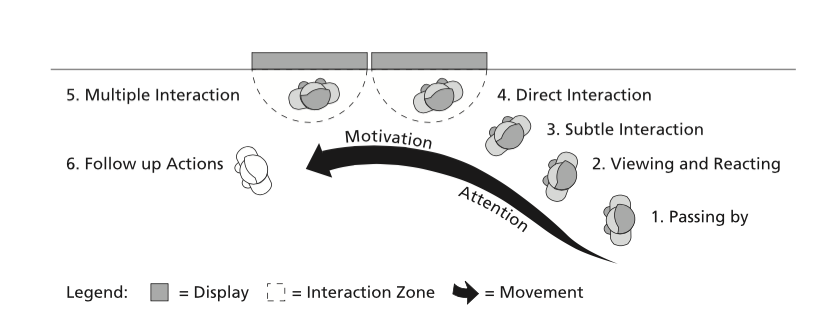
\includegraphics[width=120mm,height=70mm]{Figures/3/TheAudienceFunnel}
\caption{The Audience Funnel}
\label{fig:audience_funnel}
\end{figure}


\subsection{Interaction modalities}
\subsubsection{Body}
\subsubsection{Mobile}

\subsection{Interaction models}

\subsection{Evaluation}

\subsection{Approaches to Research}
\subsection{Methods and tools}







 






% Chapter 3
\newcommand{\hilight}[1]{\colorbox{yellow}{#1}}

\chapter{Attraction attention} % Main chapter title

\label{Chapter3} % For referencing the chapter elsewhere, use \ref{Chapter1} 


\section{Introduction}
This study is a comparative study to investigate how the attention toward the screen could be achieved by evaluating three different techniques shown on the Mensa screen and the old traditional advertisement, This would help to provide idea to design the attention step of the interactive advertisement and get passers-by feedbacks and ideas about these techniques.

\section{Background and related works}
At the early stages of digital advertisement, they were very interesting for people and people would stand for a while and have a look at the content, simply because it was something new with big screens, and now digital advertisements are increasing everyday and has become very common and it is same as Television ads without sound; therefor most people try to avoid seeing them because it is not interesting for them anymore or is not related to them, some how there is a missing link between people and advertisements. The rise of powerful computers and new technologies in the last decades, we have Interactive advertisements that integrate people involvement to make advertising more effective and usable.

Designers of Interactive advertisement have focused a lot on the Usability of the them which obviously should not be avoided but many other factors have not been studied deeply that is why it fails to accomplish their main purpose and are treated like simple posters and ignored. Interactive advertisement should be able to Attract and motivate users and finally allow users to interact in a better way. ``\emph{If they capture attention, many displays seem to fail to motivate passers-by to interact, who have other goals in mind. If, finally, the audience has noticed the dis- play and is motivated to interact, interactive displays seem to fail to deal appropriately with the public nature of interaction, where people may avoid interaction in order to maintain their social role and e.g., not look silly}''\cite{DesignSpace}


Every moment we spend alone, with friends in the crowd, in the concert or party our attention keeps tracks of us and make us aware of the environment and we react differently for different stimuli, so ``\emph{Attention is the process that, at a given moment, enhances some information and inhibits other information. The enhancement enables us to select some information for further processing, and the inhibition enables us to set some information aside.}''\cite{Attention}. Attention is influenced by two different processes (Top-Down \& Bottom-Up). Top-Down process happens when the user has prior awareness (goal) about where to put his/her attention toward and Bottom-Up process happens when the user has no prior awareness and suddenly by an external stimuli move or change attention toward or to something. People walking on pathway or walking in a store or waiting in bus station does not have any knowledge or awareness about an Interactive advertisements located there, nor the researchers tend to speak about it for them, at this situation I believe that the attraction of attention should be a Bottom-Up process for the users to drag them to the screens.

The appearance of objects suddenly or moving objects on the screen or contrasting color can capture attention quicker. Yantis and Jonides (1984) demonstrated that the detection of a target in visual search was markedly enhanced when the target was presented as an abruptly\cite{capturingattention}. And the type of contrast change on an object influence priority in visual search, ``\emph{Both the sudden appearance of an object and sudden changes in existing object features influence priority in visual search.}''\cite{Luminance}

Elaine M. Huang, Anna Koster, and Jan Borchers have researched and discussed on ``\emph{When Does the Public Really Look at Public Displays?}''\cite{WhenPublicDisplays}, in this paper they argued that glancing and attention at large displays is complex and is dependent on many factors like Brevity of glances, Positioning of displays, Content format and dynamics, Catching the eye, Display size, this paper provided some recommendations for each of the mentioned factors.

\section{Approaches}
As discussed earlier the Interactive advertisement would need to first attract the passers-by, Therefor ror the initial attraction attention study, three different types of eye-catching techniques are made to observe which suites best for further research and which side of them should be improved and use them for the interactive advertisement. In this study the of the interactivity or the advertisement itself are not the core study, this study is only to see how many passers-by change their attention and glance toward the screen. 

The definition of glance and ignored toward a screen is briefly given by John Hardy and their colleque \cite{glance} in which they categorized the attention level to three levels as glanced, ignored and watched, glance happens when the passer-by turn his/her head and stares the screen for less than 3 seconds, and ignore is when the person completely does not look or turn his/her head. 

\subsection{Prototypes}
In the following examples the screen background color is set to black and is in full screen mode but with different contents.
 
As you can see in this figure  \ref{fig:Attraction_Attention} these eyes suddenly pop-up when a person passers-by the screen and follows the person by moving its eyeball. The idea behind this is to check if people would react if something abruptly appear on the screen and starts to follow people, This example has very limited movement it is only constraint with limited eye space, but big object with high contrast.

Another example in figure \ref{fig:Attraction_Attention}, shows different colored and sized firework animation, The application will show a random firework for each person on the scene, there are three blocks of fireworks for three persons, the movement of the person changes the location of the firework. In this example there is more object movement and color changes with high contrast.

Jorg Müller \cite{LookingGlass} has investigated that how passers-by notice the interactivity of the public display by showing different representations of body like Mirrored (1) ``\emph{user silhouettes}'', (2) ``\emph{avatar-like}''representations and (3) ``\emph{real user Image}''. In that paper they concluded that mirroring user image is much more effective to attract users and understand the interactivity of the display, but because of privacy policy and because of social attitude like may be someone does not like to be shown on the screen, only Mirrored silhouettes,which is the augmented colored representation of people, will be shown and investigate how much is the attraction toward the screen.  Figure \ref{fig:silhouttee} shows three person's silhouette representation.

\begin{figure}[!htb]
    \centering
    \subfloat[]{{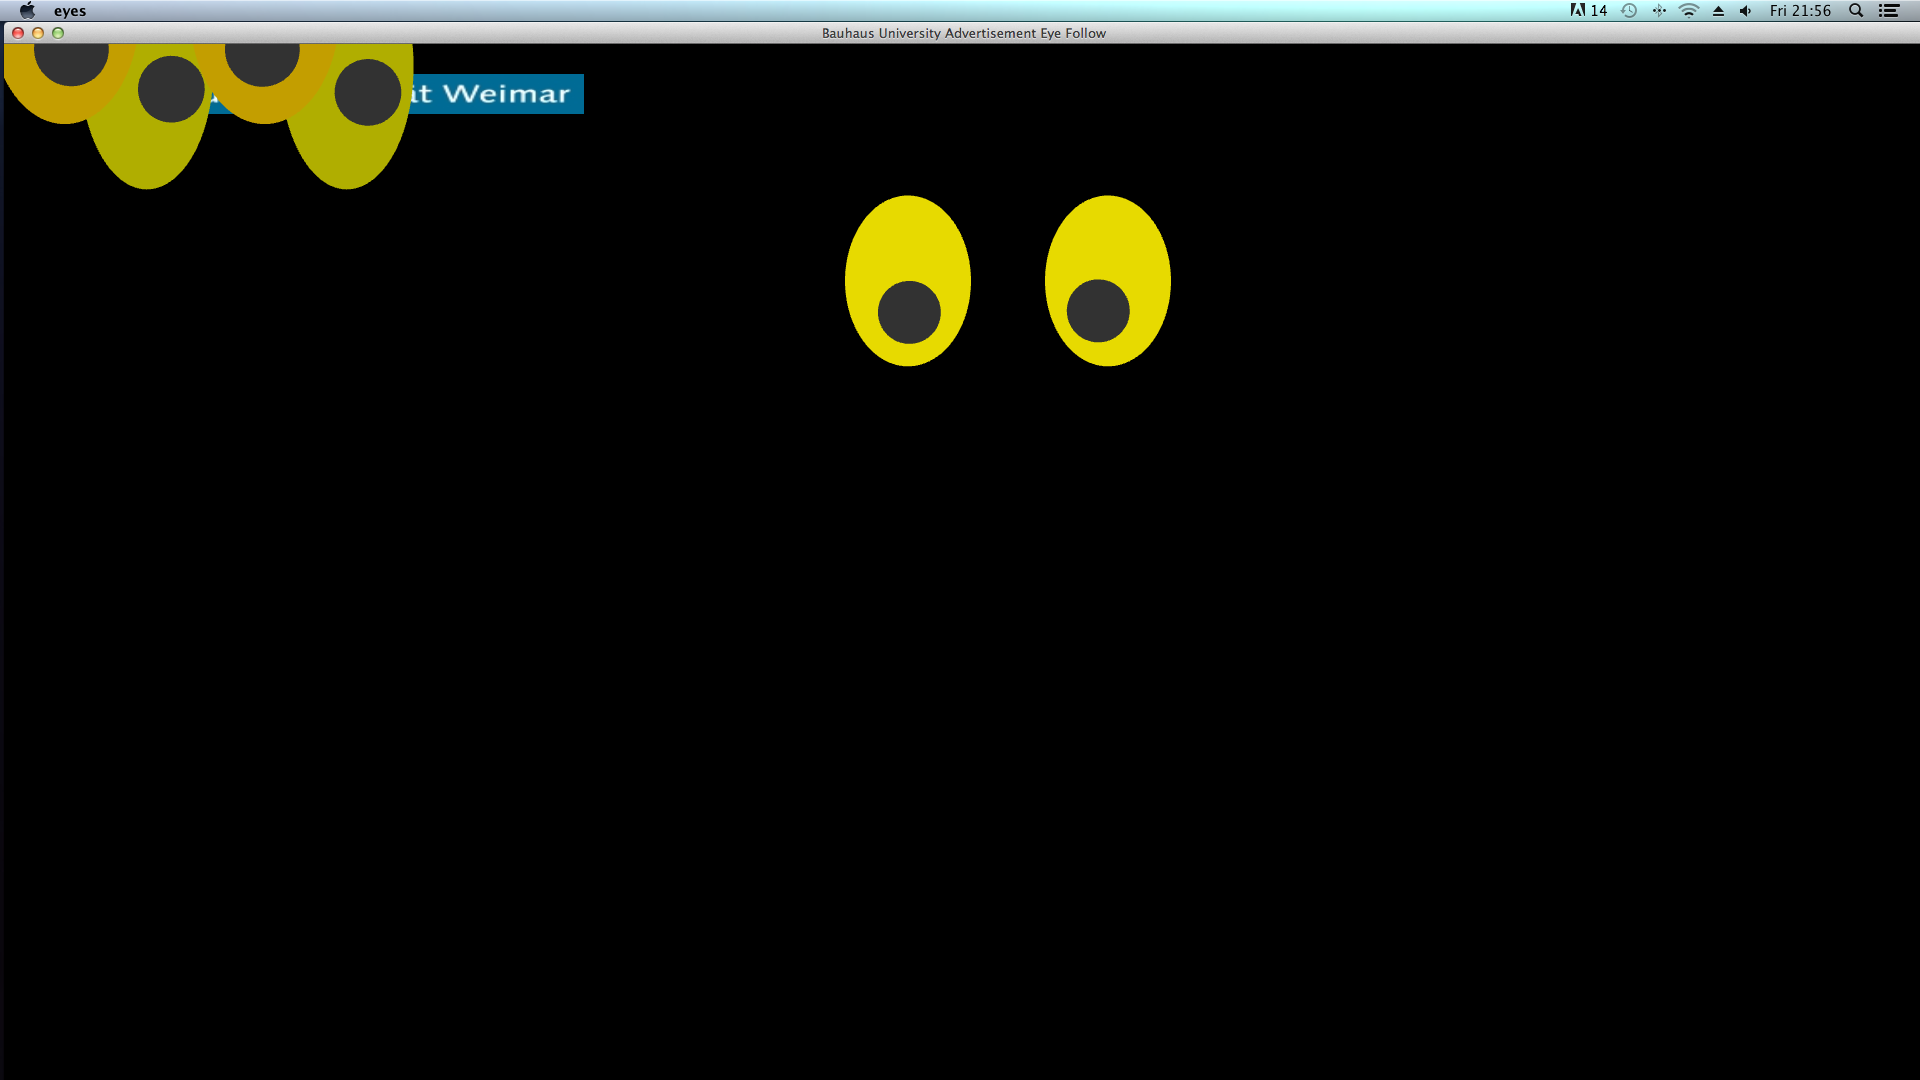
\includegraphics[width=50mm,height=40mm]{Figures/3/eyes} }}%
    \hfill
    \subfloat[]{{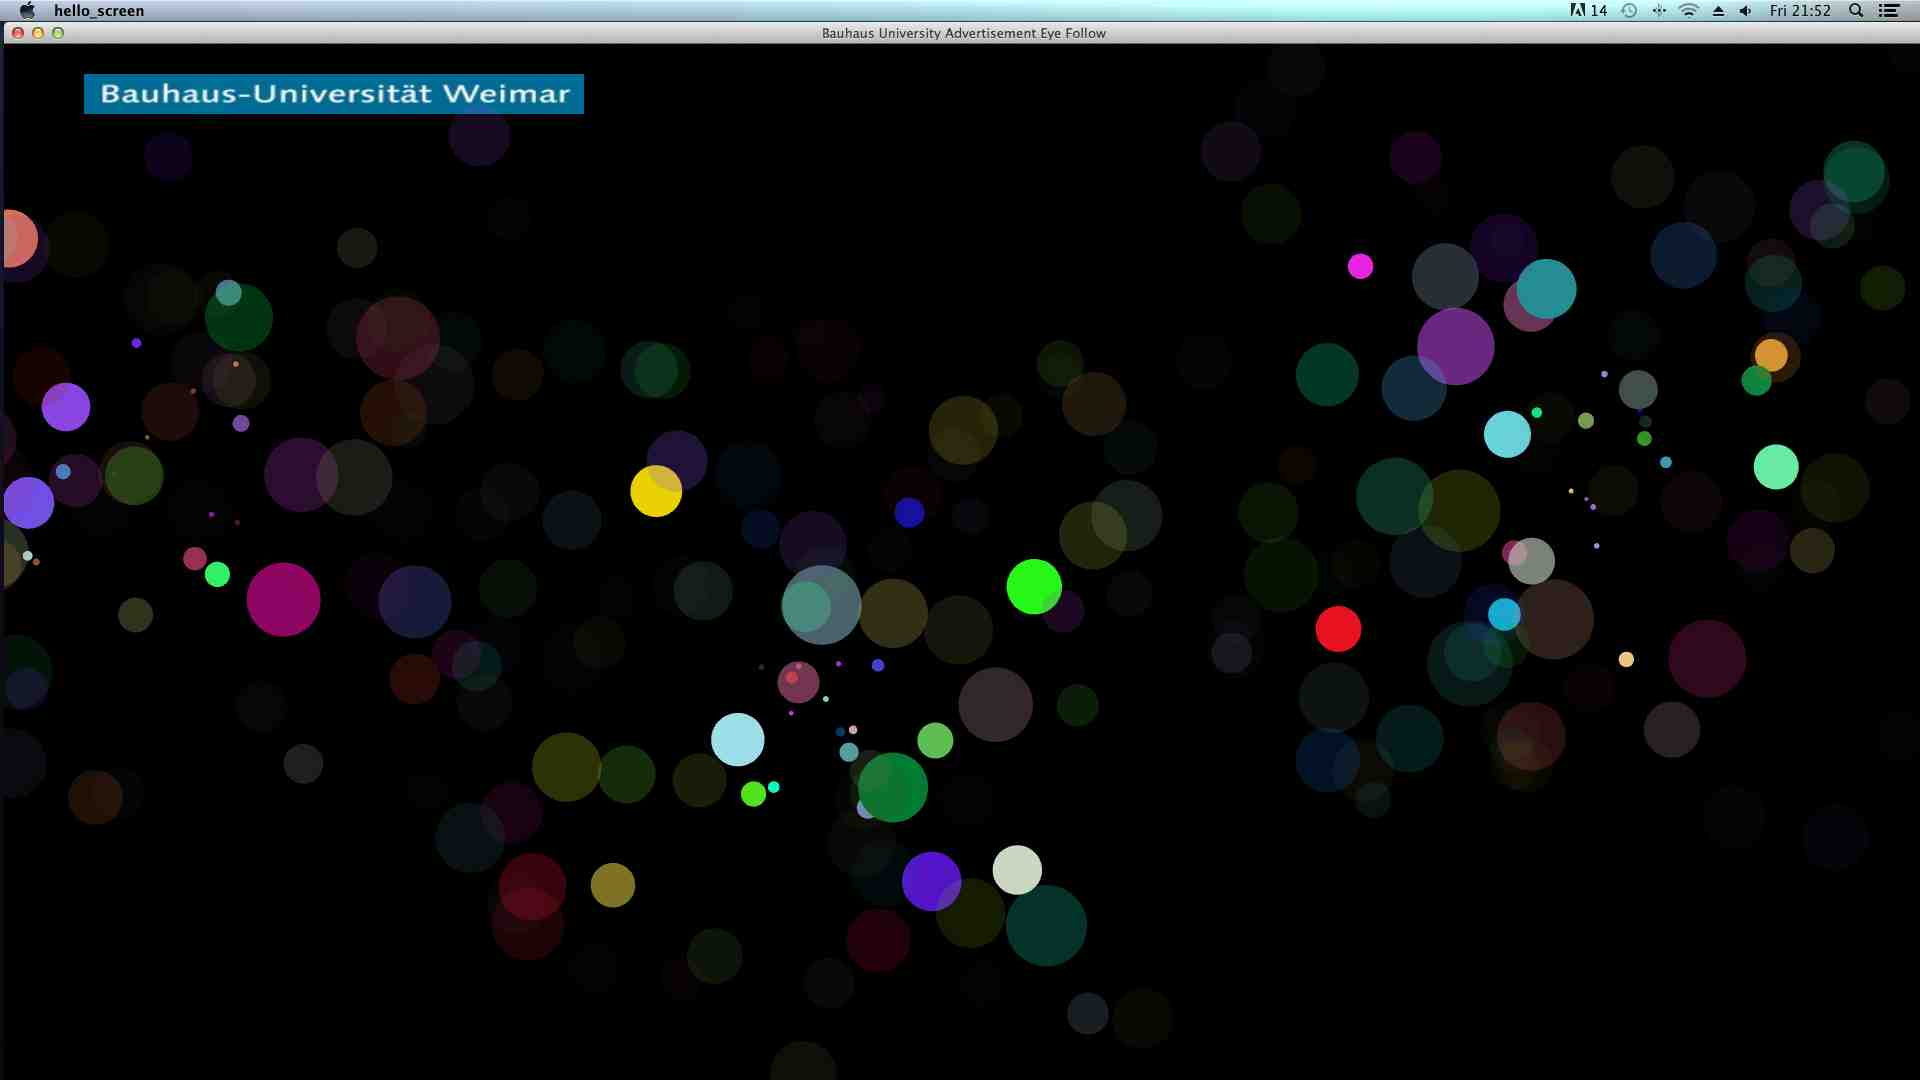
\includegraphics[width=50mm,height=40mm]{Figures/3/fireworks} }}%
    \caption{A: Following eyes  B: Fireworks animation }%
    \label{fig:Attraction_Attention}%
\end{figure}


\begin{figure}[H]
    \centering
    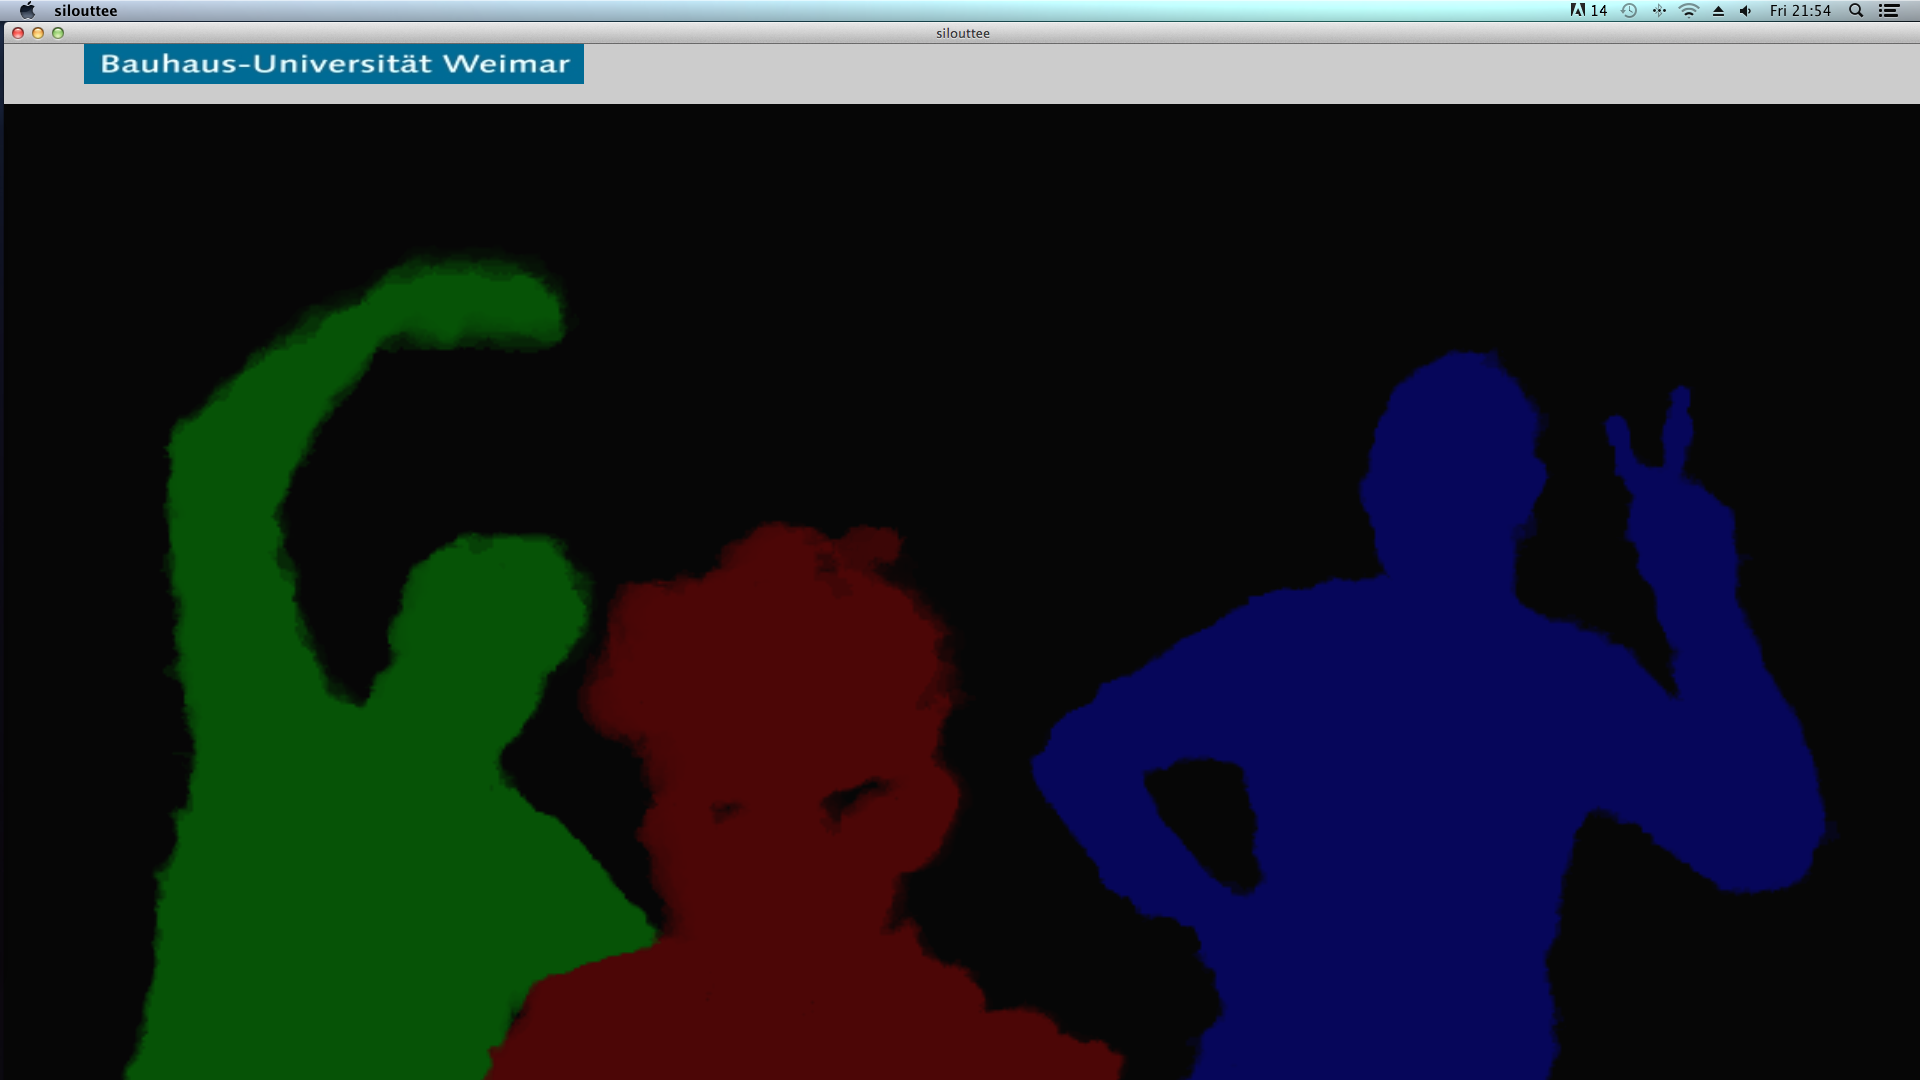
\includegraphics[width=50mm,height=40mm]{Figures/3/silhouttee}
    \caption{Three silhouette representation}%
    \label{fig:silhouttee}%
\end{figure}



\subsection{Hypothesis}

\begin{itemize}
\item \textbf{H1:} Silhouette representation method attracts more passer-bys than other two methods.
    
    \begin{enumerate}
        \item Dependent Variable: Number of people glance per total passers-by.
        \item Independent Variable : Interactive / traditional Advertisement.
    \end{enumerate}
        
\end{itemize}



\section{Study design}

In the beginning the idea was to conduct a some experiment in the lab and investigate about the attention, like doing gaze tracking but it did not suited well for the real life displays, Therefor we came up to a decision to investigate the glance counts made for each individual methods and compare them among each other. 

\subsection{Participants}
Participants were random from university students or employees, basically a broad target that mostely consisted of students and teachers, the participants were taken in consideration that passed in front of the display, The participants who passed from the backside of the screen were not taken in consideration. Non of the participants knew about the methods shown on the screen.

\subsection{Location}
The study was conducted in university Mensa, this location was an ideal location because many students, teachers and university employees go for having lunch and taking coffee breaks and the Mensa gets crowded. The Mensa 14 inch display was used for the study, which was installed near the stairs and already was used for advertisement purpose.

\subsection{Procedures}
The study was conducted for four continues days, and each day only one method was displayed on the screen for two hours at 14:00 oclock, The first day of the study was the passive mode of the screen, where traditional advertisement was displayed and the next three days the attraction attention methods were activated.
One person was responsible for observing and noting the glances made by the passers-by and also noting interesting behaviour of people toward the screen. The other person was responsible to take interviews from the passers-by that glanced at the screen and get more feedbacks of the advertisement in general.

\section{Data gathering}
Three different attraction attention methods and one traditional advertisement of Kasseturm were evaluated each for two hour period from 14:00--16:00 in individual days in Bauhaus University Mensa. Two methods (Observation and Interviews) were used for data gathering during the four day long period.

\subsection{Observation}
Observation was used to count the number of glances the passers-by make at the screen while pass from the front of the screen. A small pilot study was conducted for the observer to find an appropriate location in the Mensa setup to be able to count people and glances without being noticed by passers-by.

The first day, which is a normal advertisement, does not require Kinect Camera, but in order to have same environment for all the days, The camera was installed on top of the monitor to look similar as the other interactive feature.

\begin{figure}[!htb]
    \centering
    \subfloat[]{{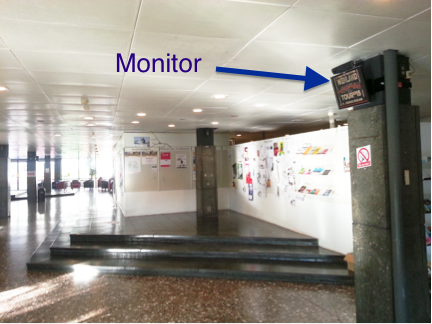
\includegraphics[width=6cm]{Figures/3/Kasseturm_monitor} }}%
    \hfill
    \subfloat[]{{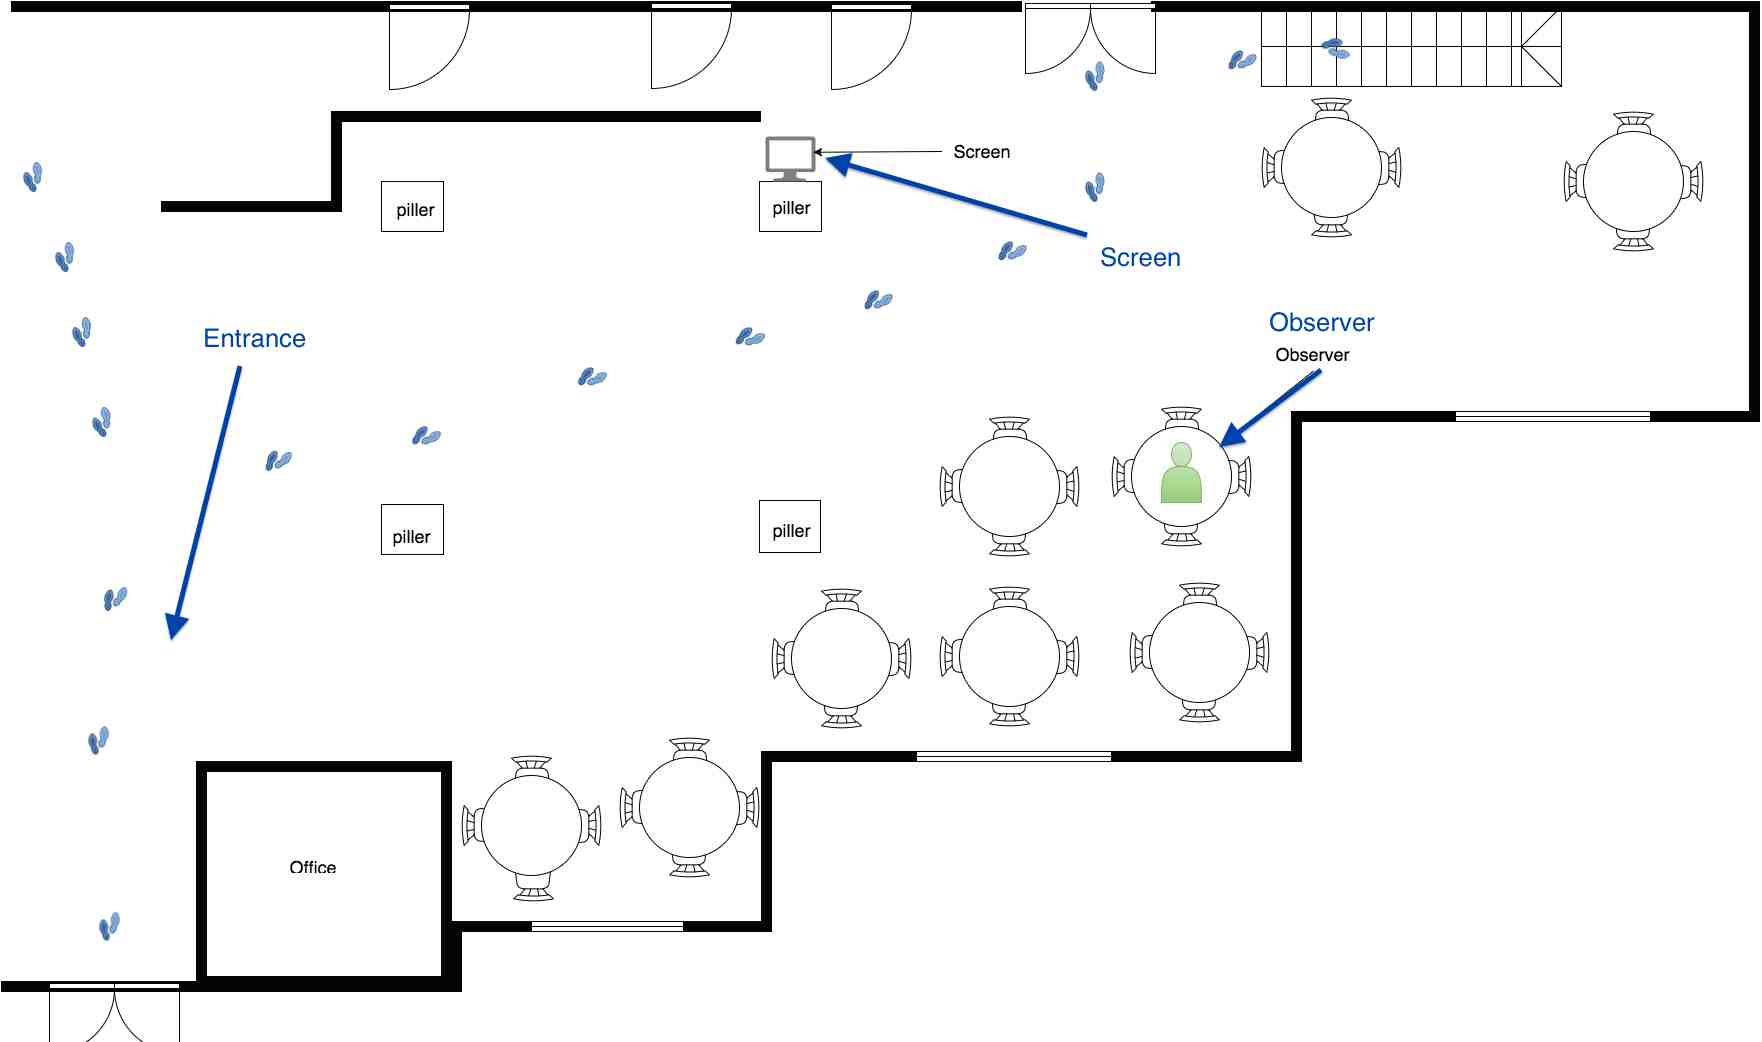
\includegraphics[width=6cm]{Figures/3/mensa_setup} }}%
    \caption{A: Mensa ground floor. B: Kasseturm Advertising monitor. }%
    \label{fig:observation_env}%
\end{figure}

As sheet was provided to the observer to note each 5 min time stamp for two hours, specific letters were defined to detect Male, Female, Unknown gender and at the same time who were in a group and individual and who glanced to the screen. See \ref{AppendixA}.1

%include the info sheet here in appendix

As stated before that observer was given one small pilot study to detect a good location and be able to count and note in the sheet, beside that he was told to write notes if he observes something interesting during the period.

\begin{figure}[!htb]
    \centering
    \subfloat[]{{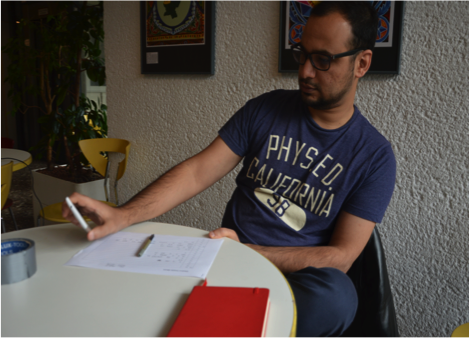
\includegraphics[width=6cm,height=4cm]{Figures/3/hamid} }}%
    \hfill
    \subfloat[]{{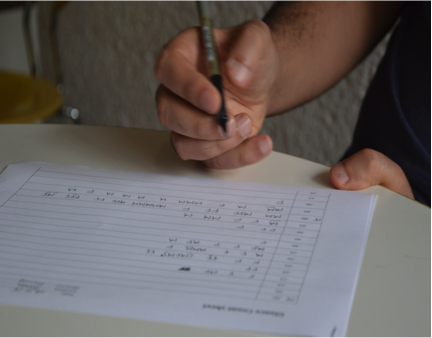
\includegraphics[width=6cm,height=4cm]{Figures/3/observer} }}%
    \caption{A: Hamid Sabri is getting prepared for observation. B: Observer is taking notes on the data sheet.}%
    \label{fig:observation_env}%
\end{figure}



\subsection{Interviews}

During all four day of the observations, 16 interviews were taken from people inside Mensa to get general opinion about advertisement and people preferences what they like and what they avoid about advertisement. Responders were asked to sign the consent form because the interviews were tap recorded for later analyzing.  Each interview took around 6 minute in average. All interviews were transcribed separately for further data analyzing.
See \ref{AppendixA}.2 for consent form and  \ref{AppendixA}.3 for the questionnaire.

\section{Findings}
To have accurate findings, they are categorized as bellow.

\subsection{Observation findings}

Observational data for glance count and people passed by the screen were gathered and results to the bellow findings.

% table
\begin{table}[!htb]
\caption{Results of attraction attention methods}
\label{tab:treatments}
\centering
\begin{tabular}{l l l l }
\toprule
\tabhead{Method} & \tabhead{Glanced \%} & \tabhead{ingnored \%} & \tabhead{Total } \\
\midrule
Traditional & 9 \%7.6 & 109 \%92.3 & 118\\
Silhouette & 21 \%15.2 & 117 84.7 \%92.3 & 138\\
Following eye & 10 \%12.98 & 67 \%87 & 77\\
Firework & 6 \%10.1 & 53 \%89 & 59\\
\bottomrule\\
\end{tabular}
\end{table}

As can be seen a lot of from the table above Silhouette attention attraction technique received the highest number of glances 21 out of 138 compared to other techniques, Following eye technique was the second most attracted technique probably because of its contrasting color and funny.

\hilight{Attraction level has not changed between male and female}

So the decision would be to use silhouette technique for further advertisement application. 


\subsection{Interview Findings}

Interview transcripts were individually coded to generalize the responder?s opinions on the advertisements. I created two main sections from the interviews that what makes a Good Advertisement, and what makes a Bad Advertisement and related all responses to these sections a lot of codes were analyzed and grouped together to make sub sections and sub-sub-sections.

\subsubsection{Good Advertisement}
A lot of categories have been found after coding the interviews the chart in Appendix A, show all the categories and sub categories with the correspondent code from the interviews and even some codes were directly also placed as a category instance. The bellow list describes some of the important categories retrieved from the diagram.


\begin{enumerate}
\item \textbf{Content} \\
Interactive advertisements attract more people than traditional advertisement.
Responders like to have more Funny contents than any other restrict informational advertisement; ?just make it funny like make a joke or something but something in a very good one that is really difficult?, ?it should be very not very serious?, ?Yeah mostly I like funny things that the main concept is shown in different way like in funny things?, ?I like advertisement that are somehow have humor?. 	 \\

At the same time responders would like to see some useful, true, sensible facts and main idea of advertisement; ?an offer if it is clearly mentions that okay that you save this much or you get this or that, that is like a clear message?,  ?you have to focus on the main things that will happen in the event which will attract people will come.? \\

Furthermore contents of advertisement should be small and understandable; ?the advertisement should be clear too. ?, ?when you have too many numbers and too much to read then it is confusing?  ?Add some pictures based on the advertisement what do you want to show. ?, ?Not many text in advertisement?,? Have a good design, not too crowded with information?, ?Well defined subject, and shorter contents, because we don?t like reading long things usually no  body likes to read?.  \\

Another important thing was Context Based contents, the users liked to see things related to their surroundings; ?if I am standing near a shopping center it should tell me that what kind of shops are there and what I could buy from there.?  ?It should show movies of the actor I like?. \\
		
		
\item \textbf{Creativity} \\	
People like to see very new and creative things happening in advertisement; ?something that catches your attention in a way that you haven?t seen before?, ?like seeing something out of ordinary?. Introducing new ideas, artistic; ?as I am musician you know kind of creative person I like if it something special inside not it is just like for example if it is advertisement of milk ?, ?Which can be something un-expectable probably also ?, ?in general I would say yes as long it gets creative?


\item \textbf{Style} \\	
The style of advertisement plays key role in terms of color and size as stated by responders; ?may be should be more should be more colorful?, ?my eyes are attracted to so hard things unless there is something big enough things ?, ?Use the bright color. ?, ?You have to be clever in using colors okay because color mismatch does not attract the eyes?, ?when it is really just like an art like you have a picture you some impression or illusion?.

\item \textbf{Location} \\	
Responders like to see advertisement while they are on the way, they don?t get annoyed if advertisements comes on their way and some probably take a look to them too, but heavily they do not like advertisement while they are at home or watching program in TV or Internet, ?I think the street is better?

\item \textbf{Interactivity} \\	
Some liked to have some sort of interactivity to experience like playing games; ?it is good like if you have a game, it would better to have a preview of the game on the screen or just like something like even people could interact with it like get an experience of the game?, ?if the screen will also be interactive so you can interact with the with the something you are advertising.?

\item \textbf{Mean} \\
Different means were mentioned like larger screen, sound, banners for good influential advertisement.

\item \textbf{Motivation} \\
One of the responder pointed that the advertisement should motivate users in a natural way and should be from unbiased point of view; ?I prefer to buy in a natural way. The company should know who are using their product the power users who that have a lot of influence you know if you have good connections with the guitarists who have like actually like you know people listen to his opinion I think you have to reach out to the guitarist but once you know the guitarist is gaining something from that guitar maker then I don?t trust that company, It should be like completely unbiased, I think that is the kind of advertisement I listen to. ?. \\

Others suggest that advertisement must motivate for healthy diet and sport; ?if it reminds me to do stuff like do more sport or eat healthier or anything that has a good purpose?

\item \textbf{Other categories} \\
Many other categories were also extracted for a good advertisement like Goal of advertisement, Audience, Purpose and motivation, for more detail look at appendix A.
		
\end{enumerate}



\subsubsection{Bad Advertisement}
The bellow categories were derived from the interviews that make an advertisement feel or look bad, and we should not avoid using in advertisements.

\begin{enumerate}
\item \textbf{Style} \\
There exist different styles that advertisement makers follow but texts or photos are blinking; ?try not to use anything would be blinking okay because that is really annoying okay because even so if you are not looking at it is still effecting?. Using of mismatched colors in advertisement is certainly a bad idea; ?color mismatch does not attract the eyes?.

\item \textbf{Annoyance} \\
Most of the responders felt annoyed by almost all advertisements because they contain some sort of similar features like repetitions; ?it should not be like repeating itself over and over and over again?, ?I like advertisement apart from watching it again and again?, ?Hmm if I see the same advertisement again and again that is annoying. \\
? Other feature is destruction, which does not allow a person on focusing on something; ?Not just like something popping up in front of your face?, ?for example in middle of the serial or a movie that i am watching and an advertisement that is I don't like because it makes me destructed now I just can't focus on things for view minutes you have to leave what ever you were?

\item \textbf{Motivation} \\
Advertisement in general motivate people in their own way to attract customers, which people make not like it, for example sudden appearance of something in the screen or what users do not like to see but they are forced to see; ?usually you are forced to see them because you are watching something or doing something and suddenly it comes and it disturbs you?, ?it is trying to convince me of something only for to consume or buy and then I mean I don?t? want?

\item \textbf{Content} \\
Some advertisements exaggerate on their products or even say lie; ?it is like magnificent thing and nice pen okay and then it is just a pen, okay?, ?They are all lies?. Showing inappropriate content are heavily disliked; ?whenever I go and access the Internet okay? A lot of advertisement comes to my face and most of them are inappropriate. \\
Stuffs like that I don't like them at all?, ?for example some perfume ad which would the a woman in a very degrading position or for example mocking someone believe or something just to catch the attention that is probably to offend people that is what would annoy me a lot. ?. The use of ugly and old people is also not welcomed.

\item \textbf{Duration} \\
Long lasting advertisement are always boring and waste of time, most of the responders said that they would prefer short advertisements.

\item \textbf{Other categories} \\
Many other categories are also extracted from the interviews like location, Confusing advertisement, Controversial ads, amount of ads and types of ads that were not liked by responders. For more information see Appendix B

\end{enumerate}


\section{Discussions}

\section{Conclusion} 



% Chapter 4
\chapter{Advertisement decision} % Main chapter title

\label{Chapter4} % For referencing the chapter elsewhere, use \ref{Chapter1} 
\newpage



\section{Introduction}
At the time of industrialization, industries compete on product quality, and modern organizations focused more on delivering services. But now services and products are hardly able to be distinguished because they provide various offers and consumers lose themselves in them. Peter van Waart describes in his paper that ``\emph{In the last two decades however, economical developments resulted in the experience economy: a new era of marketing and branding, in which traditional advertising is becoming less effective and meaningful experience branding is key}'' \cite{Meaningful_ad}.  Therefor economical developments have changed from time to time and are now emerging from economical experience in which factors like price-reduction is not so important. But experience factor has become the central part for the development. Any advertisement that explains a product features might fail to achieve people satisfaction because people’s experience might not have considered in it. As Joško Brakus \cite{Brand_experience} explains the measurement of brand experience and how it can effect on product loyalty.


\iffalse
At this era the technology is highly advanced and most people especially youngsters are much familiar like using smartphones, tablets. At the same time there are many other developments in sensing technologies like body tracking, hand recognition. By using these technologies different interactions are possible and very attractive and funny interactive advertisement can be developed so that it could attract and engage more participants.
\fi

To create a true meaningful advertisement and gain people satisfaction, the advertisement should be created so that people and stakeholders be satisfied.
The development of advertisement requires many steps and the initial step is to create content.It happens normally by creating a \emph{Focus group} of stakeholders to be able to fully discuss the advertisement requirements. \emph{Focus group} is a small group between six up to ten participants that joint together in comfortable and quite place to discuss on a specific topic domain. As described by Jenny Cameron ``\emph{Focus groups can be exhilarating and exciting, with people responding to the ideas and viewpoints expressed by others, and introducing you, the researcher, and other group members to new ways of thinking about an issue or topic }''\cite{FocusGroup}. One of the example of a \emph{Focus Group} is discussed in Florian Alt \cite{mobile_focus_group} that talks about the process of how the focus group was conducted for a mobile contextual display systems.

As a computer scientist, there had been no chance to create an advertisement, and this was the first opportunity to make one. After negotiating with University communication department and then discussing with University marketing department, finally the decision was made to make an advertisement for \emph{Bauhaus-Walk}\footnote{Bauhaus Walk: https://www.uni-weimar.de/en/university/profile/bauhausatelier/bauhaus-walk/, last accessed 26 may 2016}. What I knew about \emph{Bauhaus-Walk} was that it conducts tours about Bauhaus for tourists in Weimar. But in-depth goal and motivation of this program was not clear for me. I did not know what kind of advertisement they wanted, what message they wanted to convey through the advertisement.
   
Therefor, there was a need to conduct a \emph{Focus Group} to do requirement analysis on \emph{Bauhaus-Walk} program. This was mainly meant to understand many aspects of Bauhaus-Walk and collect the required parameters for designing the advertisement (interactive and non-interactive). Because of time limitation and participant schedules two sessions were arranged in two different dates to cover all topics and discussions. This chapter describes the main theme and goal for \emph{Focus Group} and reports all the processes that were taken. Like, how participants were invited and what was being discussed and more focused on each session. How data was gathered and what techniques were used to analyze them. The document presents all the findings and outcomes in details and related discussions and conclusions.

\section{Research Questions}
To design and create the \emph{Bauhaus-Walk} advertisements, it was required to collect the below information from the Bauhaus-Walk members. With the help of those information a very relevant and meaningful advertisement could be developed that could speak by itself for \emph{Bauhaus-Walk} and at the same time it should be entertaining and funny and fit for both interactive and non-interactive advertisement. Therefor I needed to understand the bellow aspects of \emph{Bauhaus-Walk}.

\begin{enumerate}
\item Who is (are) the target group?
\item What are the existing Bauhaus-Walk advertisement medium?
\item What are the peak times in the year and famous locations for Bauhaus-walk tour?
\item What are important aspects of Bauhaus-Walk from their point of view?
\item What could be a suitable advertisement theme and content?
\item What interactions should be integrated in interactive (body \& Mobile) advertisement?
\end{enumerate}



\section{Study design}
Focus group was designed in two sessions because all the participants could not be present at the same time or date. And by doing this, there was enough time to analyze the first session and discuss the findings in the second session with new participants and get their point of views. The first session was more related to gathering general information about \emph{Bauhaus-Walk} program and second session was more in depth discussions on the advertisement decisions and prototypes.

\subsection{Participants and Environment}
The Focus Group in the first session consisted of three participants, and in the second session it consisted of two participants. The participants of both focus groups were tour guides of \emph{Bauhaus-Walk}, they had been providing tours for more than a year and knew the aim and vision of \emph{Bauhaus-Walk}. Participants were invited through Doodle\footnote{Doodle: http://doodle.com/de/, last accessed: 26 May 2016}, where varieties of date slots were available to select, in which a short introduction of the aim of the Focus Group was also described. Both sessions lasted for 90 minutes.


\begin{figure}[H]
    \centering
    \begin{subfigure}[H]{0.45\textwidth}
        \centering
        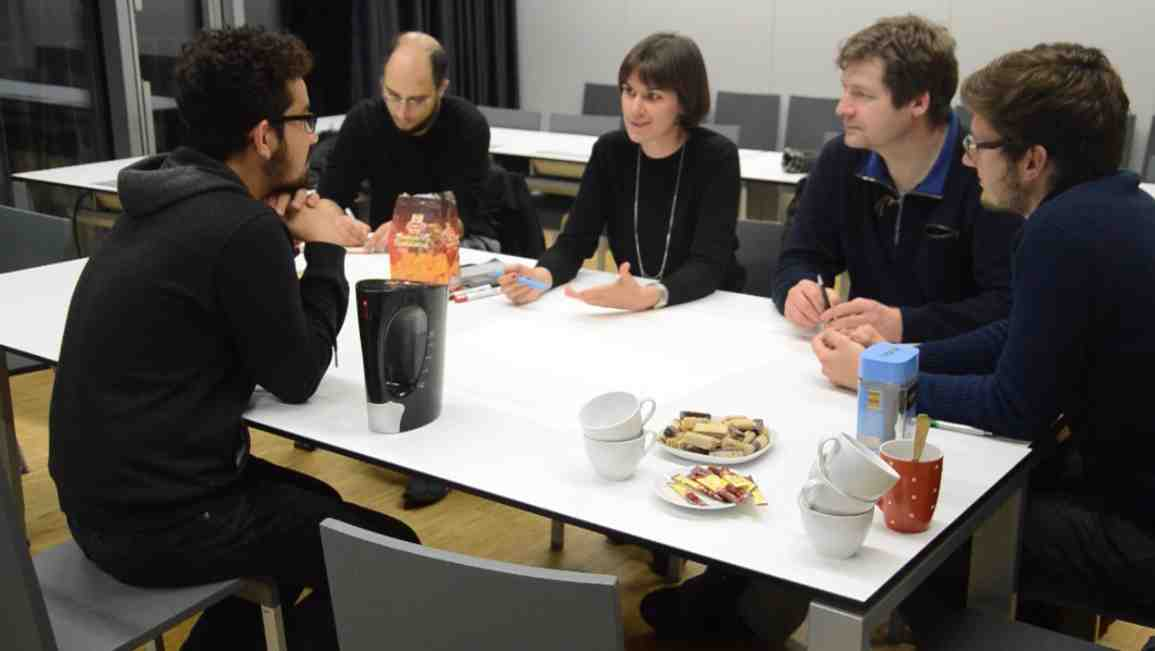
\includegraphics[width=\textwidth,height=4cm]{Figures/4/focus_group_s1}
        \caption{1st Session focus group }
        \label{fig:focus_group_s1}
    \end{subfigure}
    \begin{subfigure}[H]{0.45\textwidth}
        \centering
        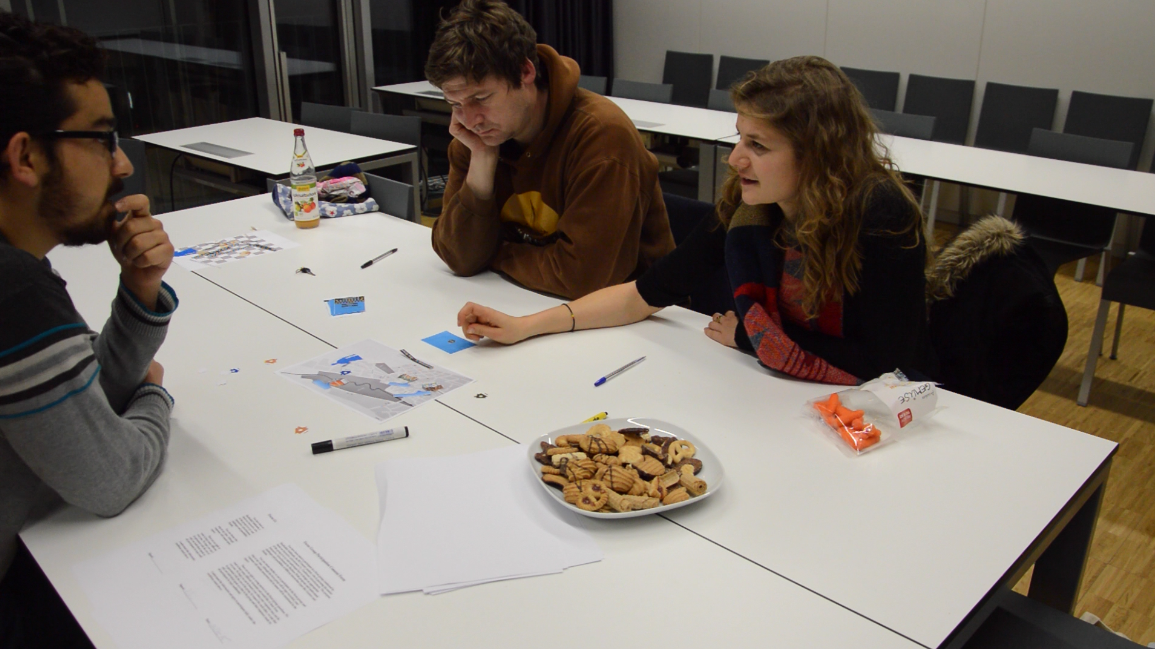
\includegraphics[width=\textwidth,height=4cm]{Figures/4/focus_group_s2}
        \caption{2nd Session focus group}
        \label{fig:focus_group_s2}
    \end{subfigure}
    \caption{Focus group sessions}
    \label{fig:Focus_group_sessions}
\end{figure}

The Focus Group was held inside the \emph{DBL}\footnote{DBL: Digital Bauhaus Lab} building meeting room, where we had enough space to make a group circle. Participants were offered coffee and biscuits at the beginning or end of the session to feel comfortable and relaxed for discussion.


\subsection{First session}
This session was an exploratory session over \emph{Bauhaus-Walk} program. And it was a good start for me to investigate thoroughly on that domain to create the advertisement prototypes for the next sessions.


\subsubsection{Procedures}
Participants were warmly welcomed and asked to feel comfortable by having biscuits and coffee. I introduced myself and asked them to introduce themselves. This helped to understand each others professional background and interests.


\begin{enumerate}
\item Introduction \\
Brief introduction on advertisement and interactive advertisements were given to participants to understand the possibilities of existing technologies and the use of them in advertisement field. Some interactive advertisements were introduced with their relative interaction techniques. The agenda and goal of Focus Group was also described to have a wide picture of what is going to be done till the end of this semester.

\item Consent Form \\
Each participant was asked to sign the consent form before actual discussions to make sure that they agree to participate and be video recorded.

\item Discussion session \\
After introduction, the discussion started on below questions. Because there was limited number of participants I could not divide them in to groups to discuss in detail and do comparative study among the groups. But they were given an empty big paper sheets to draw and write what come in their mind during discussion. This kept track of their thoughts and became easy to generalize their opinions. During the discussion Patrick Tobias Fischer was asked to write notes on the discussions.

\begin{enumerate}
\item   What kinds of advertisements for Bauhaus-Walk are there?
\item   Who join the Bauhaus-Walk program in general?
\item   What could be a suitable theme of Bauhaus-Walk for the Interactive advertisement?
\item   What would be the content of the advertisement?
\item   How to motivate passer-by to be engaged with the advertisement?
\item   How to engage passers-by with the advertisement?
\item   What kind of Gesture and Mobile Interactions should be used?
\item   How to motivate passer-by to join the actual Bauhaus-Walk tour?
\item   Is there anything else we need to discuss on Bauhaus-Walk Advertisement? Any new angle?

\end{enumerate}


\end{enumerate}


I was responsible to carry on the entire discussion and Patrick Tobias Fischer was doing the note taking during the discussion. He noted important information extracted from our discussions so that I could later look at them beside that, the entire discussion was also video recorded for analyzing.



\begin{figure}[H]
    \centering
    \begin{subfigure}[H]{0.45\textwidth}
        \centering
        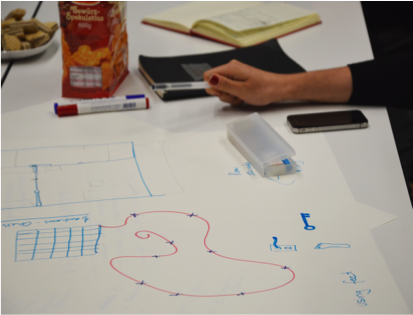
\includegraphics[width=\textwidth,height=5cm]{Figures/4/drawings}
        \caption{Drawing sketches}
        \label{fig:focus_group}
    \end{subfigure}
    \begin{subfigure}[H]{0.45\textwidth}
        \centering
        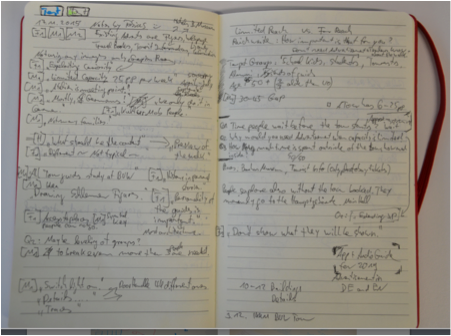
\includegraphics[width=\textwidth,height=5cm]{Figures/4/notes}
        \caption{Observation notes}
        \label{fig:meeting_room}
    \end{subfigure}
    \caption{Discussion Session}
    \label{fig:observation_env_observation_note}
\end{figure}


\subsection{Second Session}
Based on the first focus group's discussions and the participant's nice ideas, which are mentioned in finding section, two different paper prototypes of advertisement were made to dig more in detail. The participants were given the prototypes to play with them and explore their own way of designing the advertisement and interaction.

The basic ideas were designed to help the participants to think more and come up with some more ideas and at the same time should be in the context of Bauhaus-Walk program.

\subsubsection{Procedures}
\begin{enumerate}
\item   Short introduction was given on Interactive Advertisement thesis.
\item   Consent forms were handed to sign for video recording.
\item	Short motivational video of interactive advertisement was shown.
\item	Two paper prototypes that are mentioned above (Bauhaus chess and Map) were introduced.
\item	Possible interactions were shown to them.
\item	Participants were asked to comment on prototypes and come up with new ideas and interactions.
\item	They were asked to design their own prototype.
\item	Integrate some fun ideas with prototypes.
\item	What contents should be included in the prototypes.
\item	How to gather and collect those contents.
\end{enumerate}

\subsubsection{Prototypes and discussion}
Two functionalities prototypes were explained to the participants and how the prototype originated from the previous discussions. A short description to these prototype are give below. 
\begin{itemize}
\item \emph{Bauhaus-Chess Prototype } \\
This prototype was chosen because of the historical background of this amazing chess game that was developed by Josef Hartwig\footnote{Josef Hartwig: http://bauhaus-online.de/en/atlas/personen/josef-hartwig, last accessed: 26 May 2016}. The shape of the chess piece defines the movement direction of itself on the chessboard. The goal was to show the chess on the advertisement screen and show one piece at a moment and let users to move the chess in the right direction by some sort of gesture.


\begin{figure}[H]
\centering
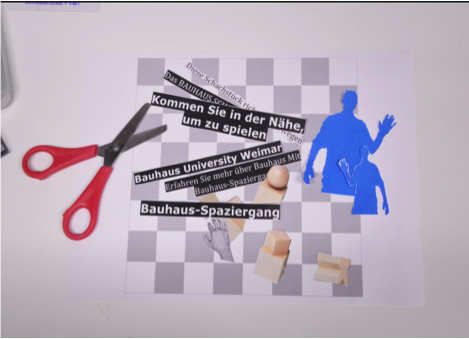
\includegraphics[width=0.8\textwidth,height=7cm]{Figures/4/chess}
\caption{Chess prototype }
\label{fig:chesspro}
\end{figure}


\item \emph{Map Prototype} \\
This prototype was to show a city map of Weimar on the screen with possible interactive famous places of Bauhaus. The interaction idea was to map physical /mobile cursor movement of a person on the map. This interaction let user to explore the target places by reaching to those locations. Maximum five places were to be explored by one person to finish the interaction.


\begin{figure}[H]
    \centering
    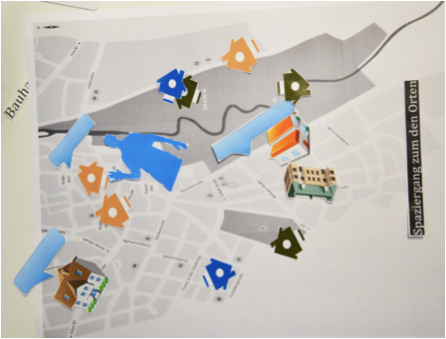
\includegraphics[width=0.8\textwidth,height=7cm]{Figures/4/map}
    \caption{Map prototype}
    \label{fig:mapprot}
\end{figure}


\end{itemize}


After prototype got explained to the participants, they were asked to bring their own ideas and ask questions. This phase was to find possible issues and how to enhance one of them to be used for the final advertisement. The consideration was also that any prototype selected should be valid for non-interactive, body interactive and mobile interactive advertisement all at the same time.

\begin{figure}[H]
    \centering
    \begin{subfigure}[H]{0.45\textwidth}
        \centering
        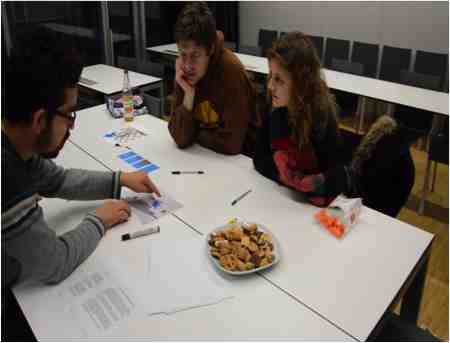
\includegraphics[width=\textwidth,height=5cm]{Figures/4/show_map}
        \caption{}
        \label{fig:showmap}
    \end{subfigure}
    \begin{subfigure}[H]{0.45\textwidth}
        \centering
        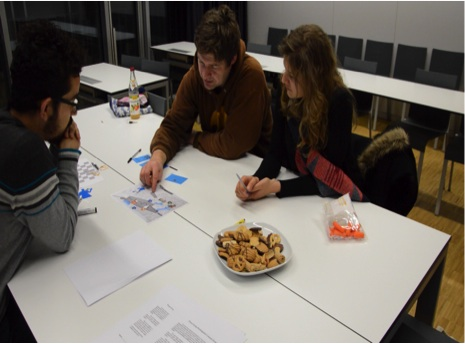
\includegraphics[width=\textwidth,height=5cm]{Figures/4/tell_map}
        \caption{}
        \label{fig:tell_map}
    \end{subfigure}
    \caption{Explaining and discussions on prototypes }
    \label{fig:explaining_and_discussion}
\end{figure}

\subsection{Data Gathering}
The data gathering of the Focus Groups were done in a way that could be very easy to be analyzed and generalized in very little amount of time. 


\begin {itemize}
\item   The participants were encouraged to discuss the issues on a piece of chart using drawings and texts this helped the participants to focus on their ideas and build the ideas in a more better way and at the same time that helped the research to have a summary of their opinions and thoughts 
\item   They could make summary of their discussion on the paper so that they and I fully understand the topics. see Appendix (\ref{app:Sk1}, \ref{app:Sk2} and \ref{app:Sk3}) for sketches.
\item   Tobias Patrick was taking notes to cover up everything we discussed.
\item   All the sessions were video recorded for full detailed analyzing. 
\item Photos were also taken from the participant while discussing ideas, and also from the sketches they drew.
\end{itemize}


All of the above resources were analyzed by going through each of the sketches and each notes that were written. And all the videos were seen many times to check if some ideas were not clear in the sketches or notes. 


\section{Findings}

\subsection {First Session Findings}
The below sections are extracted from the long discussions, and analyzing video and drawn charts.


\subsubsection{Bauhaus-Walk}
\emph{Bauhaus-Walk} is a project that is run by university students to show more about Weimar and Bauhaus culture to the world. They give small tours to group of maximum 30 people. The tour shows studying conditions student, living style of people and giving excursion to historical places.

Tour guides are from different backgrounds like architecture, urbanism and design and each of them shows various aspect of Bauhaus by their own stories. And interrelate the stories with the facts and then connect them to the places in Weimar. The most important for the tour guides are not just the buildings, but also the small details inside the building that most people do not focus. The tour guides want to be the voice of those unspoken stories for the tourists.


\subsubsection{Current Advertisements}
Current existing advertisements for Bauhaus Walk is through different mean as listed below.

\begin {enumerate}

\item	Web: \\
\emph{Bauhaus Walk} is advertised in the Bauhaus University Weimar webpage\footnote{Bauhaus Walk: \url{ https://www.uni-weimar.de/en/university/profile/bauhausatelier/bauhaus-walk/}} and in Weimar tourist information page\footnote{Weimar tourist information: \url{http://www.weimar.de/homepage/}, Last accessed, 4th Jan 2016}.

\item   Print: \\
\emph{Bauhaus Walk} programs are advertised in flyers and leaflets at different locations. The flyers could be found in tourist information center, \emph{Bauhaus Museum}, calendar of Weimar and in travel leaflets. 

\item   Books: \\
Bauhaus Encyclopedia has mentioned \emph{Bauhaus Walk} too. 

\item   Oral: \\
Mostly the people, who have already taken the program once, publicize \emph{Bauhaus Walk} to their friends, relatives.
\end{enumerate}

\subsubsection{Tour participants}
Most of the people who join the tour are from elder people aged between 45-65 years old and others are adults and children. Adults largely learn about the program trough web and the elders learn from the tourist information centers and books.  Often the participants are German and do not understand English language.


\begin{figure}[H]
    \centering
    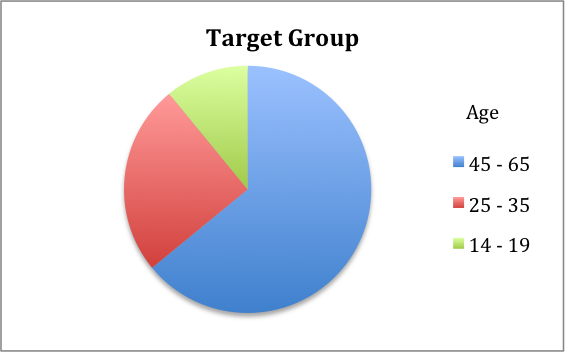
\includegraphics[width=8cm, height=5cm]{Figures/4/target_group}%
    \caption{Tour participant average ages}%
    \label{fig:target_group}%
\end{figure}


\subsubsection{Peak Tour times}
In Average 5000 people take the tour each year. April, May, September and October are the peak months that people take the tour because of the good weather condition. The amount of people per tour is about 25 people, but in winter the amount declines to five to six in one tour.

\subsubsection{Possible advertisement location}

\begin {enumerate}

\item	Tourist Information. \\
This is a good place to put Bauhaus-Walk advertisement because 
\begin {itemize}
\item	Random visitors from different places and cities come here and want to know about Weimar in general. 
\item	Heavy traffic of people.
\item	This is the only place to get Bauhaus-Walk tickets in advance.
\end{itemize}


\item	Bauhaus Museum. \\
This could be another good place, but people have to pay to enter to this museum, so there will be limited people but who
\begin {itemize}
\item	Are very interested in Bauhaus.
\item	Likely to go on tours.
\end{itemize}


\item	University main building. \\
Main university building is a more open place for all visitors; there are many factors as stated below.

\begin {itemize}
\item	People from different background.	
\item	People from different age, more youngsters like students.
\item	Interested people in Bauhaus.
\item	It is close to starting point of Bauhaus-Walk tour.
\end{itemize}


\end{enumerate}


\subsubsection{Content of advertisement}
Participants pinpointed on very important things about the content of advertisement, with which the advertisement got clearer and clearer. As a result \emph{Bauhaus-Walk} could be categorized in to many different aspects of as mentioned below.


\begin {enumerate}

\item   Objects \\
There are objects that are introduced during the tour for the tourists. A good idea would be to show those objects on various locations on the map that belong to.
\item   Stories \\
\emph{Bauhaus Walk} tour guides have many stories to tell about the walk and about their own backgrounds. One of them said ``\emph{Probably our walk is to sum it up, consists of stories we are actually telling stories, not just talking about history, not just about facts but our own personal stories and stories that were told by former students, so we are kind of raping the history in to personal stories, and we want to say that hay, we are students from different faculties and we want to tell the stories by different ways, and that is not a bad thing, because based on historical fact that there has not been the same Bauhaus in Weimar, there has been so many different teachers and students and they all had a different idea that what Bauhaus could be and I think we still kind of incorporate that the fact that no Bauhaus tour would be the exactly the same like the others before.}''
\item   Histories, Facts, Places \\
The content of advertisement could also be related to history of Bauhaus. How it is known to world, what were and are the innovations.


\end{enumerate}

\subsubsection{Interaction of advertisement}
Based on the examples that were shown at the introduction, participants liked hand gesture and some other techniques and gave the below possible technique ideas.

\begin {enumerate}
\item   Hand gesture Interaction. \\
The below two kinds of interactions were discussed each containing different contents. 

\begin {itemize}
\item   Hovering: \\
By showing the Bauhaus map on the screen with the most important elements, the users should be able to look at the items by moving their hands on top of it. The items could change its status when hovering for example if there is a light object shown it should turn on or something like that.
There could be famous places shown on the map that \emph{Bauhaus-Walk} tour focuses the most. And by hovering the hand on some more information like a picture or a related info to that places should be shown.

\item   Performing a specific gesture:\\
There are many objects that have specific characteristics and those details are described in the tour. So the idea was to bring those objects in action and allow users to perform those actions. For example, show a 3D environment and the user should be able to perform a gesture, like opening door handle, lighting up a lamp, opening a lock by a key. With \emph{Bauhaus- Schachspiel}\footnote{Bauhaus-Schachspiel: \url{http://www.markanto.de/Markanto-Store/Entwurfsjahr/1920-1929/Bauhaus-Schachspiel::165.html},last accessed: 27 May 2016 }(Bauhaus Chessboard) users can navigate the correct movement of the chess piece on to the screen using gesture.
\end{itemize}


\item	Body Interaction  \\
\emph{Bauhaus-Walk} is recognized by its name which means walking to different historical places of Bauhaus. Therefor there was the idea of giving short virtual walk on the screen by moving the user's body in front of the screen and exploring some sights.

\end{enumerate}


\subsection{Second Session Findings}
The second session was held after a week and half with only two participants, other participants could not come because they were busy with their studies. 

\subsubsection{Prototype discussion}
The lengthy discussions on prototypes were focused on the acceptance of one of them. The main goal was to understand which of the two fit to \emph{Bauhaus-Walk} goal and requirements. Meanwhile the discussion was also on how could they fit for mobile, body and non-interactive advertisement at the same time. The below are their final summarized comments on both prototypes. 


\begin {enumerate}

\item Chess-Game

\begin {itemize}

\item{Positive points:} 

\begin {itemize}
\item   The idea is very nice because many of the visitors are above the age of 40 and they may be familiar with this game.
\item   Easily understandable by looking at the shape, because shape defines the movement. 
\item   Suites best for \emph{Bauhaus Museum} because there is the original chess board of Bauhaus but people are not allowed to touch the game. With this type of interaction people will have a live experience with the chessboard.
\end {itemize}

\item{Negative points:} \
\begin {itemize}
\item   Very difficult to understand by people who have not played chess before or have not seen this special type of chess.
\item   Players could make a lot of mistakes while moving the chess piece. 
\item   The idea does not really fit to the Bauhaus-Walk program.
\item   It does not fit the places that are being shown in the tour.
\end {itemize}
\end {itemize}


\item Map-Game 

\begin {itemize}

\item{Positive points:} 
\begin {itemize}

\item	Map game idea fits a lot to Bauhaus-Walk tour.
\item	Portraits the idea of walking action.
\item	Easy interaction just by moving body or a cursor in mobile phone and navigate inside the screen.
\item	Understandable concept by moving on to different places and exploring them. 
\end {itemize}

\item{Negative points}
\begin {itemize}
\item Possible moving difficulties in a given space.
\end {itemize}
\end {itemize}
\end {enumerate}

\newpage
\section{Conclusion}
The two intense sessions of Focus Group helped me to understand much about \emph{Bauhaus-Walk} and especially about the tour guides. \emph{Bauhaus-Walk} is a program that provides tour for people who want to learn about Bauhaus and Weimar culture. Tour guides are University students that who are very passionate to convey their thoughts and stories about Bauhaus.\emph{Bauhaus-Walk} advertise through different mediums like, \emph{Web, Print, books and oral}. Peak tour times are in summer, which has warm weather conditions. The participants of tours are tourists that most have age between 45-65. The deployment location for my advertisement would be in Weimar Tourist information center because a lot of tourist firstly visit that location. This Focus Group assisted to answer all the relevant questions for the design and interaction of advertisement. As a result, one interactive advertisement prototype was selected, that should be able to cover all the aspects and concept of \emph{Bauhaus-Walk} advertisement.

Based on the opinions and discussions, participants chose the \emph{Map-Game} prototype to be developed for Bauhaus-Walk advertisement. Because the prototype suited better in Tourist Information center than \emph{Chess-Game} prototype. There will be two versions of prototype, (a) Body interactive prototype and (b) mobile interactive prototype. Participants suggested the following things to be integrated with prototypes. (1) \emph{Content of the game}, all \emph{Bauhaus-Walk} related contents should be inserted like program name and up to five interest location names. (2) \emph{Fun Factors}, integrating some fun factor to the game is essential. Showing a famous character face on top of the silhouette head position and giving a kind of funny movement could do this. (3) \emph{Multiuser feature}, the game should give opportunity for multiusers to play, like for example if there are two people standing in front of the screen, the tasks will be divided among them by locking one's silhouette or interaction and allowing the other to perform the task. (4) \emph{Defining random tasks}, the game should create the task related to a specific situations like, character, color of the body or randomly. (5) \emph{Funny map}, it would be nice to integrate funny map, which was made many years back of Weimar city. (6) \emph{Animation of objects}, popping up or sliding down interactive objects like houses on the map would be very interesting for users.






% Chapter 5
\chapter{Advertisement Low fidelity prototype} % Main chapter title

\label{Chapter5} % For referencing the chapter elsewhere, use \ref{Chapter1} 

\section{Introduction}
During the last focus-group discussions and all gathered data from attraction attention study and interviews, the first paper prototype of interactive advertisement was decided to be created. This document describes the advertisement application requirements, lists all functionalities along with its use cases and defines the target group that this application is going to be made for. 

Paper prototype for Bauhaus-Walk [14] shows two different interactions (body and mobile) and tries to give an overall general picture of how the advertisement would look like after development, but to test this paper prototype, this document purposes a test design for complete evaluation of all important functionalities.

\newpage
\section{Requirement gathering}

The bellow mentions Bauhaus-Walk advertisement?s all functional and non-functional requirements and what system requirement would be required at the time of development.

\subsection{Functional Requirements}

\begin{enumerate}
\item	Detect multi User.
\item	Assign a character to the user. 
\item	Assign a task to the user.
\item	Respond to each user interaction.
\item	Show advertisement text.
\item	End the interaction.
\end{enumerate}


\subsection{Non-functional Requirements}

\begin{enumerate}
\item	Performance \\
This is a very important requirement that should be wisely done. Response time should be very fast in both gesture and mobile interaction so the user could see the reaction quickly on the screen. 

\item	Scalability \\
The interaction is scalable for multi-users at the same time for body interaction and mobile interaction.

\item	Availability \\
Kinect camera should be functional during the experiment for people detection, Access point should be running so that it could provide network access to users.

\item	Usability \\
The advertisement interaction both mobile and body should meet all criteria of usability.
\end{enumerate}

\section{Personas}
The bellow personas are made based on focus group findings that most of people taking tour are elder people, which builds up our primary type of persona and secondary type persona would be young age girl as described bellow.




\hilight{put the persona table here}



\section{Use case diagrams}



\hilight{put good use case diagrams }


\section{Goal}
The goal of this evaluation is to find possible issues as listed bellow with interactive advertisement. 

\begin{enumerate}
\item   Confusing events
\item   Unclear events or interactions.
\item   Misconception of a function.
\item   Task confusion.
\item   Understandability of advertisement goal and contents.
\end{enumerate}


\subsection{Hypothesis}
Hypothesis are divided for each individual interactions like mobile and body.

\subsubsection{Body Interaction}

\begin{itemize}

\item H1: Users understand and react to the Call-to-Action approach.
\item H2: Users recognizes the character assigned to them.
\item H3: Users understands the tasks assigned to them.
\item H4: Users can explore locations by moving their body in physical space.
\item H5: Application raises alerts to specific user actions.
\item H6: Application motivates participants to continue playing.
\end{itemize}

\subsection{Mobile Interaction}

\begin{itemize}
\item H1: Users understand the Access Information shown on the board.
\item H2: Users open the controller website by scanning QR-Code.
\item H3: Webpage application produces alerts with in correct user input.
\item H4: Users rotate the mobile phone to start game.
\item H5: Users understand the task.
\item H6: Users can navigate the character by moving the face in mobile.
\item H7: Screen application produces alerts for incorrect location.
\end{itemize}

\section{Design study}
Bauhaus-Walk interactive advertisement consist of two elements, first is the screen that the users see the reaction and advertisement content, and the second is the means of interaction which are body and mobile, to design the test first of all the paper prototype should be capable to show both of these elements to be applicable to the real scenario later.  

Actual advertisement screen paper prototype would be made along with its all interactive objects and as well as mobile paper prototype for user interaction would also be printed we would not need any paper prototype for gesture interaction. I as an experimenter would simulate all user actions on the display even actions like movement of silhouette or character face


\begin{figure}[H]
    \centering
    \subfloat[]{{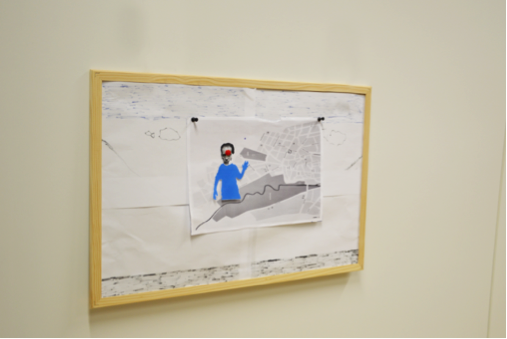
\includegraphics[width=6cm,height=4cm]{Figures/5/paper_board} }}%
    \hfill
    \subfloat[]{{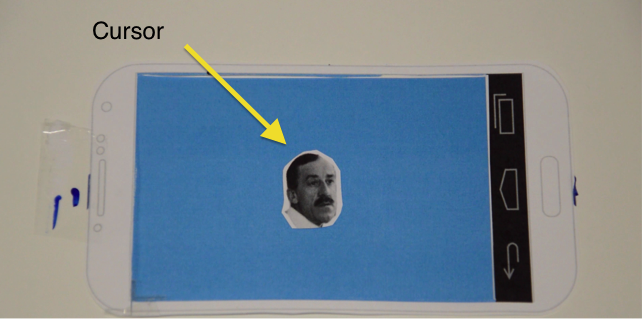
\includegraphics[width=6cm,height=4cm]{Figures/5/mobile_paper} }}%
    \caption{A: Screen paper prototype. B: Mobile paper prototype. }%
    \label{fig:paper_prototype}%
\end{figure}



\subsection{Subjects}
Five participants were invited to experience with the paper prototype.
The participants were from different background, like Media Art, Media architecture and computer science.

\subsection{Location}
Participants were invited in Digital Bauhaus Lab ground floor, where the environment was prepared for the paper prototype interaction.


\subsection{Procedures}
The test subjects will be given basically one task by the interactive advertisement screen and by user body movement their location on the paper screen would be changed and checked for possible interactive object so that the content could be changed and for mobile interaction the subjects will be instructed to think-aloud while interacting with mobile interface so that examiner be able to change content on paper screen.

\begin{figure}[H]
    \centering
    \subfloat[]{{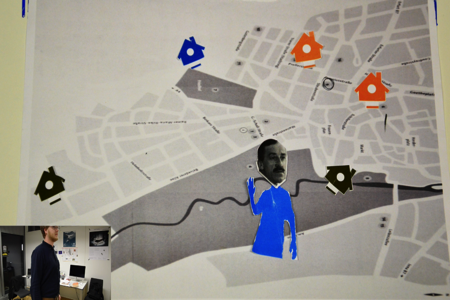
\includegraphics[width=6cm,height=4cm]{Figures/5/body_interaction} }}%
    \hfill
    \subfloat[]{{\includegraphics[width=6cm,height=4cm]{Figures/5/mobile_interactions} }}%
    \caption{A: Body interaction.  B: Mobile Interaction. }%
    \label{fig:Interactive_prototype}%
\end{figure}



\section{Data gathering}
The process of data gathering was as bellow, the methods are designed in a way to fully answer the research questions and the defined hypothesis.


\begin{enumerate}
\item Video Recording \\
Each participant was video recorded for both body and mobile interactions for later observation and analyzing purpose. 

\item Direct observation \\
Participants were observed during the interaction and also asked about what they thought at that moment while interacting. When participants could not perform a task then they were asked exploratory questions on how would they do the task naturally.

\item Think aloud \\
Participants were asked to read their mind while interacting with the prototypes. This helped to understand what they thought about a specific interaction at that moment. 

\item Interviews \\
After both paper prototype interactions were finished, a brief interview was taken to further learn about the interactions they did and get other user comments and feedbacks for the prototypes.
\end{enumerate}


\section{Findings}
The important part for analyzing the data is shaped based on the defined hypothesis at the beginning; the bellow procedure was followed to best answer our open questions and to be able to evaluate both paper prototypes. For interview codings see Appendix \ref{AppendixC}


\subsection{Usability issues}


\subsection{Body Interactions usability}

\begin{enumerate}
\item Confusions 

\begin{enumerate}
\item  Participant was confused of how should to walk, because it felt that there is not enough space. 
\item  User thought that if he/she moves to the location names or the icons, someone would guide her.
\item  User was confused on the new character photo labeled on the top of his silhouette; he thought that the new character is trying to interact with his silhouette. ``\emph{Is it like people approaching you and say hi and hello, and then ask me if I can visit his places}''
\item  He did not know his places (the character’s places).
\item  Could not understood the word move or walk, he taught that it is not applicable at the moment.
\item  Raise one hand to see if the blue reacts or not.
\item  Did not recognize the person.
\item  Did not understand the task.
\item  Did not understand what is the blue person.
\item  Asked question about who is the face, he did not know it.

\end{enumerate}

\item Frustrations
\begin{enumerate}
\item  Entering IP address.
\item  When the wrong house was explored, and she said ``\emph{(Ohh No)}''.
\item  Waiting for the houses to load on the screen.
\end{enumerate}

\item Mistakes
\begin{enumerate}
\item  Entered to the wrong location.
\item  Did not know how to navigate to the places. Even he was told that the silhouette is his body.
\item  Navigating the silhouette was a problem for her; she wanted to go on top of the map in the screen but physically moved back. And after seeing the reaction she corrected herself.
\end{enumerate}

\item Comments
\begin{enumerate}

\item   There should be very clear instruction in the application on what to do, what it is about and how to do it.
\item   I did not understand the person; maybe do not use it anymore.


\end{enumerate}
\end{enumerate}


\subsection{Mobile usability}
The bellow chart lists all the possible issues with mobile interaction.

\begin{enumerate}

\item Confusions
\begin{enumerate}
\item  The idea of the application was not clear for her because she taught that the mobile application could be used when she goes out in the city. But later she found out that the screen and mobile are both of them used at a place.
\item  Navigation was a big confusion for him; he was touching the character on the mobile screen.
\item  The turning phone as shown in arrow, since she could not turn the phone.
\item  Did not understood what happened after the interaction was over. She did not read the texts or she did not understand why those were about.
\item  The face in the mobile.
\end{enumerate}

\item Frustrations
\begin{enumerate}
\item  Visiting to all locations to finish the interaction.
\item  Not enough things when visiting to a location.
\item  She felt frustrated when visiting the wrong location and find the right location.
\item  He had to re-login because he accidently pressed cancel button.
\item  Visited to the wrong location.
\item  Waiting for the houses to load on the screen.
\end{enumerate}

\item Mistakes
\begin{enumerate}
\item  Did not understand to scan QR code.
\item  Took longer time to use the phone prototype. 
\item  Did not understand to rotate the mobile. As the instructions were shown on the phone.
\item  Took longer time to navigate the person on the screen.
\item  She tried to continue without putting any name in the form.
\item  Did not understand how to turn the phone, she touched the arrow on the screen many times. But nothing happened. Later she knew to turn the phone, but did not do it because she thought that the paper prototype should not be moved from its place.
\item  Could not navigate the person on the screen.
\item  Entered the wrong IP address, but then changed his mind and scanned the QR code.
\item  Accidently pressed cancel.
\end{enumerate}

\item Comments
\begin{enumerate}
\item  There is no enough information about the locations; it would be good to show a short description of the place.
\item  There could be like choices like when the opening time is for these locations.
\item  How far are they from my current location, the distance?
\item  View the transport possibilities to the selected locations.
\item  It would be good to have more information about the locations.
\item  And I would like to see the entire map on the phone too.
\item  I like to see some more information in my phone.
\item  There should be more guides when I use the phone, like there should be like Samsung, when you turn it on for the first time, it shows how to use what or it should have a finger picture to swipe on the face.
\end{enumerate}

\end{enumerate}

This chart was created to list all the possible, mistakes, misunderstandings and confusions for each of the interactions carried by participants, these lists were categorized under usability problem. This error chart was made during video observations, flow of the tasks were observed and also the words they used during interaction from which confusion, frustration and misunderstandings events were recorded. 

Looking through all the usability problem chart of each participant the bellow single chart is being created, each category is separately listed with the possible problems.


\subsection{Hypothesis decisions}

The hypothesis those were defined in the design study, from which some of them are accepted and rejected based on the above findings. 

\subsubsection{Body Interaction}
\begin{itemize}
\item H1: Users understand and react to the Call-to-Action approach.\\ 
\textbf{[Accepted]}\\
All of the participants understood call-to-action and reacted to it quickly as soon they read it.

\item H2: Users recognizes the character assigned to them.\\ 
\textbf{[Rejected]}\\
All the participants did not understand the character which was assigned to them, This happens when the participants do not have background to the related history that should know the character, It would be better to use someone who is very famous and is known to most of the population and different cultures, using very specific character is a bad idea. Users gets confused. At one occasion even an architect student who must know that face, but unfortunately did not recognized him. 

\item H3: Users understands the tasks assigned to them.  \\ 
\textbf{[Rejected]}\\
Most users did not understand the task in the sense of the defined character, but they did understand that they should walk and explore locations.

\item H4: Users can explore locations by moving their body in physical space. \\ 
\textbf{[Accepted]}\\
As soon they understand that the silhouette is them and projected on the screen, then they did the task by moving them selves physically, except one participant who did not understand until the observer gave him hint to move his self physically in right or left.

\item H5: Application raises alerts to specific user actions.   \\ 
\textbf{[Rejected]}\\
The application did not raised error for user?s specific interactions like if the user was out of the screen or very close to the screen. Most of the participants raised their hand up, or turned around, there was no alerts for the participants.

\item H6: Application motivates participants to continue playing. \\ 
\textbf{[Rejected]}\\
When the users explored the first location, they were excited and tried to see the other places, but all the locations action was predictable by the participants and nothing new was happening, participants expected more from their interactions to be more excited to play the whole game. They did finish the game because they were told so.

\end{itemize}


\subsubsection {Mobile Interaction}
\begin{itemize}
\item H1: Users understand the Access Information shown on the board. \\ 
\textbf{[Accepted]}\\
The participants were not shown the phone prototype at first, they were only shown the display and were asked to react based on the messages or what ever the users comprehend, after reading the Access information they asked for the phone prototype and then the phone prototype was shown to them to interact.

\item H2: Users open the controller website by scanning QR-Code. \\ 
\textbf{[Accepted]}\\
Four of the participants understood the use of QR-code and from which two of them scanned it and other two typed the IP address, and one participant did not understood the use of QR-code.

\item H3: Webpage application produces alerts with in correct user input.\\ 
\textbf{[Rejected]}\\
The webpage did not produce error at many occasions while filling the form like, what happens when cancel button is pressed, or when the game finishes the application does not alert user to replay or leave webpage.

\item H4: Users rotate the mobile phone to start game.\\ 
\textbf{[Rejected]}\\
Only two of the participants rotated the phone but the rest of the participants tapped on the icon and tried to rotate the icon in the screen instead rotating the whole phone.

\item H5: Users understand the task.\\ 
\textbf{[Rejected]}\\
This happened because all of the participants did not recognized the face and did not know where are his locations.

\item H6: Users can navigate the character by moving the face in mobile.\\ 
\textbf{[Rejected]}\\
Four of the participants touched and tapped the face shown on the mobile phone many times, they expected that something will happen after they touch the character like a dropdown list would appear to edit it, but one of the users drag it and saw the reaction on the screen.

\item H7: Screen application produces alerts for incorrect location.\\ 
\textbf{[Accepted]}\\
The incorrect locations that were explored by the participants were given an alert message.
\end{itemize}



\newpage
\section{Conclusions}

Evaluation of low-fidelity prototype of advertisement was very helpful to understand possible design problems and interactions that could have been a headache if had identified at high-fidelity version. 

First, the body interaction was easily understood by most of the participants, this type of interaction is more natural and can be done by any kind of participant without having any technical expertise. Two most important interactions in this technique was the call-to-action which approached participants to come near to the screen and other was to explore the locations using their body position in physical space. This low-fidelity usability testing suggests bringing changes for the next high-fidelity version of the advertisement. The changes would be to remove the character assigning for individuals, improving alert messages for different user actions, improving task description and integrating features to increase interest rate for participants to be engaged with the advertisement.

Second, participants also appreciated the mobile interaction, but they were not so convinced for the usage because of many issues like logging in web application first, then navigating the face character. There was no clear instructions for how to navigate the character, and what will happen if there are many participants playing at the same time, where all of the participant would have the same face and they would get confused that which one is being controlled by their controller and lastly, it was unclear that what happens in web application when the interaction is over. This usability testing helped us to identify the mention usability problems and would bring changes for the new high fidelity version that would solve the current issues.

Third, The advertisement text, which was shown at the end of interaction, did not brought user?s attention, it would be better to make a short video for the next prototype that could bring users attention to see the advertisement. After the video advertisement gets over the attraction phase starts again.

Finally, all hypotheses that were accepted or reject will be taken in to account from which new decisions for the high fidelity version will be taken, this version will overcome all the issues discovered until this stage. Participant?s recommendations and feedbacks have also much value and would be considered in the development phase.









% Chapte 7
\chapter{Advertisement application} % Main chapter title

\label{Chapter7} % For referencing the chapter elsewhere, use \ref{Chapter1} 
\newpage
.
\newpage

\section{Introduction}
The use of technology in advertisement plays a major role in advertisement industries. It would have been much difficult to reach to customers without technologies, and technology enhances the two-way communication with the client and the customers. The companies can now easily express their thoughts and vision to their customers with the help of the latest technologies. Advertisements are everywhere, in websites, in your smartphone, in television and radio. Since the last decade, it is more common to see advertisements on the streets, in supermarkets, airports and any place of public gatherings.
So, for every context or settings there are different kinds of technology that are being used to make the advertisement more appropriate. When it comes to interactive advertisement, the use of right technology plays another major role in terms of usability and understandability. Interactive advertisements on websites are usually interactive using keyboard and mouse, whereas in smartphone, advertisements use only the capability of the touch or other sensors to make the interaction easy. Interactive advertisements in public spaces have another bunch of technologies that make the interaction usable like using face recognition, body position recognition, hand gesture recognition and also touch sensors, proximity sensors and much more.


This chapter explains all the technical aspects of the advertisements system that were developed during the thesis work for attracting attention and the main advertisement application. It discusses what technologies and hardware have been used and what algorithm and methods were implemented to accomplish the goals. Besides the technical details it describes the interaction design of interactive advertisement.



\iffalse
\section{Attracting attention Application}
The goal of attraction attention was to develop systems that could attract the attention of the passersby, in which three different applications were developed and later compared.

\subsection{Requirement gathering}
The below are the required elements used for the applications.


\subsubsection{Hardware requirement}

\begin{itemize}
\item \textbf{Microsoft Kinect Camera} \cite{Kinect} \\
This is one of the most used camera in public context a lot, this camera can track up to seven user's position (X, Y, Z) in real time; it is capable of recognizing hand gesture and even can track facial movements. The camera does not work well when it is exposed in sunlight, which makes it ideal for indoor use only. In our experiment Microsoft Xbox 360 Kinect camera was used, The Kinect camera should be used with an extra adapter in order to connect it to computer. 
\item \textbf{Computer} \\
A normal laptop was used with Core i7 2.7 Ghz processor, and 4 GB RAM and USB of 2.0 version.
If you want to use Xbox Kinect One Kinect then the computer should support USB version 3.0.
The laptop was connected to the University monitor via mini display port.

\end{itemize}


\subsubsection{Software requirement}
The software can run in any operating system except because of the processing programming language. In experiment mac OSX operating system was used with below library and processing version.
\begin{itemize}
\item Processing v2.2.2 or higher version.
\item SimpleOpenNI library for Processing \cite{simpleopenni}
\item 32bit JRE (Java Runtime Environment) v1.8 or higher.
\end{itemize}


\subsection{Following eye application}
The name is given \emph{Following eye} because the application shows eyes for each individual when pass from the front of the screen and those eyes follow the person where they walk. The interaction works with the Kinect camera that provides each individual positions.
Explore the attached CD for the source code.

\subsection{Firework application}
This application also uses kinect camera to track user position and renders a firework animation for each person.
The fireworks are created with using random number of circls (balls) with random colors and sizes, the circles burst from the person's location and spreads to random directions with a high speed and slows down at the end. One part of the application's code is freely taken from openprocessing community that could generate random firework bubbles.
For more detail please check the CD for source code.
\fi


\section{Advertisement Applications}
In this section the main advertisement applications are being discussed.
According to the plane there was a need to develop three-advertisement application (non-interactive, body interactive and mobile interactive), which had the same functionality but were different in terms of interactivity and control.

The advertisement application was designed to show important places of \emph{Bauhaus} that are included in \emph{Bauhaus-Walk} tour, the pictures of these places are attached on the Weimar map with a name at top and a small description below of the picture frame. This technique helps participants to build a relationship of the locations and the map. Only five locations are randomly chosen by the software to be shown on the map, each animates one after another and. When all the locations are explored then the advertisement video is played and the application repeats itself again.


\subsection{Non-Interactive application}
It can be understood from the name, passersby have no control over the flow of this advertisement, but it triggers automatically. It automates through whole three hierarchical levels of interfaces, (1) Initial interface, (2) Map interface, and (3) the advertisement video interface. All the interfaces have a fixed time in which it will switch from one to another. Watch this Video\footnote{Non-interactive advertisement: \url{https://www.youtube.com/watch?v=ZLszzfbZJgI}, last accessed 1 july 2016} to see the flow of the interfaces.


\begin{figure}[H]
    \centering
    \includegraphics[width=0.8\textwidth,height=30mm]{Figures/7/application_flow}
    \caption{Interface flow}%
    \label{fig:InterfaceFlow}%
\end{figure}

\begin{enumerate}

\item Initial Interface: \\
The initial interface of the advertisement shows the \emph{Gropius walter} room, the \emph{Bauhaus-Walk} name on the upper left side, and the Bauhaus University logo at the bottom right corner.

\begin{figure}[H]
    \centering
    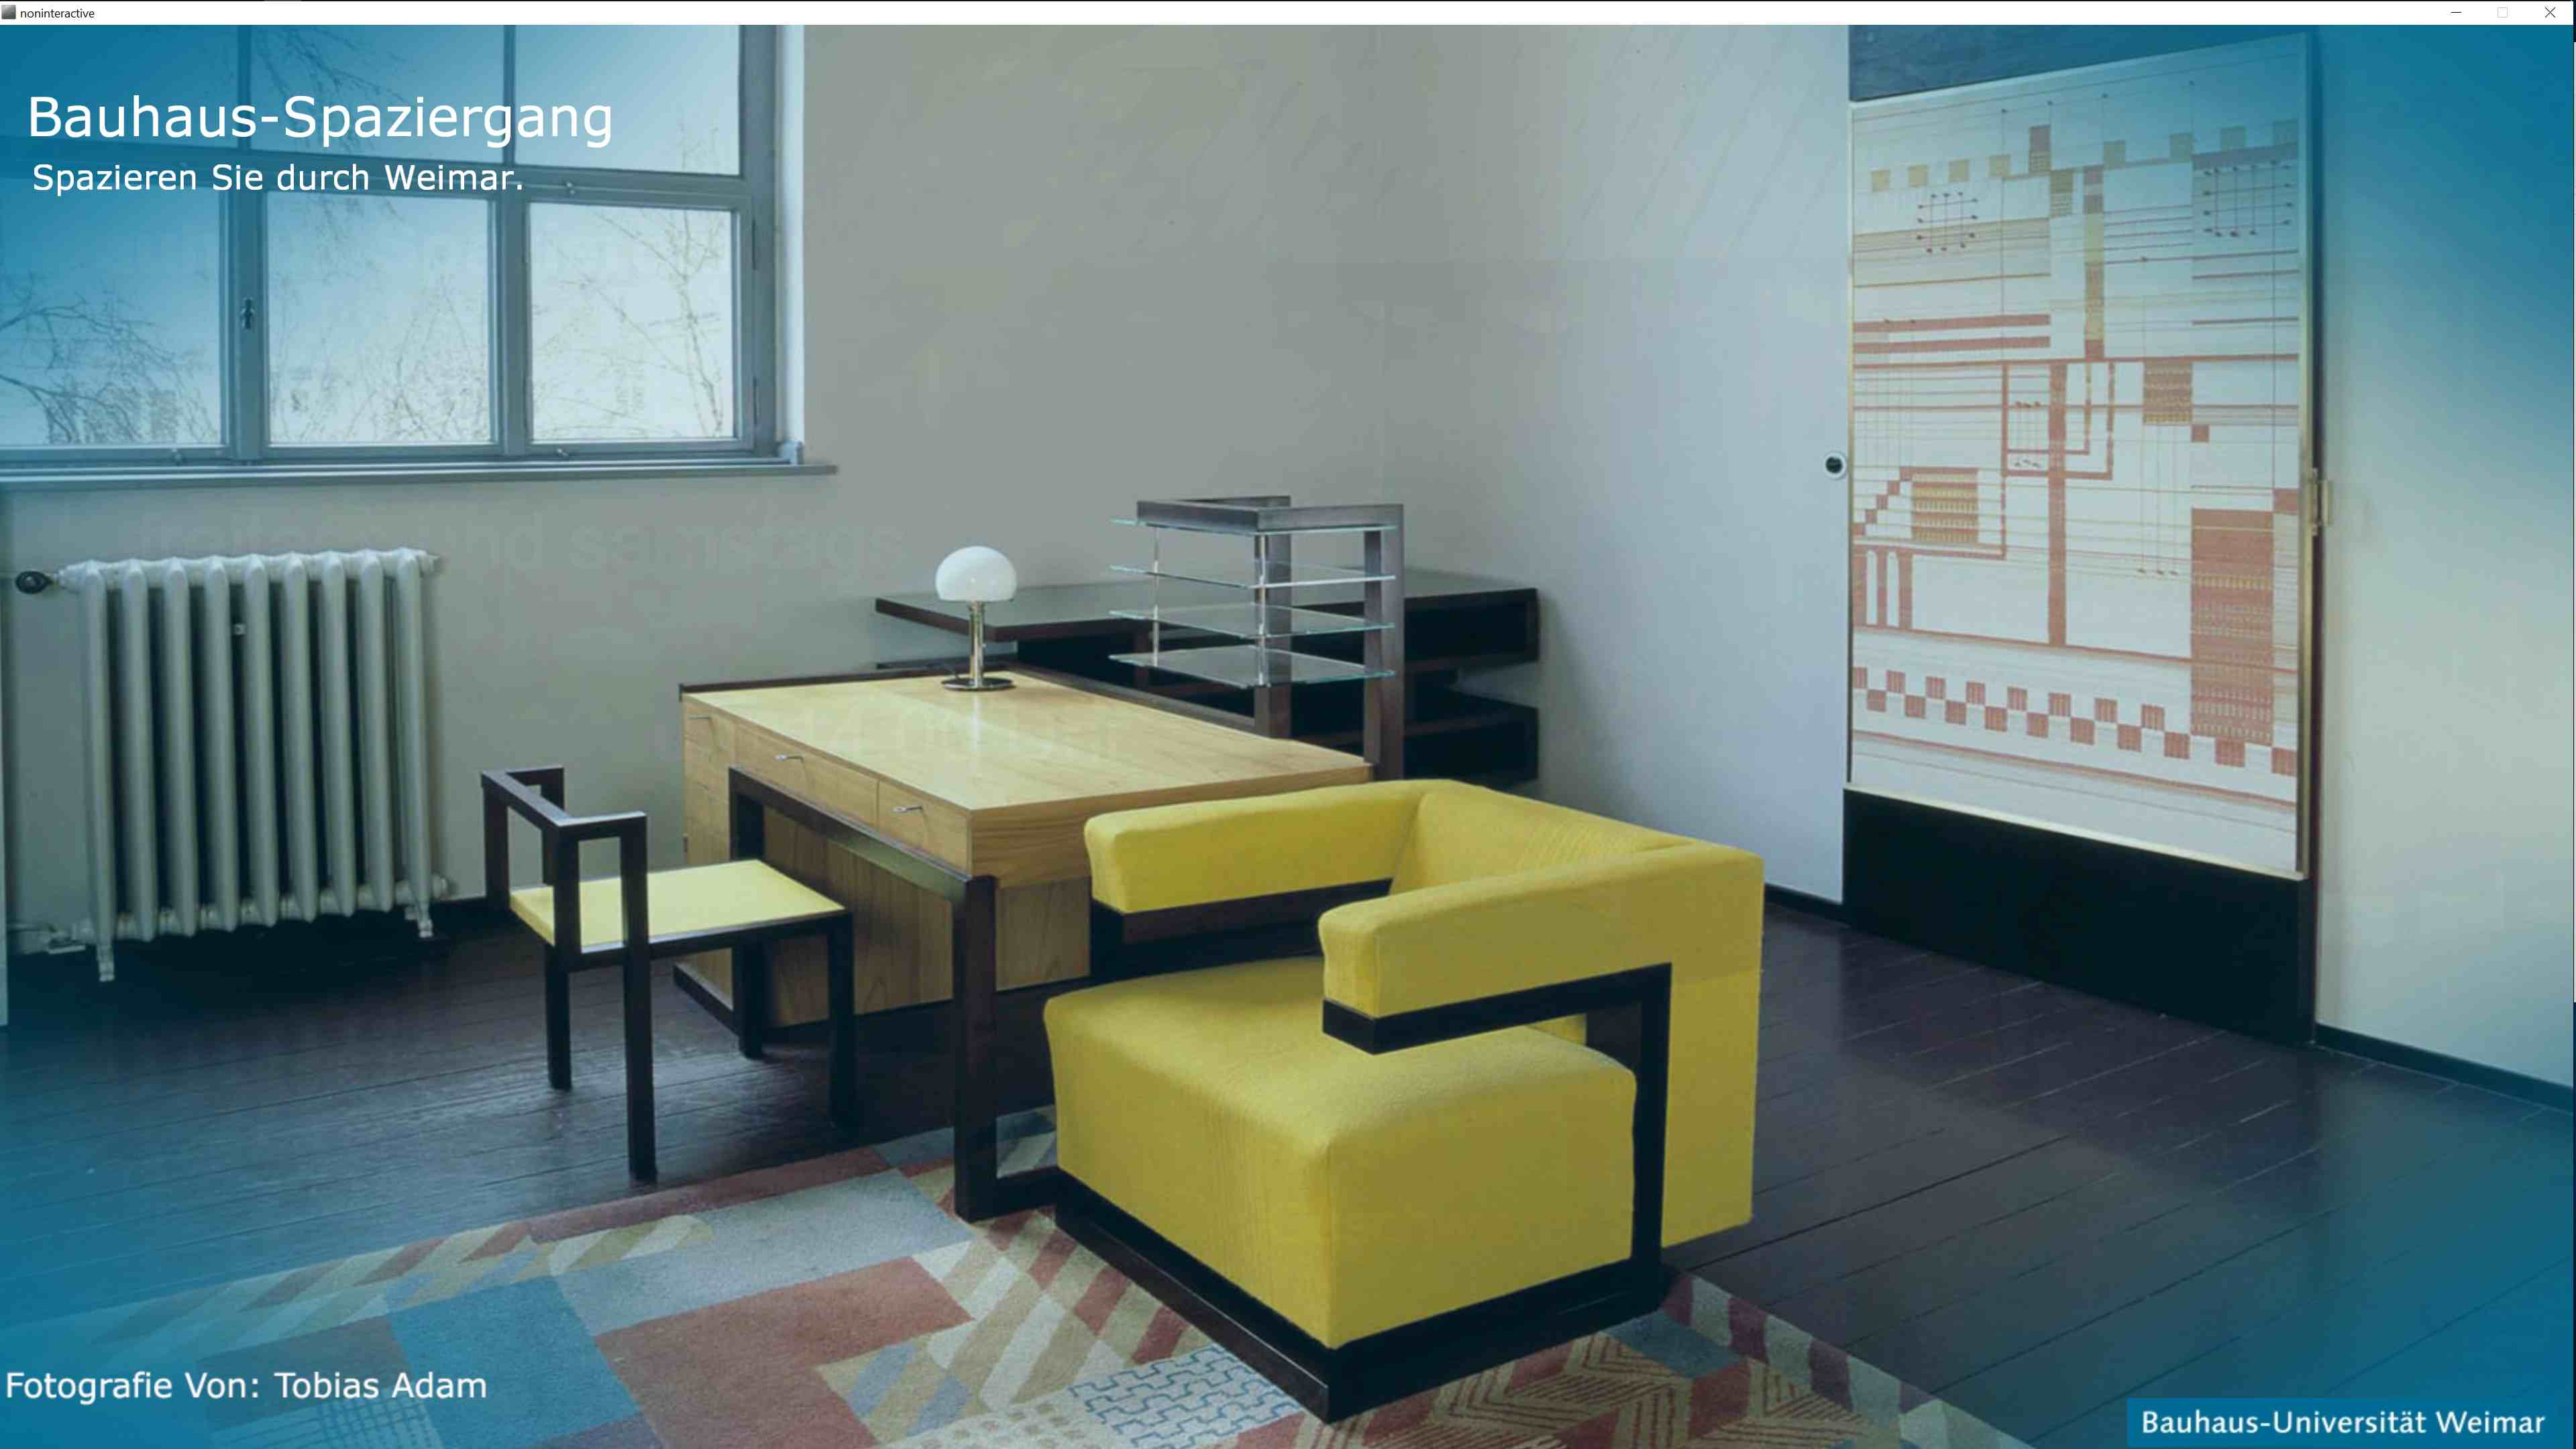
\includegraphics[width=100mm,height=60mm]{Figures/7/initialpage}
    \caption{Initial Interface}%
    \label{fig:adInitialpage}%
\end{figure}

\item Map Interface: \\
This is the city map of Weimar that has some interest regions shown on the top of the map. Those regions are blinking to signal the users.

\begin{figure}[H]
    \centering
    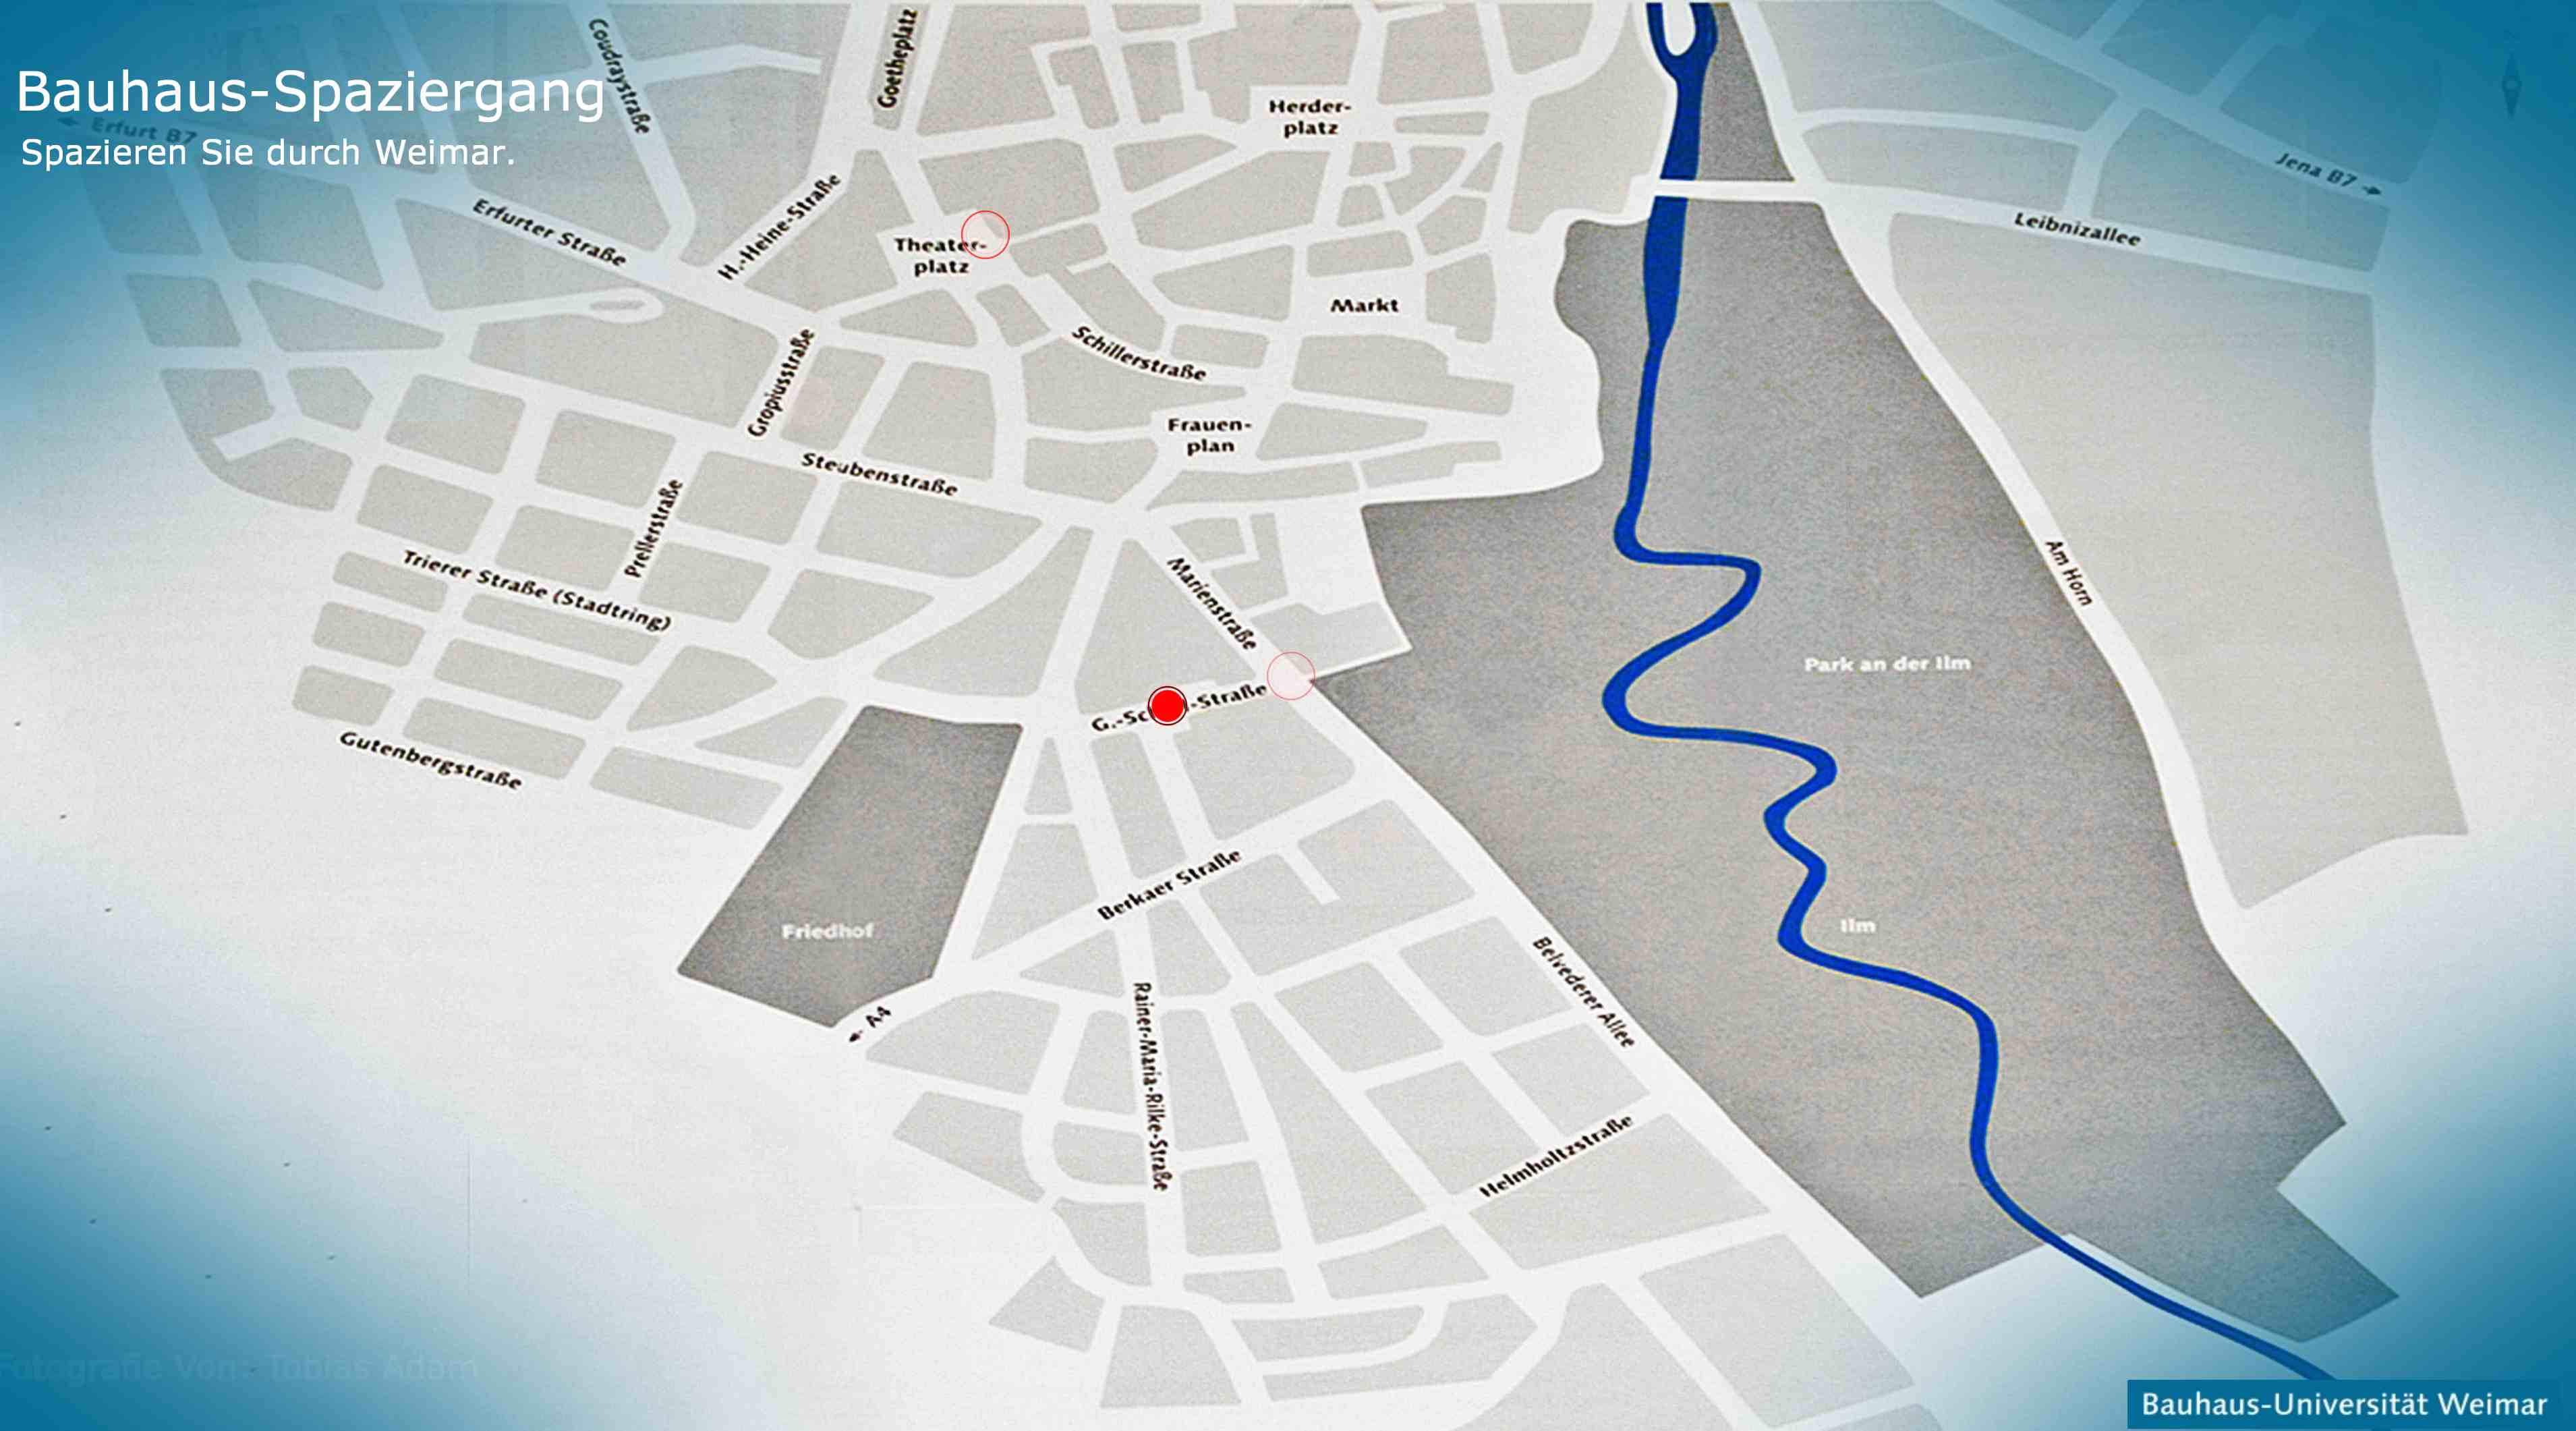
\includegraphics[width=100mm,height=60mm]{Figures/7/map}
    \caption{Map Interface}%
    \label{fig:adSecondpage1}%
\end{figure}

The location pictures are animated randomly and they are first enlarged, and then resized backed to fit on the map region.
\begin{figure}[H]
    \centering
    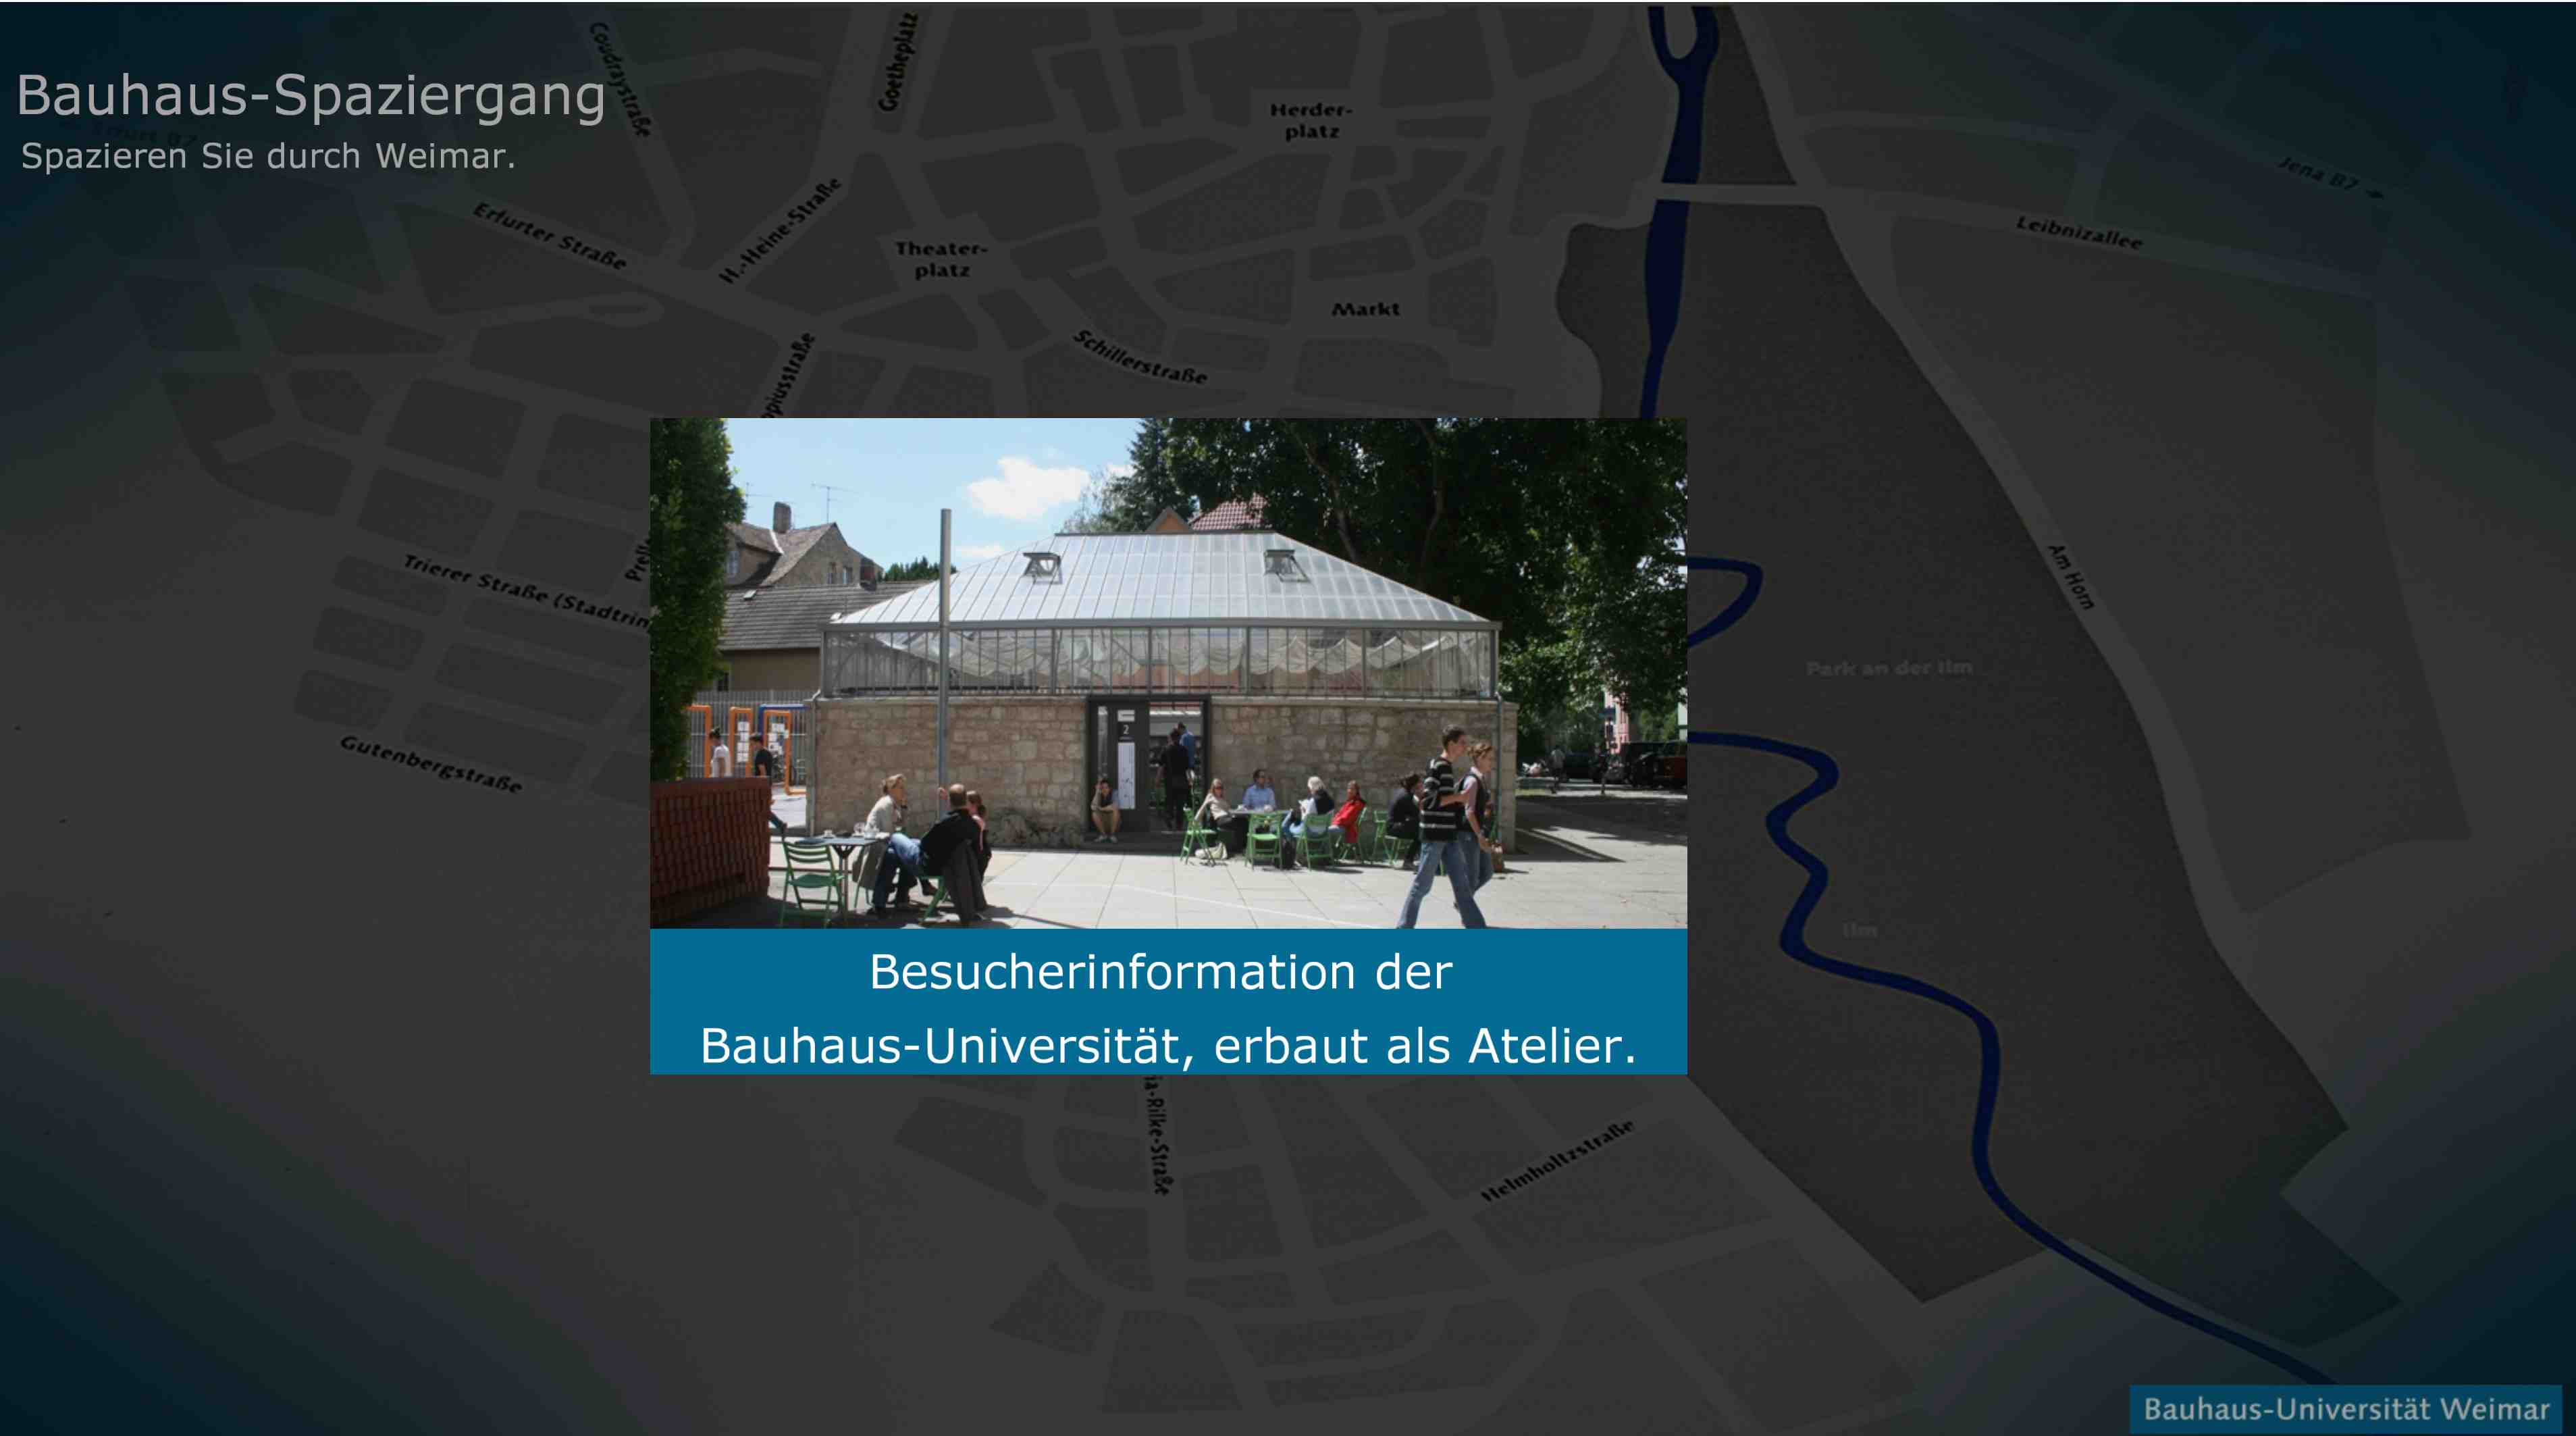
\includegraphics[width=100mm,height=60mm]{Figures/7/enlarged_pic}
    \caption{Enlarged picture}%
    \label{fig:adSecondpage2}%
\end{figure}

The resized pictures on the map looks like below. 
\begin{figure}[H]
    \centering
    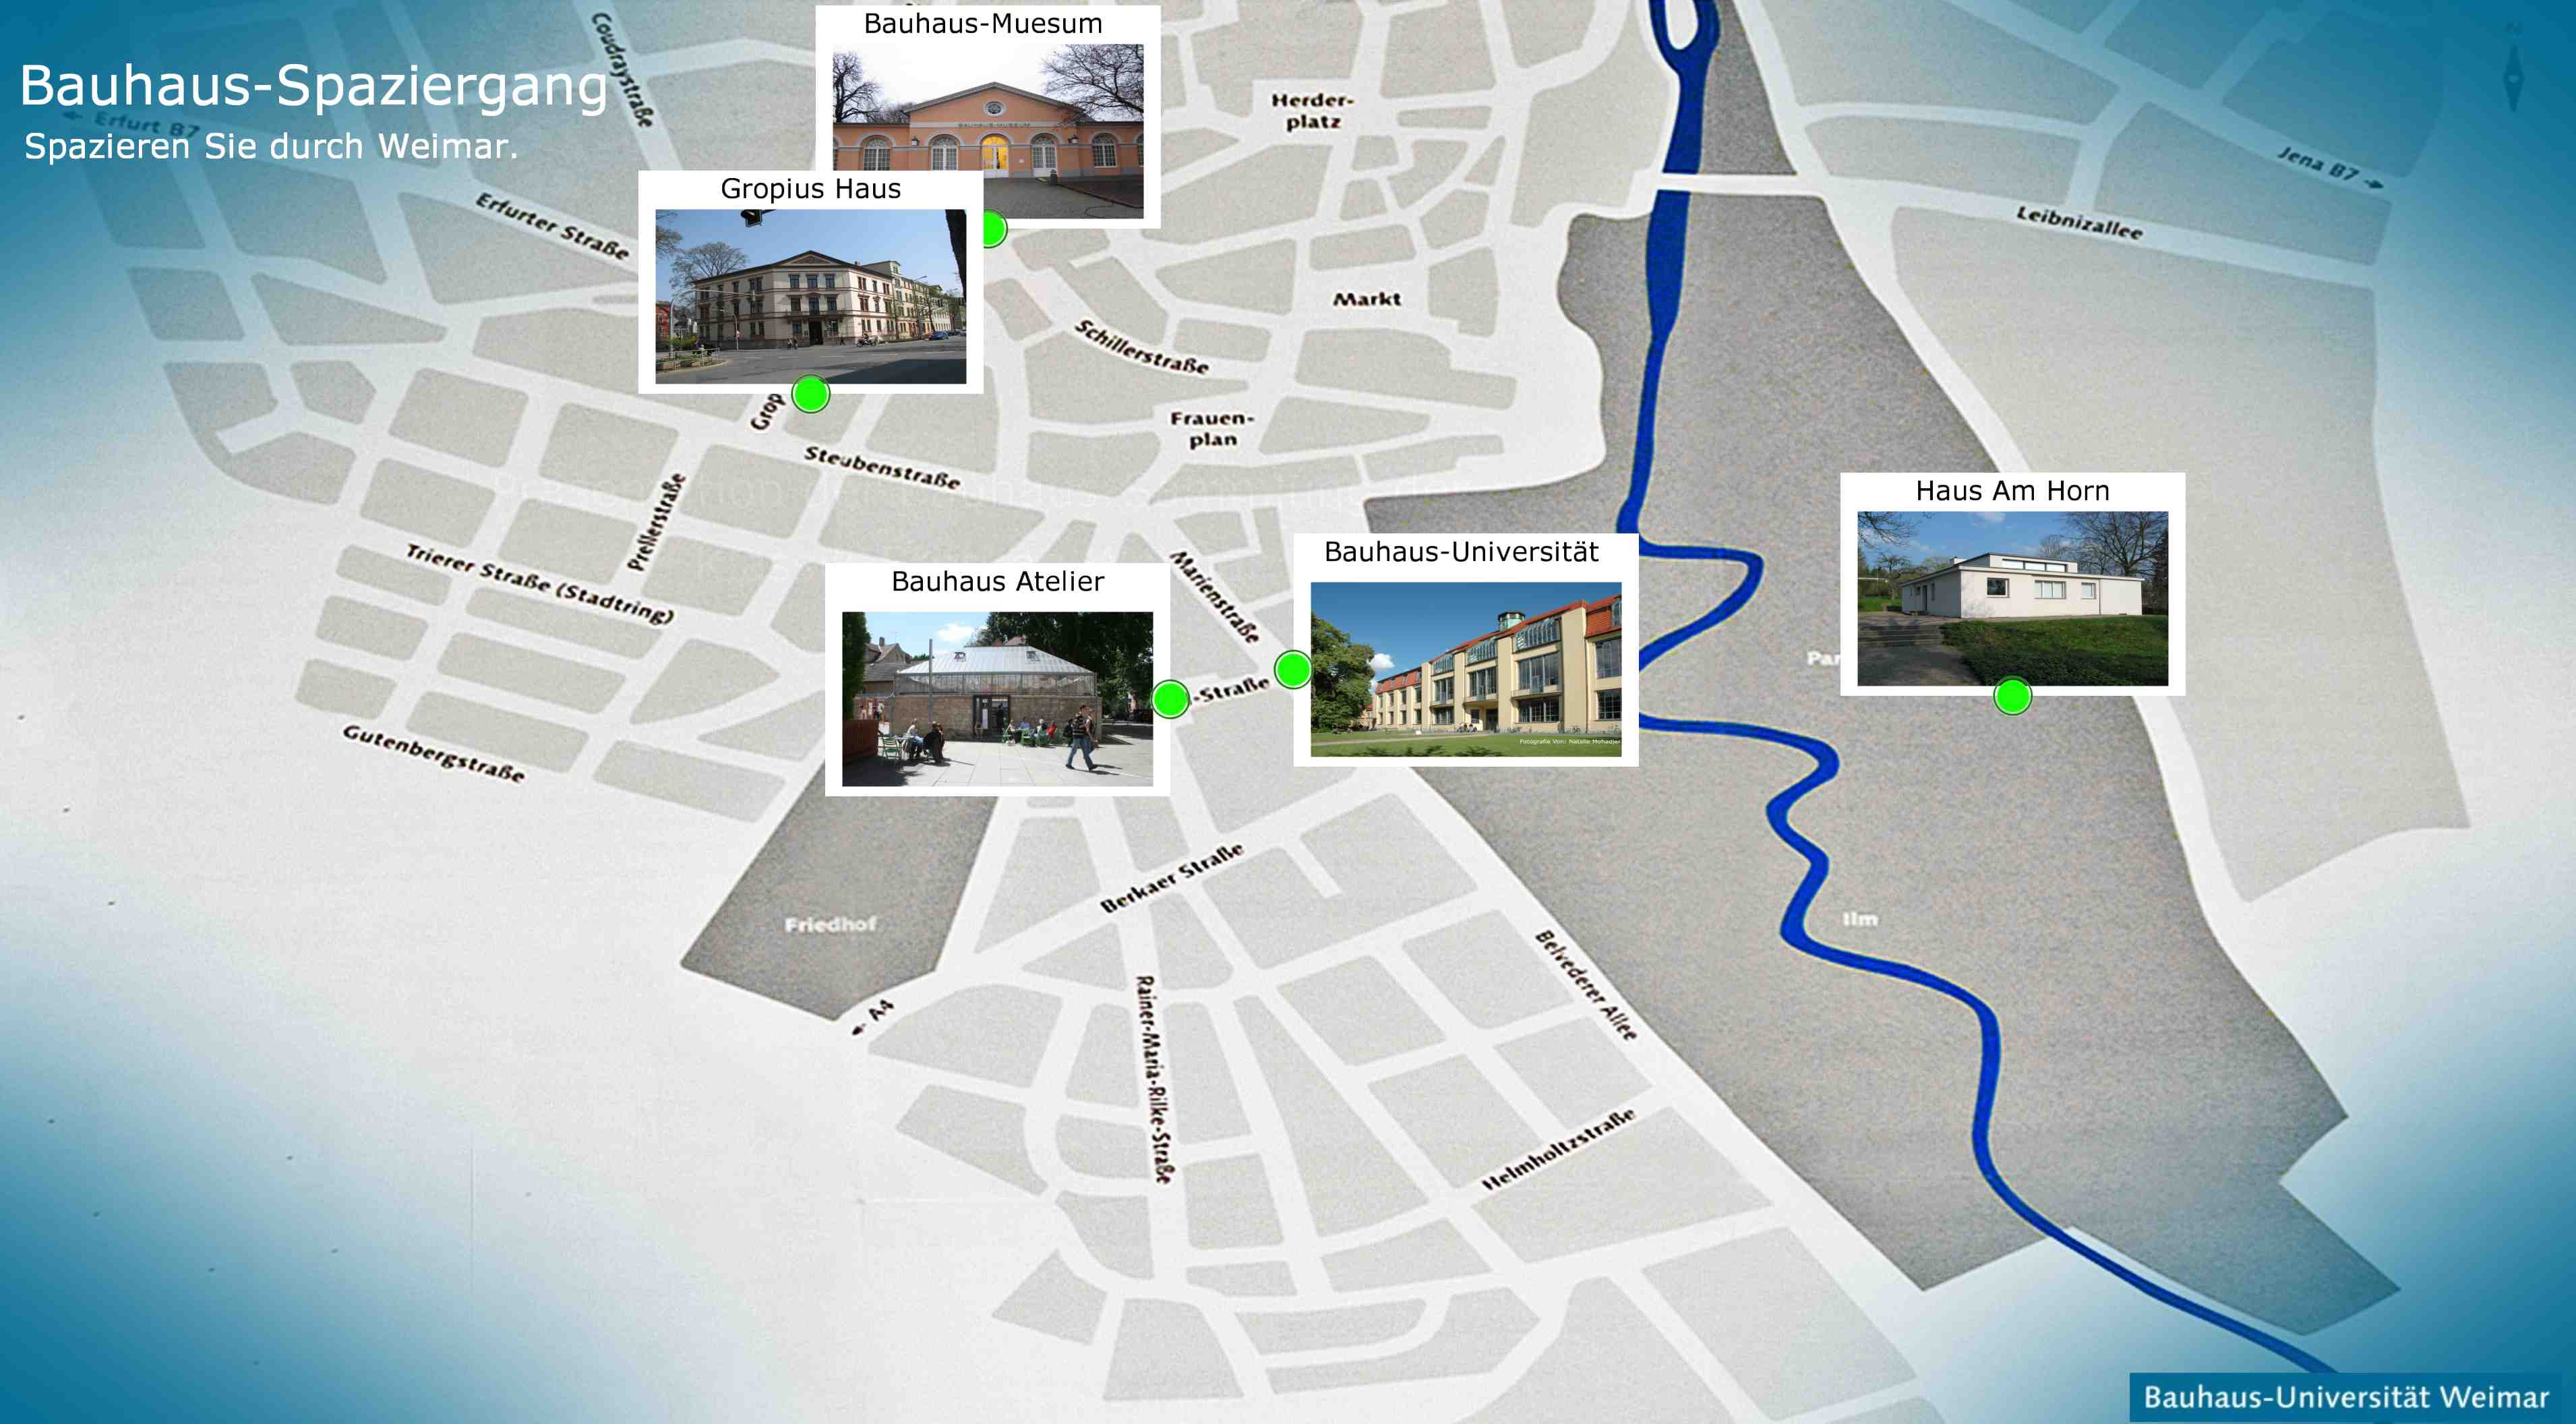
\includegraphics[width=100mm,height=60mm]{Figures/7/map_pictures}
    \caption{Pictures on the map}%
    \label{fig:adSecondpage3}%
\end{figure}

\item Advertisement video:\\
In this interface the video is being played, this picture is a screenshot of one of the frames of the video.
\begin{figure}[H]
    \centering
    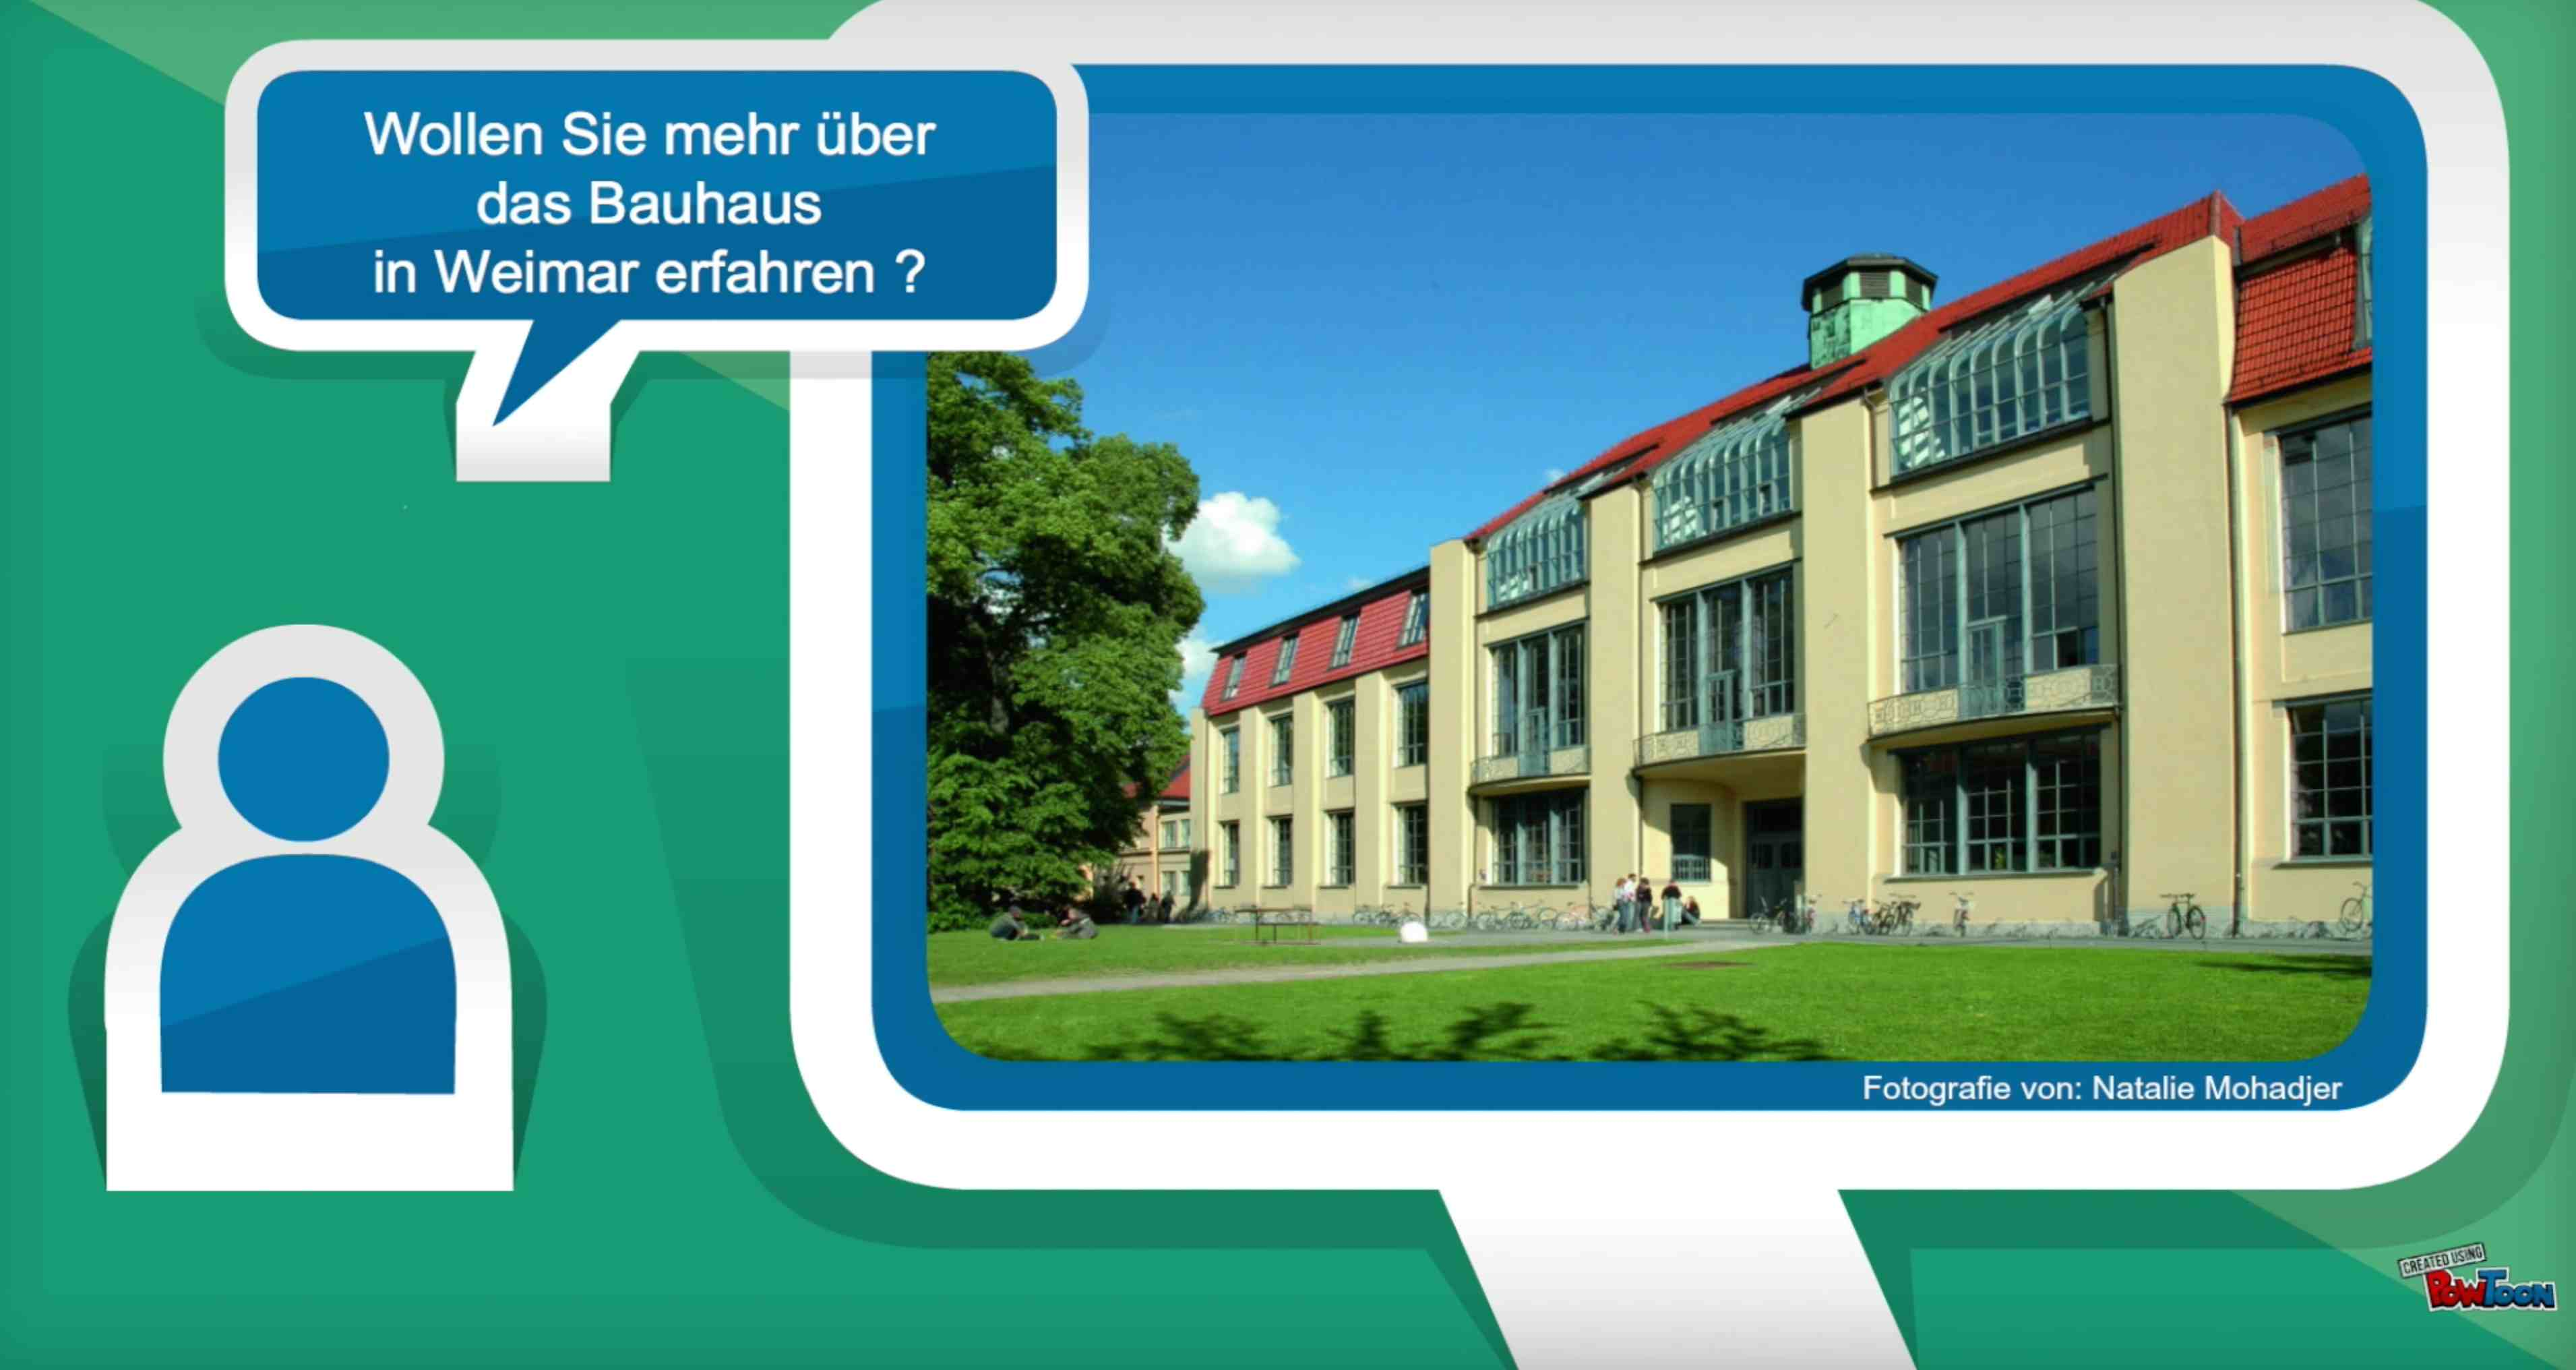
\includegraphics[width=100mm,height=60mm]{Figures/7/ad_first}
    \caption{Advertisement video}%
    \label{fig:adthirdpage1}%
\end{figure}

This is the last frame of the video that shows information about how and where to join the Bauhaus Walk.

\begin{figure}[H]
    \centering
    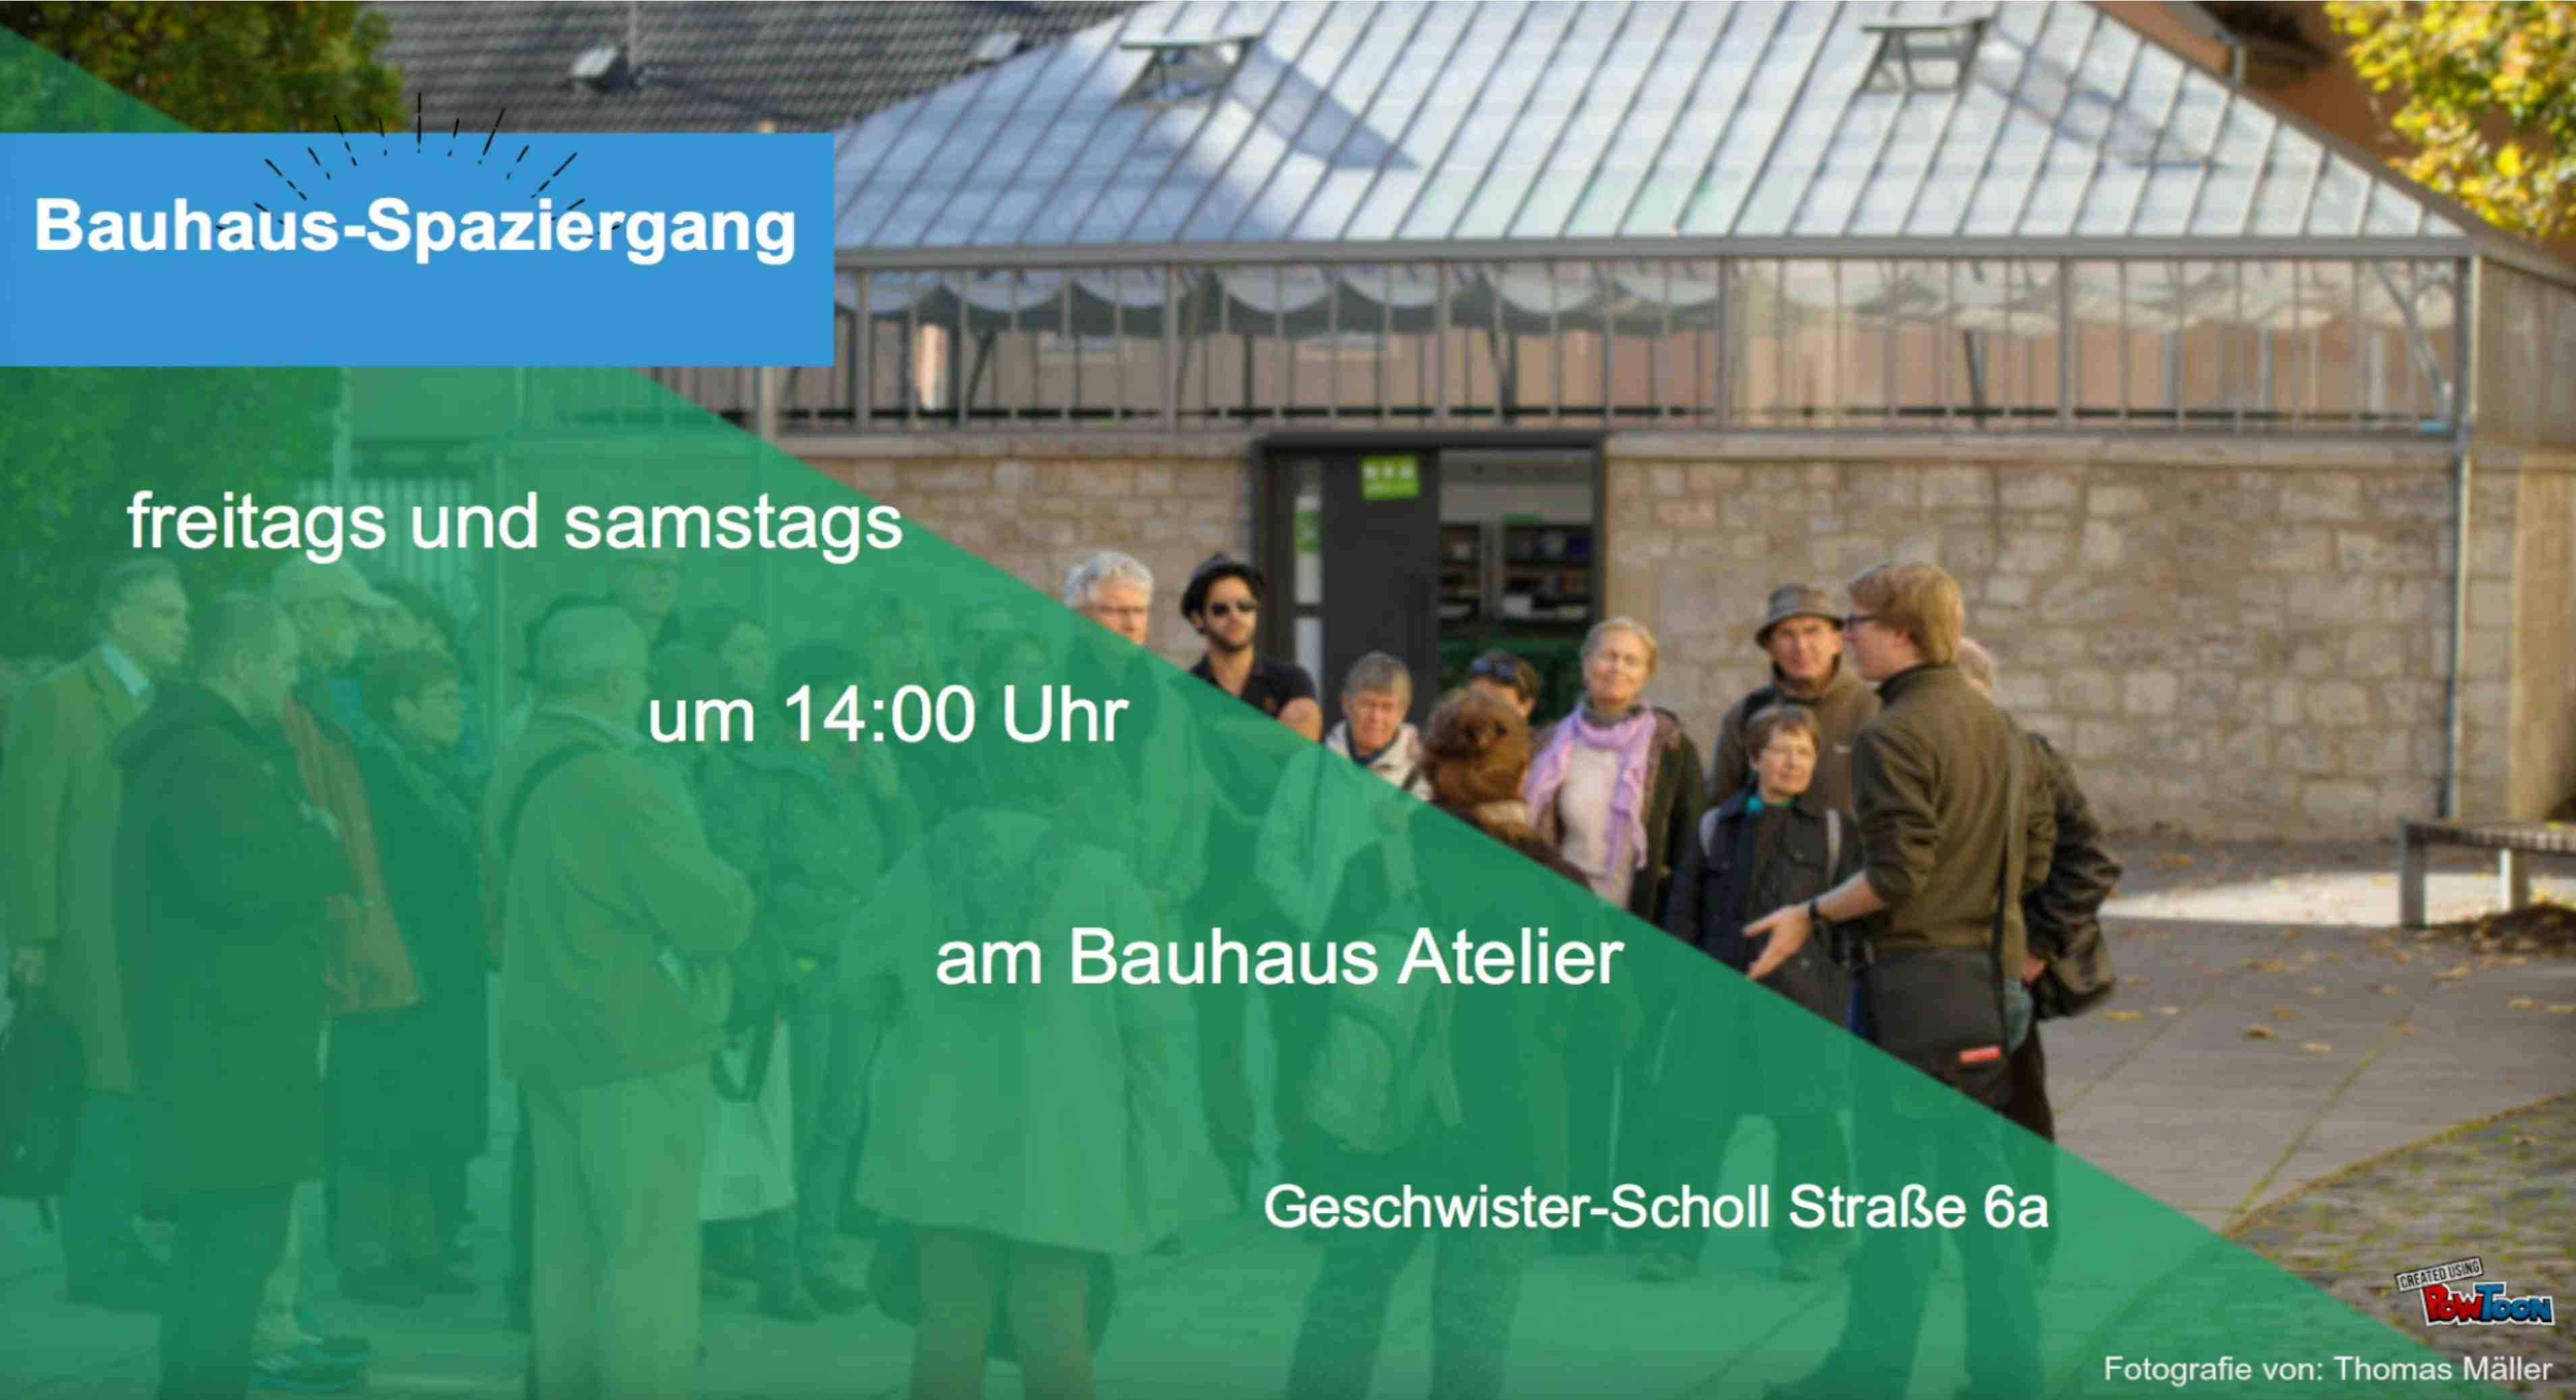
\includegraphics[width=100mm,height=60mm]{Figures/7/ad_last}
    \caption{Advertisement video last frame}%
    \label{fig:adthirdpage2}%
\end{figure}

The advertisement video was created in PowToon\footnote{PowToon: \url{https://www.powtoon.com/index/?gclid=CJqSqrf5l80CFesV0wod1u8IEQ&edgetrackerid=10083804111572}, last accessed 5 jun 2016} with a free version account, visit this video\footnote{Advertisement Video:  \url{https://www.youtube.com/watch?v=-y1Dbz6E6bU&feature=youtu.be}, last accessed 5 jun 2016} that shows the advertisement video. See Appendix \ref{app:fileandfolders} for video path in DVD.

To see the full the non-interactive advertisement flow of the interfaces and its animations visit this video\footnote{Non-interactive Ad: \url{https://www.youtube.com/watch?v=ZLszzfbZJgI}, last accessed: 5 Jun 2016}.See Appendix \ref{app:fileandfolders} for video path in DVD.


\end{enumerate}

\iffalse
\subsection{Hardware setup}
The below setup is the hardware setup for the advertisement. The same setup is used for all three weeks.

\begin{figure}[H]
    \centering
    \includegraphics[width=100mm,height=70mm]{Figures/7/Physical_setup}
    \caption{Hardware setup}%
    \label{fig:hardwaresetup}%
\end{figure}


\hilight{put the picture of the screen here}

\begin{figure}[H]
    \centering
    \includegraphics[width=100mm,height=70mm]{Figures/7/Physical_setup}
    \caption{Picture}%
    \label{fig:hardwaresetup}%
\end{figure}



\subsubsection{Flowchart Diagram}

\begin{figure}[H]
    \centering
    \includegraphics[width=100mm,height=90mm]{Figures/7/Non-interactive/flow_chart_diagram}
    \caption{Non-interactive Flowchart diagram}%
    \label{fig:non_inter_flowchart}%
\end{figure}
\fi


\subsection{Body Interactive application}
As discussed earlier, there are three interfaces or phases (initial interface, map interface and advertisement video) of the application, and in body interaction the same interfaces are used, but two of them are interactive. The first two interfaces are interactive and allow participants to interact with using their body like exploring the interest points on the map by moving physically (forward, backward, right and left) in front of the screen. The last interface shows advertisement video, which is not interactive.  All the interfaces are explained in the following sections.

\begin{enumerate}

\item Initial Interface (\emph{Call-to-Action}) : \\
This interface is basically the same interface as the non-interactive but with a difference. It projects passersby silhouette on the interface, this interface is also called \emph{Call-to-Action} interface because it calls passersby to interact with the screen. As can be seen in the below picture, there is someone standing in front of the screen and the interface calls him to come near. This interface also has alert messages on the top right corner of screen that alerts the participant if they move away from the camera range. In this example a second person had got untracked from the camera and the system has shown that message to raise his hand to be tracked again.

\begin{figure}[H]
    \centering
    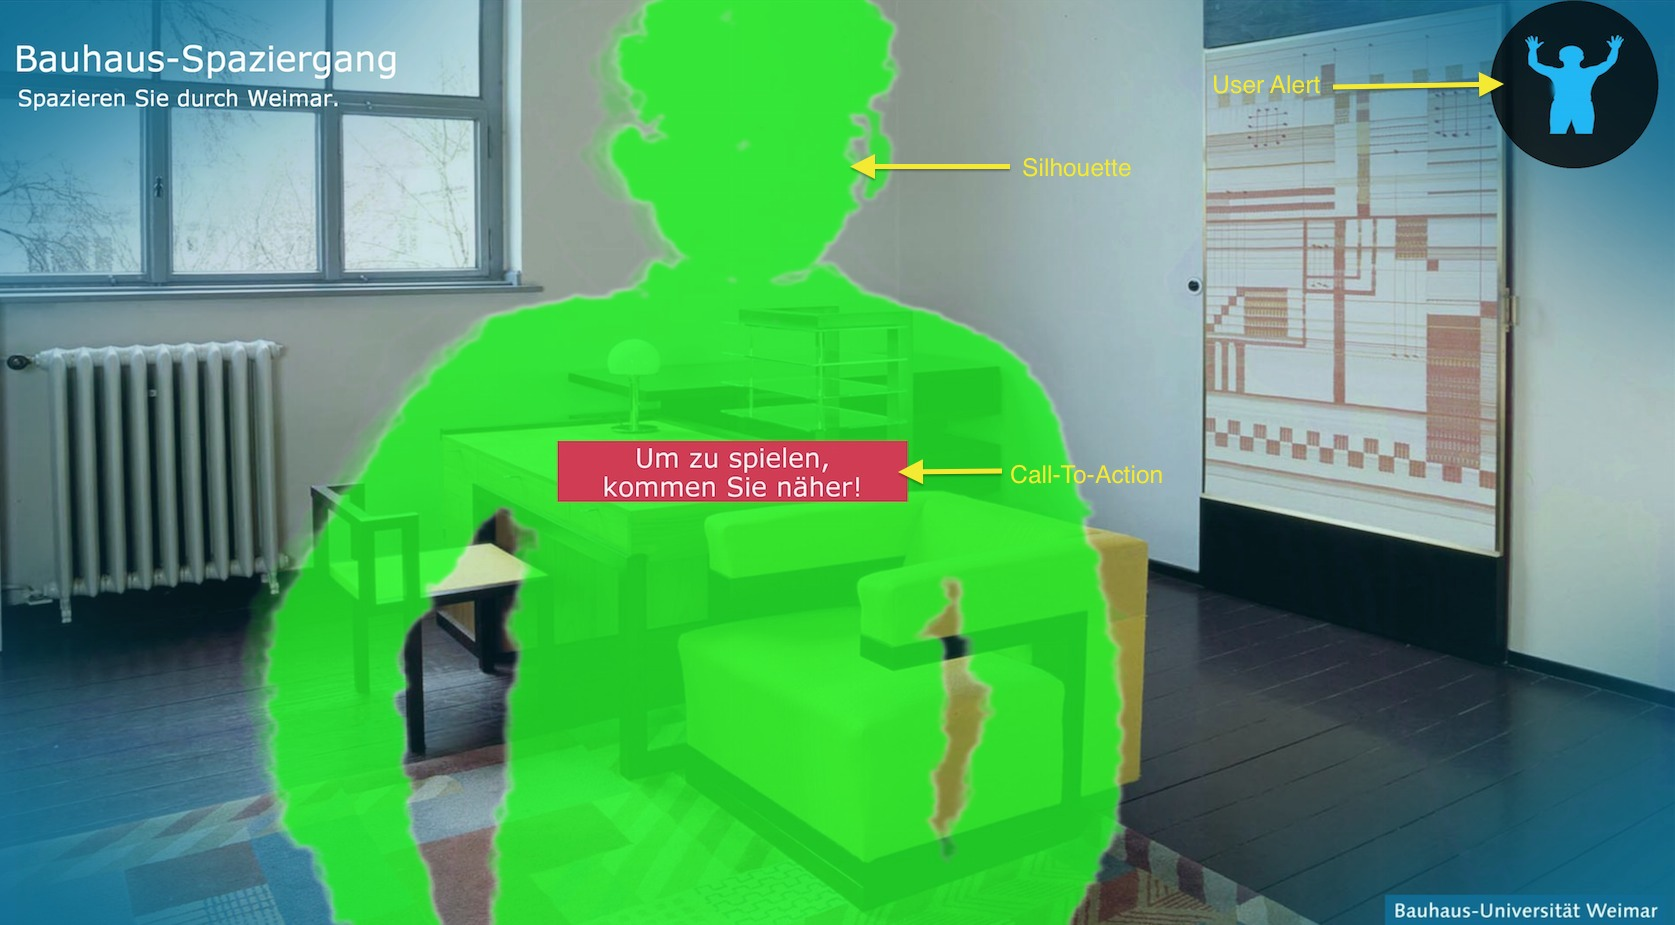
\includegraphics[width=0.8\textwidth,height=70mm]{Figures/7/body_interactive/first_interface}
    \caption{Initial interface}%
    \label{fig:body_firstinterface}%
\end{figure}


\item Transition to Map Interfaces: \\
The transition happens when the person stands close to the screen for more than 3 seconds and the processes is as follow.

\begin{enumerate}
\item Loading animation:\\
 The loading animation is a reaction to the action of the participants, which gives the user a clue that the interaction will be started. 
\item Scaling down the silhouette: \\
To walk freely on the map environment and to give the participant the feeling of real walking. The participant's silhouette is scaled down, the scaling happens smoothly frame-by-frame.
\item Show task instruction:  \\
Every interaction has instructions, the instruction is fairly very easy and it is simplified in one sentence to explore locations on the map.
\end{enumerate}

\begin{figure}[H]
    \centering
    \begin{subfigure}[H]{0.32\textwidth}
        \centering
        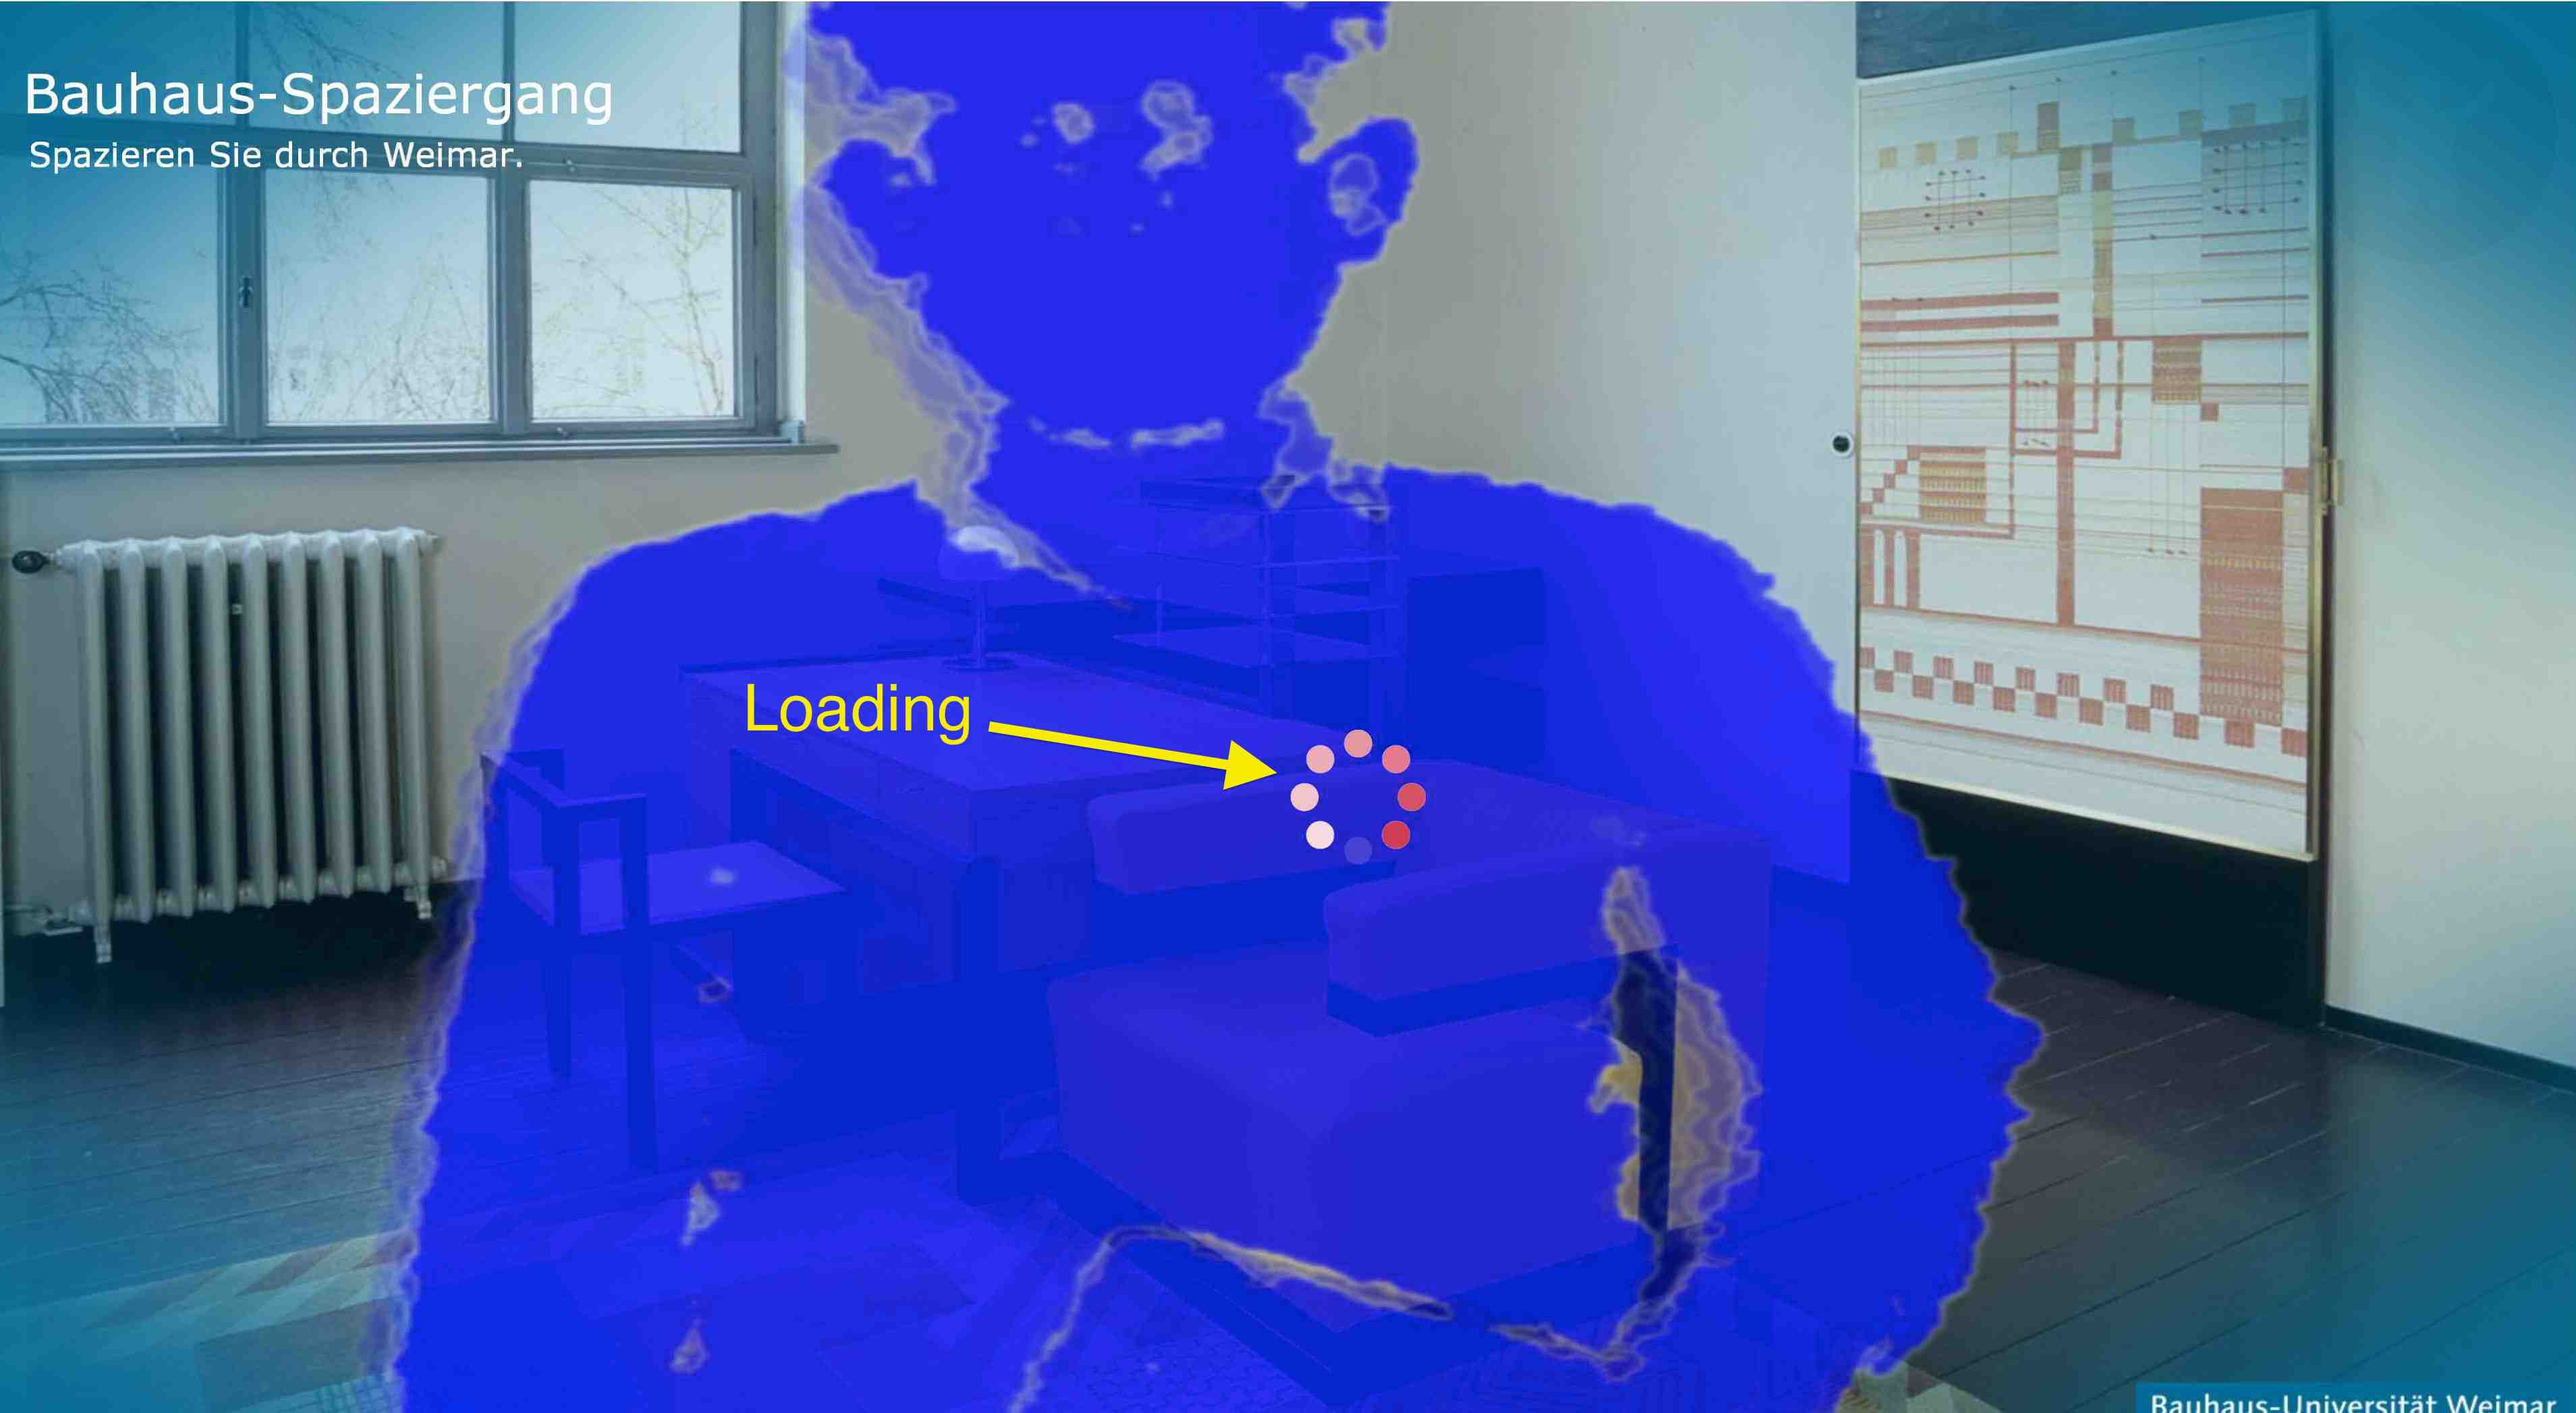
\includegraphics[width=\textwidth,height = 3.5cm]{Figures/7/body_interactive/loading}
        \caption{}
        \label{fig:loading_logo}
    \end{subfigure}
    \begin{subfigure}[H]{0.32\textwidth}
        \centering
        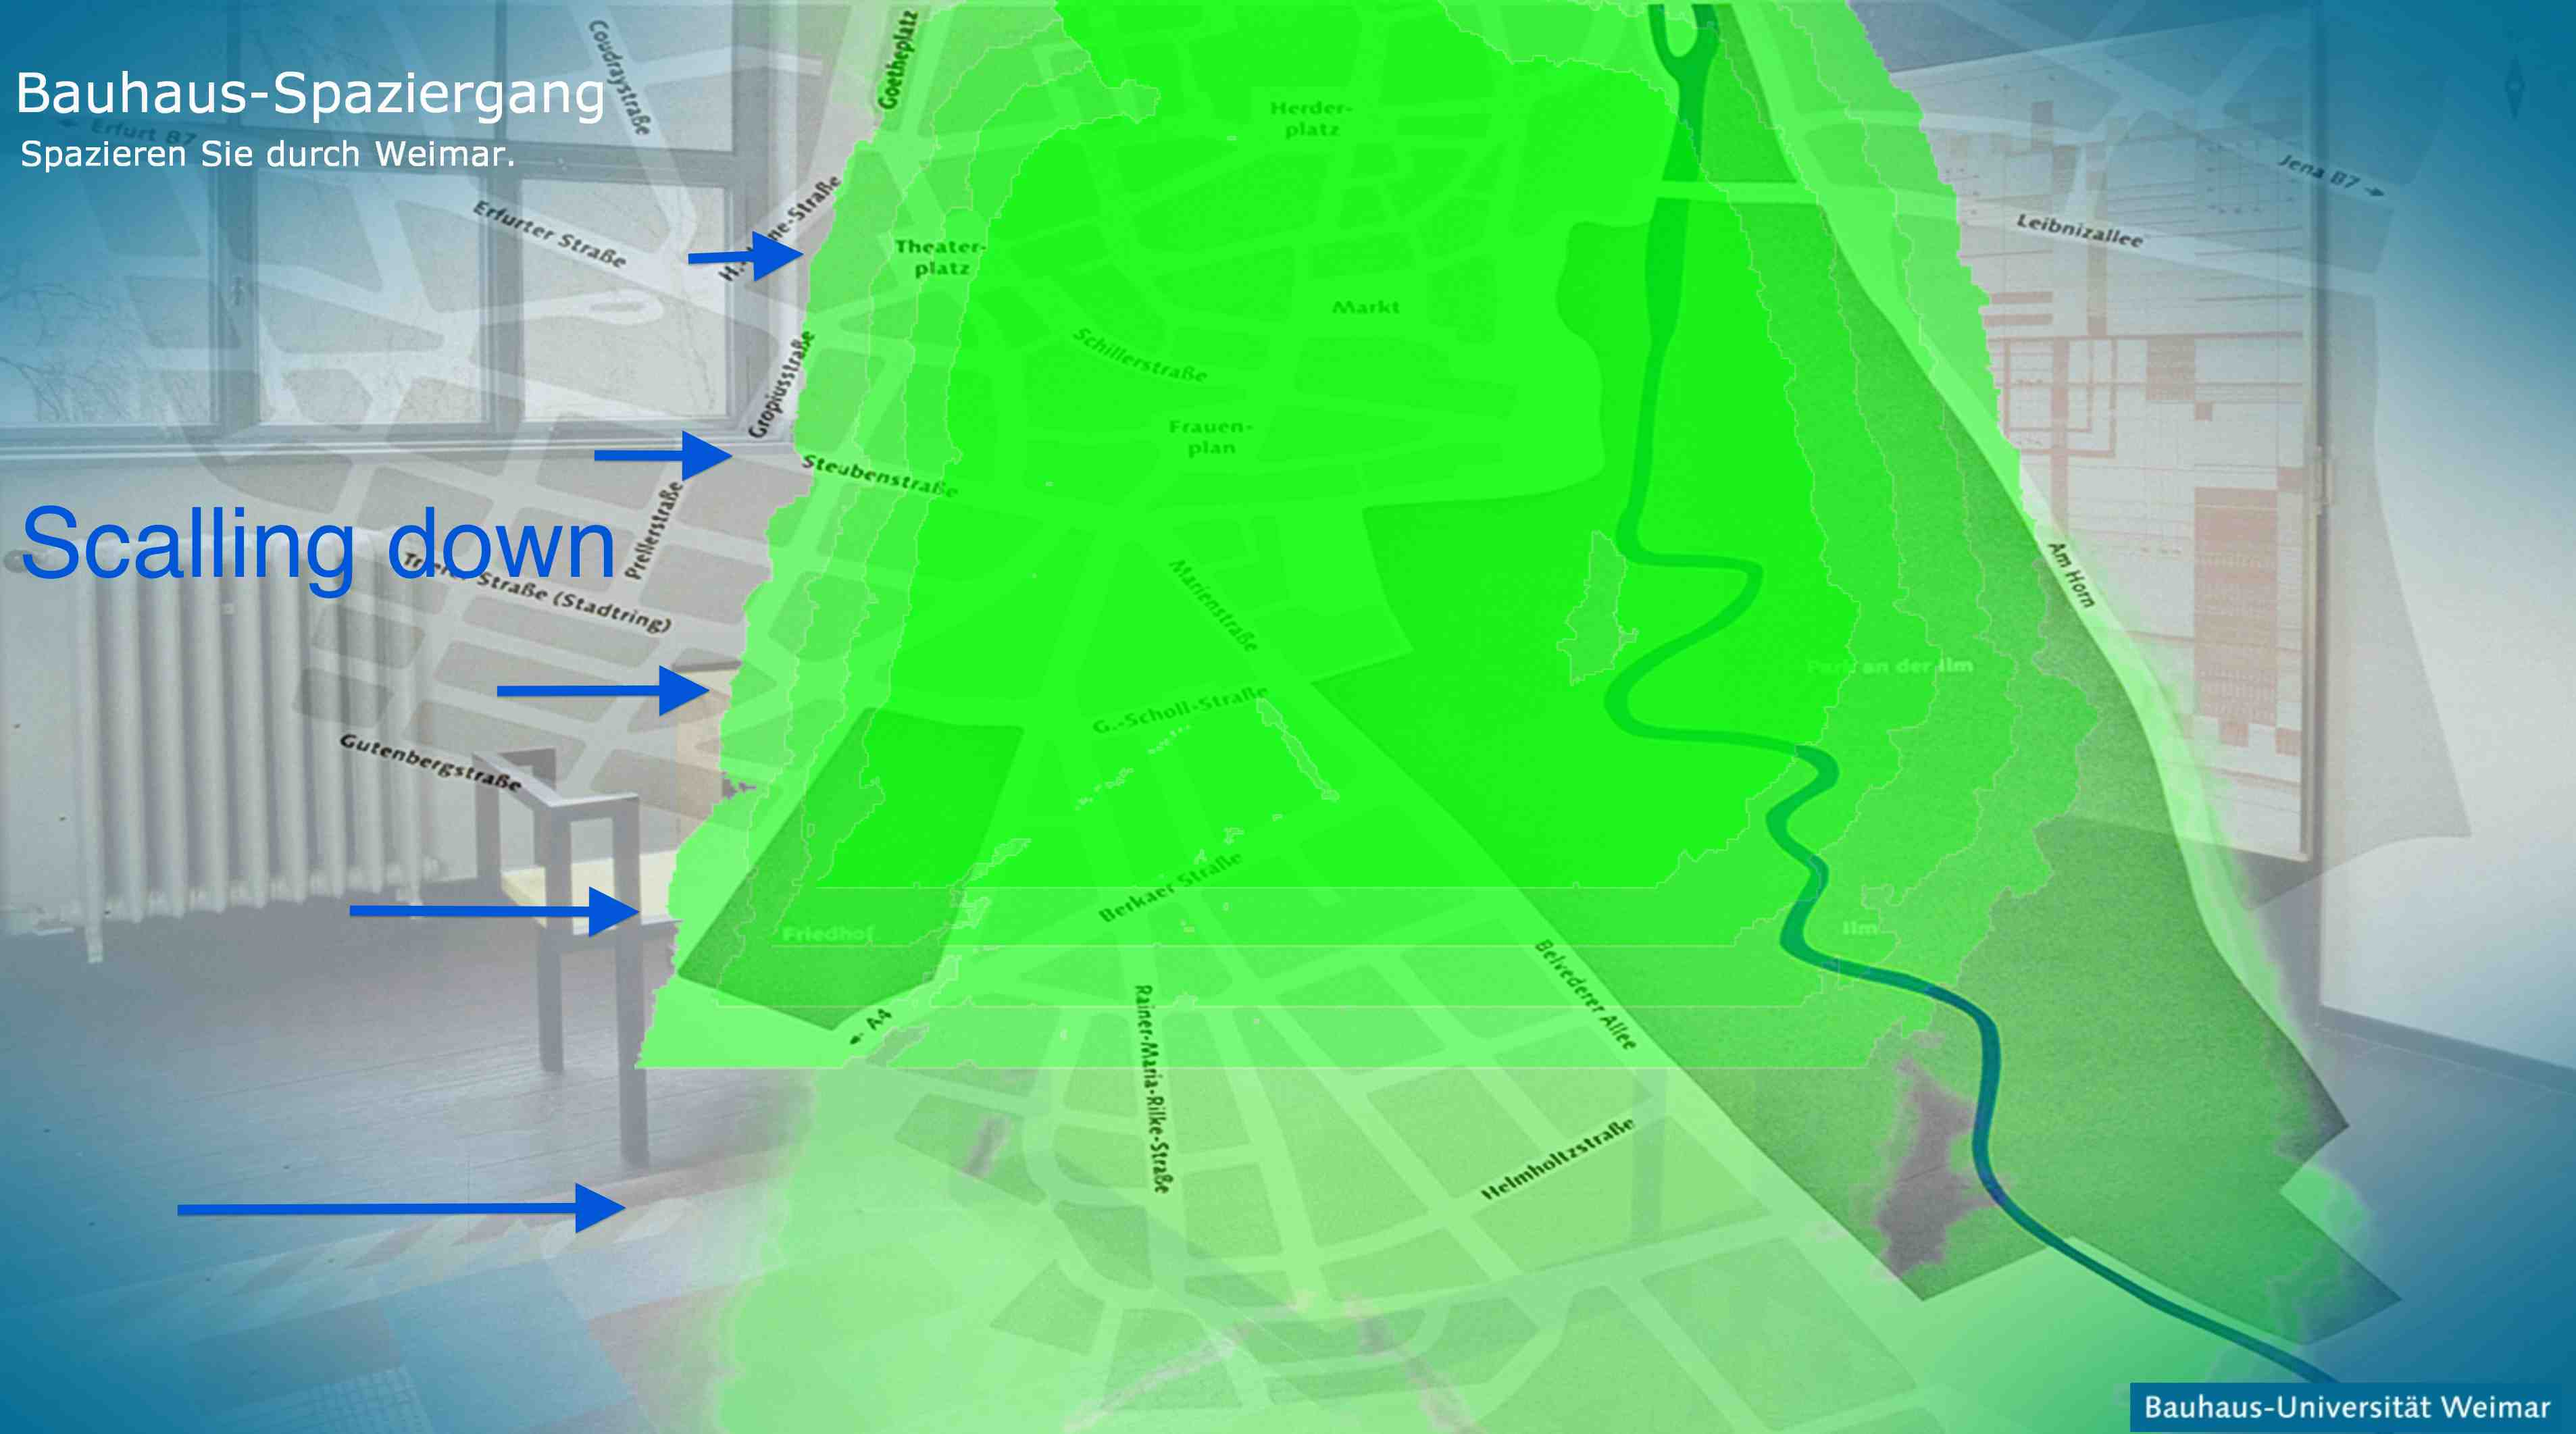
\includegraphics[width=\textwidth,height = 3.5cm]{Figures/7/body_interactive/scalling_down}
        \caption{}
        \label{fig:scalling_down}
    \end{subfigure} 
      \begin{subfigure}[H]{0.32\textwidth}
        \centering
        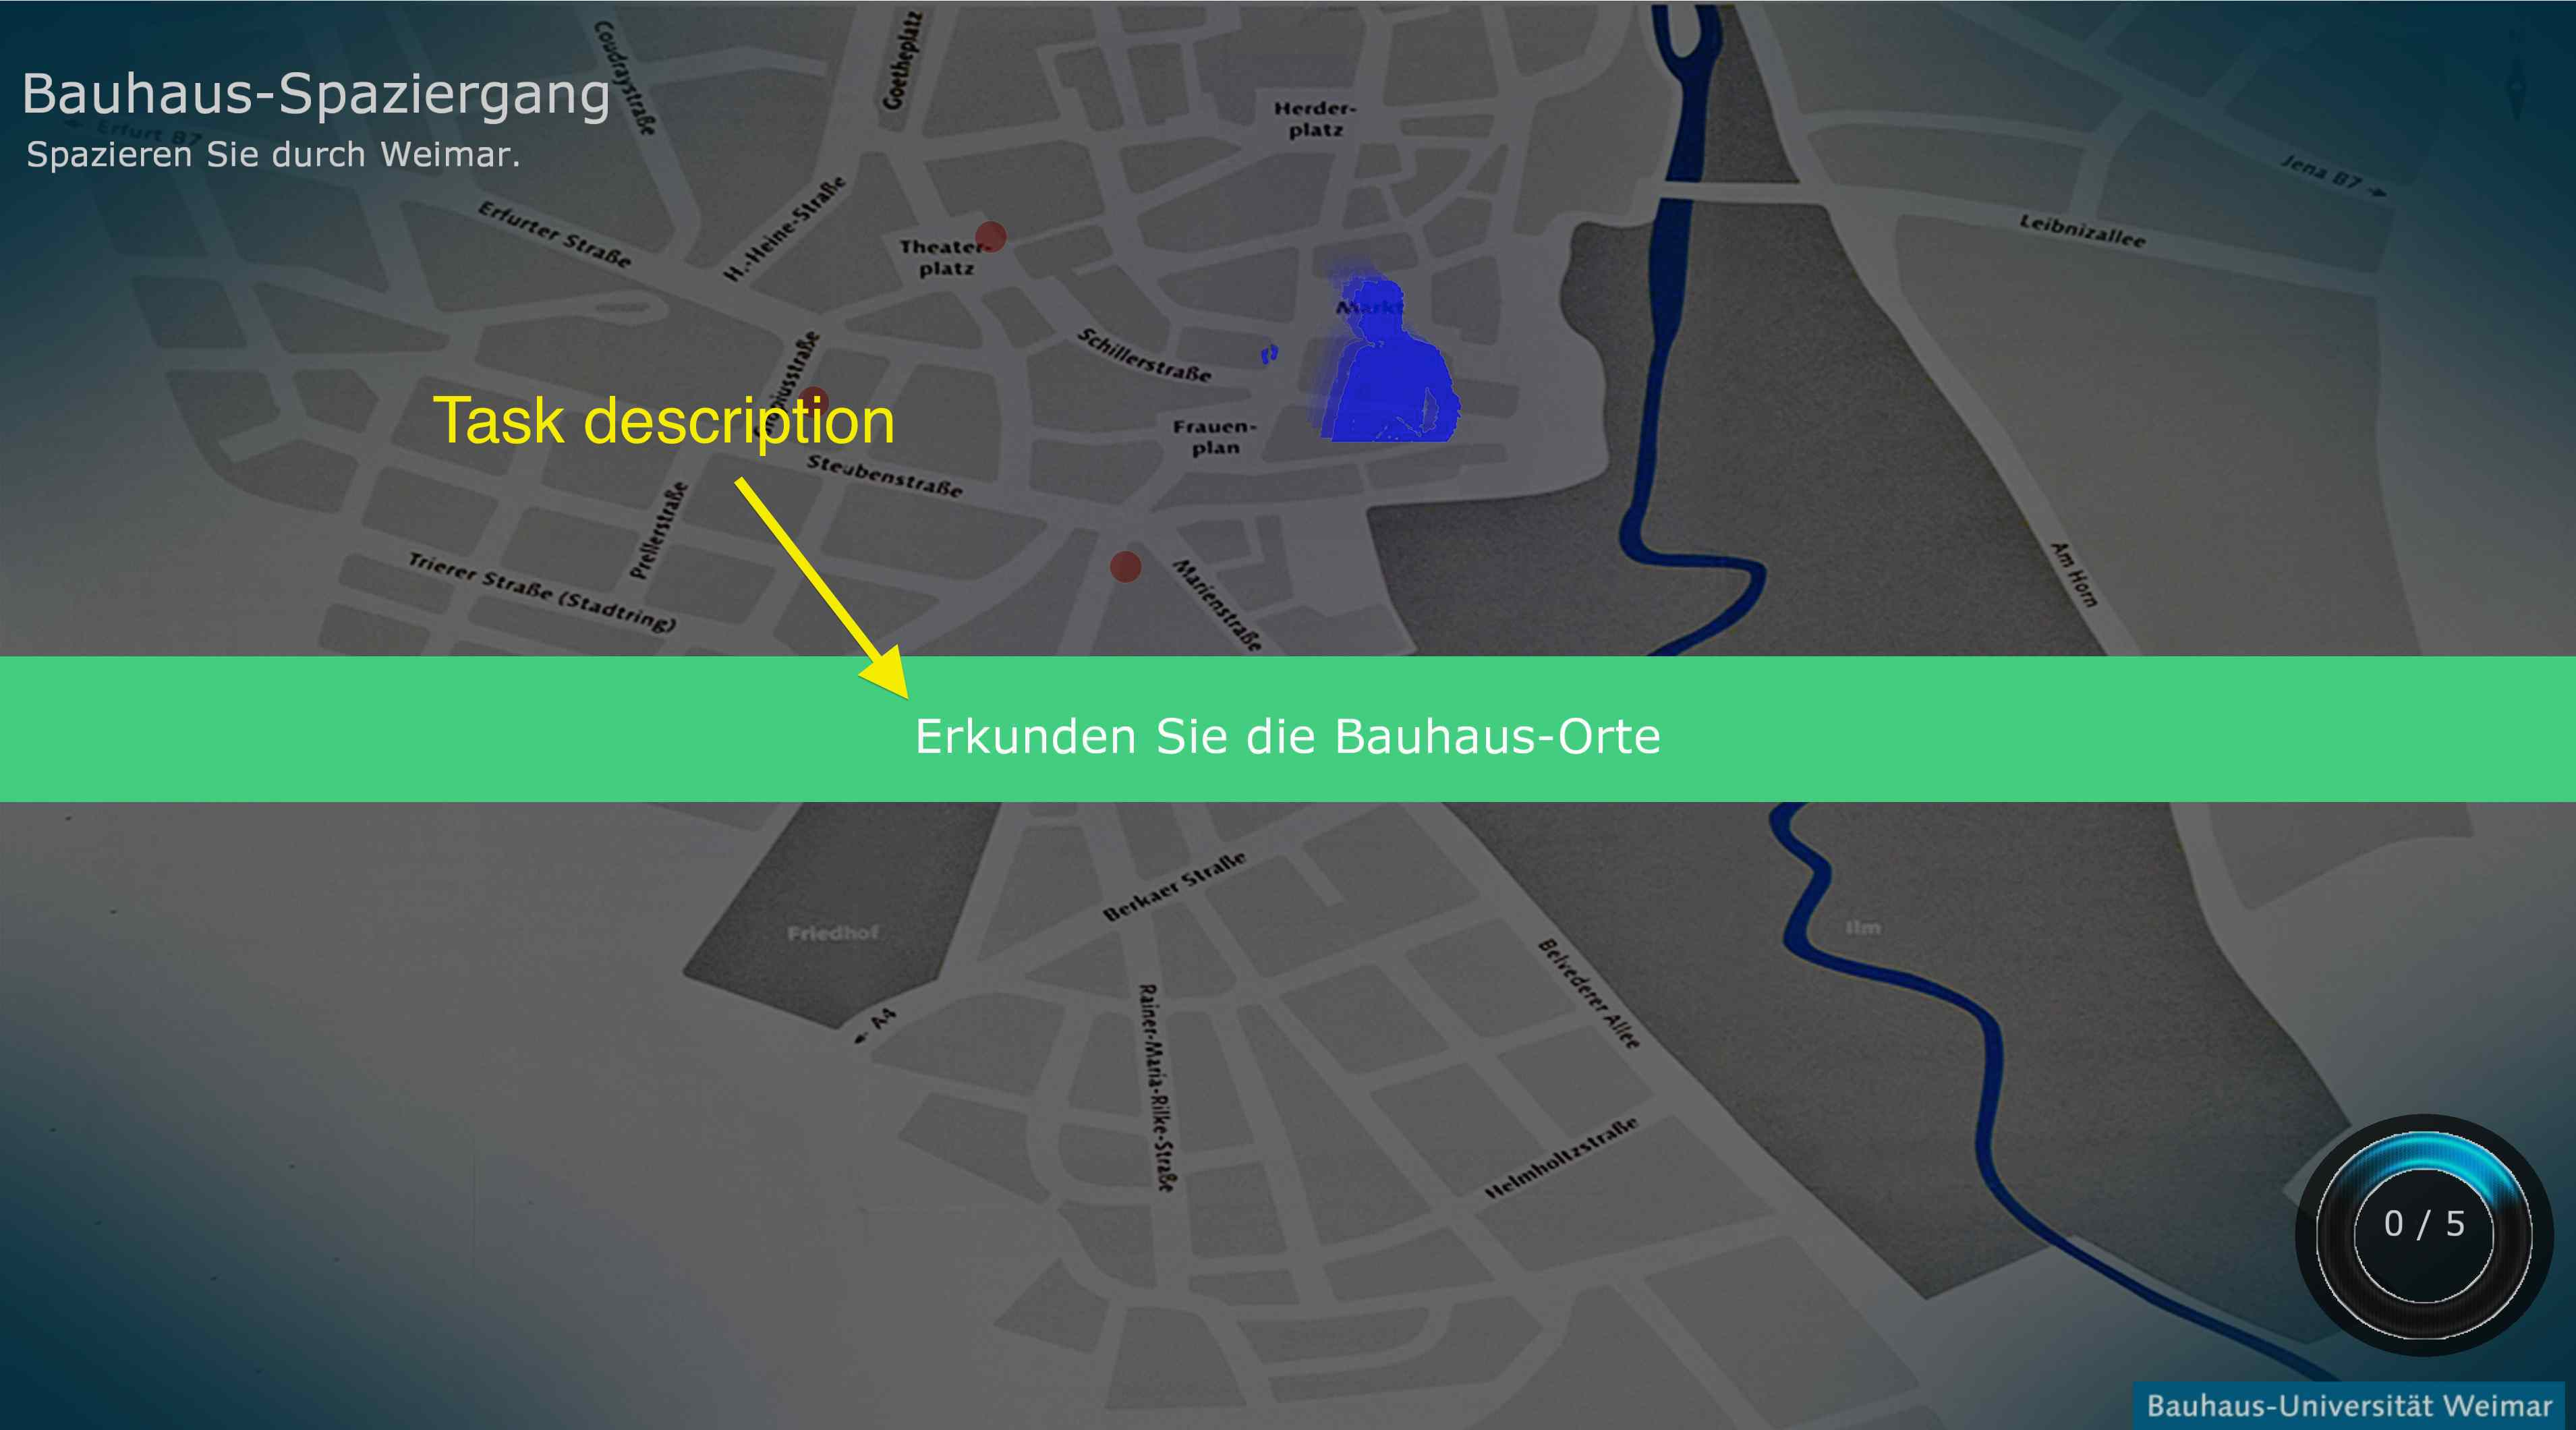
\includegraphics[width=\textwidth,height = 3.5cm]{Figures/7/body_interactive/task_description}
        \caption{}
        \label{fig:task_description}
    \end{subfigure}
    \caption{}
    \label{fig:transition_sequence}
\end{figure}

The picture A shows that the person is close to the screen and the loading of the animation begins. In picture B, the person's silhouette is being scaled down (in this example the silhouette color is green) and in picture C, the instructions are shown.


\item Map Interface (Interaction): \\
In this interface participants can interact with the elements on the map. In the below picture, the silhouette has visited two locations therefore has 2/5 score, to finish the interaction he needs to visit all the location or the timer(40 seconds) on the corner right will be over.\begin{figure}[H]
    \centering
    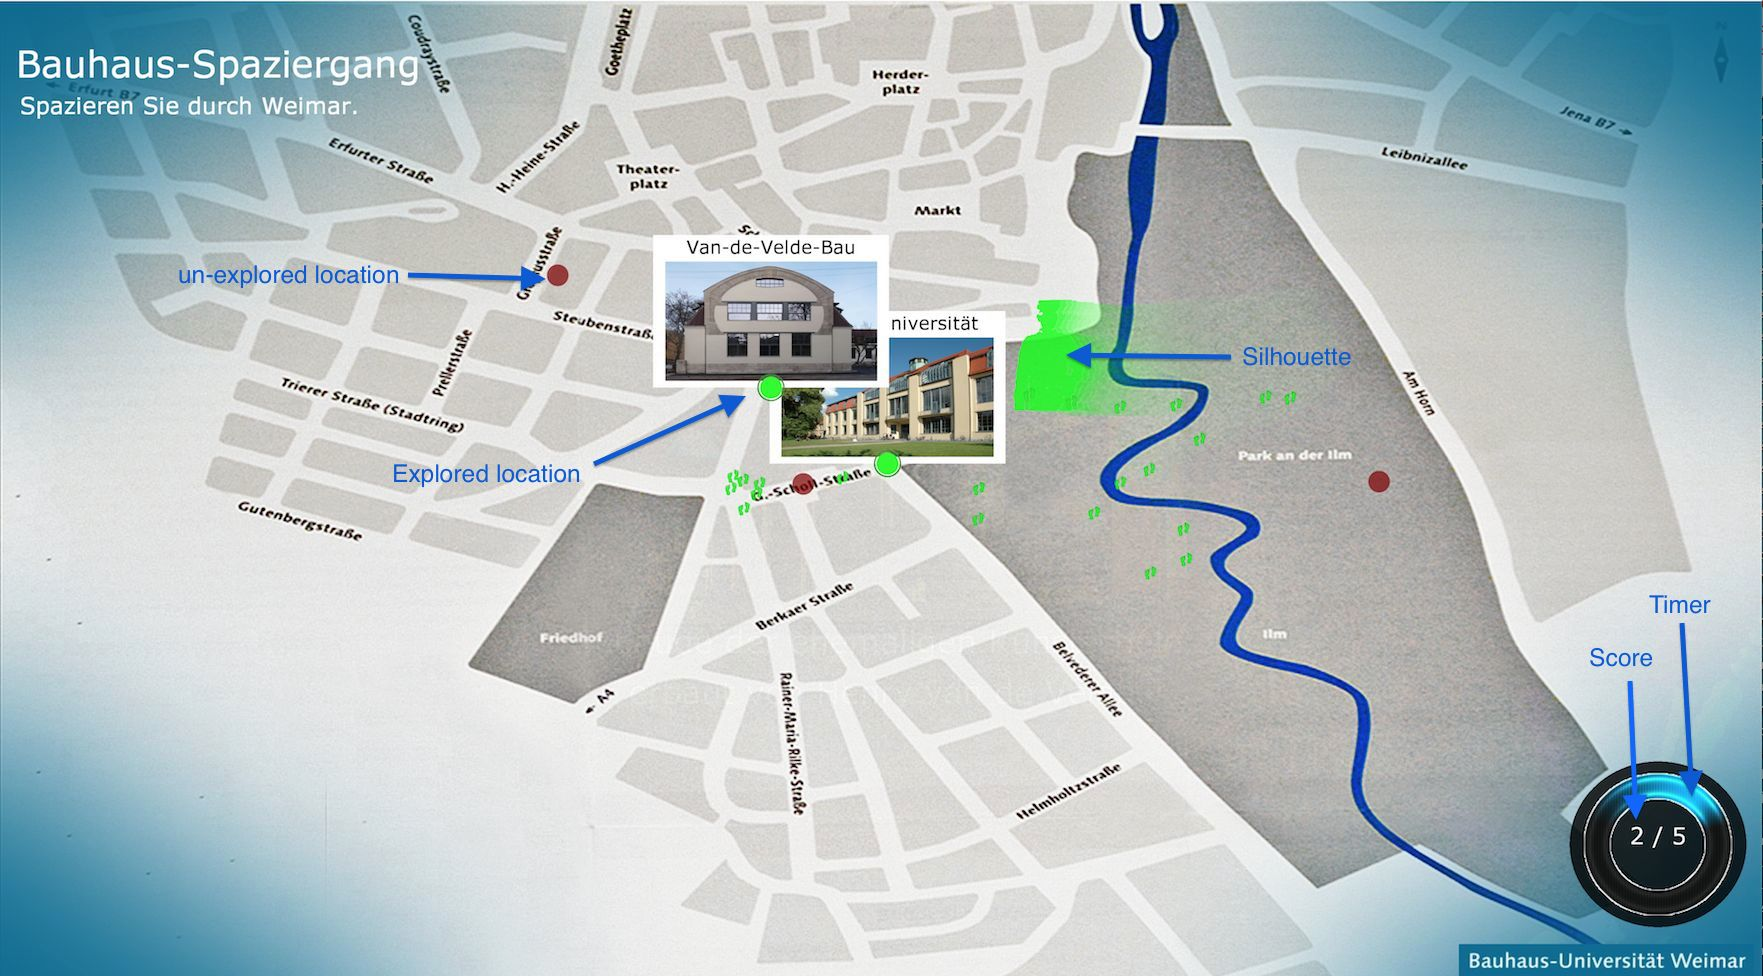
\includegraphics[width=0.8\textwidth,height=70mm]{Figures/7/body_interactive/second_interface}
    \caption{Map Interface}%
    \label{fig:body_secondinterface}%
\end{figure}

\item Advertisement video:\\
The same advertisement video, which was for non-interactive, is shown after the interaction is completed.

\end{enumerate}

\iffalse
\subsubsection{Flowchart Diagram}
The below chart roughly shows the flow of the application.
\begin{figure}[H]
    \centering
    \includegraphics[width=120mm,height=140mm]{Figures/7/body_interactive/body_flow_chart}
    \caption{Body Interactive advertisement Flowchart diagram}%
    \label{fig:Body_flowchat}%
\end{figure}


\subsubsection{Software Details}
The application is developed in Processing language with the support of Kinect Library, The application can run in Windows and OSX operating systems the system should have below requirements.

\begin{itemize}
\item Processing v2.2.2.
\item SimpleOpenNI library for Processing \cite{simpleopenni}
\item 32bit JRE (Java Runtime Environment) v1.8 or higher.
\item Windows / Mac OSX
\item RAM: 4GB or above.
\item CPU: Core i5 / i7 2.3Ghz
\end{itemize}

Refere to Appendix \ref{app:fileandfolders} to look for paths of the source code in DVD. The DVD has all the libraries and important things you require to run the application.

\fi

\subsection{Mobile Interactive application}
In this application, the display interface is absolutely the same as the other two applications; the only different is that a user carries out the interaction with a smartphone. The mobile interaction technique and platform was adapted from the Bauhaus University \emph{MMM Ball}\cite{MMMball, MMMball2} project under Mobile Media Group\footnote{Mobile Media Group: \url{https://www.uni-weimar.de/de/medien/professuren/mobile-media/}, last accessed 5 jun 2016} department.

\begin{enumerate}

\item Initial Interface (\emph{Call-to-Action}) : \\
This interface is designed in such a way to attract passersby and also guide the participants on how to use their smartphone to access the advertisement application. The attraction is again the same method that was used for the body, the passersby silhouette is projected at the back of Access information. The interface has a QR code that could be easily scanned instead of typing the whole IP address. There is an alert area that gets activated when a logged in person has not turned their phone in landscape orientation.
\begin{figure}[H]
    \centering
    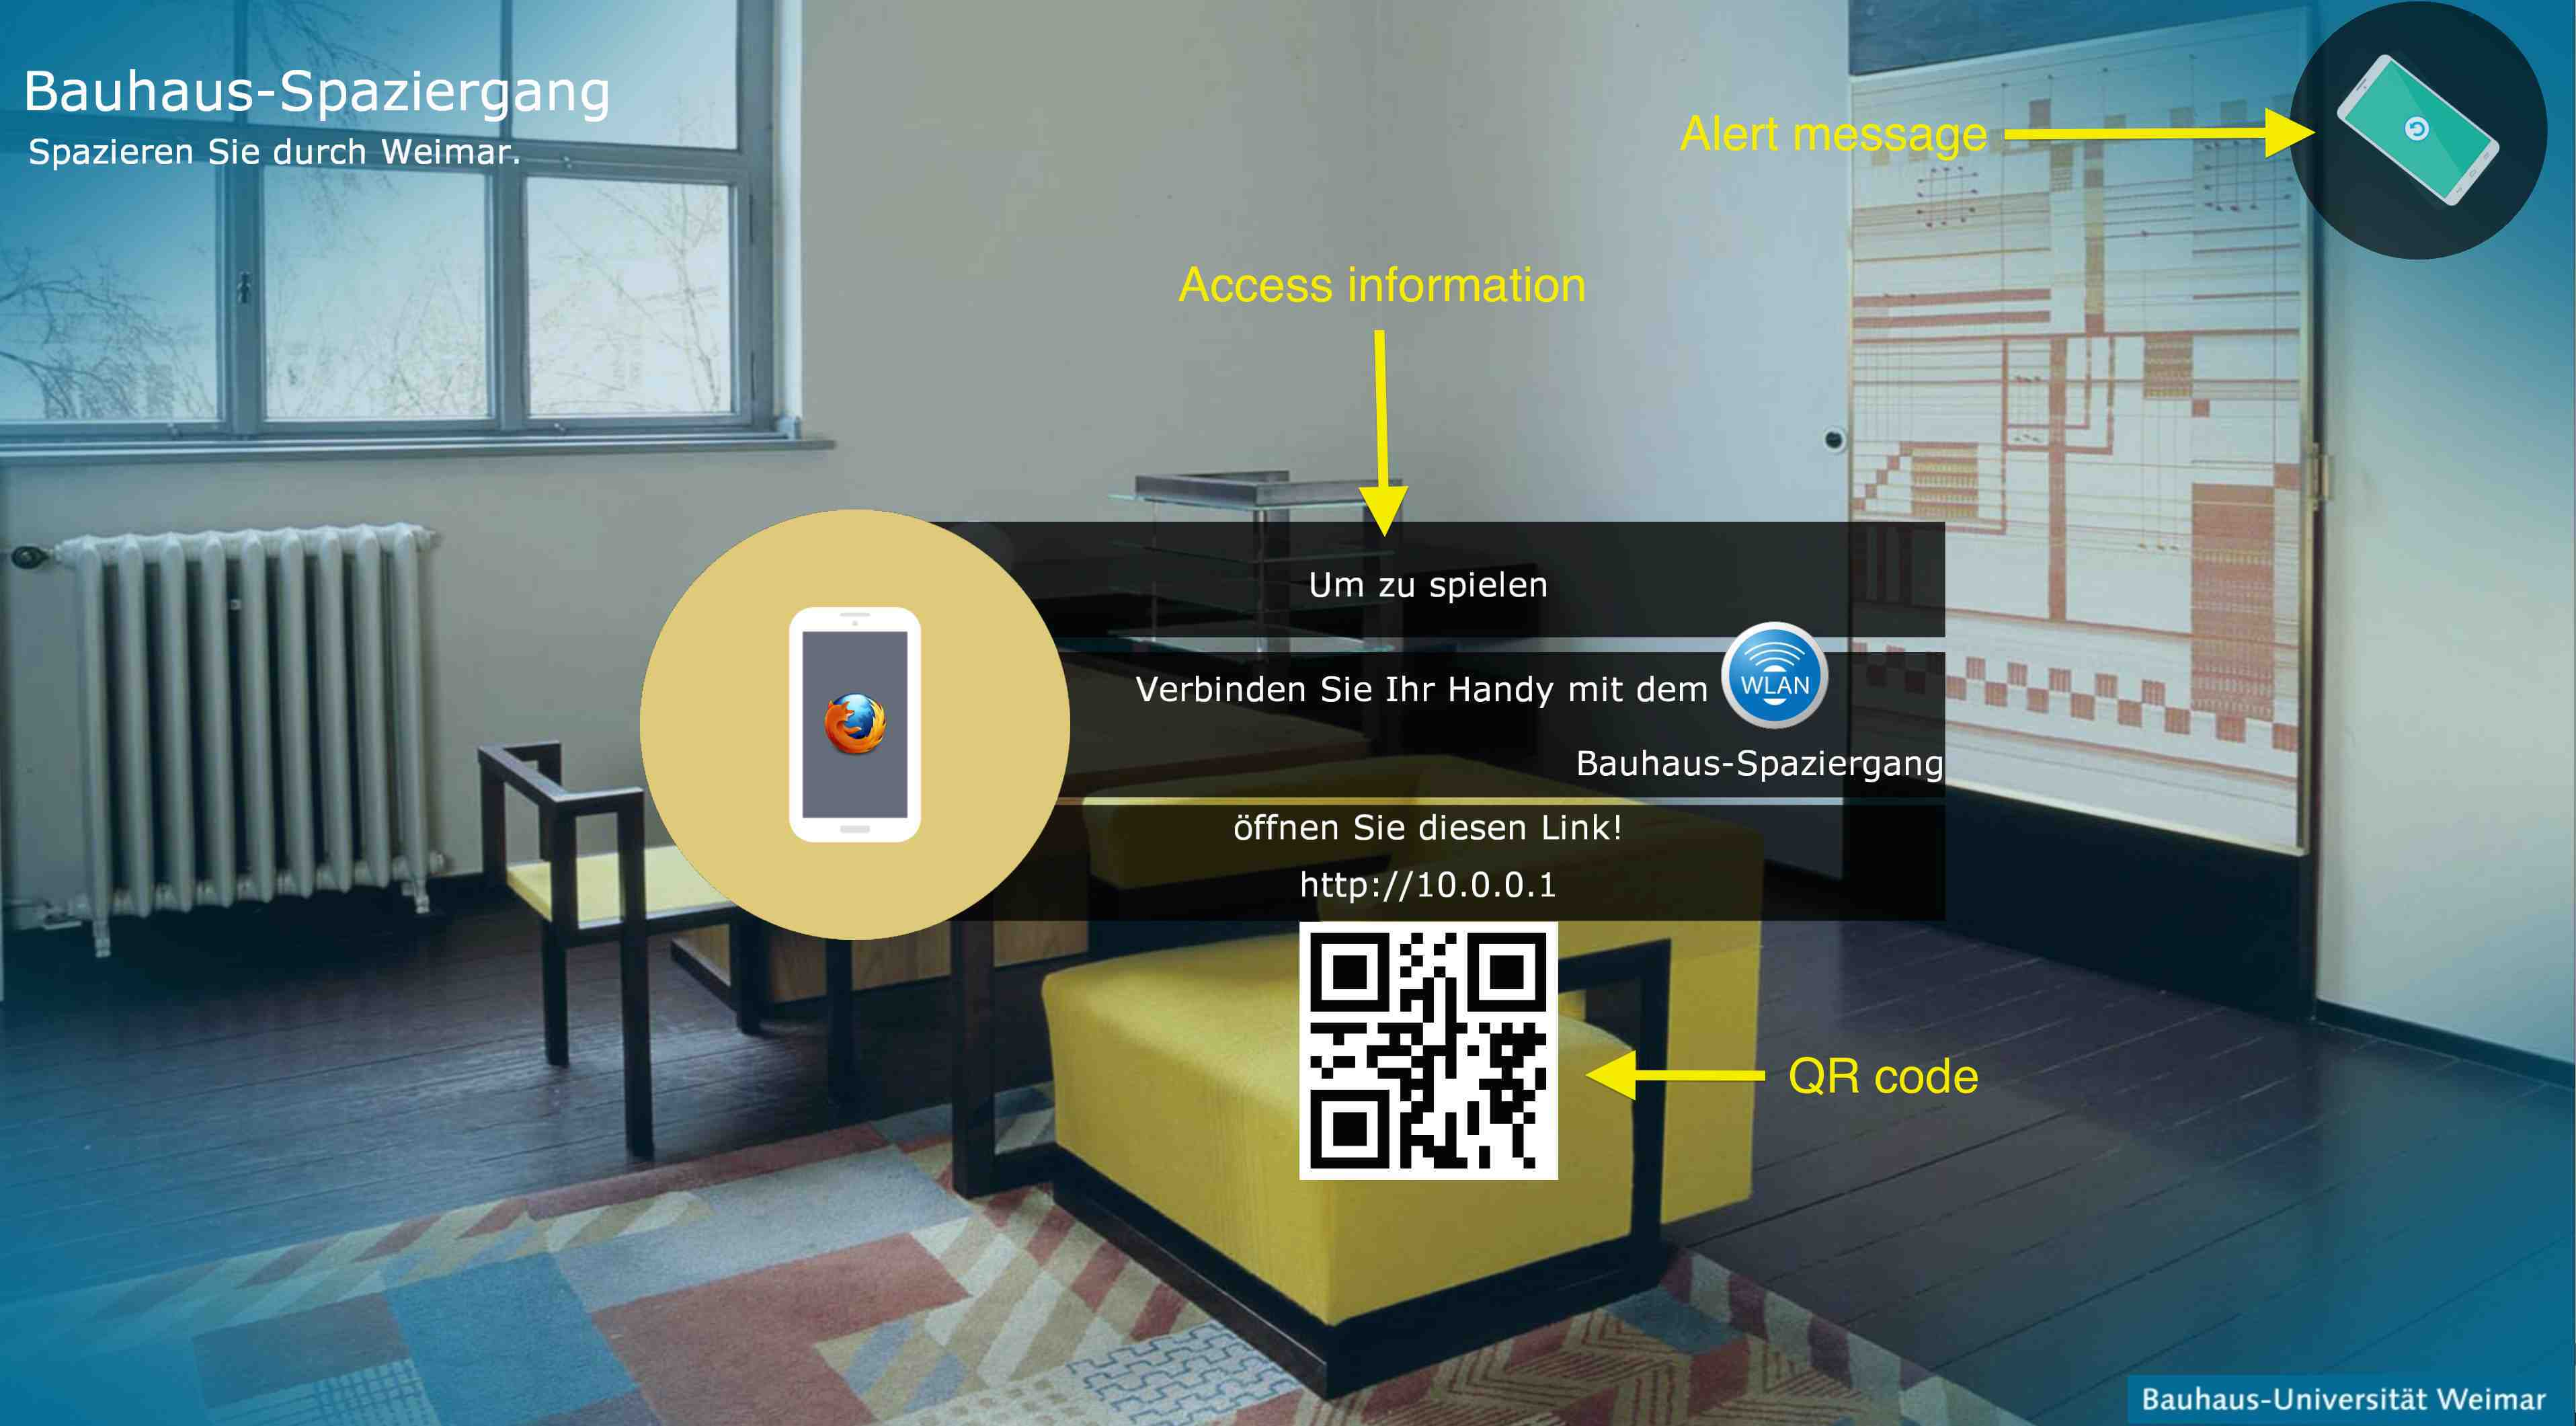
\includegraphics[width=0.8\textwidth,height=70mm]{Figures/7/mobile_interactive/first_interface}
    \caption{Initial Interface}%
    \label{fig:mobile_firstinterface}%
\end{figure}



\item Transition to Map Interface: \\
The user should login to the advertisement system, open the interaction controller, hold the mobile in landscape mode and then the following process will be triggered. 

\begin{enumerate}
\item Loading animation:\\
The loading animation is a reaction to the action of the participants, which gives the user a clue that the interaction will be started. 
\item  Creating Colored cursor: \\
A colored circle will be created for the participant in the center of the screen; each participant would have different colors matching to their controller interface in their phone.
\item Show task instruction:  \\
The instruction is fairly very easy and it is simplified in one sentence to explore locations on the map by using their phone.

\end{enumerate}


\begin{figure}[H]
    \centering
    \begin{subfigure}[H]{0.48\textwidth}
        \centering
        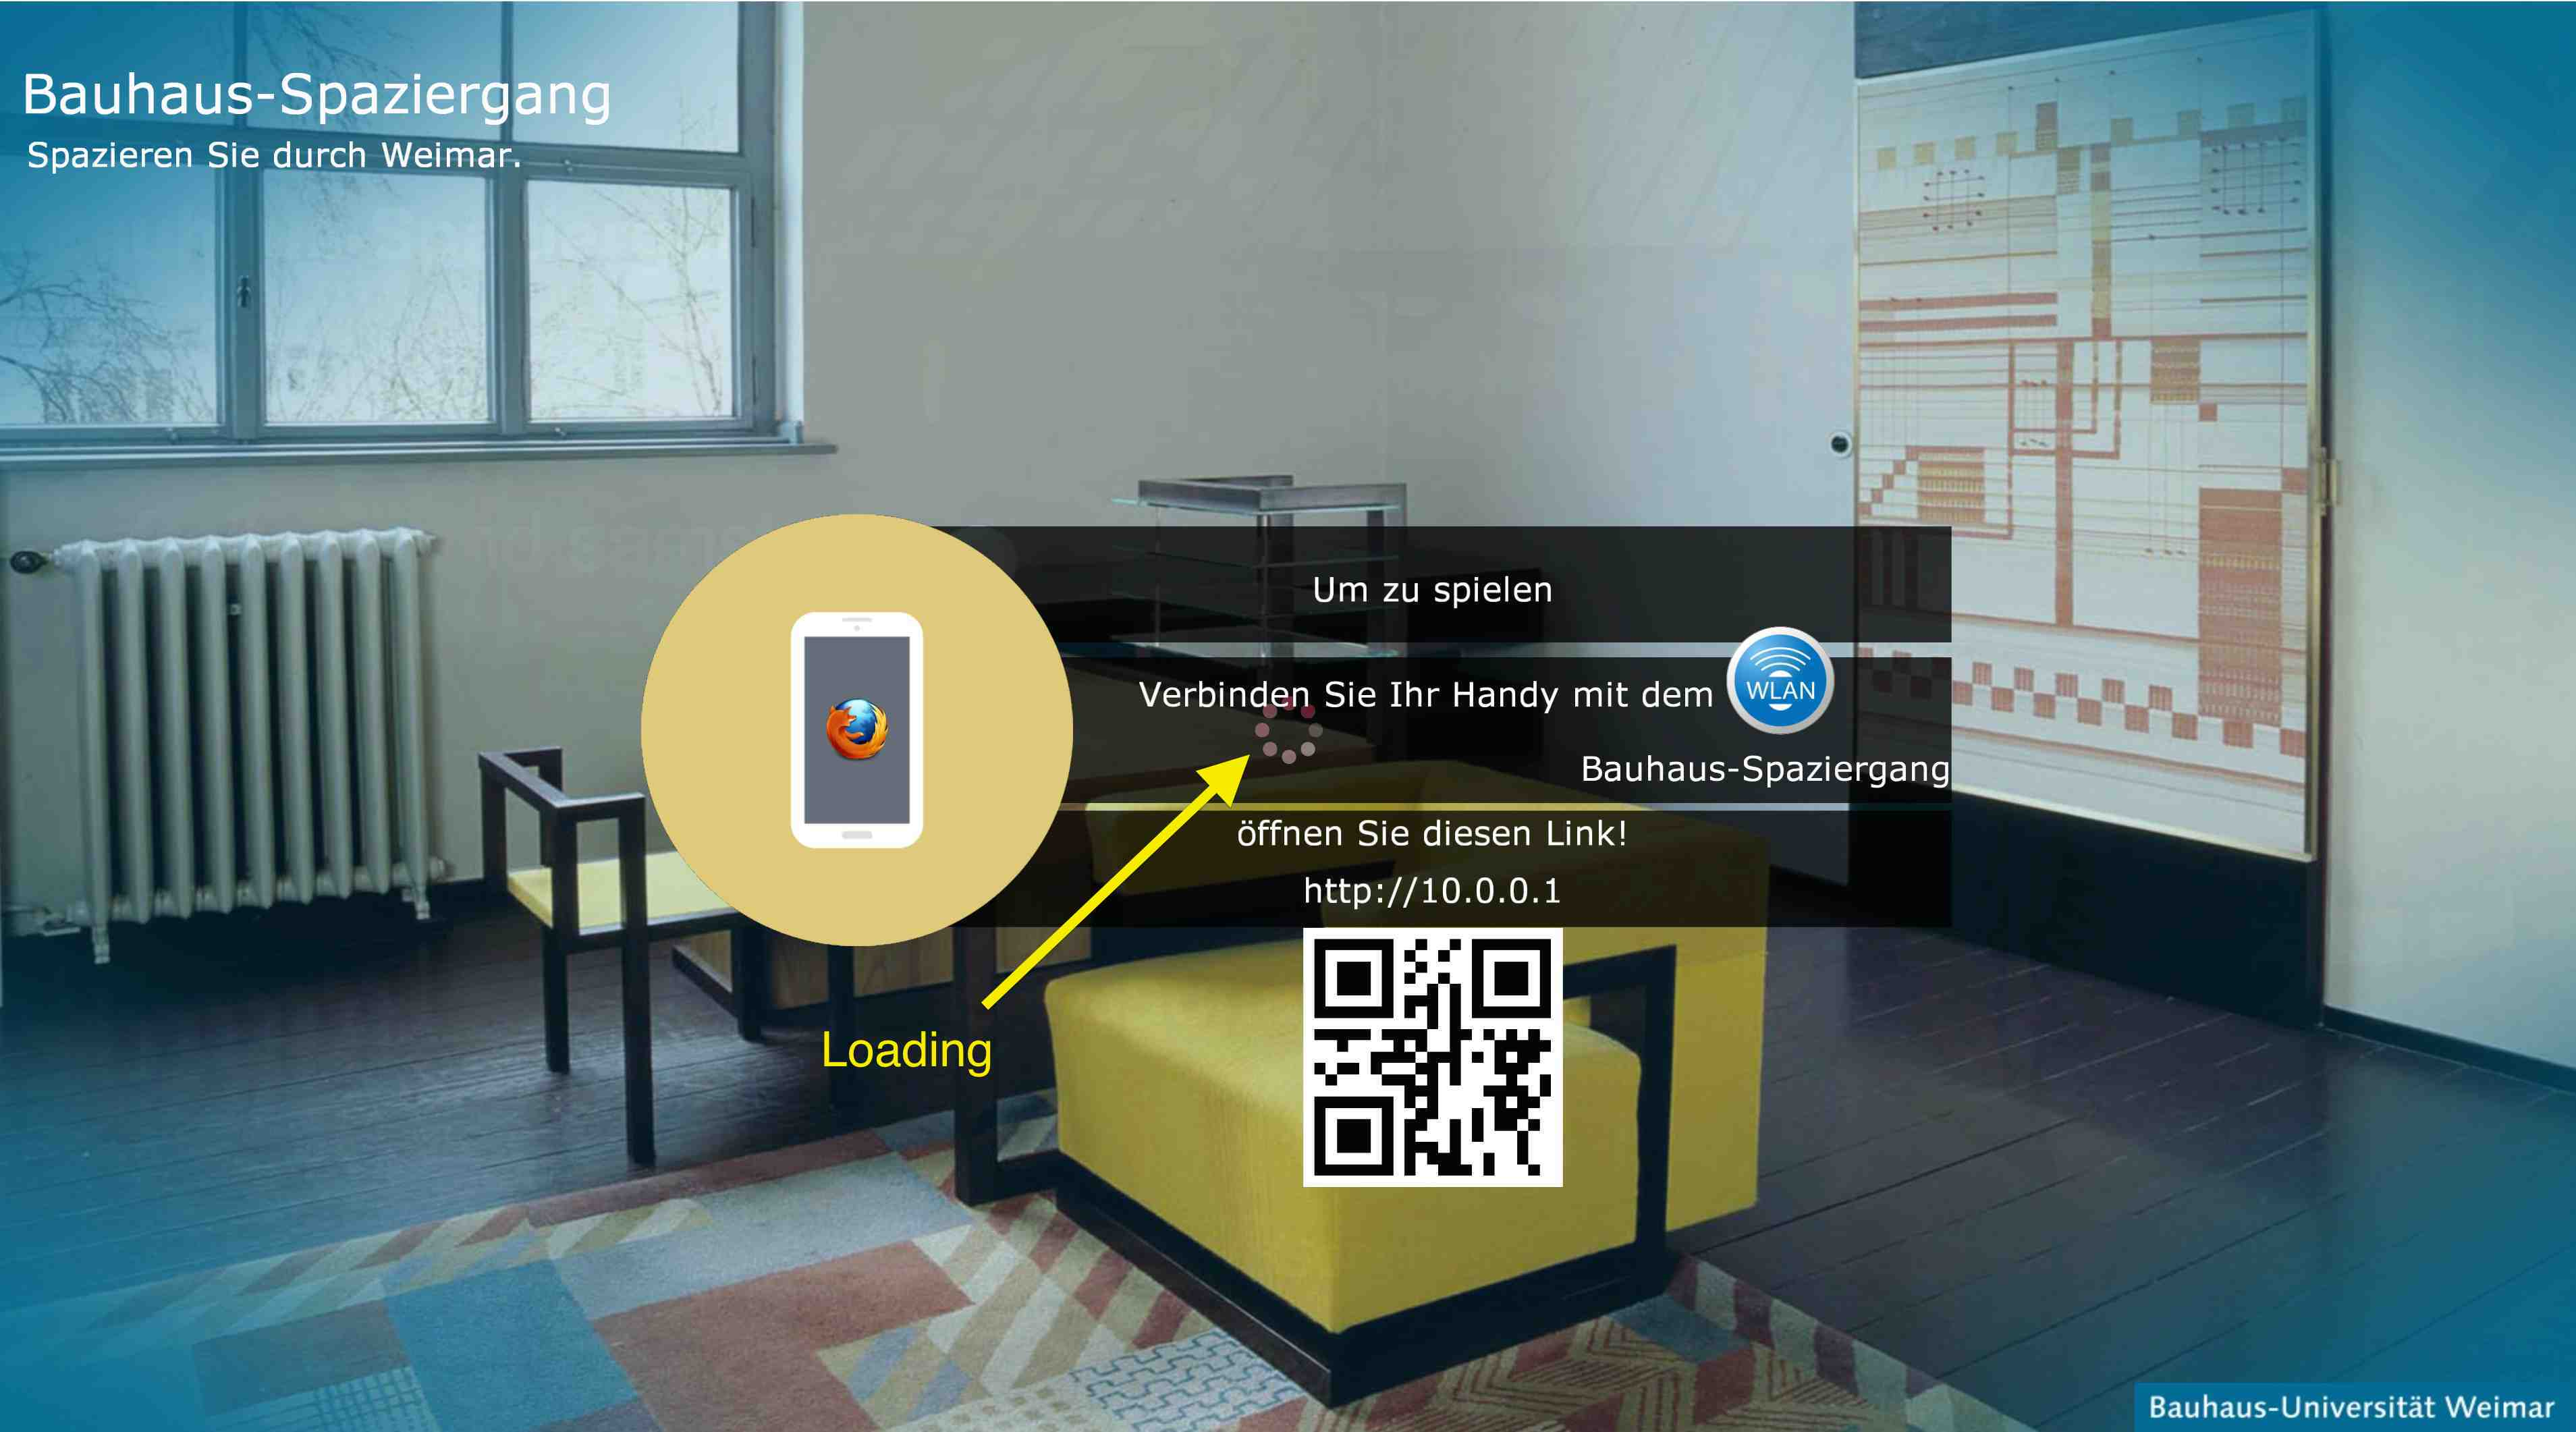
\includegraphics[width=\textwidth,height=5cm]{Figures/7/mobile_interactive/loading}
        \caption{}
        \label{fig:loading_mobile}
    \end{subfigure}
    \begin{subfigure}[H]{0.48\textwidth}
        \centering
        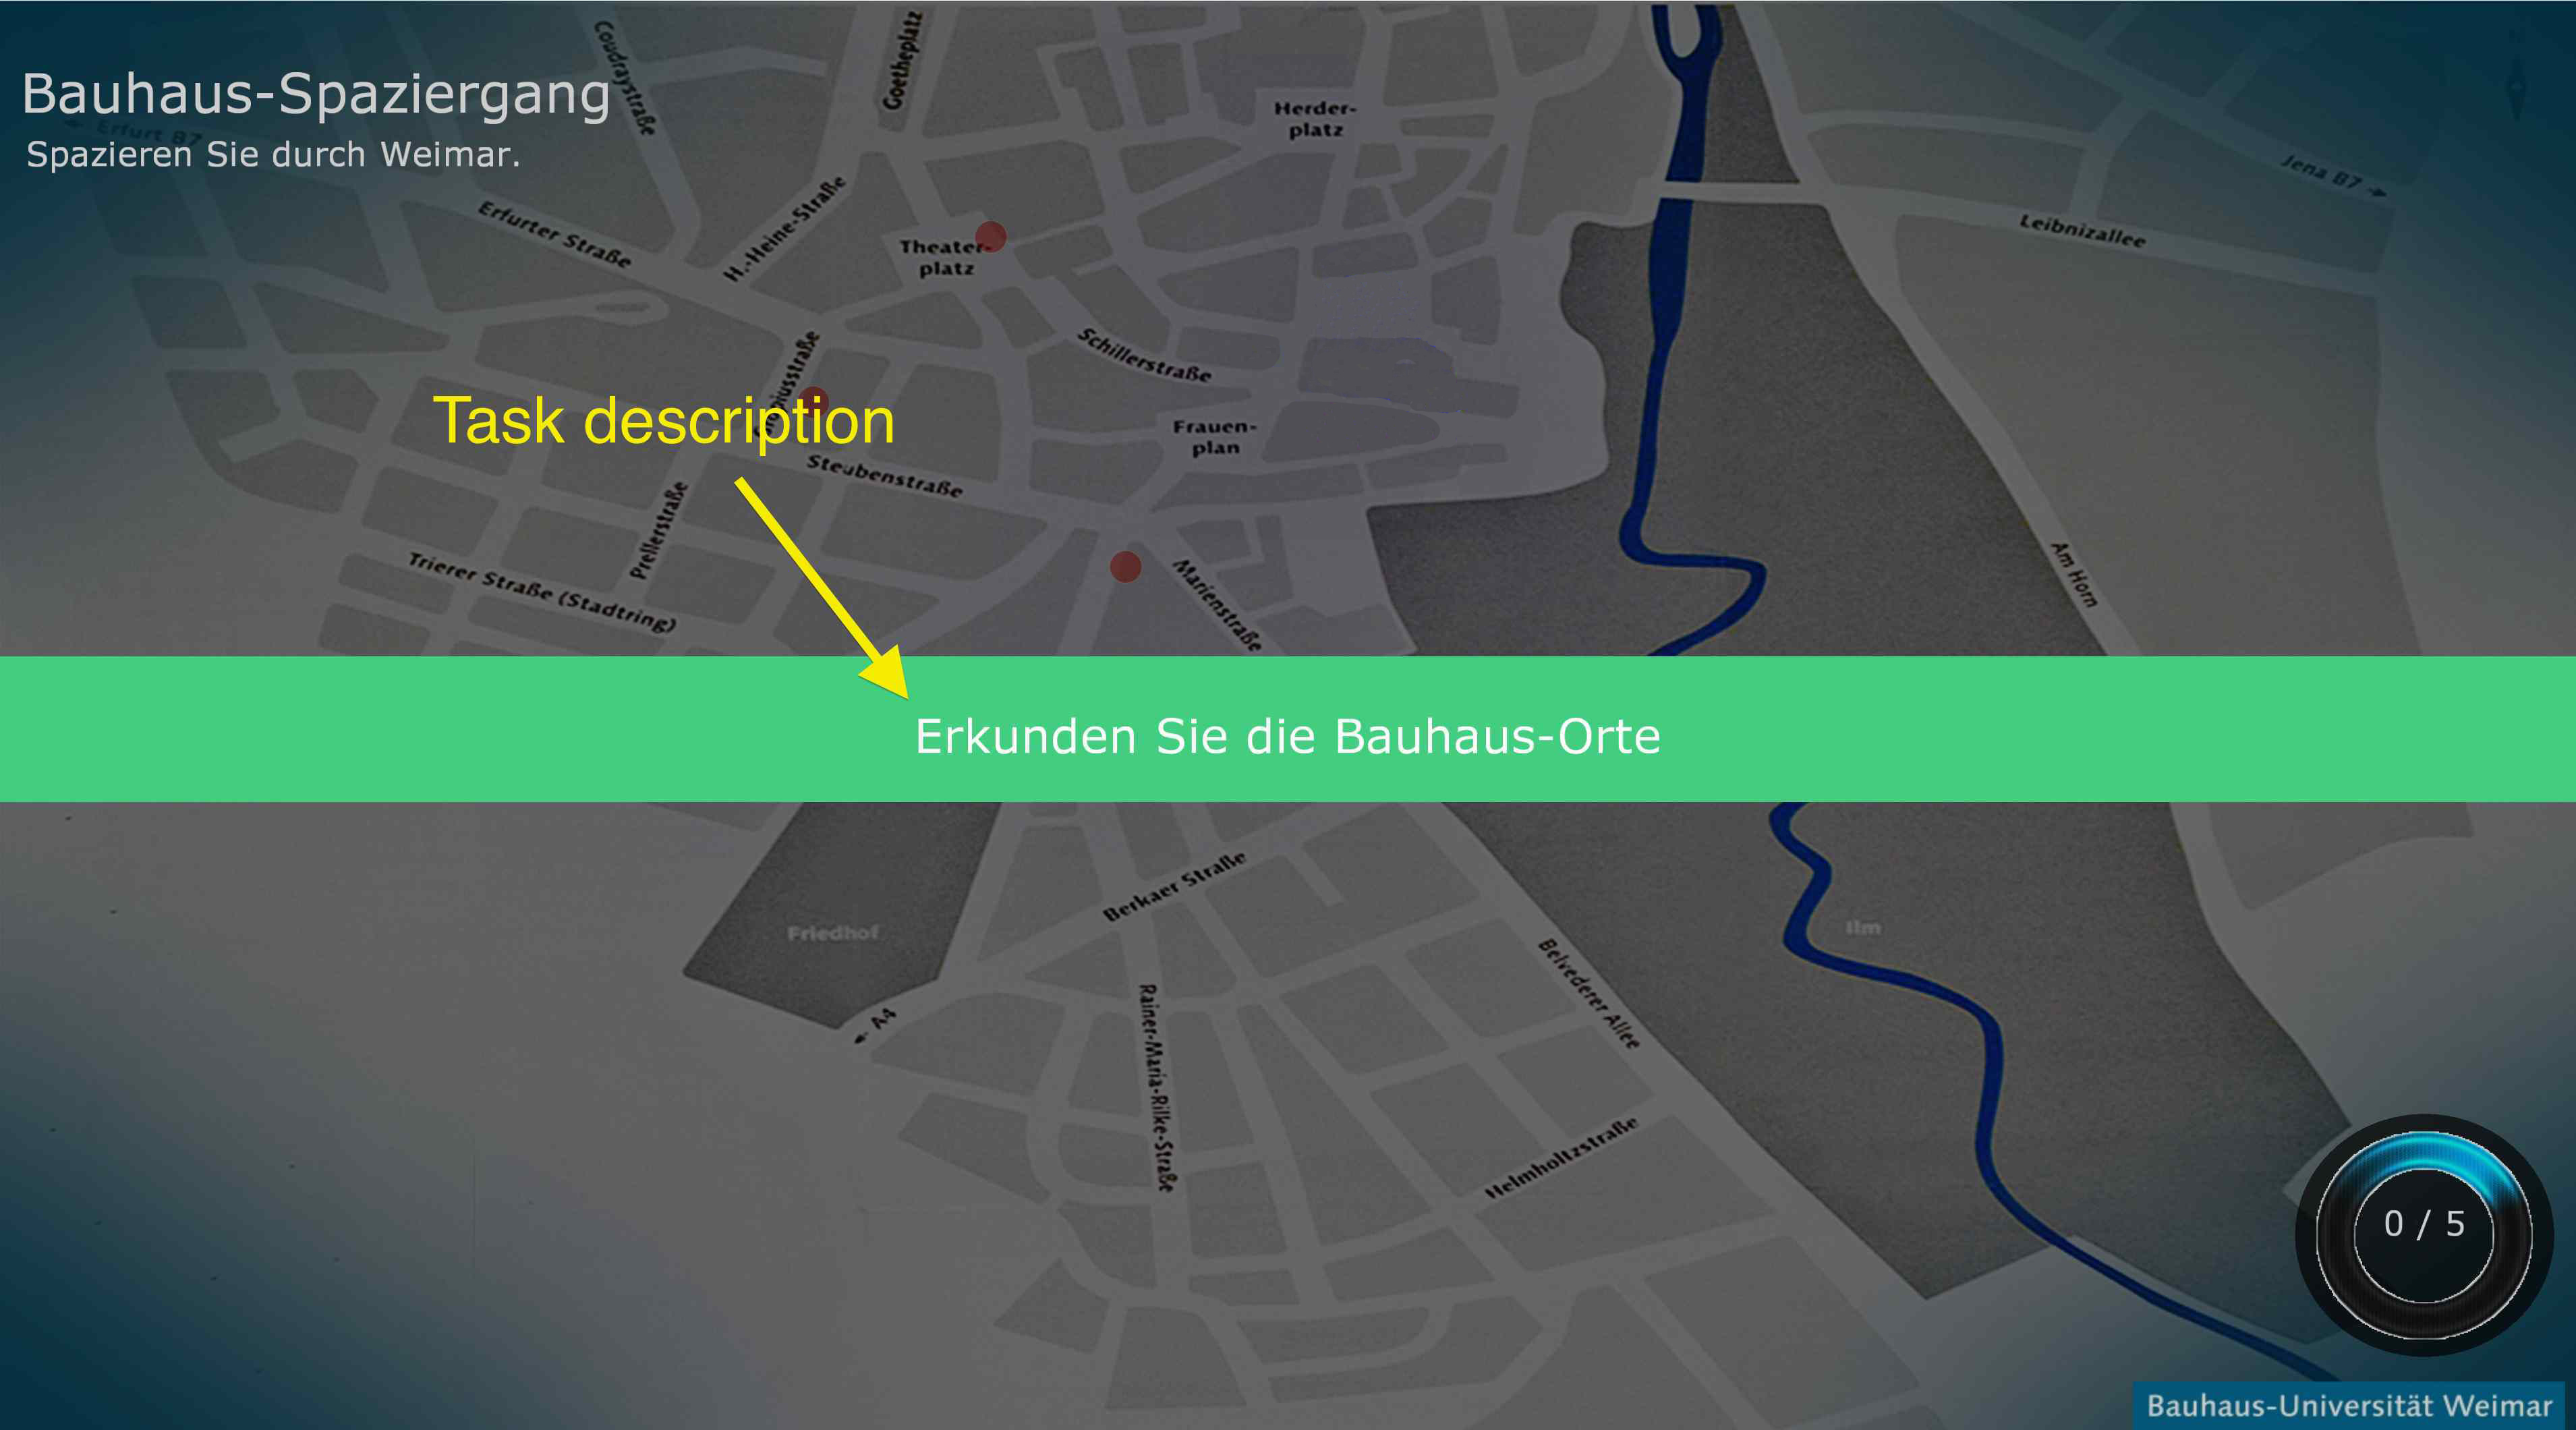
\includegraphics[width=\textwidth,height=5cm]{Figures/7/mobile_interactive/task_description}
        \caption{}
        \label{fig:task_mobile}
    \end{subfigure}
    \caption{Transition of interface}
    \label{fig:Switching_between_phases_mobile}
\end{figure}

In picture (A) a user has logged in and the screen is loading, in picture (B) the task description is shown.


\item Map Interface (Interaction): \\
This interface is where the users interact with the map; participants can navigate using the controller page on their phones. The image \ref{fig:mobile_secondinterface} displays that the user is controlling the cursor and has explored one location. The user's defined login name is also shown on the cursor to provide a hint that he/she is his circle. To reach an interest point a small circle is shown to determine the area of intersection. The interaction finishes when all the locations are explored or the interaction time (40 seconds) gets over.


\begin{figure}[H]
    \centering
    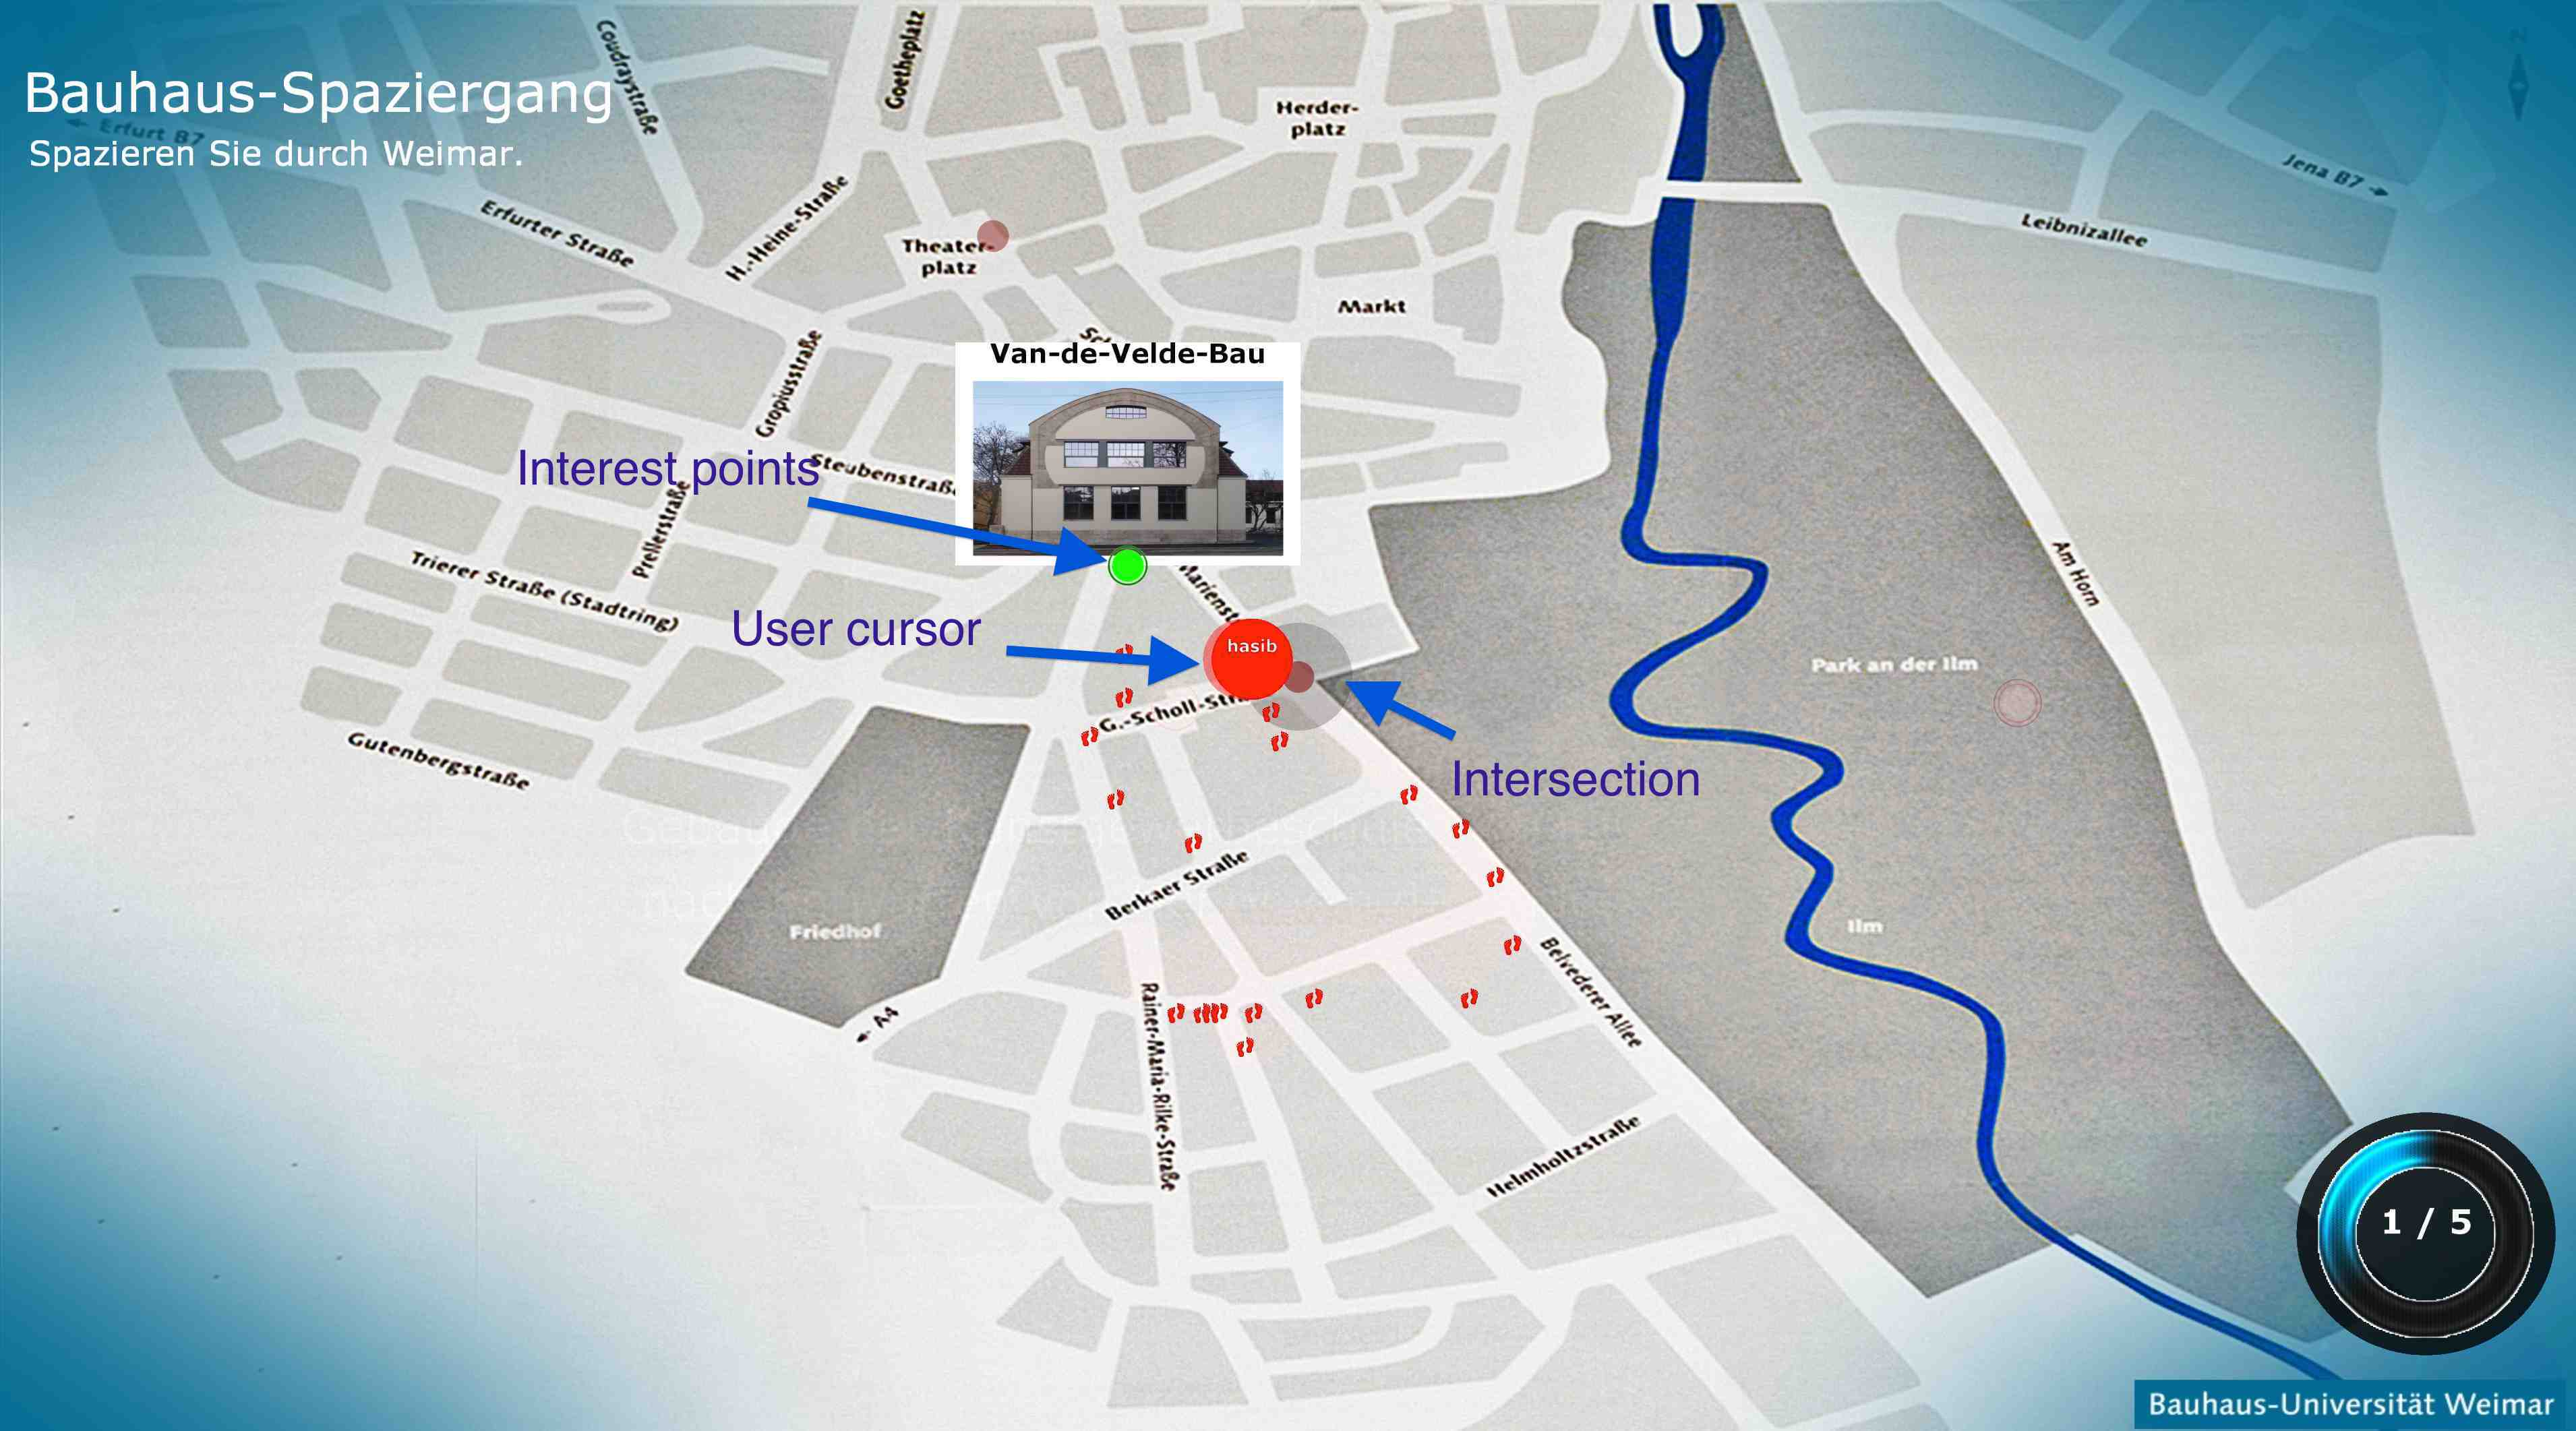
\includegraphics[width=0.8\textwidth,height=70mm]{Figures/7/mobile_interactive/second_interface}
    \caption{Map interface}%
    \label{fig:mobile_secondinterface}%
\end{figure}

\item Advertisement video:\\
The same advertisement video used for non-interactive is shown after the interaction is completed.


\item Mobile interface: \\
The interaction controller in the smartphone is shown below. The interface is very simply designed and has two elements, the cursor and the select button. With the cursor, the user can navigate inside the map to interest points and on reaching on an interest point the participant presses the select button to explore that location. 

\begin{figure}[H]
    \centering
    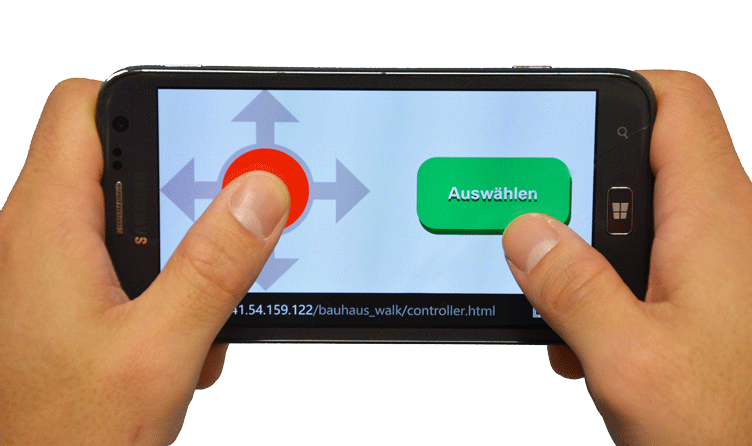
\includegraphics[width=100mm,height=60mm]{Figures/7/mobile_interactive/mobile_interface}
    \caption{Mobile controller}%
    \label{fig:mobile_controllerinterface}%
\end{figure}

\end{enumerate}

\iffalse

\subsubsection{Hardware setup}
The hardware required for the type of interactive application, would be to use one Access point that enable participants to connect to the system, Kinect camera to record colored user images, a mobile phone at client side and obviously the screen and a workstation.


\begin{figure}[H]
    \centering
    \includegraphics[width=100mm,height=60mm]{Figures/7/mobile_interactive/Mobile_hardware_setup}
    \caption{Hardware setup}%
    \label{fig:mobile_hardware_setup}%
\end{figure}


\subsubsection{Software setup}
In order to make the system running we would need the below things.
\hilight{The controller is taken from another project MMM ball}
\begin{itemize}
\item Apache webserver:\\
The web server could be running in the same application system side-by-side. The web controller is using WebSocket client at the backend. Check the JavaScript configuration
file to have the IP address configured where application system is using.
\item Processing and WebSocket:\\
The application should be started and along that the WebSocket server should also be running silmultaniously. Processing should have WebSocket library installed before hand. The system should have a valid IP address to be reached by webserver.
\item OpenProcessing Library:\\
Processing should have OpenProcessing library installed to be able to run Kinect Camera for color image recording.
\end{itemize}


\begin{figure}[H]
    \centering
    \includegraphics[width=120mm,height=60mm]{Figures/7/mobile_interactive/mobile_software}
    \caption{System architecture}%
    \label{fig:mobile_software_setup}%
\end{figure}

To have a full look to the software, please refer to the DVD to see all the source codes and the relavent applications.

\subsubsection{Flowchart Diagram}
The below chart roughly shows the flow of the application.
\begin{figure}[H]
    \centering
    \includegraphics[width=130mm,height=160mm]{Figures/7/mobile_interactive/mobile_flow_chart}
    \caption{Mobile Interactive advertisement Flowchart diagram}%
    \label{fig:mobile_flowchat}%
\end{figure}
\fi

\section{Interaction Design}
The body interaction model is designed based on \emph{Audience funnel},  a it suites well for public setups like the Tourist information center and advertising. With the design of this interaction model different levels of interactions and phases can be observed. Based on this model the three phases of the applications were designed (\emph{Call-to-Action}, Interaction interface and ad video). This model attracts passersby and gradually motivates them toward the display to engage them in interaction and at the same time it is also convenient for the passersby to avoid the display


\subsection{Body Interaction Design}
The diagram below shows the display at the top, the body-tracking area illustrated by a triangle. This triangle is divided into two sections that is separated by dashed lines, (1) gray region defines the least interest regions, because in this area it is assumed that people maybe busy with other things around the display, and people in this region can easily avoid the display and the display will not motivate them for interaction, and (2) the highest interest region, it is assumed that people are aware of the display and the display would motivate them for interactions only if they are facing towards display.


\begin{figure}[H]
    \centering
    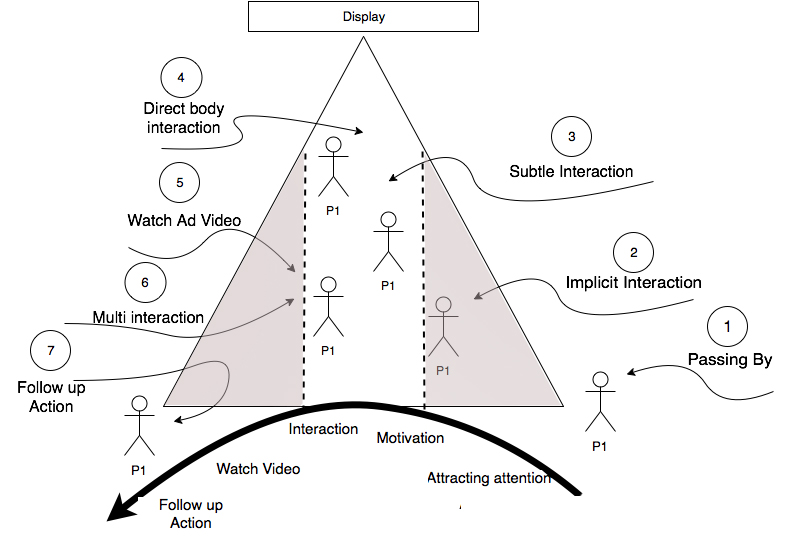
\includegraphics[width=0.9\textwidth,height=8cm]{Figures/7/body_interaction_model}
    \caption{Body interaction design.}%
    \label{fig:body_interaction_deisng}%
\end{figure}


The model consists of seven phases, each of them are explain in the following list.

\begin{enumerate}
\item \emph{Passing by phase:} \\
This phase demonstrates passersby, who are not in the display tracking range.

\item \emph{Implicit Interaction phase:} \\
This phase starts, when passersby are in tracking range but are standing far or at side of the display. 

\item \emph{Subtle interaction phase:} \\
In this phase, the user is in near or center area of tracking range and facing toward display. The system motivates the user for direction interaction with the \emph{Call-to-Action} feature (``\emph{To play, Come near}'').

\item \emph{Direct body interaction phase:} \\
This phase happens, when the user has actively started the game interaction and is playing. At this phase the whole tracking range (gray and white color) could be used for direct interaction until the end of interaction phase.

\item \emph{Watch ad video phase:} \\
When the interaction is over, a short advertisement video is shown.

\item \emph{Multi interaction phase:} \\
This phase demonstrates that the user can perform interaction multiple times.

\item \emph{Follow up action phase:} \\
Follow up action phase is, when the user leaves the display’s tracking range and performs other actions.

\end{enumerate}


The Black curve below the diagram shows the transition of the user between each phase and shows the flow of the attention, motivation, interaction and other phases. The attention is captured mainly in \emph{Implicit interaction phase}, the motivation occurs when the user is in \emph{Subtle interaction phase} and the interaction is when the user is directly playing with the his/her silhouette in the entire tracking coverage area. After the interaction and watching ad video, the curve changes direction moving down, which illustrates that the user would likely leave the interaction area and follow other actions unrelated to the screen. 

\begin{itemize}

\item Attention: \\
A \emph{Bottom-Up} approach was used to achieve the passersby attention because the approach can help get attention by showing a sudden object, or by contrasting various colors. To do so, the silhouette representation of passersby were projected on the screen, this representation can bring higher level of attraction as it is responsive to the user movements, and has different contrast colors in relation to background. In chapter 3, this method was compared with other forms of representation and attracting attention and the silhouette was the top candidate.

\item Motivation: \\
The motivation is done by bring joy, fun, curiosity and challenge\cite{ toward_motivation} to the users who are attracted toward thedisplay. In body interaction design the use of passersby’s silhouette presentation would be a good motivational force to bring passersby near the display. This technique can become a source of fun and entertainment and can give a sense of connectedness with the display. And at the same time it also motivates passersby by showing a \emph{Call-to-Action} message like “to play! Come near”, which is responsive to user movement and gives them confidence to play.

\item Interaction and follow up actions: \\
When the user starts the interaction, the interaction being carried out should be meaningful, understandable and easy, else the user will leave immediately after some tries. Therefore many focus groups and evaluations of many prototypes were conducted to assure the usability of the body interaction. The interaction is explained in detail in the previous sections.
After the end of the interaction, the advertisement video is shown and then the user can start again interaction or leave the screen.
\end{itemize}


\subsection{Mobile Interaction Design}
Below diagram shows the mobile interaction design. The diagram shows the display at the top, and the triangle represents body-tracking range for passersby. The design has the same 8 phases as proposed for the body interaction. (1) Passing by phase, which demonstrates passersby who are not in display tracking range, (2) Implicit Interaction phase, the mobile version also has the implicit body interaction for attracting attention only and it is not limited to a certain region, but the whole the tracking area could be used for this purpose, and no further direct interaction is possible, (3) Read Access info, after the user is attracted toward the screen, the user reads how to use his/her mobile phone to connect to the display, (4) connect to system, in this phase the user connects to Wi-Fi and opens the controller, (5) direct interaction phase, is when the user actively interacts using smartphone with the display, (6) Watch ad video, this phase is triggered when the interaction is over, (7) multi interaction phase, demonstrates that the user can perform interaction multiple times, (8) Follow up action phase, is when the user leaves the display’s tracking range and performs other actions.

\begin{figure}[H]
    \centering
    \includegraphics[width=0.9\textwidth,height=8cm]{Figures/7/mobile_interaction_design.png}
    \caption{Body interaction design.}%
    \label{fig:body_interaction_deisng}%
\end{figure}


\begin{enumerate}

\item Attention: \\
Technologies like Bluetooth, infrared and NFC\footnote{NFC: Near Field Communication} of mobile devices in fact could be used for attracting attention of passersby, but these technologies have their limitations and limited usage and not all mobile phones support all of the technologies. At the same time it is possible that the passersby have not switched on these technologies because of battery consumption or other purpose. Therefore to attract all the passersby without any limitation, the silhouette representation was used as it was used for body interaction design.

\item Motivation: \\
The motivation is also similar to the body interaction. Due to the display of the silhouette, it brings curiosity and joy to the users. Besides that, an Information text is shown on the screen to give sufficient information on how to access the advertisement system and play the game.

\item Interaction and follow up actions: \\
The interaction with the game element is only possible with the use of a smart phone. The interaction usability is important in order to keep the passersby engaged with the display. Therefore two prototype versions of the mobile interactions were evaluated to remove any possible usability issue. After the interaction is over the advertisement video and other following up action is taken on user.


\end{enumerate}



\section{Technical details}
The application is developed in Processing language with the support of Kinect Library. The application can run in Windows and OSX operating systems the system should have below requirements.


\begin{enumerate}
\item \textbf{Software Requriements:}

\begin{itemize}
\item \textbf{Processing v2.2.2.} \\
Website link: \url{https://processing.org/}

\item \textbf{Microsoft Kinect SDK} \\
Download link: \url{https://www.microsoft.com/en-us/download/details.aspx?id=40278}

\item \textbf{SimpleOpenNI} library for Processing. \\
Documentation link: \url{file:///Users/hcilab-mac2/Documents/Processing/libraries/SimpleOpenNI/documentation/SimpleOpenNI/SimpleOpenNI.html} 

\item \textbf{OpenKinect} processing. \\
Documentation: \url{http://shiffman.net/p5/kinect/}

\item \textbf{64bit JRE} (Java Runtime Environment) v1.8 or higher. \\
Download link: \url{http://www.oracle.com/technetwork/java/javase/downloads/jre8-downloads-2133155.html}

\item \textbf{Windows / Mac OSX} Operating system.

\end{itemize}


See Appendix \ref{app:fileandfolders} for more details.

\item \textbf{Hardware Requriements:}

\begin{itemize}
\item \textbf{RAM:} 4GB or above.
\item \textbf{CPU:} Core i5 / i7 2.3Ghz
\item \textbf{Kinect V1 camera} \\
Documentation link: \url{https://msdn.microsoft.com/en-us/library/jj131033.aspx}

\end{itemize}


\end{enumerate}

\subsection{Body Interactive}

\subsubsection{Silhouette representation}
The reason behind silhouette representation of passersby was to attract their attention toward the display. There are a lot of body sensing technologies, and the most easy way was to use Microsoft Kinect camera\footnote{Microsoft Kinect: https://developer.microsoft.com/de-de/windows/kinect, last accessed 5 jun 2016}, that has built-in algorithm to track people. The camera has a resolution of 640x480 pixels. I created the colored silhouette representation from the \emph{UserMap} array sent by the camera, which was a 1xD integer array that corresponds to the pixels of the image. The array looks like below \\

\emph {Int upix = context.userMap();}

\emph{upix = [1,1,1,1,1,1,1,2,2,2,2,2,2,2,2,2,-1,-1,-1,-1,-1,-1,2,2,2,2,....]}

The above example shows the structure of the array, the index of the elements of the array correspond to the pixel number of image, and the element values correspond to the user ID tracked by the camera. The user ID is always above zero, any value that is not above zero could be related to background or non-user pixel. The example shows that there are at least two people standing in front of the camera, which have user ID (1 and 2), the -1 value is a non-user pixels. 
So the application iterates to this array and assigns specific color to each of the pixels of the user image, and does not give color to the non-user pixels. After assigning the color value to each user in the picture and leave out the background as null, the below picture will be created.




% If you use beamer only pass "xcolor=table" option, i.e. \documentclass[xcolor=table]{beamer}
\begin{table}[H]
\centering
\caption{UserMap and application color mapping}
\label{usermap_colormapping}
\resizebox{0.8\textwidth}{3cm}{ 
\begin{tabular}{ccccccccccccccccccccccccccccccccccccccccc}
-1 & -1 & -1                        & -1                        &                           &                           &                           &                           &                           &                           &                           &                           &                           &                           &                           &                           &                           &                           &                           &                           &                           &                           &                           &    &    &    &                           &                           &                           &                           &                           &                           &                           &                           &                           &                           &                           &                           &  &  &  \\
-1 & -1 & -1                        &                           & -1                        &                           & -1                        & -1                        & -1                        &                           & -1                        & -1                        & -1                        & -1                        & -1                        & -1                        & -1                        & -1                        & -1                        & -1                        &                           &                           &                           &    &    &    &                           &                           & -1                        &                           & -1                        &                           & -1                        & -1                        &                           &                           &                           &                           &  &  &  \\
   &    &                           &                           &                           &                           &                           &                           &                           &                           &                           &                           &                           &                           &                           & -1                        &                           &                           &                           &                           &                           &                           &                           & -1 &    &    & -1                        & -1                        & -1                        & -1                        &                           & \cellcolor[HTML]{FE0000}2 & -1                        & -1                        & -1                        &                           &                           &                           &  &  &  \\
-1 & -1 & -1                        & -1                        & -1                        & -1                        & -1                        & -1                        & -1                        & -1                        & -1                        & -1                        & -1                        & -1                        &                           &                           &                           &                           & -1                        &                           &                           &                           &                           &    &    &    & \cellcolor[HTML]{FE0000}2 & -1                        & -1                        &                           & \cellcolor[HTML]{FE0000}2 & \cellcolor[HTML]{FE0000}2 & \cellcolor[HTML]{FE0000}2 & -1                        & -1                        & \cellcolor[HTML]{FE0000}2 &                           &                           &  &  &  \\
-1 & -1 & -1                        & -1                        & -1                        & -1                        & -1                        & -1                        & -1                        & -1                        & -1                        & -1                        & -1                        & -1                        & -1                        & -1                        &                           &                           &                           &                           &                           &                           &                           &    &    &    &                           & \cellcolor[HTML]{FE0000}2 & \cellcolor[HTML]{FE0000}2 & \cellcolor[HTML]{FE0000}2 & \cellcolor[HTML]{FE0000}2 & \cellcolor[HTML]{FE0000}2 & \cellcolor[HTML]{FE0000}2 & \cellcolor[HTML]{FE0000}2 & \cellcolor[HTML]{FE0000}2 &                           &                           & -1                        &  &  &  \\
-1 & -1 & -1                        & -1                        & -1                        & -1                        & -1                        & -1                        & -1                        & -1                        & -1                        & -1                        & -1                        & -1                        & -1                        &                           &                           &                           &                           & -1                        &                           &                           &                           &    &    &    &                           & -1                        & -1                        & -1                        & \cellcolor[HTML]{FE0000}2 & \cellcolor[HTML]{FE0000}2 &                           & -1                        & -1                        & -1                        &                           &                           &  &  &  \\
-1 & -1 & -1                        & -1                        & -1                        & -1                        & -1                        & -1                        &                           &                           & -1                        &                           & -1                        &                           &                           & -1                        &                           &                           &                           &                           & -1                        &                           &                           &    &    &    &                           &                           &                           &                           & \cellcolor[HTML]{FE0000}2 & \cellcolor[HTML]{FE0000}2 &                           &                           &                           & -1                        &                           &                           &  &  &  \\
   &    &                           &                           &                           &                           &                           &                           &                           &                           &                           &                           &                           &                           &                           &                           &                           & -1                        & -1                        &                           &                           &                           &                           &    &    &    &                           &                           &                           & \cellcolor[HTML]{FE0000}  & -1                        & -1                        & \cellcolor[HTML]{FE0000}2 &                           &                           &                           &                           & -1                        &  &  &  \\
   &    &                           &                           &                           &                           &                           &                           &                           &                           &                           &                           &                           &                           &                           &                           &                           & -1                        & -1                        &                           &                           &                           &                           &    &    &    &                           &                           & \cellcolor[HTML]{FE0000}2 & -1                        & -1                        & -1                        & -1                        & \cellcolor[HTML]{FE0000}2 &                           &                           &                           &                           &  &  &  \\
   &    &                           &                           &                           &                           &                           &                           &                           &                           &                           & \cellcolor[HTML]{3531FF}3 & \cellcolor[HTML]{3531FF}3 & \cellcolor[HTML]{3531FF}3 & -1                        &                           &                           & -1                        & -1                        &                           &                           &                           &                           &    &    &    &                           & \cellcolor[HTML]{FE0000}2 & \cellcolor[HTML]{FE0000}2 &                           & -1                        & -1                        &                           &                           & \cellcolor[HTML]{FE0000}2 &                           &                           &                           &  &  &  \\
   &    & \cellcolor[HTML]{3531FF}3 &                           &                           &                           &                           &                           &                           &                           &                           & \cellcolor[HTML]{3531FF}3 & \cellcolor[HTML]{3531FF}3 & \cellcolor[HTML]{3531FF}3 & -1                        &                           & -1                        & -1                        & -1                        &                           &                           & \cellcolor[HTML]{3531FF}3 & \cellcolor[HTML]{3531FF}3 &    &    &    &                           &                           &                           &                           &                           &                           &                           &                           &                           &                           &                           &                           &  &  &  \\
   &    &                           & \cellcolor[HTML]{3531FF}3 & \cellcolor[HTML]{3531FF}3 &                           &                           &                           &                           &                           &                           &                           & \cellcolor[HTML]{3531FF}3 & \cellcolor[HTML]{3531FF}3 & -1                        & -1                        & -1                        &                           &                           & \cellcolor[HTML]{3531FF}3 & \cellcolor[HTML]{3531FF}3 & -1                        &                           & -1 & -1 & -1 &                           &                           &                           & -1                        &                           & -1                        & -1                        &                           & -1                        &                           & -1                        &                           &  &  &  \\
   &    &                           &                           &                           & \cellcolor[HTML]{3531FF}3 & \cellcolor[HTML]{3531FF}3 & \cellcolor[HTML]{3531FF}3 & \cellcolor[HTML]{3531FF}3 & \cellcolor[HTML]{3531FF}3 & \cellcolor[HTML]{3531FF}3 & \cellcolor[HTML]{3531FF}3 & \cellcolor[HTML]{3531FF}3 & \cellcolor[HTML]{3531FF}3 & \cellcolor[HTML]{3531FF}3 & \cellcolor[HTML]{3531FF}3 & \cellcolor[HTML]{3531FF}3 & \cellcolor[HTML]{3531FF}3 & \cellcolor[HTML]{3531FF}3 &                           &                           &                           &                           &    &    &    &                           & -1                        & -1                        & -1                        & -1                        & -1                        & -1                        & -1                        & -1                        & -1                        & -1                        & -1                        &  &  &  \\
   &    & -1                        &                           &                           &                           &                           &                           &                           & \cellcolor[HTML]{3531FF}3 & \cellcolor[HTML]{3531FF}3 & \cellcolor[HTML]{3531FF}3 & \cellcolor[HTML]{3531FF}3 & \cellcolor[HTML]{3531FF}3 & \cellcolor[HTML]{3531FF}3 & \cellcolor[HTML]{3531FF}3 & \cellcolor[HTML]{3531FF}3 &                           &                           &                           &                           &                           & -1                        &    &    &    &                           &                           &                           &                           &                           &                           &                           &                           &                           &                           &                           &                           &  &  &  \\
   &    &                           &                           &                           &                           &                           &                           &                           &                           & \cellcolor[HTML]{3531FF}3 & \cellcolor[HTML]{3531FF}3 & \cellcolor[HTML]{3531FF}3 & \cellcolor[HTML]{3531FF}3 & \cellcolor[HTML]{3531FF}3 & \cellcolor[HTML]{3531FF}3 &                           & -1                        &                           & -1                        &                           &                           & -1                        & -1 & -1 &    & \cellcolor[HTML]{329A9D}1 &                           &                           &                           &                           & \cellcolor[HTML]{329A9D}1 & \cellcolor[HTML]{329A9D}1 &                           &                           &                           &                           & \cellcolor[HTML]{329A9D}1 &  &  &  \\
   & -1 &                           &                           &                           &                           &                           &                           &                           &                           & \cellcolor[HTML]{3531FF}3 & \cellcolor[HTML]{3531FF}3 & \cellcolor[HTML]{3531FF}3 & \cellcolor[HTML]{3531FF}3 & \cellcolor[HTML]{3531FF}3 & \cellcolor[HTML]{3531FF}3 &                           &                           &                           &                           &                           &                           & -1                        &    &    &    & \cellcolor[HTML]{329A9D}1 & \cellcolor[HTML]{329A9D}1 & \cellcolor[HTML]{329A9D}1 & \cellcolor[HTML]{329A9D}1 & \cellcolor[HTML]{329A9D}1 & \cellcolor[HTML]{329A9D}1 & \cellcolor[HTML]{329A9D}1 & \cellcolor[HTML]{329A9D}1 & \cellcolor[HTML]{329A9D}1 & \cellcolor[HTML]{329A9D}1 & \cellcolor[HTML]{329A9D}1 &                           &  &  &  \\
   &    &                           &                           &                           &                           & -1                        &                           &                           &                           & \cellcolor[HTML]{3531FF}3 & -1                        & -1                        & -1                        & \cellcolor[HTML]{3531FF}3 & \cellcolor[HTML]{3531FF}3 &                           &                           &                           &                           &                           &                           & -1                        &    & -1 &    &                           & -1                        &                           & -1                        & \cellcolor[HTML]{329A9D}1 & \cellcolor[HTML]{329A9D}1 & \cellcolor[HTML]{329A9D}1 & \cellcolor[HTML]{329A9D}1 &                           &                           &                           &                           &  &  &  \\
   &    &                           &                           &                           &                           &                           &                           &                           &                           & \cellcolor[HTML]{3531FF}3 & -1                        & -1                        & -1                        & \cellcolor[HTML]{3531FF}3 & \cellcolor[HTML]{3531FF}3 &                           &                           &                           &                           &                           &                           & -1                        &    &    &    &                           &                           &                           &                           & \cellcolor[HTML]{329A9D}1 & \cellcolor[HTML]{329A9D}1 & \cellcolor[HTML]{329A9D}1 & \cellcolor[HTML]{329A9D}1 &                           &                           &                           & -1                        &  &  &  \\
   &    &                           &                           &                           &                           &                           &                           &                           &                           & \cellcolor[HTML]{3531FF}3 & -1                        & -1                        & -1                        & \cellcolor[HTML]{3531FF}3 & \cellcolor[HTML]{3531FF}3 &                           &                           &                           &                           &                           &                           & -1                        &    &    &    & -1                        & -1                        &                           &                           & \cellcolor[HTML]{329A9D}1 & -1                        & -1                        & \cellcolor[HTML]{329A9D}1 &                           &                           &                           &                           &  &  &  \\
   &    &                           &                           &                           &                           &                           &                           & \cellcolor[HTML]{3531FF}3 & \cellcolor[HTML]{3531FF}3 & \cellcolor[HTML]{3531FF}3 & -1                        & -1                        & -1                        & \cellcolor[HTML]{3531FF}3 & \cellcolor[HTML]{3531FF}3 &                           &                           &                           &                           &                           &                           &                           &    &    &    &                           &                           &                           &                           & \cellcolor[HTML]{329A9D}1 & -1                        & -1                        & \cellcolor[HTML]{329A9D}1 &                           &                           &                           &                           &  &  & 
\end{tabular}
}
\end{table}

The above picture has very limited pixels. It is not an original picture but is made to clear the idea of how the coloring of silhouette works. From the above picture, the white areas or the -1 values are background and non-user and the remaining positive numbers represent the pixels related to the user.
Check the Silhouette video\footnote{Attraction attention method: \url{https://www.youtube.com/watch?v=1EtHVqS412M}, last accessed 5 jun 2016}. For more information about the source codes, please refer Appendix \ref{app:fileandfolders} to find the source files in the DVD.



\subsection{Mobile interactive}


\subsubsection{Requirements}
\begin{itemize}
\item \textbf{Apache webserver:}\\
The web server is running mobile web controller. It is using \emph{WebSocket} client at the backend. I used \emph{XAMPP} server for windows in which the Apache server was running. 

XAMPP website link: \url{https://www.apachefriends.org/de/index.html}  \\

\item \textbf{WebSocket:}\\
Mobile interactive advertisement application and \emph{WebSocket} application should be running simultaneously.  \\
Websocket website link: \url{https://www.websocket.org/}

\item \textbf{Access point}\\
An access point is necessary to allow mobile users connect to the webserver. The access point should distribute from the same range of IP addresses to clients as the advertisement application has.


Check Appendix \ref{app:fileandfolders} for more details.

\end{itemize}

\subsubsection{Software setup}

\begin{figure}[H]
    \centering
    \includegraphics[width=120mm,height=60mm]{Figures/7/mobile_interactive/mobile_software}
    \caption{System architecture}%
    \label{fig:mobile_software_setup}%
\end{figure}


\subsubsection{Hardware setup}
The hardware required for mobile interactive application, is to use one \emph{Access point} that enable participants to connect to the system, and a \emph{Kinect} camera to record colored user images. See the below hardware diagram.

\begin{figure}[H]
    \centering
    \includegraphics[width=0.8\textwidth,height=70mm]{Figures/7/mobile_interactive/Mobile_hardware_setup}
    \caption{Hardware setup}%
    \label{fig:mobile_hardware_setup}%
\end{figure}














% Chapter 6
\chapter{Advertisement High Fidelity prototype} % Main chapter title

\label{Chapter6} % For referencing the chapter elsewhere, use \ref{Chapter1} 

\newpage

\section{Introduction}
A follow up study is conducted when a final version of a prototype is ready. A \emph{summative} ``\emph{is used to evaluate how well the design meets the usability requirements}''\cite{summative}. It is to finalize the decisions on a prototype, there have been studies like ``\emph{Sweep and point \& shoot}'' \cite{SweepPointShoot} that evaluated prototypes for interaction of personal computing device with large public displays. Another evaluation was of ``\emph{mobile interaction with live video}'' \cite{TouchProjector} that used a with-in subject design, where the participant’s performance were measured for automatic zooming and temporary image freezing. Sebastian .D \cite{WalldragandDrop} assessed the general performance of drag and drop interaction on large displays and compared it with a traditional drag and drop. Jorg Müller \cite{LookingGlass} did pre-studies (lab and field) on noticing interactivity of a display in which the time required for recognizing interactivity by participants were measured.

Based on the feedbacks from the low-fidelity evaluation in the previous chapter, I developed two functional hi-fidelity version of interactive advertisement of the body and mobile. This chapter explains the evaluation process of the Hi-fidelity prototypes of interactive advertisement both body and mobile. The evaluations were more on user performance, user acceptance and usability issues. As the application would be in public, where many people would interact, the application performance was also tested with single and multi-users to ensure application stability.


\section{Advertisement prototypes}
The prototype was to show a city map on the screen with possible interactive famous places of Bauhaus. The interaction idea was to map physical movement of the user, or map the cursor movement of a phone to the virtual movement on the city map. The interaction let users to explore the target places by reaching those locations. Five places were to be explored by one person to complete the interaction.


In this prototype there were mainly three hierarchical levels of interfaces, (1) \emph{Call-to-Action}, (2) \emph{Game interaction}, and (3) the advertisement video interface.

\begin{itemize}
\item \emph{Call-to-Action} interface: \\
This interface invites participants to interact with the application. This method was first proposed by Bill Kules \cite{call-to-action}, in which the immediate usability of public accesses to a system was designed. \emph{Call-to-Action} of body and mobile are designed differently, which are shown in below sections. 

\item Interaction interface: \\
This interface activates when the user follows the instructions of the first interface, the interface shows the interactive map with the hotspots to be explored by participants.

\item Video advertisement: \\
After the interaction is completed then a silent video advertisement is shown for 20 seconds. 
The advertisement video was created in powtoon\footnote{Powtoon: \url{https://www.powtoon.com}, last accessed: 21 April 2016} with a free version account, to see the full advertisement video visit below these videos, video1\footnote{Old video version: \url{https://www.youtube.com/watch?v=GrWtOyjNcQ0}} and video2\footnote{ New video version: \url{https://www.youtube.com/watch?v=-y1Dbz6E6bU&feature=youtu.be}}

\end{itemize}


\newpage
\subsection{Body prototype}
This section introduces the interfaces of the body interactive prototype and the processes of how a user can start interaction. Watch this demo video\footnote{Body interaction: \url{https://www.youtube.com/watch?v=Uhvn43gImmk}, last accessed: 29 June 2016} to have a short glance to the interactions.

\begin{enumerate}

\item \emph{Call-to-Action} interface: \\
This interface is basically attraction attention and \emph{Call-to-Action}interface. As you can see below picture, there is someone standing in front of the screen and the interface calls the person to come near. This interface also has alert message section on the top right that alerts the participant if moved away from the camera range. 

\begin{figure}[H]
    \centering
    \includegraphics[width=120mm,height=70mm]{Figures/6/body/first_interface}
    \caption{call-to-action interface}%
    \label{fig:body_firstinterface}%
\end{figure}

When a new person steps in the range of the camera, his/her silhouette is projected on the screen with a different color, and then the application calls the person to come near in order to trigger the game.


\item Transition to interaction interfaces: \\
The transition happens when the person stands close to the screen for more than 3 seconds and the below things happen.

\begin{enumerate}
\item Loading animation:\\
 The loading animation is a reaction to the action of the participants, which gives the user a clue that the interaction will be started. 

\item Scaling down the silhouette: \\
The participant's silhouette is scaled down to allow him/her to walk freely on the map and to give the participant the feeling of walking, 

\item Show task instruction:  \\
Every interaction has an instruction, the instruction is fairly very easy and it is simplified in one sentence as, ``\emph{To play, come near}''.
\end{enumerate}

\begin{figure}[H]
    \centering
    \begin{subfigure}[H]{0.3\textwidth}
        \centering
        \includegraphics[width=\textwidth,height = 3.5cm]{Figures/6/body/loading}
        \caption{Loading}
        \label{fig:loading_logo}
    \end{subfigure}
    \begin{subfigure}[H]{0.3\textwidth}
        \centering
        \includegraphics[width=\textwidth,height = 3.5cm]{Figures/6/body/scalling_down}
        \caption{Scalling down}
        \label{fig:scalling_down}
    \end{subfigure} 
      \begin{subfigure}[H]{0.3\textwidth}
        \centering
        \includegraphics[width=\textwidth,height = 3.5cm]{Figures/6/body/task_description}
        \caption{Task description}
        \label{fig:task_description}
    \end{subfigure}
    \caption{Transitions of interfaces }
    \label{fig:transition_sequence}
\end{figure}


\item Interaction interface: \\
In this interface, participants can interact with the elements on the map. As shown in the picture below, the silhouette has visited four locations and has a score of 4 out of 5. In order to finish the interaction the user needs to visit the last location.

\begin{figure}[H]
    \centering
    \includegraphics[width=130mm,height=80mm]{Figures/6/body/interaction_inter}
    \caption{Second Interface}%
    \label{fig:body_secondinterface}%
\end{figure}

%\subsubsection{Flowchart Diagram}
%The below chart roughly shows the flow of the application.
%\begin{figure}[H]
%    \centering
%    \includegraphics[width=120mm,height=140mm]{Figures/7/body_interactive/body_flow_chart}
%    \caption{Body Interactive advertisement Flowchart diagram}%
%    \label{fig:Body_flowchat}%
%\end{figure}

\end{enumerate}

\subsection{Mobile}
Mobile interaction is possible by using a smartphone and a Wi-Fi connection to the advertisement network. The user should open the mentioned IP address in his / her mobile browser and enter a name to login. After login, a mobile controller appears by which the user can control the map elements on the screen. Watch this demo video\footnote{Mobile interaction: \url{https://www.youtube.com/watch?v=ooxWjgd0xUs}, last accessed: 29 June 2016} to have a short glance to interactions.

\begin{enumerate}

\item \emph{Call-to-Action} interface: \\
This interface is designed in such a way to attract passers-by and also guide the participants on how to use their smartphone to access the advertisement application. The attraction is again the same method that was used for the body, the passers-by silhouette is projected at the back of the Access information. The interface has a QR code that could be easy to be scanned instead of typing the whole IP address. There is an alert area that gets activated when a person is logged in and has not changed the orientation of the phone to landscape.

\begin{figure}[H]
    \centering
    \includegraphics[width=120mm,height=70mm]{Figures/6/mobile/call-to-action}
    \caption{Mobile interactive interface:}%
    \label{fig:mobile_firstinterface}%
\end{figure}



\item Transition to interaction interfaces: \\
The transition happens only when the user connects to the Wi-Fi, open the controller and physically holds the phone in landscape.

\begin{enumerate}
\item Loading animation:\\
The loading animation is a reaction to the action of the participants, which gives the user a clue that the interaction will be started. 
\item  Creating Colored cursor: \\
A colored circle is created for the participant in the center of the screen. Each participant has different color matching to his/her controller interface in his or her phone.
\item Show task instruction:  \\
The instruction is fairly very easy and it is simplified in one sentence to explore locations on the map by using their phone.


\end{enumerate}


\begin{figure}[H]
    \centering
    \begin{subfigure}[H]{0.45\textwidth}
        \centering
        \includegraphics[width=\textwidth,height=4cm]{Figures/6/mobile/loading}
        \caption{Loading}
        \label{fig:loading_mobile}
    \end{subfigure}
    \begin{subfigure}[H]{0.45\textwidth}
        \centering
        \includegraphics[width=\textwidth,height=4cm]{Figures/6/mobile/task_desc}
        \caption{Task description}
        \label{fig:task_mobile}
    \end{subfigure}
    \caption{Transitions of interfaces.}
    \label{fig:Switching_between_phases_mobile}
\end{figure}


\item Interation interface \\
The second screen is the interaction screen for the participants. The participants can navigate the cursor using their phone controller page. It can be seen in the below picture, the user is controlling the cursor and has explored one location. The user's defined name is also shown on the cursor so that the user do not lose track of his/her cursor. A small circle around the target location is shown is to determine the area of intersection. The interaction completes when all the locations are explored or the interaction time has finished.

\begin{figure}[H]
    \centering
    \includegraphics[width=120mm,height=70mm]{Figures/6/mobile/interaction_inter}
    \caption{Mobile interactive interface}%
    \label{fig:mobile_secondinterface}%
\end{figure}



\item Mobile interface: \\
This interface was designed by a student project called \emph{MMM Ball} \cite{MMMball, MMMball2} in Bauhaus University.
When the user opens the webpage and enters his/her name, the below interface would appear. The interface is simply designed and has two elements, the cursor and the select button. With cursor the user can navigate inside the map to reach target locations and then presses the select button to explore that location.

\begin{figure}[H]
    \centering
    \includegraphics[width=100mm,height=60mm]{Figures/6/mobile/mobile_interface}
    \caption{Mobile controller interface: The left side is the cursor and the right side is the select button.}%
    \label{fig:mobile_controllerinterface}%
\end{figure}


\end{enumerate}

\section{Research questions}

\begin{enumerate}
\item   How fast do users understand \emph{Call-to-Action}?
\item   How fast participants react to the \emph{Call-to-Action}?
\item   How easy it is for the participants to understand the interaction task?
\item   How long does it take for the participants to complete the interaction or visit all the target locations?
\item   What are the major usability flaws that prevent users from advertisement interactions?
\item   What is the difference between mobile and body performance?
\item   How the applications would perform in single user interaction and in multi user interaction?

\end{enumerate}

\subsection{Video advertisement}
\begin{enumerate}
\item   Do participants understand the content of the advertisement?
\item   How many elements of display can participants recall after their first interaction?
\end{enumerate}


\section{Test Design}
This study used a within subject design, in which each participants were asked to experience with both body and mobile prototypes. The interaction sequence was interchanged for participants in order to counterbalance the learning effect.

\subsection {Participants}
12 participants were invited for the usability testing, from which five participants were female and seven were male. Most of the participants had computer science background and were familiar with mobile and had seen or worked with body sensing technologies. All participants were familiar with QR code except one participant. 

\subsection{Task}
Participants were not told about any specific task, they were asked to explore the system by their own and understand the task. To avoid different outcomes participants were told to continue interaction until they encounter back with the first stage of the application. So the tasks for participants were to start from the initial stage of the interaction (body /mobile) and continue until they reach the initial stage again.

For body interaction, no extra device was required to accomplish the task, but for the mobile interaction a mobile phone was required. The participants were not told that the use of mobile is required unless they tried to use their own phone or asked for it from me.


\begin{itemize}

\item \textbf{Task understandability:} \\
Participants were told to \emph{Think-Aloud} on what task will they perform at each stage. 


\item \textbf{Performance measurment:} 
\begin{itemize}
\item \emph{Call-to-Action} understanding duration \\
The time from when the user saw his/her silhouette until he/she understood / approached to start the interaction. For body \emph{Call-to-Action}, this duration is measured if the person intentionally moved toward the screen, and for mobile \emph{Call-to-Action}, when the person pulled the phone out.

\item Triggering game duration\\
This time is measured from the time the user understood how to start the interaction until the user actually starts the interaction. For example, in case of mobile interaction, the time is measured from the time the user takes out the mobile until he logins and opens the interaction controller.

\item Task understanding duration \\
This time is measured when the user starts the game until he/she understands the interaction task.

\item Task completion duration \\
Task completion time is measured from the time interaction starts until the interaction ends. 

\end{itemize}


\item \textbf{Content recall:} \\
After the first interaction with the advertisement, participants were immediately given a paper and a pen to write down the name of anything that they could recall. The interactions (mobile and body) were counterbalanced between the participants.

\item \textbf{Usability issues:} \\
Each participant was given five minutes to interact with both the mobile and the body advertisements. Then follow up questions were asked regarding the issues they faced. The usability issues like (confusing, unclear events and mistakes) were observed by the moderator at the scene and later while watching the recorded videos. 



\end{itemize}

\subsection{Data Gathering }
The below data were gathered.

\begin{itemize}

\item Performance data: \\
 The performance data of participants like, \emph{Triggering game duration}, \emph{Task understanding duration}, \emph{Task completion duration} and \emph{Whole interaction duration}was collected from both mobile and body interactions. To get an overview of performance in general the mean duration of the performance data were computed.

\item Preference data: \\
The preference data is the measures of participant opinion or thought process. The below preference data were collected.

\begin{itemize}

\item \emph{Think-Aloud} quotes \\
These quotes were noted during the video observation. These quotes were important to check at which time users understand about the interaction and tasks. 
It also helped to analyze their reaction and feedbacks toward the tasks being done.

\item Interview transcripts \\
All the interviews were transcribed and color-coding technique was applied to analyze and comprehend different aspects and categories from the defined questions.


\item Recordings \\
There were two different recordings done during the session, first was video recording using camera at the back of the room, that could record user actions and the computer screen and the second recording was the screen recoding of the application using \emph{QuickTIme} screen recorder. These recordings were used to analyze behavior, application performance and listen to the things participants said during interaction.


\end{itemize}



\begin{figure}[H]
    \centering
    \begin{subfigure}[H]{0.45\textwidth}
        \centering
        \includegraphics[width=\textwidth,height=4cm]{Figures/6/singleBody}
        \caption{Participant in body interaction mode.}
        \label{fig:singlebody}
    \end{subfigure}
    \begin{subfigure}[H]{0.45\textwidth}
        \centering
        \includegraphics[width=\textwidth,height=4cm]{Figures/6/singleMobile}
        \caption{Participant in mobile interaction mode}
        \label{fig:singleMobile}
    \end{subfigure}
    \caption{Participant's video recordings}
    \label{fig:Focus_group_room}
\end{figure}

\end{itemize}



\section{Findings}


\subsection{User performance}


\begin{itemize}

\item Mobile Interaction performance: \\
The chart shown below exhibits the performance data, when the participants used the mobile interaction.
The y-axis shows duration in seconds and x-axis shows the phases(aspects). You can see performance chart for each individual of mobile in Appendix \ref{app:mobile_performance}.




\begin{figure}[H]
\centering
\includegraphics[width=12cm,height=5cm]{Figures/6/mobile_average}%
 \caption{Chart that shows each aspect with respect to duration. }%
 \label{fig:mobile_average}%
\end{figure}

Participants took 49 seconds in average to understand \emph{Call-to-Action}. After participants understood what to do, it took 73 seconds in average to trigger the game (\emph{Triggering game duration}). It took 45 seconds in average to figure out how to do the task (\emph{Task understanding duration}) and 72 seconds to complete the task(\emph{Task completion duration}). As a result in average 240 seconds were taken for whole interaction time.
%
%\begin{figure}[H]
%\centering
%\includegraphics[width=12cm,height=6cm]{Figures/6/mobile_mean}%
% \caption{Confidence interval for Mobile interaction all phases duration }%
% \label{fig:mobile_mean}%
%\end{figure}

%above chart is generated in an online tool [1] with a confidence interval up to 95\% for complete interaction time for all 11 participants; the confidence interval is between (210.2, 267) the chart shows the Arithmetic standard deviation to be up to 38.82 seconds, Arithmetic Mean to be 240 seconds

\item Body Interaction performance: \\
The chart shown below exhibits the performance data, when the participants used the body interaction.
The y-axis shows duration in seconds and x-axis shows the phases(aspects). You can see performance chart for each individual of mobile in Appendix \ref{app:body_performance}.

\begin{figure}[H]
\centering
\includegraphics[width=12cm,height=5cm]{Figures/6/body_average}%
 \caption{Chart that shows each aspect with respect to duration}%
 \label{fig:body_average}%
\end{figure}

As can be seen above most of the participants finished the whole interaction in approximately 81 seconds, which is much better than mobile interaction. It took 6 seconds to understand \emph{Call-to-Action}. It took 5 seconds to trigger the interaction and start the game(\emph{Triggering game duration}). Participants took 23 seconds in average to understand the task (\emph{Task understanding duration}). And it took 47 seconds to complete the tasks(\emph{Task completion duration}).
%\begin{figure}[H]
%\centering
%\includegraphics[width=12cm,height=6cm]{Figures/6/body_mean}%
% \caption{Confidence interval for body interaction all phases duration }%
% \label{fig:body_mean}%
%\end{figure}

%The above confidence interval for body interaction is generated using the web tool [1] for whole body interaction time. In which with the confidence interval of 95\% is between (69.7 ? 91) seconds, with the standard deviation of 15.79 seconds.


\item Body Vs. Mobile performance: \\
The following graph shows that the body interaction is much better than the mobile interaction in terms of performance. The whole interaction time of body is less than the half of the time of mobile interaction. 

\begin{figure}[H]
\centering
\includegraphics[width=12cm,height=6cm]{Figures/6/mobile_body_performance}%
 \caption{Comparison of body and mobile interaction performance }%
 \label{fig:mobile_body_performance}%
\end{figure}

81 second was the mean value of the all the participants’ performance with body interaction and 240 seconds is the mean value of the same participants with mobile interaction. The following chart shows other comparison of each aspect as described.


\begin{figure}[H]
\centering
\includegraphics[width=12cm,height=6cm]{Figures/6/mobile_body_aspect}%
 \caption{Comparison of the aspects of interaction among body and mobile }%
 \label{fig:mobile_body_aspect}%
\end{figure}


The mobile interaction took much longer than body interaction for each phase or aspects, as \emph{ANOVA} revealed a strong significant difference of \emph{Call-to-Action} between body and mobile interaction ( \emph{(F1,11)=22.4758, p < .001 (p=.0001)}). A post-hoc Tukey test shows that participants understood very quickly the \emph{Call-to-Action} of body interaction compared to mobile interaction technique.

\emph{ANOVA} revealed a significant difference of triggering game between body and mobile interaction, ( \emph{(F1,11)=124.1066, p < .001}). Post-hoc Tukey test shows that in body interaction the triggering happens much faster than mobile interaction. 

\emph{ANOVA} revealed a significant difference of task understandability between body and mobile, ( \emph{(F1,11)=7.1340, p < .05 (p=.0147)}). A post-hoc Tukey test shows that participants understood the task very faster compared to mobile technique.

Interaction time was also significantly different as \emph{ANOVA} test strongly suggested a significant difference between the mobile and body interactions, ( \emph{(F1,11)=19.7000, p < .001 (p=.01)}). Post-hoc Tukey test strongly states that body interaction takes less time to complete the interaction compared to mobile.

\end{itemize}



\subsection{Usability issues}
The following usability issues are gathered from participant while observing them during the interactions.


\begin{itemize}

\item \textbf{Mobile Interaction:}
\begin{enumerate}
\item	Call-to-Action
\begin{enumerate}
\item At the first look of application, most participants did not read the text on the screen, they were expecting other way to get quick information. But after many tries with their body, they had to read the information text. 

\item   Participants did not understand about the phone icon or the browser animation on top of it until they figured by themselves.
\item   Frustration of typing the IP address.
\item   The size of QR code was small.
\end{enumerate}


\item   Use of mobile phone.
\begin{enumerate}
\item   In the beginning the participants did not except to use their own phone for the interactions; Many times participants asked, ``\emph{Should I use my phone?}'' 
\item   Most participants did not read the instruction to tilt their phone and even if they accidently had tilted the phone.
\item   There was no instruction to turn-on the tilt-sensor in the mobile phone.
\end{enumerate}

\item   Login page
\begin{enumerate}
\item   Some of the participants were confused with the word Login. Participants thought that they would have to provide some sort of username and password to the system, and one participant reacted to this strictly and refused to login to the webpage using his phone.
\end{enumerate}

\item   Task description
\begin{enumerate}
\item   The task description was shown after the participants login to the system despite of whether the phone is tilted or not, most participants missed to read the task description because they were busy with their phone to tilt it and by that time the description on the screen was gone.
\end{enumerate}

\item   Controller
\begin{enumerate}
\item   Participants did not read and saw the instructions for phone.   
\item   Many participants complained about the elasticity (automatic centering feature) of cursor. They had to reposition the cursor for another location to explore.
\end{enumerate}
\end{enumerate}


\item \textbf{Body Interaction:}

\begin{enumerate}
\item   \emph{Call-To-Action} \\
The silhouette was projected with largest scale for attraction attention, but the silhouette scales down and adjusts to person position (x, z) on the display. When users triggered the interaction by coming close to the screen, then participants could not see themselves because the mini-silhouette would adjust outside at top of the display. If participant moved back then they could see the silhouette back. 

\item   Silhouette controlle \\
There was no instructions on how to move the body physically to perform the tasks. But participants tried for themselves to find a way to interact.

\item   Alert image \\
Alert image that shows a Hands-Up person lead to confusion at the moment where users were much closer to the system.
\end{enumerate}

\item Advertisement video: \\
\begin{enumerate}
\item The slides were switching fast.
\item Some did not like the colors and theme. 
\end{enumerate}


\end{itemize}

\subsection{Advertisement goal}


\begin{itemize}


\item Do participants understand the content of the advertisement?\\
The criteria for recalling the advertisement was that participants should recall ``\emph{Bauhaus-Walk}'' word and explain what does it do. They could also explain if the interaction technique gave them an idea what could be the advertisement about. At best users can recall the date, timing and location of the tour program. The findings for these criteria are listed below.

\begin{enumerate}

\item   \textbf{Ad goal description} \\
To find out ad goal description, what all participants experienced with the very first interaction technique, were immediately asked about the goal of the advertisement. I wanted to know if the participants would understand about the advertisement on their very first try. All of the participants were speaking in English language.  The entire participants responded as they finished the interaction. 9 participants accurately described the goal of the advertisement, but 2 participants generally described the goal because at the beginning the advertisement video was in German language.

\item   \textbf{Ad-related elements recalled}  \\ 
After the participants described the goal, they were given a piece of sheet to draw and write any element related to the interaction and advertisement with in five minutes. All the sketches drawn and keywords written by the participants were manually counted. The count is in the following diagram. 


\begin{figure}[H]
\centering
\includegraphics[width=0.9\textwidth,height=8cm]{Figures/6/word_recall}%
 \caption{Number of words and drawings of the advertisement elements }%
 \label{fig:word_recall}%
\end{figure}

\end{enumerate}

\item Word cloud (Wordle): \\
All the keywords written by the participants were collected in one text file and visualized in word cloud technique by using an online tool \emph{Wordle}\footnote{Wordle: \url{http://www.wordle.net/create}, last accessed: 10 May 2016} .
The word cloud visualizes most key words that had high frequencies. Those keywords are the ones actually related to the advertisement, it seems most location names that participants interacted with are recalled a lot like, ``\emph{Bauhaus University}'' ,``\emph{Haus-am-horn}''and others. The program name ``\emph{Bauhaus-Walk}'' is also in high frequency list, and even the day of the event is mentioned too.


\begin{figure}[H]
\centering
\includegraphics[width=0.8\textwidth,height=8cm]{Figures/6/wordle}%
 \caption{Word cloud representation of the keywords}%
 \label{fig:wordle}%
\end{figure}


\end{itemize}

\subsection{Interview Findings}
All the interviews transcripts were coded for better analyzing, appropriate connections to categories were found and these categories are shown as a diagram.

\begin{itemize}

\item \textbf{Mobile Categories:} \\
Many important categories were created from the responder's codes, see Appendix \ref{app:mobileinterviewcodes_} for the diagram. These categories reflect the functionality, nature, issues and complications of the mobile interaction technique. Most of them point out negative concerns and some positive feedbacks too about the interactions, which is discussed below.

\begin{enumerate}
\item	Comfortable: \\
	Mobile interaction is comfortable in the context of public environment, users do not feel shy to work with their phone, they have more privacy as one user said ``\emph{I think for people moving in public could be more embarrassing if you just use your phone the people passing by will not pay attention}''. Users can also work with the display from a far location rather than standing in front of as one participant said, ``\emph{you can comfortably set far away see the screen and start interacting}''.
\item	Activity: \\
	This method has less Activity, participants do not have to move their body to reach certain points in the map, instead they can use their phone and stand or sit steady. With the tip of their finger can easily explore locations, as one of the user said ``\emph{I could go with the tip of my finger and it helped me all the places I visited}''.
\item	Dependency:\\
	On the other hand, this interaction is dependent on many things obviously a mobile phone, if the user does not have a mobile phone the interaction cannot happen, a participant asked, ``\emph{How would I have played if I have not brought my mobile phone?}'' Another dependency is the WIFI connection, one participant pointed out ``\emph{And then the fact that I had to be connected to a WIFI, that was because I did not understand do we have to be in the same Internet (Network)?}'' 

\item	Complicated:\\
The process seemed complicated for instance, entering the IP-Address or scanning the QR-code. Further reading the instructions, logging in with a name, tilting the phone and finally interacting with the controller elements such as the button and the cursor. Most of the participants complained about regarding this by stating, ``\emph{Because it is a headache for me to take out my phone and use all this login, and waste my time.}'' another commented like ``\emph{for exploring you have to push that red button, that was a bit confusing.}''


\item	Annoying:\\
One of the annoying things pointed out by the participant was that the QR-Code was being covered by the person's silhouette, who was standing in front of the display, the user said, ``\emph{QR-Code was small and when I was coming near the screen to scan the code, my body was covering it}''.

\item	Clarity:\\
There were many instructions like Access-information, mobile instruction and task instruction, but these instructions was also not clear to them as one of the participant mentioned, ``\emph{that controller was also not clear, because I though the red areas is the touch area that I can scroll and the red button was a click}'' another participant replied like ``\emph{there were very few descriptions, I guess the word login was miss-phrased, it was not really a login it was just chose a name}''. Another participant was not sure whether to use mobile phone or the screen has touch capability as he replied ``\emph{at first I saw the map, and there were points on the top first I tried to touch}''.


\end{enumerate}


\item \textbf{Body Categories:} \\
Body interaction was more appreciated by the participants. From the interview transcripts an intensive color code categories were derived, see Appendix \ref{app:bodyinterviewcodes_} for the code diagram. The following positive and negative opinions were derived and categorized. 

\begin{enumerate}
\item	Enjoyment:\\
Participants had the sense of enjoyment and fun, as one of participants said, ``\emph{I liked the second one because it seemed more involving and I think it was more fun}'', another user said ``\emph{I liked this interaction; it was more good and fun.}'' , 

\item	Easy:\\
Users found the interaction to be very easy, simple and smooth, a user said, ``\emph{The body movement was good it was smooth}'' another user said, ``\emph{It was much easier than the previous one, it was much better, umm it was not confusing}''. The call-to-Action seemed much easier, one user said, ``\emph{I saw saying me to come near, and when I came the game started, that was very easy to use}'', and the interaction with the game elements was also easy to understand, one participants said ``\emph{it was easy to come near to the screen and first I did not understand how to play the game but when I saw my avatar that is moving with me then I realized and did the tasks}''

\item	Immersion:\\
Some participants said they were some how immersed with the game, like one said, ``\emph{I felt that I was really part of it}'', another said, ``\emph{With the body you look your own avatar in the map and you feel that you are in the map.}''

\item	Engaging:\\
The body technique seemed very engaging and users wanted to play more and more, one said, ``\emph{It is so engaging and it is like that it needs you}'', another said, ``\emph{it is like you want to put the footsteps exactly on the street}'' , ``\emph{it seemed more involving}''. 

\item	Issues:\\
On the other hand, the body interaction also had some issues, like one of the participants pointed out that the interaction would be difficult if it is in crowded area. One said, ``\emph{If two people interact then they can crash at each other}''. Participants complained about physical space ``\emph{I felt was the space there was not enough space in here}''. Bad tracking of the body and unexpected locations were triggered by fast movement, one participants said, ``\emph{I guess the application was tracking me really bad}'', ``\emph{when I was moving to some areas fast suddenly that point was being triggered.}''

\item	Embarrassing:\\
Some participants said that they would not try the application at public space because it could be shame or embarrassment for themselves, ``\emph{moving in public could be more embarrassing}''

\item	Confusion:\\
The projection of silhouette on the advertisement also made some participants get confused and that it was also distractive, like one said, ``\emph{I saw my silhouette at the last time I was playing, because I was curious that why is it there}''. 

\end{enumerate}


\item \textbf{Others:}

\begin{enumerate}
\item	\textbf{Interface}\\
The interface was appreciated by all the participants, as one said, ``\emph{I really liked the map}'', another user said, ``\emph{the footsteps were cute}''.

\item	\textbf{Non-controllability}\\
The flow of the interaction was also observed by the users, which they found annoying. As a participant stated that ``\emph{I do not want to be forced to see all the places and then see the advertisement}''. The video advertisement was also not in control a user said, ``\emph{There was nothing to answer, it gave me the impression that okay; this was an advertisement someone did it and I could not change the flow of it.}'' 

\item	\textbf{Distraction}\\
The projection of the silhouette after the interaction body or mobile technique was a distraction factor, because participants would not notice the video advertisement but would notice themselves. 

\item	\textbf{Speed}\\
The pictures for the locations and the advertisement video were fast, a user said, ``\emph{The description of the places were very fast, when I was trying to read it, it disappeared.}'', 
\end{enumerate}

\end{itemize}


\subsection{Application Performance}
It did not crash or hang in the middle of the interaction, but during the multi-user interaction, the application faced some delay in both the body and the mobile interaction due to many participants (5-7) engaging at the same time. Changing the JRE version from 32bit to 64bit solved this issue, and along with this the processing version was also changed from 32bit to 64bit. The usage memory was increased to its maximum for better processing.

\begin{figure}[H]
    \centering
    \begin{subfigure}[H]{0.45\textwidth}
        \centering
        \includegraphics[width=\textwidth,height=4cm]{Figures/6/groupBody}
        \caption{Group body interaction.}
        \label{fig:groupbody}
    \end{subfigure}
    \begin{subfigure}[H]{0.45\textwidth}
        \centering
        \includegraphics[width=\textwidth,height=4cm]{Figures/6/groupMobile}
        \caption{Group mobile interaction.}
        \label{fig:groupmobile}
    \end{subfigure}
    \caption{}
    \label{fig:Focus_group_room_interactive}
\end{figure}


\section{Discussions}

The performance \emph{Call-to-Action} (``To play come near'')of the body interaction was better than the mobile \emph{Call-to-Action}(Connect to Wi-Fi, Login and open controller) because of many reasons, (1) \emph{Understandable:} The sentence was clear and comprehendible for the participants,  (2) \emph{Natural to perform:} The action of walking is completely natural and easy to perform. But the mobile \emph{Call-to-Action} seemed to be complicated and time consuming because of many preseasons. (1) \emph{A lot of info text}, There were many text on the screen for the participant to read and understand before interaction starts. (2) \emph{Text size}, the texts size was small and participants could not read if standing in distant to the screen. (3) \emph{occlusion of text}, the text was occluded by the silhouette an when the participant wanted to get closer more area of the text was being covered. The users had to stay at side of display to read the information text. 

Additionally, not all mobile phones have the tilting sensor enabled, which resulted to stop users from opening the controller. Participants were forced by application to enable the tilt sensor of their phone then open the controller. This extra task is in fact annoying and time consuming. 

The average time for performing the interaction in body interaction was also significant faster than the mobile interaction. One of the reasons could be the live silhouette representation of the participant on the city map, which gave the clue of walking and exploring locations. But in mobile interaction the cursor representation was not obvious to the users, participants had to try to find they way of interaction.  

Beside the body and mobile interaction usability issues, still the participants could understand the goal of advertisement. Here I list the key factors for advertisement understanding:
\begin{enumerate}
\item   \textbf{Game environment} \\
The game environment designed for the interactions had a major impact for understanding the advertisement goal. For example one of the participants replied ``\emph{I saw a map and different places, so I guess touristic places that I can visit in Weimar.}''. Besides the map, there were blinking points on the map, on which most people are familiar with, showing the interest regions of the city. One of the participants replier,  ``\emph{ I think it was about tourist places in the city, at first I saw the map, and there were points on the top}''. Participants already linked the points with the touristic places of Weimar automatically. 

\item   \textbf{Interaction technique} \\
In the body interaction, where walking is involved, participants got a clue about the advertisement indirectly only by walking and linked walking as visiting locations. Like one of the participants replied ``\emph{Discovering Weimar. The Bauhaus-Walk. It was the advertisement about those locations that the people can visit in the tour.}''. It is very fascinating to read that answer from which the whole goal of the advertisement can be derived.

\item   \textbf{Advertisement video} \\
The advertisement video had an impact on the participants to be able to recall the advertisement, one of the participants replied that ``\emph{I saw many pictures coming about Bauhaus and the program times and day}'', though that the users understood a little about the advertisement they also complained about the video for being fast.
\end{enumerate}


\section{Conclusion}
This chapter concludes that users performed better in the body interaction than the mobile interaction technique. Participants preferred the use of body interaction than mobile in public environment.

Body interaction was more natural and convenient for participants. This interaction had no dependency to any preferable device like mobile phone. The \emph{Call-to-Action} was very understandable and performing of the action was very natural. Body representation on the map provided a strong clue of ``\emph{walking}'', this clue had two major benefits, (1) understanding the task and performing it. (2) Understanding the goal of the interactive advertisement. Participants felt enjoyment and immersion while interacting using their body. Despite the positive feedbacks, there were some usability issues like incorrect mapping of the silhouette when the user was standing near, not implementing alert messages, and also facing interaction difficulties if there were multi-user because the users were colliding to each other. On the whole, the overall performance and acceptability of this technique was very convincing compared to mobile interaction.


The mobile interaction had various usability issues and especially with the accessibility to the advertisement system. Participants took a long time to understand what was required to access because of unclear access-info text, unfamiliarity with QR code or phone icons, inserting name. Participants then took longer time to follow the steps to login to the system. Task completion time was also significantly low than body interaction.  Beside all these major issues two participants found it more comfortable to use it in public display because it will not cause the sense of embarrassment for them. While interaction it did not require more physical body movement but only required cursor movement. The participants also understood the goal of advertisement.

Considering the above issues, the next step would be to refine both prototypes and make it ready for evaluation on public space.

















% Chapte 8 
\chapter{Interactive and non-Interactive Advertisement field study} % Main chapter title

\label{Chapter8} % For referencing the chapter elsewhere, use \ref{Chapter1} 
\newpage

\section{Introduction}
Norman \cite{norman} describes that there are three different level of interactive computer system. (1) \emph{Visceral level} is about the first impact or impression of a product it is about its appearance and look, (2) \emph{behavioral level} is about the use and experience with something, like \emph{How it feels}, and finally the (3) \emph{reflective level}, is the highest level of feeling, emotions and thoughts on something from others when we use it. Taking these levels in consideration, non-interactive advertisement can only reach the first \emph{visceral level} because it can only show content on the screen and cannot go further then that. But Interactive advertisement can reach the behavioral and reflective levels too, because it can build strong experience in which people would behave and threat the screen differently by interacting with it. To observe these experiences and behaviors field studies are normally conducted.

Field studies are conducted outside the lab environment like workplaces, street, shop or even home, and the studies are involved in people observations in their everyday life and their behavior to a specific product or service \cite{field_study}, these field studies focus on social behavior of people, individual behaviors, product effectiveness and more. There were a lot of field studies on public displays, as Beyer, G \cite{CylindricalScreen} in which the user behavior and user experience was compared between flat and cylindrical displays, and Müller, J \cite{LookingGlass} did a study on how passers-by notice interactivity of public displays, another study conducted by Anthony Tang \cite{Bystanders} that focused on consequences of the design choices with respect to encouraging \emph{bystanders} to interact with the public displays, and classified \emph{bystanders} who may never engage with the displays but contribute to interaction at some level. Junko Ichino \cite{DisplayAngleEffect} researched on how different display angles could impact social behaviors of people around displays and also in one of his another paper \cite{DisplayAngleEffect2} investigated on User's cognition and subjective responses in relation to different display angles.

Audience behavior is an important research question in most of the public display evaluations; audience behavior is how a person or user(s) react around a situated display, these behaviors can result in higher attentions, for example the (1) \emph{honeypot} \cite{EnticingPeople} that is the effect that people who are already involved in interaction with display, attract other people around, it is also called ``\emph{sociable buzz}'' by the author, in public displays this effect can even create multiple rows of people interacting \cite{LookingGlass}. Another audience behavior is (2) \emph{landing effect} \cite{LookingGlass}, where the passers-by realize the interactivity of the display after they passed the display and they tend to walk back for confirmation or for interaction. Another audience behavior is (3) \emph {sweet spot} \cite{CylindricalScreen} where is a location that most people stand in relation to the display. 

%At some occasions individuals do not feel comfortable by the presence of other people or situated displays and they tend avoid \cite{DesignSpace} and researches have been done to investigate spaces around display and on how to design a shared space for displays \cite{chained_displays}.

Effectiveness of public display is defined by many factors (also discussed on chapter 3) like, (1) Number of passers-by \cite{glancingcount, digitalSignage}, (2) among passers-by how many glanced \cite{glancingcount, When_display, display_blindness} to display, (3) how many started interacting \cite{LookingGlass, glancingcount} and (4) how long passers-by were engaged with display. The advertisement will be called effective if the above factors are higher because if an advertisement has impressive effects and engaging experience, there will a higher attention level toward the advertisement. Higher attention level would consequently equate to higher advertisement recalls \cite{add_effectivenss}. And the increase of involvement of users with products in an advertisement is believed to be an effective advertising to convey the advertiser’s message \cite{audience_involvement}.  

This research want to find out that how much public display advertisements would change the attention level of passers-by, how long passers-by would be engaged and which behavioral levels \emph{visceral, behavioral and reflective } and other behaviors these advertisement would reach. This chapter describes all the processes of the field study, in which the interactive and non-interactive advertisements were compared. The comparisons were on the display effectiveness, passers-by different behaviors and their feedbacks on these advertisements. And if there are differences, how significant are these changes and what could be done to increase the effectiveness of advertisement in public displays.  In this study, two different interactive advertisements (body and mobile) and one non-Interactive advertisement displays were installed one after another each for one week, and direct and indirect observations along interviews were carried for data gathering.



\section{Advertisement}
After several small to medium studies, which are described in \pageref{Chapter4, Chapter5 and Chapter6} chapters, the final version advertisement for Bauhaus-walk\footnote{Bauhaus Walk: \url{https://www.uni-weimar.de/en/university/profile/bauhausatelier/bauhaus-walk/}, last accessed 30 May 2016} were deployed in the Tourist information center. The below three types of advertisements were deployed, which were meaningful and attractive, but the only differences were in being interactive and non- interactive.




\subsection{Interactive and Non-interactive Ads}

\begin{itemize}
\item \textbf{Non-interactive Advertisement} \\
This technique is composed of three phases, each of them is triggered automatically without the influence of passers-by, i also call it auto active advertisement. The first phase shows only the screen with the Bauhaus-Walk title and after few seconds switches to the second phase, in second phase the locations are automatically explored in random sequence and has expiration time of 40 seconds, after that the ad video is shown for about 20 seconds and switches back to the first mode. The entire cycle of the phases is around 60 seconds. Check phases sequence Demo Video\footnote{Non-interactive sequence vidoe: \url{https://www.youtube.com/watch?v=ZLszzfbZJgI}, last accessed 31 may 2016} \\

\item \textbf{Interactive advertisements} \\
Two interactive advertisement was developed, first Body interactive and second the mobile interactive. Both of them are designed to have three phases as non-interactive, (1) First phase, which is also called call-to-action\footnote{Call-to-action: A function of the system that invites participant for interaction} phase, (2)interaction phase and (3) the advertisement video. 
 
Please read chapter 7 for complete interface and interaction space design.

\begin{enumerate}

\item Body Interactive: \\
The body interactive advertisement has the ability to detect up to seven people at a time and project their silhouette in the screen each with different colors, the Call-to-Action feature asks viewers to come near to the screen to start the interaction, when the interaction starts participants are given a short instruction on how to play the system, participants should walk physically in front of the screen in order to move the silhouette on the map to explore the regions. The interaction finishes if all the regions are explored or the 40 second time gets over and the Ad video is shown.


\item Mobile Interactive: \\
As you already got the idea that this technique works with smart phone, the system also shows partially passers-by silhouette for attracting attention, but the Call-to-Action is done through using a mobile phone, the screen gives instruction on how to access the system. Passers-by should connect to the wireless local area network and browse the controller website from their phone, and the control opens in their phone to use navigate to different regions on the map to explore interest locations. The interaction is also constraint to 40 second time and after that the Ad video is shown.



\end{enumerate}




\end{itemize}



\subsection{Advertisement Effectivness}
All the public advertisements like poster, banners and displays want passers-by attention and want them to stay longer and be involved because these factors enhance advertisement effectiveness.

\begin{enumerate}
\item \textbf{Attention} \\
If an advertisement has higher attention then it can be an effective advertisement\cite{add_effectivenss} and in public displays the attention is considered in 
\begin{itemize}
\item Number of glances.
\item Number of Honeypot effects.
\item Number of Landing effects.
\end{itemize}

\item \textbf{Involvement / Engagement} \\
Involvement describes the relationship of audience to a product or service and how strong or weak the relationship could be\cite{involment}, and the strength of relationship can moderate the effectiveness of advertisement message \cite{ audience_involvement}, Engagement is one of the form of involvement for public displays. In this study the engagement was quantified as how long audience are involved with the advertisement screen.
\end{enumerate}

\section{Research questions}
\begin{enumerate}

\item	For which of the three conditions (non-interactive, body and mobile) advertisements, passers-by 

\begin{enumerate}
\item	are more attracted?
\item	perform Honeypot and Landing effects?
\item	are engaged with the screen?
\item	watch the advertisement video after interaction?
\end{enumerate}

\item   What do passers-by think and feel after having experience with these advertisement techniques?
\item   What are other passers-by behaviors around the advertisement display?
\end{enumerate}



\newpage
\section{Study design}


\subsection{Location}
The screen was installed in Weimar Tourist Information center. This center is one of the famouse tourist information in Weimar where alot of tourists visit. Most importantly this location was chosen because the target audience (tourists) visit here.

\begin{figure}[H]
    \centering
    \includegraphics[width =0.8\textwidth,height=8cm]{Figures/8/tourist_info}%
    \caption{Weimar Tourist Information Center Top-view picture, The locations are marked with yellow arrows.}%
    \label{fig:Tourist_info_center}%
\end{figure}


\subsection{Duration}
Each of advertisement condition was installed for five days in the following three weeks.

\begin{table}[H]
\caption{Week sequence}
\label{tab:advertisementWeeks}
\centering
\begin{tabular}{l c c c }
\toprule
\tabhead{Advertisement} & \tabhead{1st Week} & \tabhead{2nd Week} & \tabhead{ 3rd Week} \\
\midrule
\textbf{Non-Interactive}     &   X    &         &     \\
\textbf{Body Interactive}     &        &    X    &    \\
\textbf{Mobile Interactive}  &        &         &   X   \\
\bottomrule\\
\end{tabular}
\end{table}



\subsection{Internal Validity}
To be confident that the change in the weeks would not affect the findings, 
Extra effort was done to make all the week environmental conditions the same as much as possible. The screen was installed in the same location, had the same screen brightness, height and also the surroundings of the screen were not altered. I asked the responsible person in tourist information center not to change anything in the surrounding. The luck was also with me that almost the weather conditions were the same too. But the only thing I could not control was the number of passers-by, the attention level might be different for different numbers of passers-by.



\subsection{Participants}
The participants were the ones who pass by the screen, none of the participants were informed about this study nor any notes were put at the entrance about the study. Roughly 60\% of the participants were elder aged between, 25\% were young, and the rest 15\% were children.


\subsection{Data gathering}
Several types of data from different aspects were gathered for each individual week to be able for analyzing and also be able to answer new arising questions after the onsite evaluation, the below types of data were gathered.


\begin{enumerate}
\item \textbf{On-Site Observation} \\
Observation periods were arranged in two different time slots per day, the first time slot was from 10:00 – 12:00 and the second was from 14:00 – 16:00, except for Saturday and Sunday where the tourist information center was open only until 14:00, then the observation period was from 10:00-12:00 and 13:00-14:00. During these time slots the below two types of observations were made on all passers-by.


\begin{enumerate}
\item \textbf{Attention Level measurement} \\
Attention level is how much a person gives attention to the display, which consist of number of glances and number of ignores and how long a person is standing infront of the display. At the beginning gaze-tracking method was considered for accurate measurement of attention level, a very impressive work have been done from Intraface \cite{Intraface} that can not only detect glances but also human emotions at the time, but because of high flow rate that method was not used and instead the glance counting which was proposed by \cite{glancingcount} that has formalized a ranking system from which  glance is considered if a person reacts to the display by turning his/her head toward it that last less than 3 seconds.

One hour attention level counting for each time slot was conducted, in which the observer was writing the number of people passing by and how many of them glanced and ignored the screen.see the glance counting sheet in Appendix: \ref{AppendixA}.1


\item \textbf{Passers-by behavior and Interviews} \\
During one hour per time slot per day the passers-by behavior were observed like how they approach to the screen, how do they react, and what are they looking for and even how they ignore the display and after they are done with the display engagement a very short interview was taken from them. 

Interviews were taken from the passers-by that had some sort of engagement with the display like for non-interactive advertisement the people were interviewed that they stood for a while and saw the advertisement and for the interactive advertisement the people were interviewed that interacted or tried to interact with the system.
A leaflet that describes the thesis goal and interview consent form was handed to the participants and after signature the interview was conducted. All the interviews were audio recorded and later transcribed for analysis, all interviews took in average 4 minutes, the reason I took short interviews was that most of the people were tourists and had little time to stay and even some of them rejected interview because of shortage of time.
Each week there were some variation in the questions dependent to the type of advertisement, please refer Appendix \ref{app:whole_interview} to read all the interview questions.


\end{enumerate}


\item \textbf{System Logs} \\
The Advertisement application can generate the below logs.
\begin{enumerate}
\item	\textbf{Non-Interaction application} \\
Only duration(seconds) spent in front of the display is logged for each individual person.

\item	\textbf{Interaction application}\\
For this type the system can detect

\begin{itemize}
\item	Time user joins.
\item	Interaction completion time.
\item	Number of tasks (locations) explored.
\item	Whole duration spent(sec).
\item	If the user has seen advertisement or not.
\end{itemize}

\end{enumerate}

\item \textbf{Depth recording} \\
Depth recording from Kinect camera was done during entire three weeks for non-interactive and interactive advertisements for many reasons as below.

\begin{itemize}

\item Passers-by engagment measurment \\
As discussed earlier, engagement was defined as involvement of audience with the display. The passers-by were considered as engaged if they had stayed longer than 3 seconds, in this sense two types of data were gathered for engagement.

        \begin{itemize}
        \item Number of engagements. \\
        Meaning how many people were engaged.

        \item Engagement duration. \\
        How long audiences were engaged with the system.

        \end{itemize}

\item Count the number of Honeypot effects and landing effects.
\item Match the log data with the video data for accuracy.
\item Observe passers-by behavior in detail.
\end{itemize}

Because of limited space and processing power, the actual depth information (x,y,z) for individual points were not stored but a 2D colored silhouette was recorded per second. Another post processing script was applied to integrate a static background for colored-silhouettes using Adobe Photoshop application. To match the data logs and the image frames each image name consisted a date and time as (day.hh.mm.ss.png).


\begin{figure}[H]
    \centering
    \begin{subfigure}[H]{0.45\textwidth}
        \centering
        \includegraphics[width=\textwidth,height=4cm]{Figures/8/d1}
        \caption{10.12.43.21.png}
        \label{fig:d1}
    \end{subfigure}
    \begin{subfigure}[H]{0.45\textwidth}
        \centering
        \includegraphics[width=\textwidth,height=4cm]{Figures/8/d2}
        \caption{12.10.33.43.png}
        \label{fig:d2}
    \end{subfigure}
    \caption{Depth recording examples}
    \label{fig:DepthRecordedImages}
\end{figure}




\end{enumerate}

Other pictures were also taken using mobile phone from the scene, verbal permission were taken before the photographing them.


\section{Data Analysing}

\subsection {Glance counts} 
The Glance-counts were transformed from paper to spreadsheet in which number of glances and ignores were recorded individually for each day. See Appendix \ref{app:non-interactive-glancecount}, \ref{app:body-interactive-glancecount} and \ref{app:mobile-interactive-glancecount} for non-interactive, body interactive and mobile interactive glace counts respectively.
 %see Appendix \ref{AppendixD}.2, \ref{AppendixD}.3 and \ref{AppendixD}.4 for each week.

\subsection {Interviews} 
All the interviews were transcribed and color-coded from which interesting categories had emerged. Each code is separately discussed in the finding section. To see color coded diagrams see Appendix \ref{app:non-interactiveinterviewcode_}, \ref{app:body-interactiveinterviewcode_} and \ref{app:mobile-interactiveinterviewcode_} for non-interactive, body interactive and mobile interactive advertisement.


 %\ref{AppendixD}.5, \ref{AppendixD}.6 and \ref{AppendixD}.7 for each week. 

\subsection {Display Engagement phases and time} 
Log files along depth images were seen and compared to have accurate values for each engagement phases and the whole interaction phases. depth frames were manually frame-by-frame analysed and the logs were cleared from any possible mistakes.

\subsection {Honeypot and landing effects}
These two effects were observed mainly from the depth frames and also partially from onsite observation.

\subsection {Other observations}
The observations were done onsite, the observer wrote down any important event happened at that moment in time. These notes also include observer own point of view of understanding the scenario during the entire day and week. See Appendix \ref{app:Non-Interactiveobservation-notes}, \ref{app:body-Interactiveobservation-notes1} and \ref{app:MobileInteractiveobservation-notes} of non-interactive, body interactive and mobile interactive onsite observation notes respectively. 

The depth recordings were also observed frame-by-frame to see anything that was missed when the observer was not present at the center. Different behaviors were explained from the observation, which you will find in findings.


\section{Findings}
To be more precise and structured, I have divided the finding sections in two separate sub sections, the first section describes the findings from each condition (Non-interactive, Body interactive and mobile interactive) separately and the second section compares the findings of these conditions among each other.


\subsection{Non-Interactive findings}

\begin{enumerate}

\item \textbf{Attention Level measurements} \\
The number of glances and ignores were observed for two hours in five consecutive days as shown in below chart. Each bar represents two hours of one-day observation. The dark gray area is the number of glances and bright area is the number of ignores. With in five days of observation 111 people glanced among 385 passers-by. 

\begin{figure}[H]
    \centering
    \includegraphics[width=0.8\textwidth,height=6.5cm]{Figures/8/non_inter_findings/Non_Inter_chart}%
    \caption{Non-interactive attention level chart}%
    \label{fig:Nonattentionlevelchart}%
\end{figure}


\begin{figure}[H]
    \centering
    \includegraphics[width=0.45\textwidth,height=6.5cm]{Figures/8/non_inter_findings/non_inter_percentage}
    \caption{Non-interactive Attention level percentage}%
    \label{fig:Nonattentionlevelpercentage}%
\end{figure}

The above pie chart is generated from five-day observations. In average 28\% of people glanced and 71.17\% ignored the display. 

\item \textbf{Engagement Time} \\
Not all people took the same time to see the advertisement, there were variations of engagement time between (5-100) seconds dependent to the interest of the people. Passers-by took 34 seconds in average to be Engaged in non-interactive advertisement.


\item \textbf{Number of engaged passers-by} \\
Each day’s depth recordings were watched and the numbers of passers-by were counted manually. The people who stood in front of the screen for more than 3 seconds were flagged as \emph{Engaged} and the rest who ignored were flagged as \emph{Non-Engaged} passer-by. In total 79 passers-by were engaged among 1031 passers-by with in five continues days. The below chart shows the Engaged and Non-engaged passers-by for each single day.


\begin{figure}[H]
    \centering
    \includegraphics[width=0.8\textwidth,height=6.5cm]{Figures/8/non_inter_findings/non_inter_engage_day}
    \caption{Non-interaction Number of Engaged and Non-Engaged passers-by}%
    \label{fig:Nonengagedandengagedby}%
\end{figure}

\begin{figure}[H]
    \centering
    \includegraphics[width=0.5\textwidth,height=6.5cm]{Figures/8/non_inter_findings/non_eng_percentage}
    \caption{Percentage of engaged and Non-engaged passers-by}%
    \label{fig:Nonengagedpasserbypercentage}%
\end{figure}


The above pie chart is generated from all five days. It shows the percentage of passers-by who were Engaged and not Engaged. As an average 7.66\% of the whole population was Engaged and 92.34\% were Non-Engaged.


\end{enumerate}


\newpage
\begin{enumerate}
\setcounter{enumi}{3}
\item \textbf{Landing and Honeypot effects}
\end{enumerate}

\begin{wrapfigure}[20]{R}{0.3\textwidth}
  \vspace{-20pt}
  \begin{center}
    \includegraphics[width=0.30\textwidth,height=90mm]{figures/8/non_inter_findings/effects/landing}
  \end{center}
  \vspace{-20pt}
  \caption{Landing effect}
  \vspace{20pt}
\end{wrapfigure}
Some might argue that Landing\cite{EnticingPeople} effect do not exist in non-interactive displays because the displays do not react suddenly when a user pass by the screen, but at the same time users may react to the visual stimuli that generated by the non-interactive advertising by showing random contents, which is by its nature independent to the people around.

In non-interactive the silhouette is not projected and the passers-by do not see themselves in the screen, but still for some other reasons passers-by turned back from the end of the screen to the middle of the screen, there could be many reasons behind this, (1) maybe the screen was showing the advertisement video in which pages are changing after one another, (2) maybe the screen was showing city map in which interest locations are animated, (3) beside visual any other personal interest has dragged passers-by toward the screen. 

As can be seen in the figure in the right, in frame (A) a person passes-by the display and is almost crossing the display, but suddenly in frame (B) he notices something and he stops, in frame (C) he explicitly shows his reaction by turning back toward display and in frame (D) he comes closer to the screen and starts to see or read advertisement content. \\


\begin{wrapfigure}[17]{L}{0.3\textwidth}
  \vspace{-20pt}
  \begin{center}
    \includegraphics[width=0.30\textwidth,height=90mm]{figures/8/non_inter_findings/effects/honeypot}
  \end{center}
  \vspace{-20pt}
  \caption{Honeypot effect}
  \vspace{-60pt}
\end{wrapfigure}
Honeypot\cite{LookingGlass} effects in non-interactive displays are rare because they do not make passers-by become curious about themselves, and passers-by do not react differently that could be noticed by other passers-by. Therefor all of the observations on this effect seemed to be more passive and personal because it could be due to engagement of a friend or a family member with the screen and as a result the person got attracted, or other personal reasons.

As can be seen in the picture in the left, In frame (A) a lady is standing in front of the monitor and reading the content and after a while in picture (B) another person is approaching the monitor to see what was happening and immediately another person in picture (C, D) was also attracted to come close and see what was going on. 


The below the number of effects that occured for each day is recorded.

\begin{minipage}{\textwidth}
\begin{flushright} 
\begin{table}[H]
\caption{Landing and honeypot effects}
\label{tab:landingandhonypot}
\centering
\resizebox{6cm}{1cm}{
\begin{tabular}{| l | c | c |}
\toprule
\tabhead{Days} & \tabhead{Landing effect} & \tabhead{Honeypot effect} \\
\midrule
\textbf{2nd Feb}  & 1 &  1 \\
\textbf{4th Feb}  & 0 &  1 \\
\textbf{5th Feb}  & 2 &  3 \\
\textbf{6th Feb}  & 0 &  3 \\
\textbf{7th Feb}  & 1 &  1 \\
\midrule
\textbf{Total}  & 4 &  9\\
\bottomrule
\end{tabular}
}
\end{table}
\end{flushright} 
\end{minipage}



\begin{enumerate}
\setcounter{enumi}{4}

\item \textbf{Interviews} 

Each interviews were coded individually (see Appendix \ref{app:non-interactiveinterviewcode_})and as a result the below categories are extracted. These categories are mainly taken from the questions and others are from the replies of the participants.


\begin{enumerate}
\item Likes \\
Many things from the advertisement were interesting, like the concept of map and the design. As one stated that, ``\emph{I find the idea good, it is nice to see the pictures of the places on the map}'', ``\emph{it is very nice idea because it will be remembered and when I go to the city I will remember}''

\item Dislikes \\
Most of the respondents complained on the speed of the advertisement that how fast the image changes as one said ``\emph{But the pictures were changing very fast}'' other said, ``\emph{advertisement is a little fast}'' They mentioned that why speed is an issue as stating, ``\emph{we wanted to see the map}'', ``\emph{ Could not read the text}''. Many things were disliked by some of the respondents like the advertisement theme, one said, ``\emph{It did not have Bauhaus Theme, the color and that design}'' One respondent also disliked the blinking points.

\item  Participation \\
Respondents did not mention that they are sure to participate in  \emph{Bauhaus-walk} program. One said, ``\emph{I will join if I am free}'', other said, ``\emph{I have no time}'', or ``\emph{if the weather is good}''.

\item  Advertisement recall \\
People could recall the ad, as one mentioned, ``\emph{It is for a tour of Bauhaus in Weimar}'' other said, ``\emph{People can visit the city}'' and some mentioned directly the name of the program ``\emph{Bauhaus-Spaziergang}''.

\item Recommendations \\
There were many recommendations proposed by the responders, which was on content, speed, design.Content related recommendations was that one said, ``\emph{If the prices are mentioned it would be good so that they can decide if they want to take it or not}'' other said on timing, ``\emph{how long does this tour take so people arrange their}''. Another mentioned on speed like ``\emph{it must be little slow}''.

\end{enumerate}


\item \textbf{Audience behaviors} \\
Note taking technique and video observations helped to analyze the environment and behavior of people around the display. 

\begin{itemize}

\item Passive: \\
The behavior toward non-interactive during the 5 days observation seemed to be very calm and passive, passers-by selectively came to watch the screen there was no curiosity nor attractiveness that had driven their attention. It was thread as a source of information and whenever they approach the screen the participants would normally stand for a very short time and after looking for 1-2 pop-up pictures on the screen they would leave, except for participants that was looking for some events that stood for the complete duration of the advertisement.There was an interactive object in front of the display on the table, which many people tried to play.


\item Display negligence  \\
At most of the occasions the display was neglected and passers-by were busy with their own personal activities and discussions even though they were standing in front of the display facing toward it.

\item Display blindness \\
Passers-by also ignored and passed by the display because they did not expect to be something special related to them.

\item Display as information board \\
Some of the passers-by expected the display to be a source of information, for example some tourist stood in front of the display to see the map and find out locations by reading the street names on the map.

\end{itemize}


\end{enumerate}

\begin{figure}[H]
    \centering
    \begin{subfigure}[H]{0.32\textwidth}
        \centering
        \includegraphics[width=\textwidth]{Figures/8/non_inter_findings/effects/neglegance}
        \caption{}
        \label{fig:non-blindness}
    \end{subfigure}
    \begin{subfigure}[H]{0.32\textwidth}
        \centering
        \includegraphics[width=\textwidth]{Figures/8/non_inter_findings/effects/displayblindness}
        \caption{}
        \label{fig:non-negligence}
    \end{subfigure}
    \begin{subfigure}[H]{0.32\textwidth}
        \centering
        \includegraphics[width=\textwidth]{Figures/8/non_inter_findings/effects/reading}
        \caption{}
        \label{fig:non-reading}
    \end{subfigure}
    \caption{Passers-by Behaviors}
    \label{fig:three-non-behavior}
\end{figure}

As can be seen above, the first two pictures (A, B) show that the display is completely ignored and people are busy with themselves. Picture C shows two couples are reading the screen.



\subsection{Body Interactive findings}

\begin{enumerate}
\item \textbf{Attention Level measurements} \\
The number of glances and ignores were observed for two hours in five consecutive days as shown in below chart. Each bar represents two hours of one-day observation. The dark gray area is the number of glances and bright area is the number of ignores. With in five days of observation 106 people glanced among 256 passers-by.
\begin{figure}[H]
    \centering
    \includegraphics[width=0.9\textwidth,height=6.5cm]{Figures/8/body_inter_findings/Body_Inter_chart}%
    \caption{Attention level chart}%
    \label{fig:bodyattentionlevelchart}%
\end{figure}


\begin{figure}[H]
    \centering
    \includegraphics[width=0.45\textwidth,height=6.5cm]{Figures/8/body_inter_findings/body_inter_percentage}
    \caption{Body interactive Attention level percentage}%
    \label{fig:bodyattentionlevelpercentage}%
\end{figure}

The above pie chart is generated from five-day observations. In average 41.41\% of people glanced and 59\% ignored the display. 

\item \textbf{Engagement phases and time} \\
\hilight{take average of single and group interaction time}\\
There were passers-by who were very interested in the interaction that played the game even three times, some people triggered the game and left in the middle and some people were just staring at the screen and did not triggered the game, therefor people were engaged in different stages of the game and spent between (10, 200) seconds, and in average passers-by spent around 42 seconds.

\begin{figure}[H]
    \centering
    \includegraphics[width=0.6\textwidth,height=6.5cm]{Figures/8/body_inter_findings/body_avg_phases}
    \caption{Average time for each phase}%
    \label{fig:bodyaveragephases}%
\end{figure}

The advertisement was divided in three main section (1) Attention / Motivation, which is the pre-interaction phase that the participant has not started the game and just playing with body or looking to the screen or reading call-to-action text, in this stage some people by just looking to the screen approached and started the interaction less than 5 seconds and some people took longer time to think and then triggered the game, at some occasions participants just left without triggering the game so in average it took around 20 seconds for this stage. (2) The interaction part in which people again took different times, some people played more than two or three times and some played the first element and left so in average it took about 18 seconds for this stage. (3) The advertisement video which had the least time spent most of the participants left the screen after they saw the advertisement video in 2 seconds and some were excited to play again so they waited for a while In front of display until the end of advertisement video this was very rare among participants, so in average it took around 4.5 seconds for advertisement video.


\item \textbf{Number of engaged passers-by} \\
Each day’s depth recordings were watched and the numbers of passers-by were counted manually. The people who stood in front of the screen for more than 3 seconds were flagged as \emph{Engaged} and the rest who ignored were flagged as \emph{Non-Engaged} passer-by. In total 115 passers-by were engaged among 995 passers-by with in five continues days. The below chart shows the Engaged and Non-engaged passers-by for each single day.

\begin{figure}[H]
    \centering
    \includegraphics[width=0.8\textwidth,height=6.5cm]{Figures/8/body_inter_findings/body_inter_engage_day}
    \caption{Body interactive Number of Engaged passers-by}%
    \label{fig:bodyengagedandengagedby}%
\end{figure}


\begin{figure}[H]
    \centering
    \includegraphics[width=0.4\textwidth,height=6.5cm]{Figures/8/body_inter_findings/body_eng_percentage}
    \caption{Percentage of Engaged and Non-Engaged passers-by}%
    \label{fig:bodyengagedpasserbypercentage}%
\end{figure}

The above pie chart is generated from all five days. It shows the percentage of passers-by who were Engaged and not Engaged. As an average 11.56\% of the whole population was Engaged and 88.44\% were Non-Engaged.

\end{enumerate}


\newpage
\begin{enumerate}
\setcounter{enumi}{3}
\item \textbf{Landing and Honeypot effects}
\end{enumerate}

\begin{wrapfigure}[23]{r}{0.3\textwidth}
  \vspace{-60pt}
  \begin{center}
    \includegraphics[width=0.3\textwidth,height=120mm]{figures/8/body_inter_findings/effects/landing}
  \end{center}
  \vspace{-20pt}
  \caption{Landing effect}
  \vspace{-10pt}
\end{wrapfigure}
Interactive displays are known from the most well known user behaviors, (1) honeypot effect and (2) landing effect because they drag passers-by attention significantly so that the passers-by be involved. In body interaction both of these effects were observed while direct observation and while depth recording analyzing. This took about a week to analyze and document them.

As before landing effect was discussed, that a person recognizes the interactivity after he /she has already passed by the screen and as a result walks back to confirm if the interactivity is there and check what the display is about, and how to interact. In body interaction all of the landing effects has happened by noticing their silhouette on the screen and has turned back, these effects were observed for individual and group passers-by.

As can be seen in the picture in the right, in the first frame two persons are passing by the screen and one of them has not seen his self in the display even his silhouettes was projected, but the second person who has yellow color (A) notices the interactivity while his friend is still continuing to pass (B, C), but this guy who has noticed stops (colored changed by Kinect camera) in frame (C, D), his stopping drags his friend attention and at this point his friend notices the display and walks back to see his self in the screen (E).


\begin{wrapfigure}[20]{l}{0.3\textwidth}
  \vspace{-20pt}
  \begin{center}
    \includegraphics[width=0.3\textwidth,height=100mm]{figures/8/body_inter_findings/effects/honeypot}
  \end{center}
  \vspace{-20pt}
  \caption{Honeypot Effect}
  \vspace{-20pt}
\end{wrapfigure}
The honeypot effect is the effect, which other people are attracted by noticing the current people that are somehow involved (interacting) with the display. The people by whom the honeypot effect had occurred, were different, some people might have been in the initial interface by just playing with their silhouette, or they were actively interacting with the game or they were watching the advertisement video, that dragged the people’s attention. The engagement duration was higher, as a result participants stood longer, which results in higher number of honeypot effects.

As can be seen in the picture on the left, a boy is interacting with the system in frame (A), the body moves a bit behind from the display in frame (B) at this time another random person who does not know him notices him or has noticed before, tries to approach to the screen in frame (C) and then when the person sees his silhouette then he tries to actively to take control of the interaction by coming in the center of the screen in frame (D) and the other active person was left behind the scene.

The below chart lists all the frequencies of honeypot effect and landing effects that was recorded from the depth recordings and onsite observations. \\



\begin{minipage}{\textwidth}
\begin{flushright} 
\begin{table}[H]
\caption{Landing and honeypot effects}
\label{tab:landingandhonypot_body}
\centering
\resizebox{6cm}{1cm}{
\begin{tabular}{| l | c | c |}
\toprule
\tabhead{Days} & \tabhead{Landing effect} & \tabhead{Honeypot effect} \\
\midrule
\textbf{11 Feb}  & 2 &  2 \\
\textbf{12 Feb}  & 3 &  3 \\
\textbf{13 Feb}  & 2 &  2 \\
\textbf{14 Feb}  & 2 &  5 \\
\textbf{16 Feb}  & 3 &  3 \\
\midrule
\textbf{Total}  & 12 &  15 \\

\bottomrule
\end{tabular}

}
\end{table}
\end{flushright} 
\end{minipage}


\begin{enumerate}
\setcounter{enumi}{4}
\item \textbf{Interviews} \\
Each interviews were coded individually (see Appendix \ref{app:body-interactiveinterviewcode_})and as a result the below categories are extracted. These categories are mainly taken from the questions and others are from the replies of the participants. 

\begin{enumerate}

\item Noticing \\
    Different people had their different experience and reaction when they noticed themselves in the display for the first time. Some of the people were standing and looking some books for long time when they saw themselves and for confirmation they waved toward the screen, as one said ``\emph{Yes at first I thought that it is not me. I waved my hand and came near.}'' Other said, ``\emph{Yes I saw my blue color body}''. Other participants noticed at the time of passing from front of the screen, ``\emph{when I was passing I saw myself in the screen.}'' Other people saw their friend first then noticed themselves like one said, ``\emph{I saw my friend in the screen and came near and I was also there with blue color.}'' One participant who usually comes to the center every week said that because the screen was newly installed I came near to the screen to see what is new inside.

\item Ad recall \\
    Respondents responded accurately the content and goal of the advertisement as one said, ``\emph{It was about a tour of Bauhaus, Bauhaus Spaziergang.}'' ``\emph{It was about tour in the city.}'' And other said, ``\emph{It was about Bauhaus-Walk. City tour.}'' And other said, ``\emph{it is something to do with Bauhaus city walk}''.

\item Interest \\
    People find this type of interaction very interesting, funny and motivative, one participant mentioned that, ``\emph{I liked to see myself in the screen, it was funny.}'' Other says the use of media is very interesting and comfortable for people, ``\emph{I think that the people with the use of media is comfortable}''. The use of this type of interactive advertisement give people some sort of good feeling toward Bauhaus-Walk event like one said, ``\emph{Bauhaus is very interested to me and it sounds fun}''. People also liked the way content was inside the advertisement like one said, ``\emph{It is very interesting to see the pictures}'' and even one participant exactly mentioned the goal of the advertisement interaction, ``\emph{it was a very interesting idea and it is like a small interactive tour for the people who want to take Bauhaus-Walk.}''

\item Event participation  \\
    Respondents showed sign of interest to join the program in future but are not able to join quickly because of many reasons like they are here for short visit as one said, ``\emph{We are here in Weimar for short visit}'', others said they are busy with many other programs like one said, ``\emph{Now we are going to Weimar Museum}''.

\item Confusions \\
    There was some confusion during interaction, like the interaction seemed unclear, one said, ``\emph{I did not understand how it works}'' other said, ``\emph{I left because I did not understand}'' and some people also experienced this by coming very close to the screen and nothing is shown to them at that time, ``\emph{when I was standing I saw that it says come near, and I came near to the screen and the map came but I left after standing for a short time because I did not understand it.}''

\item Dislikes \\
    When a person hovers on a location in the map, a related picture is shown on the screen and deems off after a while, some participants complained about time and said, ``\emph{Pictures goes very fast}'', one person complained about the rendering speed and said, ``\emph{Pictures come very late}''.

\item Recommendations  \\
    Respondents recommended that the advertisement should be able to hint users on how to use it, as one said, ``\emph{It would be good to put some more information that how we can use it.}''  Other said that ``\emph{Maybe explain how someone can walk with these body figures}''. One person even said, ``\emph{It is good that here someone stand and describe it to the people who come near to the screen.}'' Some of the participants also recommended to slow down the picture changing of the advertisement.

\end{enumerate}

\item \textbf{Other observations} \\
During the body interactions despite honeypot and landing effect other different kinds of behaviors have been observed and how passers-by reacted when there was an interactive display, the behavior with the display was much different compared to non-interactive as listed below.

\begin{itemize}
\item Group and individual interactions: \\
Passers-by interacted both in groups and individual, the groups ranged from two to four people. 49\% of engagement happened by individuals and 51\% engaged were done in groups. 
The below pictures show group interactions happening between friends or relatives. In picture (A and B) there are two person interacting and another three persons interacting in picture (C, D).


\begin{minipage}{0.89\textwidth}
\begin{flushright}
\begin{figure}[H]
    \centering
    \includegraphics[width=\textwidth,height=30mm]{Figures/8/body_inter_findings/effects/group}
    \caption{Group interactions}
    \label{fig:group_interaction}
\end{figure}
\end{flushright}
\end{minipage}


%The below chart shows the percentage of group and individual interactions during five days. 

%\begin{figure}[H]
%    \centering
%    \includegraphics[width=0.3\textwidth,height=3.5cm]{Figures/8/body_inter_findings/group_individual_interaction}
%    \caption{Group and individual interactions.}%
%    \label{fig:groupsinglebodyengagedpasserbypercentage}%
%\end{figure}




\item Calling others: \\
People were getting really excited and liked to call his / her friends to come and join and have fun with the interaction, most of this reaction was seen between children and parents and couples. As can be seen in frame (A) a person is watching the display and then moves out in frame (B) and in frame (C) calls a friend of him/her and in frame (D) both of them are in center of the screen and watching themselves in it.

\begin{minipage}{0.89\textwidth}
\begin{flushright}
\begin{figure}[H]
    \centering
    \includegraphics[width=\textwidth,height=30mm]{Figures/8/body_inter_findings/effects/calling_others}
    \caption{Calling others}
    \label{fig:calling_interaction}
\end{figure}
\end{flushright}
\end{minipage}


\item Playing with silhouette:  \\
Passers-by liked the different colors specially when they were couples or children before they triggered the interaction. As can be seen in below picture there is a couple that likes to play with the different colors of their silhouette.

\begin{minipage}{0.89\textwidth}
\begin{flushright}
\begin{figure}[H]
    \centering
    \includegraphics[width=\textwidth,height=30mm]{Figures/8/body_inter_findings/effects/playing}
    \caption{Playing with silhouette}
    \label{fig:playing_interaction}
\end{figure}
\end{flushright}
\end{minipage}

\item Interactivity confirmation: \\
People who saw their selves from far distance were not sure if the screen was interactive so they started waving their hands, body or their heads to see if their silhouette reacts to their movements. Some of the people did not apparently acted but progressively came near to screen like (spying) and then left. As can be seen in below frames, in (A) a person notices his/her silhouette and immediately raises hands in frame (B) and his fellow friend also notices and raises hand up in (C and D).

\begin{minipage}{0.89\textwidth}
\begin{flushright}
\begin{figure}[H]
    \centering
    \includegraphics[width=\textwidth,height=30mm]{Figures/8/body_inter_findings/effects/noticing}
    \caption{Noticing interactivity}
    \label{fig:noticing_interactivity}
\end{figure}
\end{flushright}
\end{minipage}

\item Raising hands up: \\
During the interactions some of participants raised their hands up mainly because of the alert message that was shown on top right corner of the screen if they were undetected by Kinect camera. As can be seen in the pictures that shows different frames people during interaction and prior to interaction are raising their hands up. 


\begin{minipage}{0.89\textwidth}
\begin{flushright}
\begin{figure}[H]
    \centering
    \includegraphics[width=\textwidth,height=30mm]{Figures/8/body_inter_findings/effects/raisinghand}
    \caption{Raising hand}
    \label{fig:raisinghand_interactivity}
\end{figure}
\end{flushright}
\end{minipage}

\item Physical space domination \\
The people in front of the display were either interacting or either leaving the space by walking away or turning their face back from display, people felt some sort of influence of their presence in front of it. 

\item Call-to-action reaction \\
Most people came very close to the screen when approached by the application, this lead to confusion later in interaction because the camera could not longer track them.

\item Interactions behaviors \\
The movement of silhouette during interaction is by moving forward / backward or left / right, some at early interaction leaned down or jumped higher to go forward or backward on the map.


\item Incorrect expectations \\
Some passers-by who started the interaction using their body, expected that the screen should be working using touch, they tried many times to touch the elements, one of the main reason of this behavior seemed to relied on the fact that they were called to come near, and they felt became more personal with the display and the display which was small in dimension also provides the hint of being personal. Touch interaction is know to be more personal action than using body or other gestures. 


\item Interaction negligence (technology skeptical) \\
Some of the elder participants ignored the interaction even after understanding the call-to-action, and after interviewing them they responded that they did not know how that thing works, and after interviewing an employee of the tourist information, he said that the elders are a bit skeptical about the use of technology. 

\end{itemize}

\end{enumerate}







\newpage
\subsection{Mobile Interactive findings}

\begin{enumerate}

\item Attention Level measurements \\
Attention attraction technique was quite similar to body interaction technique, which was the projection of passers-by's silhouette but with a difference of access information text rendered on top. People would partially see their silhouette but still it was an attention mechanism.
The number of glances and ignores were observed for two hours in five consecutive days as shown in below chart. Each bar represents two hours of one-day observation. The dark gray area is the number of glances and bright area is the number of ignores. With in five days of observation 80 people glanced among 237 passers-by. 


\begin{figure}[H]
    \centering
    \includegraphics[width=0.9\textwidth,height=6.5cm]{Figures/8/mobile_inter_findings/mobile_Inter_chart}%
    \caption{Mobile interactive attention level chart}%
    \label{fig:mobileattentionlevelchart}%
\end{figure}

As can be seen the number of glances have decreased compared to body interaction, since other things were not changed except for the access information so it could be the result of that, that people have not fully seen themselves or recognized. 

\begin{figure}[H]
    \centering
    \includegraphics[width=0.45\textwidth,height=5cm]{Figures/8/mobile_inter_findings/mobile_inter_percentage}
    \caption{Attention level percentage}%
    \label{fig:bodyattentionlevelpercentage}%
\end{figure}
The above pie chart is generated from five-day observations. In average 34\% of people glanced and 66\% ignored the display. 


\newpage
\item \textbf{Engagement time} \\
Although no passers-by interacted with the system, all of the participants were in the first screen of the advertisement that showed the Bauhaus-walk name and their silhouette. It took in average around 22 seconds to be engaged passively with the screen, which is less than non-interactive and body interactive applications. 


\item \textbf{Passers-by and engagements} \\
Each day’s depth recordings were watched and the numbers of passers-by were counted manually. The people who stood in front of the screen for more than 3 seconds were flagged as \emph{Engaged} and the rest who ignored were flagged as \emph{Non-Engaged} passer-by. In total 77 passers-by were engaged among 852 passers-by with in five continues days. The below chart shows the Engaged and Non-engaged passers-by for each single day.
\begin{figure}[H]
    \centering
    \includegraphics[width=0.9\textwidth,height=6.5cm]{Figures/8/mobile_inter_findings/mobile_inter_engage_day}
    \caption{Mobile interactive Number of Engaged passers-by}%
    \label{fig:mobileengagedandengagedby}%
\end{figure}


\begin{figure}[H]
    \centering
    \includegraphics[width=0.45\textwidth,height=4.5cm]{Figures/8/mobile_inter_findings/mobile_eng_percentage}
    \caption{Percentage of engaged passers-by}%
    \label{fig:mobileengagedpasserbypercentage}%
\end{figure}

The above pie chart is generated from all five days. It shows the percentage of passers-by who were Engaged and not Engaged. As an average 9\% of the whole population was Engaged and 90.96\% were Non-Engaged.

\item \textbf{Landing and Honeypot effects}
\end{enumerate}

Landing and honeypot effects in this technique were very not strong enough mainly because no passers-by interacted with the system.

Honeypot effect was mainly because of the silhouette representation as said before this effect was very week because of info-screen showed partial body representation, passers-by rarely noticed the text. Only two times honeypot effect occurred and people did not get engaged with the system afterward. This effect could have been improved if passers-by had actively participated to play game.  The picture below shows a green colored person at frame (A) at this point he was watching the screen for a while and when he moves out of the screen (B, C) another yellow colored person appears from the back side (C) and walks toward the screen (D, E) and gets close very close at frame (F).

\begin{minipage}{0.95\textwidth}
\begin{flushright}
\begin{figure}[H]
    \centering
    \includegraphics[width=\textwidth,height=30mm]{Figures/8/mobile_inter_findings/effects/honeypot}
    \caption{Honeypot effect}
    \label{fig:mobile_honeypoteffect}
\end{figure}
\end{flushright}
\end{minipage}


Landing effect was also recorded in some occasions and happened because they saw their silhouette, very less people noticed and most ignored. As shown in the picture from right to left a person is crossing the screen (A – E) but on frame (F) stops and move a little back to see what is on the screen. The person does not entirely come in the center of the screen. The passers-by left after standing in front of the screen without any interaction.

\begin{minipage}{0.95\textwidth}
\begin{flushright}
\begin{figure}[H]
    \centering
    \includegraphics[width=\textwidth,height=30mm]{Figures/8/mobile_inter_findings/effects/landing}
    \caption{Landing effect}
    \label{fig:mobile_landingeffect}
\end{figure}
\end{flushright}
\end{minipage}



The below table shows the number of honeypot and landing effects that happened during the five days.

\begin{table}[H]
\caption{Mobile Interactive Landing and honeypot effect}
\label{tab:landingandhonypot_mobile}
\centering
\resizebox{8cm}{1.5cm}{
\begin{tabular}{| l | c | c |}
\toprule
\tabhead{Days} & \tabhead{Landing effect} & \tabhead{Honeypot effect} \\
\midrule
\textbf{17 Feb}  & 0 &  1 \\
\textbf{18 Feb}  & 1 &  0 \\
\textbf{19 Feb}  & 2 &  0 \\
\textbf{20 Feb}  & 0 &  0 \\
\textbf{21 Feb}  & 1 &  1 \\
\midrule
\textbf{Total}  & 4 &  2 \\
\bottomrule
\end{tabular}
}
\end{table}



\begin{enumerate}
\setcounter{enumi}{4}

\item \textbf{Interviews}

\begin{itemize}

\item Dislikes: \\
Some participants did not even like the smartphones to use. As one said ``\emph{ I do not like the handy, and It does not look good to use handy}''. They said that use of phone in public is not a good idea. One interviewee said that ``\emph{I do not like to use it for an advertisement}''. 

\item Phone usage: \\
Some of interviewees did not even have smartphones as one pointed out, that ``\emph{yes I saw it once but I do not have a telephone}''. Some interviewees use the phone only for calls as one replied like, ``\emph{I want my phone only to call}'' and some have a smartphone but do not carry it with themselves outside as one replied, ``\emph{ I have one smartphone but I put it at home}''.

\item Noticing: \\
One of the interviewees noticed the interactivity of display with the silhouette representation one interviewee said, ``\emph{Actually I saw my shape on the screen from far a way and I came near to it.}''

\item Ad recall: \\
Some of the interviewees could mention what was the advertisement on the display. One person said, ``\emph{ it was about spaziergang in Weimar city}''.

\end{itemize}

\item \textbf{Other observations}
%\ref{AppendixD}.11}

Passers-by were attracted to the system when they saw their silhouette, which was kind of similar to the body interaction technique. The below are behaviors people had with the system.

\begin{itemize}
\item Curiosity \\
Passers-by who noticed showed curiosity and tried to come near to the screen or started waving their hands toward the screen.
 

\item Playful   \\
Most of the kids that noticed, felt excited only to see their different colored silhouette and even at some point started to dance in group. 


\item Interaction ignoring \\
All the people who were attracted ignored to interact, that could have many different reasons, like the lack of enough knowledge of how to do, or not having mobile phones or not interested to play, as one of them were interviewed he said that he does not use phone in public he only uses it for calling. 

\item Scanning code \\ 
During five days only two persons tried to scan the QR-code and after scanning they just left.


\iffalse
\item Inappropriate physical space \\
Because most of the passers-by pass and do not expect interaction with the displays and especially with mobile phone would be very difficult to be convinced because the screen is situated in the pathway of people, people would not interact with phone standing. I believe for mobile interaction it would be nice to place display where people can sit and interact.

\item Limited time \\
Passers-by have limited time to pass the screen and by mean time they should be convinced to start interaction, but as found out in the usability testing of mobile phone in previous chapter, it take much longer to understand how to start the game, this results to ignore the interaction with the smartphone. 

\item Being skeptical \\
The old generation are most of them skeptical about using technology and specially things that are their own like mobile phones, even though having a smartphone they do not tend to use their phone for public use and in this case for an advertisement. 

\item Feeling unsecure \\
Some people may thing unsecure of using their personal phone, thinking that maybe other information may be extracted from their phones, so they try to stay away from using their phones in public space. 

\fi

\end{itemize}

\end{enumerate}


\newpage
\subsection{Comparison of advertisements}
This section compares different findings of each condition as listed below one by one. 

\subsubsection {Number of passers-by}
Advertisements techniques were not conducted in the same days, this could ruin comparison of them in between because maybe different number of passers-by have passed in those weeks, therefor, there was a need to first compare the number of passers-by and prove that they were not statistically different in between. \\

\textbf{Hypothesis:}
\begin{itemize}
\item \textbf{H0:} There was no difference between numbers of passers-by of each conditions.
\item \textbf{H1:} There was a difference between numbers of passers-by of each conditions.
\end{itemize}

The below is the table of passers-by for three weeks.

\begin{table}[H]
\caption{Number of passers-by in three weeks}
\label{tab:passerbyofthreeweeks}
\centering
\resizebox{10cm}{2cm}{
\begin{tabular}{| l | c | c | c |}
\toprule
\tabhead{Days} & \tabhead{Non-interactive} & \tabhead{Body} & \tabhead{Mobile} \\
\midrule
Day 1  & 232 & 178 &  172 \\
\midrule
Day 2  & 170 & 220 &  175 \\
\midrule
Day 3  & 212 & 259 &  176 \\
\midrule
Day 4  & 209 & 216 &  240 \\
\midrule
Day 5  & 208 & 122 &  89  \\
\midrule
\textbf{Total}  & 1031 & 995 & 852 \\
\bottomrule
\end{tabular}
}
\end{table}

ANOVA test revealed that there is no significant different of passers-by between each of the conditions.\emph{(F2,5)=0.8873, p >.05 (p=0.437)}
So based on this the \emph{H0} hypothesis is being accepted and \emph{H1} hypothesis is being rejected. This gives me confidence to proceed the comparisons.

To find how small was the difference between the weeks, the eta squared(${\eta}^2$), which is an effect size index for \emph{ANOVA}, in which the $SS_{effect}$ (sum of squared) between conditions is divided by $SS_{total}$  (sum of total) as below.
\[
{\eta}^2 = \frac{{SS}_{effect}}{{SS}_{total}} = \frac{7293.3332}{42506.9332} = 0.1716\approx 0.18
\]

The 0.18 value means that 18\% was the difference between the weeks, which is relatively small amount of percentage and is not a matter of concern, and as a result there was no statitically difference between numbers of passers-by of each conditions between the weeks.




\subsubsection {Attention Level Comparison}
As can be seen Non-interactive had 28.83\% number of glances, the Body-interaction had more than 10\% higher number of glances (41.41\%) than non-interactive, The mobile Interaction had higher glances (33.75\%) from non-interactive but still less than body interaction.  But a statistical tool can reveal if body interaction had statistically higher glances than mobile interaction.

To compare which of the the three methods drove more passers-by attention, the data of number of glances for each of the weeks were gathered as below and first Chi square test were applied to find if they were statistically different or not.\\

\textbf{Hypothesis: }
\begin{itemize}
\item \textbf{H0:} There was no difference between numbers of passers-by of each condition.
\item \textbf{H1:} There was a difference between numbers of passers-by of each condition.
\end{itemize}

% table
\begin{table}[H]
\caption{Cross tabulation for each week attention level }
\label{tab:crosstabulationweeks}
\centering
\resizebox{10cm}{2cm}{
\begin{tabular}{| l | c | c | c |}
\toprule
\tabhead{Methods} & \tabhead{Glanced (\%)} & \tabhead{Ignored} & \tabhead{Total } \\
\midrule
\textbf{Non-interactive}     & 111(28.83\%)   &   274      &   385\\
\midrule
\textbf{Body interactive }   & 106 (41.41\%)   &   150      &   256\\
\midrule
\textbf{Mobile interactive } & 80 (33.75\%)   &   157      &   237\\
\midrule
\textbf{Total }         & 297 & 581      &   878\\
\bottomrule
\end{tabular}
}
\end{table}


The Chi-squared test reveals that ${\chi}^2$\emph{(2, N=878)=10.863, p < .05 (p=.004376)},meaning that there is a difference so \emph{H0} is rejected and \emph{H1} hypothesis would be accepted.
To find that where actual difference was, each pairs were tested in between using again Chi-squared test.

\begin{enumerate}
\item Non-Interactive Vs Body Interactive \\
The finding shows that body interactive advertisement had significant number of glances than non-interactive advertisement. \\
${\chi}^2$\emph{(1, N=641)=10.863, p < .05 (p=.00437653)}

%The \emph{r-based} effect size was calculated using \emph{polyu}\footnote{Polyu: \url{http://www.polyu.edu.hk/mm/effectsizefaqs/effect_size_equations2.html}, last accessed 15 jun 2016}, and r


\item Non-Interactive Vs Mobile Interactive  \\
The finding suggests that there was no significant difference between Non-interactive and mobile in this case.\\
${\chi}^2$\emph{(1, N=622)=1.6716, p > .05 (p=.196039)}

\item Body interactive Vs Mobile Interactive \\
As can be expected the glances was not statistically significant among the body and mobile interactive advertisement too.\\
${\chi}^2$\emph{(1, N=493)=3.0663 , p > .05 (p=.07993)}

\end{enumerate}


\subsubsection {Engaged and Non-engaged passers-by}
This test is to compare if there was a difference between number of Engaged passers-by or not between the conditions.

\textbf{Hypothesis: }
\begin{itemize}
\item \textbf{H0:} There was no difference between the numbers of Engaged passers-by between the conditions.
\item \textbf{H1:} There was a difference between the numbers of Engaged passers-by between in each conditions.
\end{itemize}

The below table lists all number of engaged and non-engaged passers-by for three weeks.


\begin{table}[H]
\caption{Number of engaged passers-by in three weeks}
\label{tab:engagedofthreeweeks}
\centering
\resizebox{8cm}{1.5cm}{  
\begin{tabular}{| l | c | c | c |}
\toprule
\tabhead{Days} & \tabhead{Non-interactive} & \tabhead{Body} & \tabhead{Mobile} \\
\midrule
\textbf{Day 1}  & 16 & 25 &  15 \\
\midrule
\textbf{Day 2}  & 18 & 21 &  9 \\
\midrule
\textbf{Day 3}  & 15 & 26 &  17 \\
\midrule
\textbf{Day 4}  & 15 & 20 &  20 \\
\midrule
\textbf{Day 5}  & 15 & 23 &  16  \\
\midrule
\textbf{Total}  & 79 & 115 & 77 \\
\bottomrule
\end{tabular}
}
\end{table}

To determine that whether there were any significant differences between the means of these three conditions (groups). I conducted \emph{one-way ANOVA} test, and it strongly suggests that there was a significant differences of the number of Engaged passers-by between these three conditions,
 \emph{(F2,5)=11.20, p <.05 (p=.002)}.

To find where were the main difference between them, \emph{Posh-Hoc} test was carried out, the Post-Hoc Tukey’s HSD would likely identify which of the pairs of conditions were significantly different from each other. The critical value of the Studentized Range Q statistic was computed as , ${Q}_{critical}^{\alpha=0.01,k=12}$ =5.0430, and the significance can be determined if each pair’s critical value(Tukey HSD Q statistic) is bigger than Studentized Range Q statistic. ${Q}_{j}^{i }$ > ${Q}_{critical}$, and the strength of difference is determined by the \emph{P} value as shown below.



\begin{table}[H]
\caption{Post-Hoc Tukey’s HSD}
\label{tab:engage-non-posthoctukey}
\centering
\resizebox{\textwidth}{!}{  
\begin{tabular}{| l | c | c | c |}
\toprule
\tabhead{Methods} & \tabhead{Tukey HSD Q statistic} & \tabhead{Tukey HSD p-value} & \tabhead{Tukey HSD inferfence} \\
\midrule
\textbf{A vs B}  & 5.6337 & 0.0047509 &  ** p<0.01  \\
\midrule
\textbf{A vs C}  & 0.3130 & 0.8999947 &  insignificant \\
\midrule
\textbf{B vs C}  & 5.9467 & 0.0032197 &  ** p<0.01 \\

\bottomrule
\end{tabular}
}
\end{table}

Method A, B and C refers to (Non-interactive, body interactive and mobile interactive) advertisement accordingly. As can be seen from the above chart, there is no significant difference between group A and C because the critical value is not bigger than 5.0430 and also the \emph{p} value is bigger than 0.5. But group B shows a highly significant difference between A and C because the critical value is higher than 5.0430, and the \emph{p} is smaller than 0.01. It shows that the body interactive advertisement engaged significantly more passers-by than other two types of advertisement.

To find out how big is the difference between engaged passers-by in non-interactive and body interactive conditions, the eta squared(${\eta}^2$), which is an effect size index for \emph{ANOVA}, in which the $SS_{effect}$ (sum of squared) between conditions is divided by $SS_{total}$  (sum of total) as below calculated by online tool \emph{Easycalculator}\footnote{easycalculator: \url{https://www.easycalculation.com/statistics/eta-square-calculator.php}, last accessed 15 jun 2016}.
\[
{\eta}^2 = \frac{{SS}_{effect}}{{SS}_{total}} = \frac{129.6}{162.4} = 0.798 \approx 0.8
\]

The 0.8 means that 80\% of total variance is accounted for by the conditions (body interactive, non-interactive) effect. 


\subsubsection {Landing effect}
The below table shows how many landing effects were recorded from the depth observation video for each of the weeks.\\


\textbf{Hypothesis: }
\begin{itemize}
\item \textbf{H0:} There was no difference between the number of landing effect of Passers-by for each condition.
\item \textbf{H1:} There was a difference between the number of landing effect of Passers-by for each condition.
\end{itemize}

\begin{table}[H]
\caption{Number of Landing effect in three weeks}
\label{tab:landingeffectthreeweeks}
\centering
\resizebox{8cm}{1.5cm}{  
\begin{tabular}{| l | c | c | c |}
\toprule
\tabhead{Days} & \tabhead{Non-interactive} & \tabhead{Body} & \tabhead{Mobile} \\
\midrule
\textbf{Day 1}  & 1 & 2 &  0 \\
\midrule
\textbf{Day 2}  & 0 & 3 &  1 \\
\midrule
\textbf{Day 3}  & 2 & 2 &  2 \\
\midrule
\textbf{Day 4}  & 0 & 2 &  0 \\
\midrule
\textbf{Day 5}  & 1 & 3 &  1  \\
\midrule
\textbf{Total}  & 4 & 12 &  4  \\
\bottomrule
\end{tabular}
}
\end{table}

ANOVA test reveals that there was a strongly significant difference between one or two above conditions, ( \emph{(F2,5)=7.5294, p <.05 (p=.0076)}). So I reject the Null hypothesis and state that one or more of the above conditions were statistically different from the others, 

To confirm that which of the pairs were different significantly. I run Post-Hoc Tukey’s HSD test, the critical value of the Studentized Range Q statistic was computed as , ${Q}_{critical}^{\alpha=0.05,k=12}$ =3.7711, and the significance can be determined if each pair’s critical value(Tukey HSD Q statistic) is smaller than Studentized Range Q statistic. ${Q}_{j}^{i }$ > ${Q}_{critical}$, and the strength of difference is determined by the \emph{P} value as shown below.

\begin{table}[H]
\caption{Post-Hoc Tukey’s HSD results}
\label{tab:landing-non-posthoctukey}
\centering
\resizebox{\textwidth}{!}{ 
\begin{tabular}{| l | c | c | c |}
\toprule
\tabhead{Methods} & \tabhead{Tukey HSD Q statistic} & \tabhead{Tukey HSD p-value} & \tabhead{Tukey HSD inferfence} \\
\midrule
\textbf{A vs B}  & 4.7527 & 0.0144554 &  * p<0.05  \\
\midrule
\textbf{A vs C}  & 0.0000 & 0.8999947 &   insignificant \\
\midrule
\textbf{B vs C}  & 5.9467 & 0.0144554 &  * p<0.05 \\

\bottomrule
\end{tabular}
}
\end{table}


Group A, B and C refers to (Non-interactive,body interactive and mobile interactive) advertisement subsequently  As can be seen the test shows that the condition A and C were insignificant but condition B is significant from A and C, which means that body interactive advertisement has statistically higher landing effects than other two conditions.

To find out how big is the difference between number of landing effects in non-interactive and body interactive conditions, the eta squared(${\eta}^2$), which is an effect size index for \emph{ANOVA}, in which the $SS_{effect}$ (sum of squared) between conditions is divided by $SS_{total}$  (sum of squared )total as below calculated by online tool \emph{Easycalculator}\footnote{easycalculator: \url{https://www.easycalculation.com/statistics/eta-square-calculator.php}, last accessed 15 jun 2016}.
\[
{\eta}^2 = \frac{{SS}_{effect}}{{SS}_{total}} = \frac{5.12}{7.84} = 0.6531 \approx 0.66
\]

The 0.66 means that 66\% of total variance is accounted for by the conditions (body interactive, non-interactive) effect.



\subsubsection {Honeypot effect}
The below table shows how many honeypot effects were recorded from the depth observation video for three conditions.\\

\textbf{Hypothesis: }
\begin{itemize}
\item \textbf{H0:} There is no significant difference between the numbers of honeypot effect for the conditions.
\item \textbf{H1:} There is significant difference between the numbers of honeypot effect for the conditions.
\end{itemize}


\begin{table}[H]
\caption{Number of Honeypot effect in three weeks}
\label{tab:landingeffectthreeweeks}
\centering
\resizebox{8cm}{1.5cm}{  
\begin{tabular}{| l | c | c | c |}
\toprule
\tabhead{Days} & \tabhead{Non-interactive} & \tabhead{Body} & \tabhead{Mobile} \\
\midrule
\textbf{Day 1}  & 1 & 2 &  1 \\
\midrule
\textbf{Day 2}  & 1 & 3 &  0 \\
\midrule
\textbf{Day 3}  & 2 & 2 &  0 \\
\midrule
\textbf{Day 4}  & 2 & 5 &  0 \\
\midrule
\textbf{Day 5}  & 1 & 3 &  1  \\
\bottomrule
\end{tabular}
}
\end{table}


ANOVA test reveals that there is a significant different between the conditions,(\emph{(F2,5)=12.29, p <.05 (p=.001)}), and from that I reject the null hypothesis and accept that there was a statistical difference between one of the conditions in the number of honeypot effects. To find which of the pairs were significant different the Post-hoc Tukey test was applied as below. 

\begin{table}[H]
\caption{Post-Hoc Tukey’s HSD results}
\label{tab:honeypot-non-posthoctukey}
\centering
\resizebox{\textwidth}{!}{ 
\begin{tabular}{| l | c | c | c |}
\toprule
\tabhead{Methods} & \tabhead{Tukey HSD Q statistic} & \tabhead{Tukey HSD p-value} & \tabhead{Tukey HSD inferfence} \\
\midrule
\textbf{A vs B}  & 4.2762 & 0.0264780 & * p<0.05  \\
\midrule
\textbf{A vs C}  & 2.6726 & 0.1836687 & insignificant \\
\midrule
\textbf{B vs C}  & 6.9488 & 0.0010053 & ** p<0.01 \\
\bottomrule
\end{tabular}
}
\end{table}

Group A, B and C refers to (Non-interactive, body interactive and mobile interactive) advertisement accordingly. Post-hoc Tukey computed the critical value (Studentized Range Q statistic) for A and B as, ${Q}_{critical}^{\alpha=0.05,k=12}$ = 5.0430 for and another  value for B and C as, ${Q}_{critical}^{\alpha=0.05,k=12}$ = 3.7711 and the significance can be determined if each pair’s critical value(Tukey HSD Q statistic) is bigger than Studentized Range Q statistic. ${Q}_{j}^{i }$ > ${Q}_{critical}$, and the strength of difference is determined by the \emph{P} value as shown above. From the diagram above it is very clear that non-interactive with mobile interactive is insignificant, but the non-interactive with body is significant and body and mobile is strongly significant too.

To find out how big is the difference between number of honeypot effects in non-interactive and body interactive conditions, the eta squared(${\eta}^2$), which is an effect size index for \emph{ANOVA}, in which the $SS_{effect}$ (sum of squared) between conditions is divided by $SS_{total}$  (sum of total) as below calculated by online tool \emph{Easycalculator}\footnote{easycalculator: \url{https://www.easycalculation.com/statistics/eta-square-calculator.php}, last accessed 15 jun 2016}.

\[
{\eta}^2 = \frac{{SS}_{effect}}{{SS}_{total}} = \frac{6.4}{13.6} = 0.4706 \approx 0.47
\]

The 0.47 means that 47\% of total variance is accounted for by the conditions (body interactive, non-interactive) effect. Because the effect size is low only one (*) is given in above inference column, which is still a significant result. But the comparison of body and mobile has two (**) which means that body performed much more better than mobile and is assumed to have a larger effect size.

\hilight{discusse on effect size}

\section{Discussion}

As in non-interactive, the phases were automatically triggered one after another in sequence of time. Passers-by might have encountered to different phases in different occasions and this could have influenced the attention level because not all the phases had the same interfaces. In the first phase the screen did not had enough movement and the other phases had more pictures, movements and colors. There was a higher chance of encounters of passers-by with the second two interfaces because of the durations they were shown. The first phase was only for 5 seconds and the others were for 20 to 40 seconds. While on other hand in interactive advertisements, passers-by had more encounters with the first phase, because of the projection of silhouette representation until the interaction is not started. 

Because of the interactivity and non-interactivity the engagement definition was not the same for these three conditions. As in Non-Interactive people were engaged in watching the two phases (map and video phases). But in body-interactive the engagement was more in interactions with the silhouette and game elements. In mobile interaction, the engagement was only interacting with the silhouette representation. Despite these difference in all the phases the Bauhaus-Walk logo and goal of the event was mentioned and people still could understand that what was the advertisement about.

Honeypot effect was more seen in interactive advertisement compared to non-interactive one of the reasons could be, \emph{Interaction movement}, passers-by perform interactions that involve body movement and the movements can attract other nearby, while in non-interactive there were very limited movement. The landing effect was also significant in interactive compared to non-interactive. One of the main reasons could be that in non-interactive passers-by could have encountered in different phases of display and some of the phases might have been interested or more attractive and they performed landing, and in other phases they might have not performed landing effect at all, while in interactive advertisement, passers-by had performed landing effect in the first phase (silhouette representation) and in this case also not all had landed back to screen some people might have liked it and some might not.

In body interactive advertisement, People did not stayed longer than 4.61 seconds to watch the video, which is very less compared to the interactive phases (game, silhouette). There could be many reasons for this, (1) \emph{interaction disturbance}, The video phase is a disturbance to participants interaction because they wanted to proceed instead of passively watching a video", (2)\emph{End of Fun}, by showing the ad video, the participant loses that interest and enjoyments while he/she had during the interaction, (3) \emph{dis-connectivity}, the person feels disconnected to the screen and there is no more place for him/her in display, (4) \emph{Force to watch}, the person feels the direct force to watch the advertisement video, (5) \emph{Time consuming}, participant might think that it will take time to watch till the end of video  (6)\emph{Traditional ad effect}, it has the feeling of traditional TV or radio advertising like, in the middle of a movie an advertising video is shown, which people often do something else till the movie start again.
\hilight{to play come close, is missleading}



In Mobile interactive advertisement no one interacted with the game using their mobile phone, this could have many reasons, (1) \emph{feel of Insecurity and trust}, smartphones are used by people for calling, messaging, note-taking, emailing, videoing, photographing and for other personal usages, therefor people feel insecure to use their smartphones in public spaces so that their personal belonging might not be theft by other people, in this case the owner of the advertising screen, (2)\emph{Limited technical knowledge}, not all people have technical knowledge about the use of smartphone, specially the elder people, who can only use it for calling or texting, but not connecting to internet or playing games, (3) \emph{Lack of smartphones}, elder people still use their old mobile phones, which does not have Wi-Fi or browser capabilities, (4) \emph{Physical setup}, the screen was placed in pathway, where people walk often, there is not a comfortable area to sit, connect to system and interact with the game, (5) \emph{Time consuming}, the use of phone and specially a game is considered to be time consuming process, and people in Tourist information center do not have that much time to take their phone and play, (6) \emph{Confusion}, the attraction method was with the use of body silhouette representation, and the interaction was with mobile phone, which might have confused passers-by. 


\section{Conclusion}
This chapter concludes the findings and observations of three different advertisement techniques from which one was non-interactive and two of the others were interactive as described below.

Non-interactive advertisement in tourist information was very quite, people reacted normally, the sense of joy and excitement was not felt with display, participants selectively stood and read the advertisement for a short period of time and most of others ignored the displays, around 1/4 passers by glanced in each two hours of observation, 7.6\% passers-by were engaged among all the passers-by in the entire days of week and spent 34 seconds in average, people liked the design of the interface, but also complained about the speed and theme of content.

Body interactive advertisement started with joy and fun, the behavior toward the screen was different from the non-interactive, attention level was about 41.41\% that passers-by glanced toward display, and people among all passers-by during the week 12\% of them were engaged that took 42 seconds in average.

Many landing effects and honeypot effects were observed and beside that, people reacted differently to notice the interactivity and approached toward the screen, the interactions happened individually and in groups, the attraction attention method was appreciated and participants understood how to trigger the interaction mode. In this technique a lot of passers-by seemed to be active at front of the monitor, the physical space around the screen directly had influenced the people behaviors, people called other friends to join the interaction and raised a sense of awareness around. 

Mobile interaction technique was one of techniques that did not really find its value in the environment, except for the attraction attention area, no one interacted with the system and no one were motivated to try at-least for one time, but still people were interested to see their silhouette and spent a little time in front of the display. 33\% of passers-by glanced and among all passers-by during the week only 9\% of them were engaged within 22 second in average.

At the conclusion from the findings and observations and comparisons of all three different techniques body interaction technique was the most statistically attractive, which received higher number of glances, increased the number of whole passers-by to be engaged, increased the duration of engagement and raised number of honeypot and landing effects. This technique was one of the most acceptable and preferred techniques for interaction in the area by participants. The use of ad video after body interaction is not suitable for interaction design, else participants would leave the interaction quickly, The video could be embedded inside the interaction phase for a short period of time should not occlude the silhouette so that the person do not feel disconnected with the advertisement. The non-interactive and mobile interactive findings were not significant and I believe that mobile interactive advertisement would be significant if it is installed in a location that is comfortable for people to sit and take time to interact and the target audience should be more from young generation, who are more familiar with the technologies.below

% Chapte 9
\chapter{Advertisement enhancement} % Main chapter title

\label{Chapter9} % For referencing the chapter elsewhere, use \ref{Chapter1} 
\newpage

\section{Introduction}

The very first phase to get passers-by engaged with the display is the getting their attention. In previous experiment (chapter 8) during the course of five days, only 12\% of the entire of passers-by were attracted and engaged because of many reasons. (1) The passers-by could not see their silhouette until got very close to the display and camera, when by that time the passers-by might have turned his/her face from the display without looking to their silhouette. (2) Passing by the screen happens within a short amount of seconds and that is not enough time for passers-by to understand interactivity quickly. If the screen is large and placed in front, it takes about 1.2 to understand interactivity \cite{LookingGlass}. But the previous display was located in sideways and was small, so I assume that it took longer than 1.2 seconds to understand interactivity and by that time the passers-by had passed the screen. (3) From the observations made during three weeks, most passers-by turned their faces toward the table, which was located in front of the display. Passers-by used to walk around the table to look for books and other materials. 

The place, where I conducted the study, the display was placed at sideways and there was no other way to change the location of display to be more in front of passers-by to have more of their attention. Therefore I took this real time problem and proposed an extended version of attracting attention design, to enhance the attention level of passers-by. This enhanced version could track and show passers-by on the display, who were far or at corner of display. The chapter also discusses the study design and evaluation of this technique, and compares this technique with the previous techniques to see the effectiveness and advantages.



\section{Enhanced attracting attention}
The change in the new version was to extend the tracking area about 180 degree around display. This change overcame the issue of limited tracking range, and provided passers-by enough time to be attracted toward display and understand the interactivity cue of the display. To achieve this change, three Kinect cameras were integrated in two sides and in the center of the display. Physically the cameras were positioned side-by-side that had small range gaps in between, which was not perceivable by passers-by. The tracked passers-by silhouette images were stacked together and shown on the display, a person passing from the side could see its silhouette at the side of the screen.  When moving from one side to the other side of the screen, the application could smoothly transition the person’s silhouette from one section to the other section of the screen. Each Kinect camera was tracking the users individually, the user in the first Kinect was not the same user in the second Kinect and as a result Kinect would produce different colors to the same user while passing by each camera. Therefore only one color was chosen for all users to avoid the change of colors of the same user from camera to other. 

See the following diagram that shows the physical setup including Kinect cameras and their ranges. The diagram shows three different persons standing at each camera range and the system has mapped their silhouette representation relative to their distance to the screen. As can be seen that all users have the same color on the screen sections 





\begin{figure}[H]
    \centering
    \includegraphics[width=0.9\textwidth,height=8cm]{Figures/9/Kinect_Extended}
    \caption{Attracting attention extended version.}%
    \label{fig:KinectExtended}%
\end{figure}


\section{Interaction design}
The interaction design for the extended version is completely the same as the body interaction design that was introduced in chapter 7. It consists of seven phases shown in figure \ref{fig:KinectExtended}.

\begin{enumerate}
\item \textbf{Passing by phase:} \\
This phase demonstrates passers-by, who are not in the display tracking range.

\item \textbf{Implicit interaction phase:} \\
This phase starts, when passers-by are in tracking range but are standing far or at side of the display. The range of this phase is extended in two sides shown in gray color.

\item \textbf{Subtle interaction phase:} \\
In this phase, the user is in near or center area of tracking range and facing toward display. The system motivates the user for direction interaction with the \emph{Call-to-Action} feature (``\emph{To play, Come near}'').

\item \textbf{Direct body interaction phase:} \\
This phase happens, when the user has actively started the game interaction and is playing. At this phase the whole tracking range (white color) could be used for direct interaction until the end of interaction phase.

\item \textbf{Watch ad video phase:} \\
When the interaction is over, a short advertisement video is shown.

\item \textbf{multi interaction phase:} \\
This phase demonstrates that the user can perform interaction multiple times.

\item \textbf{Follow up action phase:} \\
Follow up action phase is, when the user leaves the display’s tracking range and performs other actions.
\end{enumerate}


\begin{figure}[H]
    \centering
    \includegraphics[width=0.85\textwidth,height=7.5cm]{Figures/9/enhanced_interaction_design}
    \caption{Extended Interaction design}%
    \label{fig:KinectExtended}%
\end{figure}




\section{Research question}
This experiment was conducted to find out that what are the major effects when the coverage area is expanded in both right and left side of the screen. This study compares the findings with the previous body interaction.

\begin{enumerate}
\item Would the attention level change?
\item Would the number of engaged passers-by increase?
\item Would the average engagement time rise?
\item Would there be any changes in number of Honeypot and landing effect?
\item What would be the passers-by behaviors to the display?
\end{enumerate}




\section{Study design}

\subsection{Location}
This experiment was conducted in the same location that was chosen for previous setup. It was positioned in the same pathway of passers-by with the same height and screen brightness.  The surrounding of the display was also kept similar like the previous setup.

\subsection{Duration}
This experiment was conducted only for three continues days at end of the week, on Friday, Saturday and Sunday.

\subsection{Participants}
The participants were from Tourist information center. They were not informed that there was an interactive screen. Most of the participants were of old aged between 45-60, and the rest of participants were middle aged between 20-45 and. 

\subsection{Data gathering}
The below types of data were gathered during three days.

\begin{enumerate}
\item \textbf{On-Site Observation} \\
Two Observation slots were chosen, the first was from 10:00 – 12:00 and the second was from 14:00 – 16:00. During these two slots the below observations were made.

\begin{enumerate}
\item \textbf{Attention Level measurement} \\
Number of glances and number of ignores were counted by observing the passers-by from a fixed location. Anyone who turned his/her face toward the display for less than 3 seconds were counted as \emph{Glanced}, and those who had not turned their faces at all were selected as \emph{Ignored}. See the full sheet of glances in Appendix \ref{app:EnhancedInteractiveadvertisementGlance}.

\item \textbf{Passerby behavior} \\
The behaviors of the passers-by were observed by direct and indirect observations in onsite and from camera depth recordings. From the observations two important effects were taken in consideration, \emph{Honeypot} and \emph{Landing} effects. See other observation notes in Appendix \ref{app:EnhancedInteractiveobservationnotes}.



\end{enumerate}

\item \textbf{Depth recording} \\
A 2D colored image was recorded per second from each of three cameras simultaneously, which meanwhile were staked together side-by-side. At the end of day, another post processing script was applied to integrate a static background using Adobe Photoshop application. To match the data logs and the depth frames, each image name consisted timestamp as (12.43.21.png).
The below picture shows three Kinect images stacked together, as can be seen that people's colored images was rendered on the images (1,2 and 3). These images are stacked together so that the transition of one person be smooth from one camera to the other.


\begin{minipage}{0.95\textwidth}
\begin{flushright}
\begin{figure}[H]
   \centering
    \includegraphics[width=\textwidth,height=40mm]{Figures/9/stacked_image}%
    \caption{Three Kinect images}%
    \label{fig:threekinectimages}%
\end{figure}
\end{flushright}
\end{minipage}


\end{enumerate}

\section{Findings and results}
This section first lists all the findings for enhanced version of advertisement, then it compares it with the previous interactive advertisement.


\subsection{Attention Level measurements}
The following chart shows the number of \emph{Glances} and \emph{Ignores} for the consecutive three days.

\begin{figure}[H]
    \centering
    \includegraphics[width=110mm,height=55mm]{Figures/9/newbody_Inter_chart}%
    \caption{Attention level chart}%
    \label{fig:newbodyattentionlevelchart}%
\end{figure}


Each three days has almost similar number of \emph{Glances} and \emph{Ignores}. In average 51.11\% of passers-by glanced and 49\% of passers-by ignored the display.

\begin{figure}[H]
    \centering
    \includegraphics[width=60mm,height=55mm]{Figures/9/newbody_inter_percentage}
    \caption{Attention level percentage}%
    \label{fig:Nonattentionlevelpercentage}%
\end{figure}



\subsection{Times of Engagement phases}
The engagement time for each phase was counted from system logs and depth recording manually. The passers-by spent 16.10 seconds in average for the first phase (\emph{Attraction/Motivation}), which had no specific duration to expire.  The same amount of average time (16.20 seconds) was spent for the \emph{Interaction phase}, which was restricted to only 40 seconds in max. And finally passers-by spent only 3.63 seconds in average to watch advertisement video advertisement, which was limited up to 20 seconds.

\begin{figure}[H]
    \centering
    \includegraphics[width=90mm,height=60mm]{Figures/9/avg_phases}
    \caption{Average time for each phase}%
    \label{fig:newbodyaveragephases}%
\end{figure}

The entire average engagement duration for all these three phases together was around 36 seconds.


\subsection{Number of engaged passers-by}
Each day’s depth recordings were watched and the numbers of passers-by were counted manually. The people who stood in front of the screen for more than 3 seconds were flagged as \emph{Engaged} and the rest who ignored were flagged as \emph{Non-Engaged} passer-by. In total 104 passers-by were engaged among 679 passers-by with in three continues days. The below chart shows the \emph{Engaged} and \emph{Non-engaged} passers-by for each single day.

\begin{figure}[H]
    \centering
    \includegraphics[width=0.9\textwidth,height=6.5cm]{Figures/9/newbody_inter_engage_day}
    \caption{Number of engaged passers-by}%
    \label{fig:newbodyengagedandengagedby}%
\end{figure}


\begin{figure}[H]
    \centering
    \includegraphics[width=60mm,height=60mm]{Figures/9/newbody_eng_percentage}
    \caption{Percentage of engaged and non-engaged passers-by}%
    \label{fig:newbodyengagedpasserbypercentage}%
\end{figure}

The above pie chart is generated from all three days. It shows the percentage of passers-by who were Engaged and not Engaged. In average 15.32\% of the whole population was \emph{Engaged} and 84.68\% were \emph{Non-Engaged}.


\subsection{Conversion funnel of engaged passersby}
To observe the depth of engagements, I used a \emph{Conversion-funnel} \cite{convfunnel} technique to illustrate how much passersby were engaged with this enhanced body interactive advertisement. The \emph{conversion-funnel} here presents the three layers of advertisement, \emph{Attention, interaction, ad video, and Action}. \emph{Action} is the ultimate goal of \emph{Bauhaus-Walk}, which is participation of passersby in the tour program. 

\begin{figure}[H]
    \centering
    \includegraphics[width=0.7\textwidth,height=7cm]{Figures/9/con-funnel}
    \caption{Conversion funnel of Engaged passersby}%
    \label{fig:bodyengagedpasserbypercentage}%
\end{figure}


As seen from the above chart, 104(100\%) passersby have been attracted and engaged to the advertisement, but not all passersby were interested to start the interaction. Only 61(58.6\%) passersby started the game interaction and had experienced with further advertisement elements. And among 61 participants, only 27(44\%) of them successfully completed the interaction and were exposed to the advertisement video, the rest of participants had left the interaction in the middle. The \emph{Action} (tour participation) was not counted because that could be influenced by many other existing advertisings from \emph{Bauhaus-Walk} in other locations.



\subsection{Landing and Honeypot effects}
Tow passers-by behaviors were observed during the onsite and depth recording observations. These effects were \emph{Landing effect}\cite{LookingGlass} and \emph{Honeypot effects}\cite{EnticingPeople}. But these effects were not as strong as in previous body interaction technique. See the example frames below.



\begin{itemize}


\item Honeypot Effect:

\end{itemize}


\begin{wrapfigure}[22]{R}{0.55\textwidth}
  \vspace{-30pt}
  \begin{center}
    \includegraphics[width=0.55\textwidth,height=120mm]{Figures/9/effects/honeypot}
  \end{center}
  \vspace{-20pt}
  \caption{Honeypot effect}
  \vspace{-60pt}
\end{wrapfigure}
As can be seen from the picture in the right, which is composed of three kinect images that has covered right and left and the center of the display. 
In first frame (A) in the middle of the screen two persons are engaged and interacting for sometime. A women at the left is busy with the help desk, but she is curious about the screen and has got attracted toward the screen. She has looked many times toward the engaged people in previous frames. In frame (B) the two guys leave the interaction and walk away from the screen and the application is left alone. In frame (C) the women in the left is alone and is watching her self in the screen. She approaches toward the screen in frame (D). She is near to the screen and I guess realizes that the screen is in fact interactive and in frames (E, F) she comes closer and starts actively interaction.


 



%\begin{figure}[H]
%    \centering
%    \includegraphics[width=0.6\textwidth,height=120mm]{Figures/9/effects/honeypot}
%    \caption{Honeypot effect}%
%    \label{fig:newbodyhoneypoteffect}%
%\end{figure}




\newpage
\begin{itemize}

\item Landing Effect:

\end{itemize}


\begin{wrapfigure}[30]{R}{0.55\textwidth}
  \vspace{-30pt}
  \begin{center}
    \includegraphics[width=0.55\textwidth,height=140mm]{Figures/9/effects/landing}
  \end{center}
  \vspace{-20pt}
  \caption{Landing effect}
  \vspace{-60pt}
\end{wrapfigure}
Few \emph{Landing effects} had also happened, which were similar to the previous experiments. The \emph{Landing effects} happened differently like, some noticed the interactivity in the middle and stopped by the display, and some noticed the interactivity at the very corner of the display and then moved back toward the screen.
As can be seen in the picture in the right, a lady is passing by the screen from frame (A – D) continuously without noticing anything. But she notices the screen interactivity at frame (E). She stops at her position for a second and when she realizes the interactivity then she moves closer to the screen in frame (F). She reaches the middle of the screen at frame (G) and starts to explore the game by interacting.
\break
\break
\break
\break
\break
\break
\break
\break
\break
\break
\break

The chart below shows the frequencies of \emph{Landing} and \emph{Honeypot} effects for three days. 



\begin{table}[H]
\centering
\label{tab:landingandhonypot}
\resizebox{7cm}{1.3cm}{
\begin{tabular}{| l | c | c |}
\toprule
\tabhead{Days} & \tabhead{Landing effect} & \tabhead{Honeypot effect} \\
\midrule
8th April   & 3   &  3 \\
9th April   & 2   &  5 \\
10th April  & 1   &  2 \\
\midrule
Total       & 6   &  10 \\
\bottomrule
\end{tabular}
}
\end{table}



\subsection{Other observations}
%see Appendix Appendix \ref{AppendixE}.2
Beside the above behaviors there were other observations recorded too as they are listed below. 
\begin{itemize}

\item Calling Others: \\
When a person is engaged with the display and is more excited about it, the person will most likely call his / her friend or family to see and give it a try. 
\end{itemize}

\begin{wrapfigure}[30]{R}{0.5\textwidth}
  \vspace{-10pt}
  \begin{center}
    \includegraphics[width=0.50\textwidth,height=140mm]{Figures/9/effects/calling_others}
  \end{center}
  \vspace{-20pt}
  \caption{Calling others}
  \vspace{-20pt}
\end{wrapfigure}
Few of this \emph{Calling effects} have occurred in this enhanced version too, as can be seen in the picture in the right. A lady was engaged with the screen for a while in frame (A), she was standing in the middle of the screen. In frame (B) she turned herself and called her friend, who was standing very far from the display and was busy looking to some books. In frame (C) her friend left the work and started to look at her and moved toward the screen. In frame (D) the lady was back busy with the screen, when in frame (D) her friend came closer to the screen. In frame(F) she gave a bit space for her friend to let him see the screen. And finally her friend also started interacting and experiencing with the advertisement in frame (G).  
\break
\break
\break
\break
\break
\break
\break
\break
\break


\begin{itemize}
\item Noticing Interactivity earlier:
\end{itemize}


\begin{wrapfigure}[20]{L}{0.48\textwidth}
  \vspace{-30pt}
  \begin{center}
    \includegraphics[width=0.45\textwidth,height=90mm]{Figures/9/effects/noticing_earlier}
  \end{center}
  \vspace{-20pt}
  \caption{Noticing interactivity earlier.}
  \vspace{-60pt}
\end{wrapfigure}
Passers-by also directly came from the corners of display without any sign of\emph{Landing effect} toward the display and started interacting. This effect might have occurred because passers-by had noticed themselves on the screen by the first camera, which was faced toward the side of the display. So it is assumed that they understood the interactivity and then came in the center of the display and started interacting. As can be seen from the image at the left side, a person was walking by from the left side in frame (A) and continued his walking toward the screen until the person got closer and closer toward the middle of the screen. It is obvious that he is not passing by the screen, but he intentionally stopped in the middle and started interacting. 
\break


\begin{itemize}

\item Side interaction:

\end{itemize}


\begin{wrapfigure}[25]{R}{0.48\textwidth}
  \vspace{-30pt}
  \begin{center}
    \includegraphics[width=0.48\textwidth,height=120mm]{Figures/9/effects/playing}
  \end{center}
  \vspace{-20pt}
  \caption{Side interaction}
  \vspace{-60pt}
\end{wrapfigure}
The integration of Kinect cameras at the side provided people with some sort of passive interactions. Passers-by or people, who were standing at the side of the display and could not to come close to the screen, were still able to have some sort of connections with the system because they were tracked and shown. This feature provided a sense of safety comfort zone for them to stay back and still be able to interact passively. 

As can be seen in the picture in the right, there was a girl standing at the left side of the picture. She was standing with her parents at the information desk, and she recognized herself in the screen by waving her hand to confirm if it is actually her. And then she started to play with the silhouette on the screen and had fun for a while without coming closer.
\break
\break
\break
\break

\subsection{Comparison}
This section compares the results and findings of the enhanced version of advertisement with the previous advertisements, which could only track the middle screen of the display. 

\begin{enumerate}
\item \textbf{Comparison of number of passers-by} \\
The number of passers-by for different conditions may affect the findings. To be on safe side that the number of participants were statistically the same, the below computation has be applied on three similar days, which provides the base for further evaluations.


\begin{table}[H]
\caption{Number of people for three conditions}
\label{tab:newbodypasserbyofthreeweeks}
\centering
\resizebox{8cm}{1cm}{  
\begin{tabular}{| l | c | c | c |}
\toprule
\tabhead{Days} & \tabhead{Non-Interactive} & \tabhead{Body Interactive} & \tabhead{Enhanced body Interactive} \\
\midrule
\textbf{Day 1}  & 212 & 259 &  322 \\
\midrule
\textbf{Day 2}  & 209 & 216 &  182 \\
\midrule
\textbf{Day 3}  & 208 & 122 &  175 \\
\midrule
\textbf{Total}  & 629 & 597 &  679 \\
\bottomrule
\end{tabular}
}
\end{table}

\emph{ANOVA} test revealed that there was no statistical significant different between the passers-by in each of the conditions (\emph{(F2,3)=0.1449, p >.05 (p=0.868)}). Because now the number of passers-by were the same, I can perform other comparisons as below.


\item \textbf{Attention Level comparison}  \\
The number of \emph{Glances} and \emph{Ignores} for both body interactive, enhanced body interactive and non-interactive advertisements were collected as the following table lists.

\begin{table}[H]
\caption{Cross tabulation for each condition attention level}
\label{tab:newbodycrosstabulationweeks}
\centering
\resizebox{8cm}{1cm}{ 
\begin{tabular}{| l | c | c | c |}
\toprule
\tabhead{Method} & \tabhead{Glanced (\%)} & \tabhead{Ignored} & \tabhead{Total } \\
\midrule
\textbf{Non-interactive}     & 111(28.83\%)   &   274      &   385\\
\midrule
\textbf{Body Interactive}     & 106 (41.40\%)   &   150      &   256\\
\midrule
\textbf{Enhanced body Interactive }   & 115 (51.11\%)  &   110      &   225\\
\midrule
\textbf{Total }         		 & 332            &   534      &   866\\
\bottomrule
\end{tabular}
}
\end{table}


As can be seen the enhanced body interactive advertisement has a higher percentage about 51\% of the \emph{Glances} compared to the old body interactive advertisement. This means that there is a rise of 10\% increase. To test if these are statistically significant different, the \emph{Chi-Square} test was applied on them. The test revealed ${\chi}^2$\emph{(1, N=481)=4.5413, p < .05 (p=.033086)} they are statistically different and the enhanced body attraction technique does have a higher affect on the attention level. 

The non-interactive advertisement was about 28\% percentage in attracting attention, and the enhanced version had about 23\% higher attention level than non-interactive. The \emph{Chi-square} ${\chi}^2$\emph{(1, N=610)=30.2247, p < .001 (p=.0)}, strongly suggests that the enhanced version has dramatically increased the attention level than the non-interactive one.


\item \textbf{Engaged and Non-engaged passers-by} \\
The numbers of \emph{Engaged} and \emph{Non-engaged} were recorded for all three conditions as below table demonstrates.

\begin{table}[H]
\caption{Number of engaged passers-by in three weeks}
\label{tab:engagedofthreeweeks}
\centering
\resizebox{8cm}{1cm}{  
\begin{tabular}{| l | c | c | c |}
\toprule
\tabhead{Days} & \tabhead{Non-Interactive} & \tabhead{Body Interactive} & \tabhead{Enhanced body Interactive } \\
\midrule
\textbf{Day 1}  & 15 & 26 &  39 \\
\midrule
\textbf{Day 2}  & 15 & 20 &  37 \\
\midrule
\textbf{Day 3}  & 15 & 23 &  28 \\
\midrule
\textbf{Total}  & 45 & 69 &  104\\
\bottomrule
\end{tabular}
}
\end{table}


To find if the amount of \emph{Engaged} participants are different in these three conditions, \emph{ANOVA} test was applied. The test reveals that there was statistical difference between these conditions, (\emph{(F2,3)=20.3154, p <.05 (p=0.0021)}). But still it is unknown that which pairs were statistically different, therefore I run Post-Hoc Tukey’s HSD test as below.

\begin{table}[H]
\caption{Post-Hoc Tukey’s HSD}
\label{tab:engage-non-posthoctukey}
\centering
\resizebox{0.9\textwidth}{!}{  
\begin{tabular}{| l | c | c | c |}
\toprule
\tabhead{Methods} & \tabhead{Tukey HSD Q statistic} & \tabhead{Tukey HSD p-value} & \tabhead{Tukey HSD inferfence} \\
\midrule
\textbf{A vs B}  & 3.6459 & 0.0920761 &  insignificant  \\
\midrule
\textbf{A vs C}  & 8.9627 & 0.0017440 &  ** p<0.01 \\
\midrule
\textbf{B vs C}  & 5.3169 & 0.0218582 &  * p<0.05 \\

\bottomrule
\end{tabular}
}
\end{table}


Group A, B and C refers to Non-interactive, body interactive and enhanced body interactive advertisement subsequently. Post-hoc Tukey computed the critical value (Studentized Range Q statistic) for A and C as, ${Q}_{critical}^{\alpha=0.01,k=6}$ = 6.3250 and another critical value for B and C as, ${Q}_{critical}^{\alpha=0.05,k=6}$ = 4.3341. Based on the values, the significance can be determined if each pair’s critical value(Tukey HSD Q statistic) is bigger than Studentized Range Q statistic. ${Q}_{j}^{i }$ > ${Q}_{critical}$, and the strength of difference is determined by the \emph{P} value as shown above. 

From the diagram above it is very clear that non-interactive with body interactive is insignificant because their critical value is smaller than 4.3341 and p > 0.05. But the result was significant in the previous chapter because of all five days together but became insignificant with less number of days. On the other hand, the Non-interactive with enhanced body interactive is strongly significant because their critical value is bigger than 6.3250 with p < 0.01. The result of enhanced body compared to body interactive is also significant with p<0.05. As a result the enhance body interactive had strongly increased the number of \emph{Engaged} passers-by compared to Non-interactive advertisement. The effect size between them are measured as below.

To find out how big was the difference between number of engaged passers-by in non-interactive and enhanced body interactive conditions, the effect size by \emph{eta squared}(${\eta}^2$) was calculated. (${\eta}^2$) is an effect size index for \emph{ANOVA}, in which the $SS_{effect}$ (sum of squared) between conditions is divided by $SS_{total}$  (sum of squared) total. The below value was calculated by an online tool \emph{Easycalculator}\footnote{easycalculator: \url{https://www.easycalculation.com/statistics/eta-square-calculator.php}, last accessed 15 june 2016}.
\[
{\eta}^2 = \frac{{SS}_{effect}}{{SS}_{total}} = \frac{580.1687}{648.8354} = 0.8942\approx 0.89
\]

The 0.89 means that 89\% of total variance is accounted for by the conditions enhanced body interactive, non-interactive effects.




\item \textbf{Landing effect comparison}\\
The landing effects were recorded for non-interactive, body interactive and enhanced body interactive in below table.

\begin{table}[H]
\caption{Cross tabulation for each condition Landing effect }
\label{tab:newbodylandingeffect}
\centering
\resizebox{8cm}{1cm}{  
\begin{tabular}{| l | c | c | c |}
\toprule
\tabhead{Method} & \tabhead{Non-Interactive} & \tabhead{Body Interactive} & \tabhead{Enhanced body Interactive } \\
\midrule
\textbf{Day 1}    & 2    &   2      &   1\\
\midrule
\textbf{Day 2 }   & 0    &   2      &   2\\
\midrule
\textbf{Day 3}    & 1    &   3      &   3\\
\bottomrule
\end{tabular}
}
\end{table}
To find if the \emph{Landing effect} was different between these conditions. \emph{ANOVA} test applied, it states that there was no significant different between three days for all of the conditions, 
(\emph{(F2,3)=1.857, p >.05 (p=0.236)}).


\item \textbf{Honeypot effect comparison}\\
Honeypot effects were also gathered from those days as below in table.

\begin{table}[H]
\caption{Cross tabulation for each condition Honeypot effect }
\label{tab:newbodyhoneypoteffect}
\centering
\resizebox{8cm}{1cm}{  
\begin{tabular}{| l | c | c | c |}
\toprule
\tabhead{Days} & \tabhead{Non-Interactive} & \tabhead{Body Interactive} & \tabhead{Enhanced body Interactive } \\
\midrule
\textbf{Day 1}    & 2    &   2      &   3\\
\midrule
\textbf{Day 2 }   & 2    &   5      &   5\\
\midrule
\textbf{Day 3}    & 1    &   3      &   2\\
\bottomrule
\end{tabular}
}
\end{table}

ANOVA reveals that there is also no statistical difference between these three conditions too. 
(\emph{(F2,3)=1.667, p >.05 (p=0.266)})



\end{enumerate}

\section{Discussions}
The increase of attention level in enhanced body interactive advertisement version could have many reasons. (1)\emph{Wide angle tracking}, the wide angle of display tracking in which participants could see themselves from different sides (left, center and right), if they had missed the left there was still two chances to see the center or the other corner. (2) \emph{Exposure time}, the time passers-by were exposed to their silhouette in three cameras facing (left, center, right) was longer than exposure time with only one camera. Normally it takes around 1.2 seconds to understand interactivity with silhouette with large screen that is in front of passers-by \cite{ LookingGlass}.

\emph{Honeypot effect} in both body and enhanced body interaction evaluations did not seemed to be strong. There could be many general reasons for this effect, (1) \emph{Environment}, the display was situated in a touristic place, where people do not stay longer than staying in restaurant or some other gatherings. People move in and out often. (2) \emph{Unfamiliarity}, people are not familiar with each other to wait or come near to the shoulder of other person to look what is going on, as a result they tend to ignore display. (3) \emph{Personal interaction}, the interaction seemed more personal and single user,  and was not vast to be observed by others quickly. (4) \emph{Display size}, screen size was also small and passers-by might have not noticed the interactions of people.

As mentioned before, \emph{Landing effect} happens, when the user notices interactivity after he passes by the screen. But in this enhanced version few \emph{Landing effects} happened. One of the reasons could be that when the passer-by was walking from a far side of the display, he was already noticing the interactivity because he could see himself in the screen. And when he reached near to the screen, he was aware of the interactivity for sure and would not perform landing. And by that time he would have two options (a) start interacting, or (b) ignore the interaction and pass by the screen.


\section{Conclusion}
In conclusion, the enhanced body interactive version performed significantly better than body interactive technique. It has increased the attention level of passers-by and dramatically raised the number of \emph{Engaged} people in front of display. But the number of \emph{Landing} and \emph{Honeypot} effects were not significant compared to previous body interactive advertisement.

In enhance version, the number of \emph{Glances} were 51\% against the number of \emph{Ignore}. It was very effective in attention level than other two conditions (non-interactive and body interactive), because the number of \emph{Glances} were almost double than Non-interactive and 10\% increase than body interactive. The findings show that for a display positioned in a sideway, this technique can increase the attention level significantly than non-interactive display.

The enhanced version also increased the number of \emph{Engaged} people up to 15\% of whole passers-by during three days, which the body interactive could not achieve in five days. The findings state that the enhanced version significantly engaged people than body interactive, but the significance was not as strong as compared to Non-interactive which was above the double of percentage of engaged. 

The above percentages could have increased if the silhouette color was not the same for all passers-by. Representation of different silhouette colors can have effect on the attention level, and it might motivate passers-by to get closer and get engaged. it would be very effective if this concern gets improved in future.






% Chapte 9
\chapter{Conclusion} % Main chapter title

\label{Chapter10} % For referencing the chapter elsewhere, use \ref{Chapter1} 
\newpage



\section{Summary of research}
Public displays are in fact very complex research areas, and there are many reasons that could make the research at risk, like different backgrounds of passers-by are, display locations, display sizes, display orientation, physical setup and no commonly accepted method for evaluation. Human emotions provides important feedbacks about a display, and there exists technologies that can track the human emotions and state of their conditions\cite{TrackeMotion} The location of display also has influence on the attention level and motivations, if the displays are placed in front of the passers-by, could have different attention level compared to sideway or if the display is placed in a higher compared to placed in lower place or even at eye distance \cite{WhenPublicDisplays}. Displays are found in various sizes and based on sizes they are used for various purposes, small sized displays are mostly used for single users and large displays would be suitable for more multi user interactive applications, and the size can also influence on the attention level \cite{WhenPublicDisplays}. Orientation also influences the behavior of people in various was, how display are angled, horizontal or vertical conditions will produce different results\cite{DisplayAngleEffect}. Environment also has influence, if a display is installed in a cafe or train station\cite{multimediaworkplace}, or installed in a library or workplace \cite{multimediaworkplace}, would produce different outcomes \cite{semidisplay}., or if one is installed in a party compared one installed in formal meeting. Because of the problems mentioned above, most researchers limit all their findings to a fixed environment and conditions, and can not generalize their study design and findings to whole the displays, therefor there is no commonly acceptable technique of evaluation for public displays \cite{HowToEvaluate} 

Consequently, public display advertising also inherit the above issues in research field, therefor in this study also specific conditions were taken in to account, in which the main study was conducted in Tourist information center, and the an interactive and non-interactive advertisements were developed for Bauhaus-walk and the activating components of the \emph{conversion} (action) of the advertisements were measured and compared against each other, there are various activating components like emotions, motives, attentions and engagements of passers-by, which would eventually lead to actions like participation in Bauhaus-Walk program. The study compared the attention, engagement and other behaviors of the conditions and briefly answers the research questions bellow.




\begin{itemize}

\item \textbf{Which method is better to attract passers-by's attention?}
To design an attracting attention method for interactive advertisements, an intense background study was done on attention and based on that three methods (moving eye, firework and silhouette) were proposed and compared against non-interactive advertisement, and among the three, the silhouette representation attracted more passers-by than other two, and beside that this method was a more widely acceptable method for interactive displays from the literatures. As a result the silhouette representation was used for the rest of interactive advertisements.


\item \textbf{How is the attention level in interactive (body and mobile) and non-interactive advertisement?} \\
Glance is when a user look at display for less than 3 seconds in an observable manner by moving the head orientation toward display. 

In non-interactive advertisement \%28, in body interactive \%41.41, and in mobile version \%33.76 of the passers-by glanced toward the display, among which body interactive showed higher amount of glances. Enhanced interactive advertisement strongly increased the number of glances by \%50 compared to non-interactive and body interactive.

\iffalse
Honeypot effect, which increases the attention level of passers-by toward display, was also statistically increased with the use of body interactive advertisement compared to non-interactive advertisement, and the mobile interactive was insignificant to non-interactive. In enhanced advertisement version the honeypot effects were not increase compared to body interactive maybe because of limited number of days.

Landing effects that drags the passers-by suddenly toward display, in non-interactive advertisement this effect were less than interactive advertisement both body and mobile interactive. The landing effect in enhanced version was not significant because of its extended angle of tracking.
\fi


The studies suggest that interactive advertisement in all the conditions like body, mobile and enhanced body version had higher attention level compared to non-interactive advertisement. 

\item \textbf{How many passers-by are engaged in interactive (body and mobile) and non-interactive advertisement?} \\
Involvement of passers-by with the display in some form, defines the effectiveness of advertisement, this can be achieved if the passers-by engage by viewing the screen, reading or interacting with the advertisement display.In this study a person was marked engaged if stood for more than 3 seconds in front of display.

In non-interactive advertisement people were reading or viewing the content of advertisement and only \%7.66 of the whole passers-by were engaged, and the average duration for engagement was 34 seconds.

In body interactive advertisement, users were reading the content and at the same time they were motivated to play with the silhouette and start the game interaction and let them explore the locations with their body. From the whole passers-by \%11.56 of them were engaged with the display and the average interaction was about 42 seconds, in which 19 seconds were spent in attraction/motivation part, 18 seconds in interaction and 4.6 seconds in advertisement video.

In mobile interactive advertisement, users were only reading or viewing the display, they had little interaction with their silhouette, but no interaction with the mobile devices, and \%9 of the passers-by were engaged and took 22 seconds in average for the engagement duration.

In the enhanced advertisement version, passers-by were also engaged with reading, playing with the silhouette and interacting with the game element, and \%15 passers-by were engaged with the average duration of 32 seconds. 

This recommends that enhanced and body advertisement version engaged more participants than other advertisement techniques.



%\item Which of the advertisement types would increase the duration of engagement? \\

\item \textbf{What are passers-by behavior toward interactive (body and mobile) and non-interactive advertisemen?} \\
In non-interactive advertisement, the behavior of passers-by toward display was more passive, calm and natural, passers-by selectively came near the display and used it as a source of information, and at the same time neglected it easily. There was no influence of display on the environment around.

On the other hand, in body interactive advertisement, passers-by were attracted quickly toward display, passers-by were curious about their silhouette representation; they were waving hands or moving their body explicitly and learning about the interactivity, they felt the sense of joy and fun and reacted according to the call-to-action, they explored the interactions and played the game, the interaction was in groups and individuals, and the people were calling other friends to join. When the game was over, the advertisement video was shown but people tried to ignore that by leaving the display or standing one side until the video was over and start over the interaction. The dominance of the display over the area was felt if a person noticed the screen, the person had to leave the area or start the interaction. 

In mobile interactive advertisement, the passers-by had some similar behaviors like, they were being curious about their silhouette representation, they were waving their hands to confirm interactivity and coming closer to the screen to understand the interactivity of the system, but quickly left the display, maybe because of being skeptical about technology usage like using phone in public, and not understanding the connectivity to system, feeling unsecure or feeling inappropriate interaction in that space.

In the extended advertisement version, the behaviors were very similar to body interactive advertisement, in which people felt the sense of joy, fun and play, passers-by played the game and started exploring the locations, group interactions and individual interactions were also seen, in this extended version people noticed the interactivity earlier and came toward display with very less landing effects. Side interactions were also observed, in which the people stood at side of the screen and were still playing with their silhouette.

 
\end{itemize}

\iffalse
\begin{itemize}
\item \textbf{R1: }What are the characteristics of a good and a bad Advertisement? (Chapter 3)  \\
From the short survey about characteristic of advertisement, participants answers were generalized and concluded that, a good advertisement from people points of view is an advertisement that provides most relevant content to the theme, environment and even passers-by, is short and precise, should have creativity and some kind of interactivity, and a bad advertisement is a kind of advertisement that does not suite to the passers-by and theme, is boring, has a lot of contents and annoys people by repetition, flashy texts and picture.
\item \textbf{R2: }Which method is better to attract passers-by's attention?  (Chapter 3) \\
Mirrored silhouette representation of passers-by attracted more participants than other abstract representation in a field study, which was conducted in university Mensa, and it is a preferred method in public displays in which passers-by feel comfortable and excitement. 

\item \textbf{R3: }How to create a suitable interactive and non-interactive advertisement?}(Chapter 4)\\
Any company that wants to advertise its product or service needs to define the advertising objectives in which it should prepare the content, scope, duration, and target a specific group of people. A good way to plan for the advertising goal is to conduct a focus group with the stakeholders. I planned two sessions for focus group with Bauhaus-Walk members, in the first session we discussed on content, theme, target audience and more. And on the second session proper prototype of interactive advertisement was discussed to finalize an advertisement that would be suitable for non-interactive, body interactive and mobile interactive. 

Interactive map was chosen for Bauhaus-walk, on which different interest points of Bauhaus was shown with picture and text description. Non-interactive advertisement would randomly explore the locations. In body interactive, passers-by would explore the locations by moving their body in front of the display. In Mobile interactive the same content would be explored by using a mobile controller. 

\item \textbf{R4: }How to design and evaluate Advertisement's Low-fidelity prototypes for public display?(Chapter 5) \\
When an advertisement is in its early stages, formative study would be a preferred way to evaluate the developed paper prototype, to be able to see most of the main functionalities and tackle the usability issues. Bauhaus-Walk advertisement’s interactive paper prototype was developed both for body interaction and mobile interaction, both prototypes could simulate almost the real life scenarios, a moderator was performing as a computer to get the user input and produce the output on the display, all the process was video recorded and had a follow up interview to get users opinions. 


\item \textbf{R5: }How to design and evaluate Advertisement's High-fidelity prototype for public display?
\item \textbf{R6: }What are the differences between non-interactive and interactive ad in public display?
\item \textbf{R7: }What could be enhanced to develop better advertisement in public display? 

\end{itemize}
\fi

\subsection{Advertisement development cycle}
The advertisement development cycle should mainly follow the advertising programs\cite{ad_def} and evaluate advertisement development with the use of HCI methods. The advertising program is defined with series of steps to take, (1) \emph{Mission}, define the advertising objectives and goals, (2) \emph{Cost}, define the budgets for advertising location, medium, duration etc, (3) \emph{Message}, create advertising content, and evaluate the contents, (4) \emph{Media}, select an advertising medium for advertising campaign, and finally (5) \emph{Measurement}, to answer how the advertisement was effective. This thesis also partially followed this program for advertisement development and evaluations, which are discussed as bellow.
\hilight{take the diagram of advertisment program}

First and foremost, after many trials with university, I found \emph{Bauhaus-Walk} program that provides short tours for tourists in Weimar, this program became the advertiser and this was the start of communication process with them. By conducting focus groups with \emph{Bauhaus-Walk} team members, we decided various things like, target group, location, duration of advertising, advertising message, and a complete discussion on two advertising prototypes and interactions techniques, which covered two essential programs (\emph{Mission, Message}.

Secondly, the \emph{Cost} was another issue, and on many things money needed to be invested like, (1)\emph{advertising location}, but with the support of \emph{Bauhaus-Walk} and Weimar tourist information center and university management, we could get the advertisement deployment for free which was for more than three weeks, and (2) \emph{Devices}, I needed a large LCD monitor, computers, Kinect cameras and other electronic devices for implementation, and I managed to get them from the University different departments, but if the advertising were meant for long time and multiple locations, then it would have been expensive. 

Thirdly, the advertising prototypes were evaluated using usability and HCI methods, in which the advertising message, interaction and usability issues were evaluated. This consisted two evaluation, (1) Low-Fi prototype evaluation and (2) Hi-fi prototype evaluation. These evaluations were very helpful to decide for the correct \emph{Media, Message } and as a result three advertisements were developed which were same but different in interactivity, (1) Non-interactive, (2) Body interactive, and (3) mobile interactive.

Eventually, three of advertisements were deployed in Weimar Tourist information center each for one week, during these weeks different data gathering techniques were used like, direct observation, interviews of passers-by, depth recording and system logs. After that based on some observations on attention another extended advertisement application was developed and deployed again in tourist information and followed the same data gathering techniques, which helped me to later asses the advertisement performance for each of the conditions.

\subsection{Advertisement performance}
The advertisement can perform better if the \emph{conversion rate} is higher, The \emph{Conversion rate} for Bauhaus-walk advertisement would be that, how many people participated in the walk after the advertisement campaign. The comparison of interactive and non-interactive advertisement of Bauhaus-Walk was not to measure the final \emph{conversion rate}, because of many reasons, (1) there were already other existing advertising campaigns for Bauhaus-Walk, (2) the duration of advertisement was limited to five days each, (3) limited reachability to wide range of people in city, (4) you may never know the reason of a person joining the walk, it could be because of interactivity of advertisement or because someone has told the person a month before the advertisement campaign even started, (5) or might that person is motivated by the advertisement but does not have time to join this week and might join the other week.

Instead of measuring the conversion-rate, the reasons that the conversion happens should be considered more, and if those reason are tackled then an effective and efficient advertisements can be developed, those main reasons are the level of attention, motivations, involvement and emotions of people toward advertisement \cite{pervasiv_ad}, that can positively change people perception and attitude toward the product. This thesis compared these factors between Non-interactive, body interactive, mobile and extended body interactive advertisement, as discussed bellow.

\subsection{Attracting attraction}
Attracting attention of passers-by is the most crucial phase for the public display advertising, while most of the passers-by ignore the displays because of many reasons like, information overload \cite{Information_overload}, they think they are irrelevant, boring and distractive to them \cite{banner_blindness, display_blindness}. There are two approaches of influencing the attention top-down and bottom-up, in top-down approach the passer-by has prior awareness of the display and change attention toward display, and in bottom-up the passer-by is unaware of the display and change attention toward display in case of an sudden external stimuli like color \cite{Luminance} or position \cite{capturingattention} change of an object in display.  

The Top-Down approach cannot work for public display even if passers-by know about display because passers-by have those negative thoughts about displays, therefor bottom-up approaches suites best in public display scenarios, but non-interactive advertisement can not use this approach because it can not sense passers-by and does not change anything related to the passers-by. Interactive advertising can use this approach and react based on passers-by and drag their attention toward it.



\begin{itemize}

\item \textbf{Silhouette representation} \\
Silhouette is a colored 2D shape of a person standing in front of a camera, many researcher prefer the use of this representation in public display because of many reasons that are linked to attraction, (1) sudden appearance of the silhouette when the person gets closer to display, (2) color contrast of silhouette in relation to other silhouettes and background, and (3) responsiveness of silhouette, so by combining all these elements this representation is the most attractive methods for body interactions \cite{LookingGlass}. The Bauhaus-Walk interactive advertisement used this silhouette representation of passers-by to get their attentions the most.


\item \textbf{Extended silhouette representation} \\
This method was used to get passers-by attention before they reach near the display; the method is using three cameras in the sides (right, left) and in the center to cover 180 degree in front of the display. This method increased the attention level dramatically then the previous method.


\end{itemize}

\subsection{Motivation}
To be motivated means \emph{to be moved to do something}\cite{motiv}, if someone does something like interacting with the display, it is because something else has moved or peacefully forced him to do so. Various forms of motivation exists and affects differently it depends on person to person, something like (1) Fun, (2) interesting, (3) captivating, (4) appealing, or a system that has (5) challenges, (6) fantasy or even (7) curiosity \cite{ toward_motivation}. 

\begin{itemize}

\item \textbf{Silhouette representation:}\\
The silhouette representation was not just meant for attracting attention but also for motivation for many reasons, (a) it can become a fun and interesting factor for people, because it is not a common thing to see a colored image instead of a full video image, and the different color of partner would become more interesting and playful, (b) it triggers curiosity among people and they would question that why are they shown in the display, or what is more to explore from the display. 

This representation was used in all interactive advertisement like in body, extended body and even mobile interaction techniques.

\item \textbf{Call-to-Action:} \\
Even if passers-by got motivated with silhouette representation, but they might still leave the display because they fear if they do something wrong or awkward, therefor to give them confidence and trust, call-to-action feature was developed. This is a responsive feature that follows with the silhouette of the person together and shows this text ``\emph{To play! Come near.}'', this text gives the user a goal for staying in front of display and at the same time it is a challenge for him/her to complete the task.

\end{itemize}


\subsection{Interaction}
When the passers-by encounter with the interactive display for the first time, then there are many things that the display application should be ready for in terms of interaction, (1) Meaningful content for interaction\cite{ Meaningful_ad}, if the user does not feel comfortable with the content with which he/she is interacting, the user will ignore, (2) Meaningful interaction, it is not a good practice to create interactions that does not fit to the advertisement content and goal and make the interactions in a way that it makes the user feel shy or embarrassment in public \cite{EnticingPeople}, and (3) the application usability,  The application should be able to provide an easy to use interaction, so that the users has full control and be able to complete the task, the use of right technology and technique is required to achieve this.

Based on many Focus group discussions and prototype (low-fi and high-fi) evaluation, I decided to create interactive advertisement for Bauhaus-walk, in which i developed two different interaction techniques, (a) body interaction and (b) mobile interaction, and both of them fit on the theme and goal of Bauhaus-Walk, the body \& mobile interaction techniques resemble the virtual walking of users in Weimar city and exploring Bauhaus locations, read chapter 7 for complete description of the interactions.


\subsection{Passers-by Behavior around display}
Passers-by behave differently for certain types of display\cite{CylindricalScreen}   and certain physical setup or environment \cite{chained_displays, LookingGlass}, and it is very crucial for advertisers to understand and know how the people react in front of their advertising displays and to develop an engaging and entertaining advertisement that could positively affect passers-by perception and attitude toward their products and services. In this thesis I compared the behaviors of people in front of non-interactive advertisement and interactive advertisement in Tourist information center. The bellow two effects were investigated in depth for all the advertisement conditions.

\subsubsection{Landing Effect}
In non-interactive from 79 people, who were engaged only 4 (\%5) events were because of landing effect were observed during the entire week, and same amount was observed in mobile interactive, which even had used body silhouette, this was because of the access information page shown on top of the screen that might have caused less amount of landing effect, but in body interactive 12 (\%10) events of landing effects were observed which is 2 times higher than non-interactive, this is considered because of the clear silhouette representation and the call-to-action text that made passers-by to land back. The comparison between the conditions was significant, and it concludes that silhouette can introduce more landing effects. On other hand the extended silhouette representation, which was in extended interactive advertisement, could not bring more landing effects (5 times), because people might have noticed themselves before they reach the end of display.

\subsubsection{Honeypot Effect}
The honeypot effect increases the attention level of the people toward the display, this effect in non-interactive display was weak (7 times) compared to body interactive display (15 times), which almost was double, the statistical analysis revealed that they are different significantly and it can conclude that the interactivity can increase the number of honeypot effects, but this effect was not statistically higher in extended body interaction (10 times) during 3 days, and it could be because of little number of days during the comparison, but it is certainly higher than non-interactive advertisement. 


\subsection{Futur work}

\subsubsection{Change the advertisement flow}

\subsubsection{Mobile improvement}
\subsubsection{Better data gathering}
\subsubsection{Better evaluation}
compare the emotions
compare product attitude


\subsubsection{Enhanced silhouette color in 3 kinect}
\subsubsection{New interactions}









%----------------------------------------------------------------------------------------
%	BIBLIOGRAPHY
%----------------------------------------------------------------------------------------
\bibliographystyle{plain}
\bibliography{references}

%\begin{thebibliography}{9}

%chapter 1

\bibitem{DesignSpace}
J. Müller, Florian Alt, Albrecht Schmidt, Daniel Michelis, 
 \emph{2010 Requirements and Design Space for Interactive Public Displays},
 (October 25-29, 2010, Firenze, Italy). 
 
\bibitem{AudienceFunnel}
Michelis and J. Müller.
\emph{The audience funnel:Observations of gesture based interaction with multiple large displays in a city center}.
 2011.

\bibitem{AudienceFunnel}
James T. Enns, Erin L. Austen, Vincent Di Lollo, And Robert Rauschenberger and Steven Yantis 
\emph{New Objects Dominate Luminance Transients in Setting Attentional Priority}.
 (Journal of Experimental Psychology: Human Perception and Performance 2001. Vol. 27. No. 6, 1287-1302) 

\bibitem{Attention}
Standford, Attention, Chapter 3,
"\url{http://www-psych.stanford.edu/ashas/Cognition20Textbook/chapter3.pdf}"
,last accessed 1:46 PM january 2016 Page 103, 
 
\bibitem{capturingattention}
John jonides, Steven Yanti, 
\emph{Uniqueness of abrupt visual onset in capturing attention.},
(perception \& Psychophysics 1988, 43 (4), 346-354) 

\bibitem{WhenPublicDisplays}
Elaine M. Huang, Anna Koster, and Jan Borchers. 
\emph{Overcoming Assumptions and Uncovering Practices: When Does the Public Really Look at Public Displays?},
(J. Indulska et al. (Eds.): Pervasive 2008, LNCS 5013, pp. 228?243, 2008. Springer-Verlag Berlin Heidelberg 2008) 

\bibitem{LookingGlass}
J. Müller, R. Walter, G. Bailly, M. Nischt, and F. Alt. 
\emph{Looking Glass: A Field Study on Noticing Interactivity of a Shop Window.},
In Proceedings of the 2012 ACM Conference on Human Factors in Computing Systems (Austin, TX, USA), CHI’12, pages 297–306, New York, NY, USA, 2012. ACM.

\bibitem{LookingGlass}
H. Brignull and Y. Rogers. 
\emph{Enticing People to Interact with Large Public Displays in Public Spaces}. 
In M. Rauterberg, M. Menozzi, and J. Wesson, editors, Proceedings of the IFIP TC13 International Conference on Human- Computer Interaction (Zürich, Switzerland), Interact’03. IOS Press, 2003.

\bibitem{FocusGroup}
Jenny Cameron,
\emph{Focusing on the Focus Group}. 
School of Environmental Planning, Griffith University Australia.2005

%chapter 2
%chapter 3

%chapter 4

%chapter 5

%chapter 6

%chapter 7

%chapter 8

%chapter 9

%chapter 10













\end{thebibliography}

%\printbibliography
%\printbibliography[heading=bibintoc]

%----------------------------------------------------------------------------------------



%----------------------------------------------------------------------------------------
%	THESIS CONTENT - APPENDICES
%----------------------------------------------------------------------------------------

\appendix % Cue to tell LaTeX that the following "chapters" are Appendices

% Include the appendices of the thesis as separate files from the Appendices folder
% Uncomment the lines as you write the Appendices

% Appendix A

\chapter{Appendix} % Main appendix title

\label{AppendixA} % For referencing this appendix elsewhere, use \ref{AppendixA}
\includepdf[pages=1,width = 15cm, height=20cm,pagecommand=\section{Glance count sheet}]{Appendices/3/Glance_Count_Method.pdf}
\includepdf[pages=1,width = 15cm,pagecommand=\section{Consent Form}]{Appendices/3/Consent_form.pdf}
\includepdf[pages=1,width = 15cm, height=20cm,pagecommand=\section{Interview Questionnaire}]{Appendices/3/Questionnaire.pdf}
%\includepdf[scale=0.7,clip,trim=0cm 0cm 0cm 2cm,pages={1},pagecommand={\section{Consent Form}\subsection{part1}}]{Appendices/3/Consent_form.pdf}


\chapter {Focus group skitches}
\label{AppendixB} 
% reset the figure counting
\setcounter{figure}{0}


\begin{figure}[H]
    \centering
    \includegraphics[width=12cm,height=15cm]{Appendices/4/sk1}%
    \caption{First sketch}%
    \label{fig:Sk1}%
\end{figure}


\begin{figure}[H]
    \centering
    \includegraphics[width=12cm,height=15cm]{Appendices/4/sk2}%
    \caption{Second sketch}%
    \label{fig:Sk2}%
\end{figure}

\begin{figure}[H]
    \centering
    \includegraphics[width=12cm,height=15cm]{Appendices/4/sk3}%
    \caption{Third sketch}%
    \label{fig:Sk3}%
\end{figure}


\chapter {Low fidelity}
\label{AppendixC} 
% reset the figure counting
\setcounter{figure}{0}

\includepdf[pages=1,width = 20cm, height=15cm,pagecommand=\section{Coded Interviews}]{Appendices/5/Coded_Interview.pdf}


\chapter {Onsite study}
\label{AppendixD} 
\setcounter{figure}{0}
\includepdf[pages=1,width = 20cm, height=22cm,pagecommand=\section{Interview Questionnaire}]{Appendices/8/whole_week_interivew.pdf}



% Glance counts
\includepdf[pages=1,width = 20cm, height=22cm,pagecommand=\section{Non-Interactive glance count}]{Appendices/8/non-interactive/non-interactive_glances.pdf}


\includepdf[pages=1,width = 20cm, height=22cm,pagecommand=\section{Body Interactive glance count}]{Appendices/8/body-interactive/body-interactive_glances.pdf}


\includepdf[pages=1,width = 20cm, height=22cm,pagecommand=\section{Mobile Interactive glance count}]{Appendices/8/mobile-interactive/mobile-interactive_glances.pdf}



% Interview color code diagrams
\includepdf[pages=1,width = 20cm, height=22cm,pagecommand=\section{Non-Interactive interview code}]{Appendices/8/non-interactive/non-interactive_code.pdf}

\includepdf[pages=1,width = 20cm, height=22cm,pagecommand=\section{Body Interactive interview code}]{Appendices/8/body-interactive/body-Interactive_code.pdf}

\includepdf[pages=1,width = 20cm, height=22cm,pagecommand=\section{Mobile Interactive interview code}]{Appendices/8/mobile-interactive/mobile-Interactive_code.pdf}


% Observation notes
\includepdf[pages=1,width = 15cm, height=22cm,pagecommand=\section{Non-Interactive observation notes}]{Appendices/8/non-interactive/Observation_notes.pdf}

\includepdf[pages=1,width = 15cm, height=22cm,pagecommand=\section{Body Interactive observation notes (1)}]{Appendices/8/body-interactive/Note_1.pdf}

\includepdf[pages=1,width = 15cm, height=22cm,pagecommand=\section{Body Interactive observation notes (2)}]{Appendices/8/body-interactive/Note_2.pdf}


\includepdf[pages=1,width = 15cm, height=22cm,pagecommand=\section{Mobile Interactive observation notes}]{Appendices/8/mobile-interactive/notetaking.pdf}

























\end{document}  
